%  OpenRSP: open-ended library for response theory
%  Copyright 2015 Radovan Bast,
%                 Daniel H. Friese,
%                 Bin Gao,
%                 Dan J. Jonsson,
%                 Magnus Ringholm,
%                 Kenneth Ruud,
%                 Andreas Thorvaldsen
%
%  This source code form is subject to the terms of the
%  GNU Lesser General Public License, version 2.1.
%  If a copy of the GNU LGPL v2.1 was not distributed with this
%  code, you can obtain one at https://www.gnu.org/licenses/old-licenses/lgpl-2.1.en.html.
%
%  Main file of the OpenRSP Developer Manual.
%
%  2015-08-20, Bin Gao:
%  * first version

\documentclass[a4paper,11pt,final]{book}

\usepackage{amsmath}
% leaves space around whole list
\usepackage{enumitem}
\setlist{nolistsep}
% makes sophisticated verbatim text
\usepackage{fancyvrb}
% package fontenc makes "--" in the code into a single line
%\usepackage[T1]{fontenc}
\usepackage[a4paper,text={16.5cm,25.2cm},centering]{geometry}
\usepackage{graphicx}
\usepackage[pdftex,
            draft=false,
            colorlinks=true,
            bookmarksnumbered=true,
            hyperindex,
            pdfstartview=FitB,
            plainpages=false,
            linkcolor=blue,
            citecolor=blue,
            urlcolor=blue]{hyperref}
%CJKbookmarks=true
% indexing
\usepackage{makeidx}
\makeindex

\usepackage{noweb}
%\noweboptions{smallcode,longchunks}
\def\nwendcode{\endtrivlist \endgroup}
\let\nwdocspar=\par

% tikz for plotting
\usepackage{tikz}
\usetikzlibrary{arrows}
\usetikzlibrary{calc}
\usetikzlibrary{chains}
\usetikzlibrary{decorations.pathreplacing}
\usetikzlibrary{decorations.text}
\usetikzlibrary{fit}
\usepgflibrary{shapes.arrows}
\usepgflibrary{shapes.geometric}
\usetikzlibrary{shapes.multipart}

% used for notice
\usepackage{xcolor}
\newcommand{\fixme}[1]{\textbf{\textit{\color{red} #1}}}

% all the figures are in directory figures
\graphicspath{{figures/}}

\pagestyle{empty}

% library name
\def\LibName{\textsc{OpenRSP}\,}
% library version
\def\LibVersion{1.0.0\,}
% library year
\def\LibYear{2015\,}
% library authors
\def\LibAuthor{Radovan Bast\\
               Daniel H. Friese\\
               Bin Gao\\
               Dan J. Jonsson\\
               Magnus Ringholm\\
               Kenneth Ruud\,}
% library description
\def\LibDescription{open-ended library for response theory}



\begin{document}

% Title page
\begin{titlepage}
  \centering
  \vspace*{\fill}
  {\huge\LibName Developer Manual\\
   Version \LibVersion}\\
  \vspace*{\fill}
  {\Large\LibAuthor}\\
  \vspace*{\fill}
  {\Large Centre for Theoretical and Computational Chemistry (CTCC)\\
   Department of Chemistry\\
   University of Troms{\o}---The Arctic University of Norway\\
   N--9037, Troms{\o}, Norway}
  \vspace*{\fill}
\end{titlepage}

\clearpage

% Copyright page
\nwfilename{web/Copyright.tex}
% Copyright page
\begingroup
\setlength{\parindent}{0pt}
\setlength{\parskip}{\baselineskip}
\LibName: \LibDescription\\
\textcopyright{} \LibYear\\
\LibAuthor\\

\LibName is free software: you can redistribute it and/or modify
it under the terms of the GNU Lesser General Public License as
published by the Free Software Foundation, either version 3 of
the License, or (at your option) any later version.

\LibName is distributed in the hope that it will be useful,
but WITHOUT ANY WARRANTY; without even the implied warranty of
MERCHANTABILITY or FITNESS FOR A PARTICULAR PURPOSE. See the
GNU Lesser General Public License for more details.

You should have received a copy of the GNU Lesser General Public
License along with \LibName. If not, see
{\textless}http://www.gnu.org/licenses/{\textgreater}.

HOWEVER, YOU CANNOT USE IDEAS, DATA, OR WORDING OF THIS DOCUMENT
WITHOUT AN APPROPRIATE CITATION.
\endgroup

\clearpage


\tableofcontents

\pagestyle{noweb}

% Preface
\nwfilename{web/Preface.tex}
\chapter{Preface}
\label{chapter-preface}

\section{Version Numbering Scheme\index{Version numbering scheme}}

The version numbering scheme used for \LibName is \textbf{Major.Minor.Patch},
where
\begin{description}
  \item[Major] generally represents new release containing important changes,
    and it may not be compatible with previous versions.
  \item[Minor] is changed when a few new features introduced, and it should be
    compatible with those of the same \textbf{Major} number.
  \item[Patch] usually includes bug fixes, and should be compatible with those
    of the same \textbf{Major.Minor} number.
\end{description}



% Analysis
\subsection{Theoretical Background\index{Theoretical background}}
\label{subsection-theory}

For the time being, OpenRSP has implemented the density matrix-based
quasienergy formulation of the Kohn--Sham density functional response theory
using perturbation- and time-dependent basis
sets~\cite{Thorvaldsen-JCP-129-214108,Bast-PCCP-13-2627}.

The density matrix-based quasienergy formulation actually works for different
levels of theory, i.e., one-, two- and four-component levels. A relativistic
implementation can be found in Ref.~\cite{Bast-CP-356-177}.

OpenRSP uses the recursive programming techniques~\cite{Ringholm-JCC-35-622}
to compute different molecular properties order by order. The recursive
programming techniques can also be used for calculations of residues, the
implementation of the first order residues can be found in
Ref.~\cite{Friese-JCTC-11-1129}.

\subsection{Open-Ended Response Theory\index{Open-ended response theory}}
\label{subsection-open-ended}

The name OpenRSP stands for \textbf{open-ended response theory}, that is,
the library is:
\begin{enumerate}
  \item open-ended for different levels of theory, i.e., one-, two- and
    four-component levels;
  \item open-ended for different wave functions, e.g., atomic-orbital~(AO)
    based density matrix, molecular orbital~(MO) cofficients and
    coupled cluster~(CC);
  \item open-ended for different kinds of perturbations; and
  \item open-ended for different host programs.
\end{enumerate}

As aformentioned, OpenRSP has for the time being implemented the AO based
density matrix response theory (source codes in
\texttt{src/ao\_dens})\footnote{The codes in \texttt{src/ao\_dens} are written
in Fortran, but OpenRSP APIs are implemented using C language. Therefore,
adapter codes between them are implemented in \texttt{src/ao\_dens/adapter},
for OpenRSP APIs calling the codes of AO based density matrix response theory,
also for the AO based density matrix response theory codes calling the callback
functions (as function pointers saved by OpenRSP APIs).}, and it works for
one-, two- and four-component levels by simply setting the appropriate
Hamiltonian. We are now planning to implement the MO and CC based response
theories.

To make OpenRSP work for any perturbation, we will implement the so called
\textbf{perturbation free scheme}, see Section~\ref{subsection-analysis-perturbation}.

In order to make it easy for implementing OpenRSP into different host programs
(written in different programming languages), we agree to use the
\textbf{callback function scheme}\index{Callback function scheme} in OpenRSP
in the 2015 Skibotn meeting. The callback functions are specified by host
programs by calling the OpenRSP application program interface (APIs, both C
and Fortran implemented) during run time, and will be used by OpenRSP during
calculations, to get contributions from electronic and nuclear Hamiltonian, and
to get response parameters from solving the linear response equation.

Another important issue affects the implementation of OpenRSP into different
host programs is the matrix and its different operations that OpenRSP
extensively depends on. Different host programs can have different types of
matrices (dense and sparse, sequential and parallel) and written by different
programming languages (e.g. C and Fortran).

To best utilize the host program's developed matrix routines (if there is), and
also to remove this complexity of matrix problem from OpenRSP, we also agree
to build OpenRSP on top of the
\href{https://gitlab.com/bingao/qcmatrix}{\textbf{\textsc{QcMatrix} library}}\index{\textsc{QcMatrix} library}
in the 2015 Skibotn meeting. This matrix library works as an adapter between
OpenRSP and different matrix routines (implemented in different host programs)
that can be written in C and Fortran\footnote{If there is no matrix routines
implemented in a host program, it can fully use the QcMatrix library that will
invoke BLAS and LAPACK libraries for matrix operations.}.

\subsection{OpenRSP Framework\index{OpenRSP framework}}

Therefore, a full picture of OpenRSP used in a C host program can be (the
description of OpenRSP Fortran APIs can be found in
Section~\ref{section-OpenRSP-Fortran}\index{OpenRSP Fortran APIs}):

\begin{figure}[hbt]
  \centering
  \scalebox{0.7}{\documentclass{standalone}

\usepackage[latin1]{inputenc}
\usepackage{amsmath}
\usepackage{amssymb}
\usepackage{amsthm}

\usepackage{tikz}
\usetikzlibrary{arrows,calc}

%% generates a tightly fitting border around the work
%\usepackage[active,tightpage]{preview}
%\PreviewEnvironment{tikzpicture}
%\setlength\PreviewBorder{0.5mm}
%%\renewcommand\PreviewBbAdjust{-\PreviewBorder 1mm -1.15mm -0.85mm}

\usepackage{color}

%\pagestyle{empty}

\begin{document}

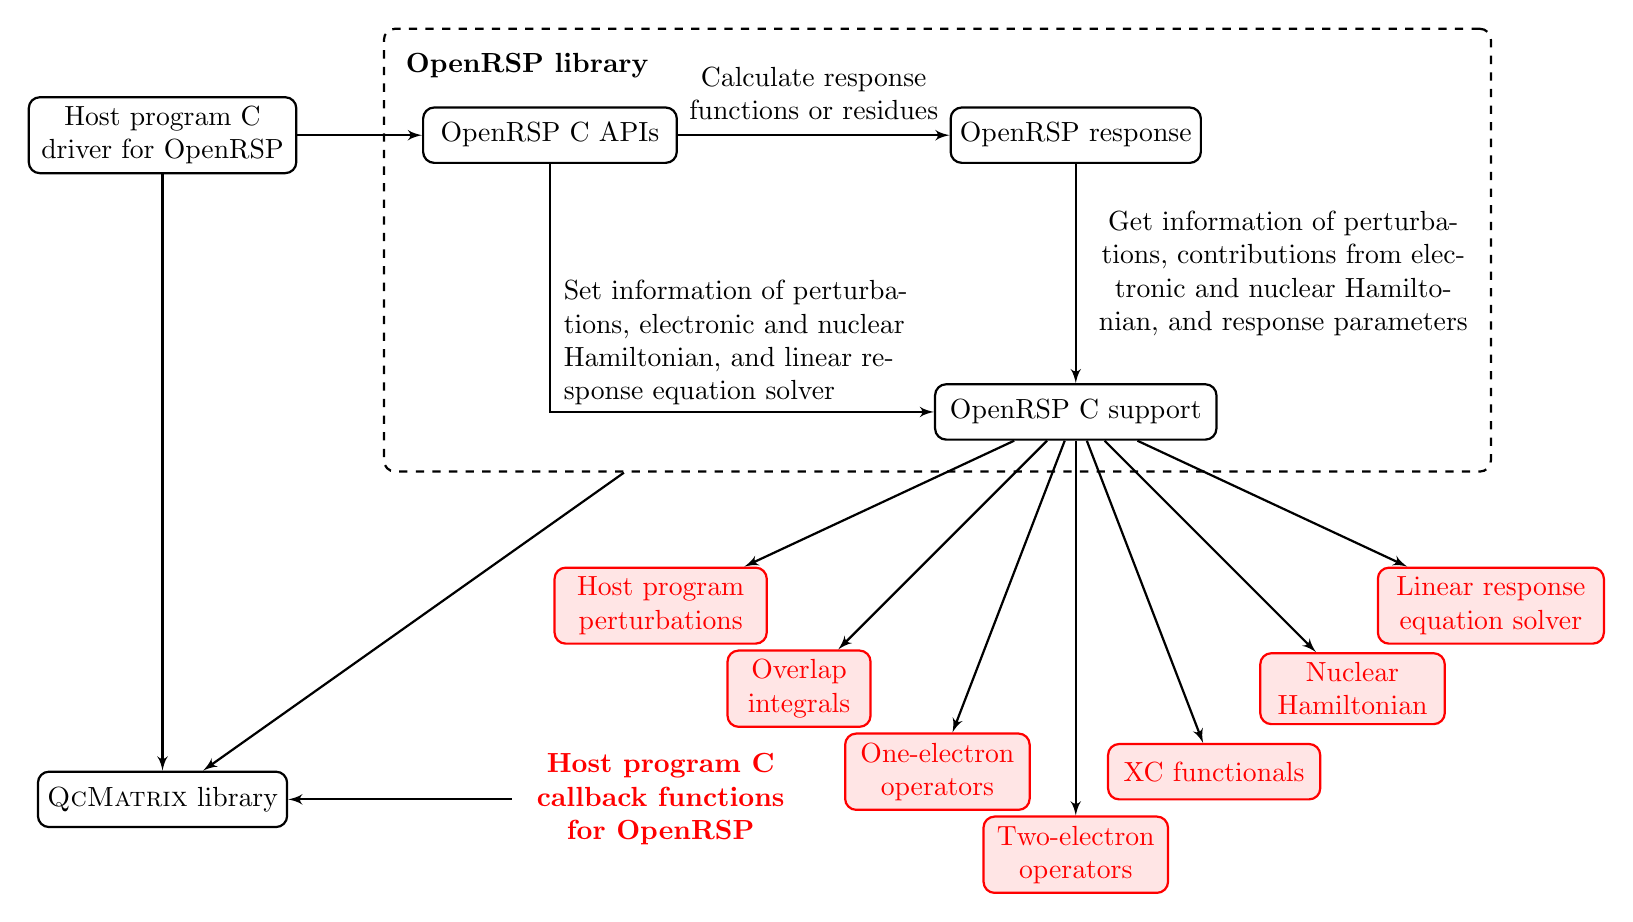
\begin{tikzpicture}[thick]
  \node[color=black, rectangle, draw, text badly centered, rounded corners, %
        minimum height=20] (OpenRSP-response) {OpenRSP response};
  \node[color=black, rectangle, draw, text badly centered, rounded corners, %
        minimum height=20, text width=85, left of=OpenRSP-response, node distance=190] %
       (OpenRSP-C-API) {OpenRSP C APIs};
  \node[color=black, rectangle, draw, text badly centered, rounded corners, %
        minimum height=20, text width=95, below of=OpenRSP-response, node distance=100] %
       (OpenRSP-C-support) {OpenRSP C support};
  \node[color=black, dashed, rectangle, draw, text badly centered, rounded corners, %
        minimum height=160, minimum width=400, above of=OpenRSP-C-API, %
        xshift=140, yshift=-70] (OpenRSP-library) %
       {\begin{minipage}[t][5cm]{13.5cm}\textbf{OpenRSP library}\end{minipage}};
%
  \node[color=black, rectangle, draw, text badly centered, rounded corners, %
        minimum height=20, text width=90, left of=OpenRSP-C-API, node distance=140] %
       (HostDriver) {Host program C driver for OpenRSP};
%
  \node[color=red, fill=red!10, rectangle, draw, text badly centered, rounded corners, %
        minimum height=20, text width=70, below of=OpenRSP-C-support, node distance=70, %
        xshift=-150, yshift=0] (Perturbations) {Host program perturbations};
  \node[color=red, fill=red!10, rectangle, draw, text badly centered, rounded corners, %
        minimum height=20, text width=45, below of=OpenRSP-C-support, node distance=70, %
        xshift=-100, yshift=-30] (Overlap) {Overlap integrals};
  \node[color=red, fill=red!10, rectangle, draw, text badly centered, rounded corners, %
        minimum height=20, text width=60, below of=OpenRSP-C-support, node distance=70, %
        xshift=-50, yshift=-60] (OneOper) {One-electron operators};
  \node[color=red, fill=red!10, rectangle, draw, text badly centered, rounded corners, %
        minimum height=20, text width=60, below of=OpenRSP-C-support, node distance=70, %
        xshift=0, yshift=-90] (TwoOper) {Two-electron operators};
  \node[color=red, fill=red!10, rectangle, draw, text badly centered, rounded corners, %
        minimum height=20, text width=70, below of=OpenRSP-C-support, node distance=70, %
        xshift=50, yshift=-60] (XCFun) {XC functionals};
  \node[color=red, fill=red!10, rectangle, draw, text badly centered, rounded corners, %
        minimum height=20, text width=60, below of=OpenRSP-C-support, node distance=70, %
        xshift=100, yshift=-30] (NucHamiltonian) {Nuclear Hamiltonian};
  \node[color=red, fill=red!10, rectangle, draw, text badly centered, rounded corners, %
        minimum height=20, text width=75, below of=OpenRSP-C-support, node distance=70, %
        xshift=150, yshift=0] (Solver) {Linear response equation solver};
  \node[color=red, text badly centered, minimum height=20, text width=100, %
        below of=HostDriver, node distance=240, xshift=180, yshift=0] (Callback) %
       {\textbf{Host program C callback functions for OpenRSP}};
%
  \node[color=black, rectangle, draw, text badly centered, rounded corners, %
        minimum height=20, below of=HostDriver, node distance=240] %
       (QcMatrix) {\textsc{QcMatrix} library};
%
%  \draw [-latex'] (HostDriver) edge node[align=center, midway, yshift=15, text width=120] %
%    {OpenRSP APIs (C or Fortran)} (OpenRSP);
  \draw [-latex'] (OpenRSP-C-API) edge node[align=center, midway, yshift=15, text width=120] %
    {Calculate response functions or residues} (OpenRSP-response);
  \draw [-latex'] (OpenRSP-response) edge node[align=center, midway, xshift=75, text width=160] %
    {Get information of perturbations, contributions from electronic and nuclear Hamiltonian, %
     and response parameters} (OpenRSP-C-support);
  \draw [-latex'] (OpenRSP-C-API) -- %
    node[at end, align=left, xshift=75, yshift=25, text width=140] %
    {Set information of perturbations, electronic and nuclear Hamiltonian, and linear response %
     equation solver} (OpenRSP-C-API |- OpenRSP-C-support) |- (OpenRSP-C-support);
  \draw [-latex'] (OpenRSP-library)--(QcMatrix);
  \draw [-latex'] (HostDriver)--(OpenRSP-C-API);
  \draw [-latex'] (OpenRSP-C-support)--(Perturbations);
  \draw [-latex'] (OpenRSP-C-support)--(Overlap);
  \draw [-latex'] (OpenRSP-C-support)--(OneOper);
  \draw [-latex'] (OpenRSP-C-support)--(TwoOper);
  \draw [-latex'] (OpenRSP-C-support)--(XCFun);
  \draw [-latex'] (OpenRSP-C-support)--(NucHamiltonian);
  \draw [-latex'] (OpenRSP-C-support)--(Solver);
  \draw [-latex'] (HostDriver)--(QcMatrix);
  \draw [-latex'] (Callback)--(QcMatrix);
\end{tikzpicture}

\end{document}
}
  \caption{OpenRSP used in a C host program.}
  \label{fig-openrsp-framework}
\end{figure}

As shown in Figure~\ref{fig-openrsp-framework}, the OpenRSP library is divided
into three parts:
\begin{enumerate}
  \item The ``OpenRSP C APIs'' work mostly between the host program driver
    routine and other parts of the OpenRSP library, that all the information
    saved in the ``OpenRSP C support'' will be set up by calling the
    corresponding OpenRSP C API;
  \item The ``OpenRSP response'' is the core part in which the performance
    of response theory will be done;
  \item The ``OpenRSP C support'' saves the information of perturbations,
    electronic and nuclear Hamiltonian and linear response equation solver,
    and will be used by the ``OpenRSP response'' part during calculating
    response functions and residues.
\end{enumerate}

The ``OpenRSP response'' was already implemented using Fortran for the AO
based density matrix response theory (source codes in \texttt{src/ao\_dens})
that will not be covered here.

\subsection{Perturbations}
\label{subsection-analysis-perturbation}

For perturbations in OpenRSP, we introduce the following notations and
convention:
\begin{description}
  \item[Perturbation] is described by a label ($a$), a complex frequency
    ($\omega$) and its order ($n$), and written as $a_{\omega}^{n}$ Any
    two perturbations are different if they have different labels, and/or
    frequencies, and/or orders.
  \item[Perturbation label] is an integer distinguishing one perturbation
    from others; all \textit{different} perturbation labels involved in the
    calculations should be given by calling the application programming
    interface (API) \texttt{OpenRSPSetPerturbations()}; OpenRSP will stop if
    there is any unspecified perturbation label given afterwards when calling
    the APIs \texttt{OpenRSPGetRSPFun()} or \texttt{OpenRSPGetResidue()}.
  \item[Perturbation order] Each perturbation can acting on molecules once
    or many times, that is the order of the perturbation.
  \item[Perturbation components and their ranks] Each perturbation may have
    different numbers of components for their different orders, the position
    of each component is called its rank.

    For instance, there will usually be $x,y,z$ components for the electric
    dipole perturbation, and their ranks are \texttt{\{0,1,2\}} in zero-based
    numbering, or \texttt{\{1,2,3\}} in one-based numbering.
  \item[Perturbation tuple] An ordered list of perturbation labels, and in
    which we further require that \textit{identical perturbation labels should
    be consecutive}. That means the tuple $(a,b,b,c)$ is allowed, but $(a,b,c,b)$
    is illegal because the identical labels $b$ are not consecutive.

    As a tuple:
    \begin{enumerate}
      \item Multiple instances of the same labels are allowed so that
        $(a,b,b,c)\ne(a,b,c)$, and
      \item The perturbation labels are ordered so that $(a,b,c)\ne(a,c,b)$
        (because their corresponding response functions or residues are in
        different shapes).
    \end{enumerate}
    We will sometimes use an abbreviated form of perturbation tuple as,
    for instance $abc\equiv(a,b,c)$.

    Obviously, a perturbation tuple $+$ its corresponding complex
    frequencies for each perturbation label can be viewed as a set of
    perturbations, in which the number of times a label (with the same
    frequency) appears is the order of the corresponding perturbation.

    For example, a tuple $(a,b,b,c)$ $+$ its complex frequencies
    $(\omega_{a},\omega_{b},\omega_{b},\omega_{c})$ define perturbations
    $a_{\omega_{a}}^{1}$, $b_{\omega_{b}}^{2}$ and $c_{\omega_{c}}^{1}$;
    another tuple $(a,b,b,c)$ $+$ different complex frequencies for labels
    $b$---$(\omega_{a},\omega_{b_{1}},\omega_{b_{2}},\omega_{c})$ define
    different perturbations $a_{\omega_{a}}^{1}$, $b_{\omega_{b_{1}}}^{1}$,
    $b_{\omega_{b_{2}}}^{1}$ and $c_{\omega_{c}}^{1}$.
  \item[Category of perturbation frequencies] We use different integers for
    distinguishing different values of frequencies within a frequency
    configuration. The category arrary is determined by:
    \begin{enumerate}
      \item For each frequency configuration, we start at the first
        perturbation and let its frequency value be designated number 1, then
      \item For the next perturbation,
        \begin{enumerate}
          \item If its frequency value corresponds to a frequency value
            encountered previously in this frequency, then use the same
            designation as for that previously encountered frequency value, or
          \item If its frequency value has not been encountered before, then
            let that frequency value be designated with the first unused
            number;
        \end{enumerate}
      \item Continue like this until the end of the perturbation tuple;
      \item Start the numbering over again at the next frequency configuration.
    \end{enumerate}
  \item[Canonical order]~
    \begin{enumerate}
      \item In OpenRSP, all perturbation tuples are canonically orderd
        according to the argument \texttt{pert\_tuple} in the
        \texttt{OpenRSPGetRSPFun()} or \texttt{OpenRSPGetResidue()}. For
        instance, when a perturbation tuple $(a,b,c)$ given as
        \texttt{pert\_tuple} in the API \texttt{OpenRSPGetRSPFun()},
        OpenRSP will use such order ($a>b>c$) to arrange all perturbation
        tuples inside and sent to the callback functions.
      \item Moreover, a collection of several perturbation tuples will also
        follow the canonical order. For instance, a collection of all possible
        perturbation tuples of labels $a,b,c,d$ are
        $(0,a,b,ab,c,ac,bc,abc,d,ad,bd,abd,cd,acd,bcd,abcd)$, where $0$ means
        unperturbed quantities that is always the first one in the collection.
    \end{enumerate}
  \item[Perturbation $a$] The first perturbation label in the tuple sent to
    OpenRSP APIs \texttt{OpenRSPGetRSPFun()} or \texttt{OpenRSPGetResidue()},
    are the perturbation $a$~\cite{Thorvaldsen-JCP-129-214108}.
  \item[Perturbation addressing]~
    \begin{enumerate}
      \item The addressing of perturbation labels in a tuple, as mentioned in
        the term \textbf{Canonical order}, is decided by
        \begin{enumerate}
          \item the argument \texttt{pert\_tuple} sent to the API
            \texttt{OpenRSPGetRSPFun()} or \texttt{OpenRSPGetResidue()}, and
          \item the canonical order that OpenRSP uses.
        \end{enumerate}
      \item The addressing of components per perturbation (several consecutive
        identical labels with the same complex frequency) are decided by the
        host program, as will be discussed in the following
        \textbf{perturbation free scheme}.
      \item The addressing of a collection of perturbation tuples follows the
        canonical order as aforementioned.
    \end{enumerate}

    Therefore, the shape of response functions or residues is mostly decided
    by the host program. Take $\mathcal{E}^{abbc}$ for example, its shape is
    $(N_{a},N_{bb},N_{c})$, where $N_{a}$ and $N_{c}$ are respectively the
    numbers of components of the first order of the perturbations $a$ and $c$,
    and $N_{bb}$ is the number of components of the second order of the
    perturbation $b$, and
    \begin{enumerate}
      \item In OpenRSP, we will use notation \texttt{[a][bb][c]} for
        $\mathcal{E}^{abbc}$, where the leftmost index (\texttt{a}) runs
        slowest in memory and the rightmost index (\texttt{c}) runs fastest.
        However, one should be aware that the results are still in a
        one-dimensional array.
      \item If there two different frequencies for the perturbation label
        $b$, OpenRSP will return \texttt{[a][b1][b2][c]}, where \texttt{b1}
        and \texttt{b2} stand for the components of the first order of the
        perturbation $b$.
      \item The notation for a collection of perturbation tuples (still in a
        one-dimensional array) is
        \texttt{\{1,[a],[b],[a][b],[c],[a][c],[b][c],[a][b][c]\}}
        for $(0,a,b,ab,c,ac,bc,abc)$, where as aforementioned the first one
        is the unperturbed quantities.
    \end{enumerate}
\end{description}

\subsubsection{Perturbation Free Scheme}

Now, let us discuss our \textbf{perturbation free scheme}. As aforementioned,
there could be \textbf{different numbers of components} for different
perturbations. In different host programs, these components could \textbf{be
arranged in different ways}.

For instance, there are 9 components for the second order magnetic derivatives
in a redundant way $xx,xy,xz,yx,yy,yz,zx,zy,zz$, but 6 components in a
non-redundant way $xx,xy,xz,yy,yz,zz$. There are at most four centers in
different integrals, non-zero high order ($\ge 5$) geometric derivatives are
only those with at most four differentiated centers.

To take all the above information into account in OpenRSP will make it so
complicated and not necessary, because response theory actually does not care
about the detailed knowledge of different perturbations. In particular, when
all the (perturbed) integrals and expectation values are computed by the host
program's callback functions, the detailed information of perturbations:
\begin{enumerate}
  \item the number of components, and
  \item how they are arranged in memory
\end{enumerate}
can be hidden from OpenRSP.

The former can be easily solved by sending the numbers of components of
different perturbation labels (up to their maximum orders) to the OpenRSP API
\texttt{OpenRSPSetPerturbations()}.

The latter can be important for OpenRSP to construct higher-order derivatives
from lower-order ones. We have two cases:
\begin{enumerate}
  \item Higher-order derivatives are taken with respect to different
    perturbations, for instance, $\frac{\partial^{3}}{\partial a\partial b\partial c}$
    are simply the direct product of components of lower-order derivatives
    with respect to each perturbation $\frac{\partial}{\partial a}$,
    $\frac{\partial}{\partial b}$ and $\frac{\partial}{\partial c}$.
  \item Higher-order derivatives are taken with respect to
    \textbf{one perturbation}. Take the second order-derivatives (in the
    redundant format) for example, they can be constructed from the
    first-order ones as,
    \begin{align*}
      x+x\rightarrow xx,\;\; & 0+0\rightarrow 0,\\
      x+y\rightarrow xy,\;\; & 0+1\rightarrow 1,\\
      x+z\rightarrow xz,\;\; & 0+2\rightarrow 2,\\
      y+x\rightarrow yx,\;\; & 1+0\rightarrow 3,\\
      y+y\rightarrow yy,\;\; & 1+1\rightarrow 4,\\
      y+z\rightarrow yz,\;\; & 1+2\rightarrow 5,\\
      z+x\rightarrow zx,\;\; & 2+0\rightarrow 6,\\
      z+y\rightarrow zy,\;\; & 2+1\rightarrow 7,\\
      z+z\rightarrow zz,\;\; & 2+2\rightarrow 8,
    \end{align*}
    where we have ranked different components in zero-based numbering (numbers
    on the right).

    Because the ranks can be different in different host programs, also the
    above mapping relationship between lower- and higher-order derivatives
    (with respect to \textbf{one perturbation}) can be different in different
    host programs.

    We therefore ask for a callback function \texttt{get\_pert\_concatenation()}
    from host programs. This callback function will, from given components of
    a \textbf{concatenated perturbation tuple} (i.e. higher-order derivatives
    with respect to one perturbation), get the ranks of components of the
    \textbf{sub-perturbation tuples with the same perturbation label} (i.e.
    lower-order derivatives with respect to one perturbation).
\end{enumerate}

As such, the numbers of different components of perturbations and their ranks
are totally decided by the host program---that is the
\textbf{perturbation free scheme}.

%\subsubsection{Internal Perturbation Labels}
%
%As mentioned in our notations and convention, perturbations even with the same
%perturbation label, are different if they have different frequencies. Inside
%OpenRSP, we need to distinguish this kind of different perturbations---same
%perturbation label but different frequencies.
%
%We therefore use internal perturbation labels inside OpenRSP. To avoid
%introduce new \texttt{struct} for perturbation labels, we use unsigned integers
%for both host program's perturbation labels and OpenRSP internal perturbation
%labels.
%
%\begin{figure}[hbt]
%  \centering
%  \scalebox{0.9}{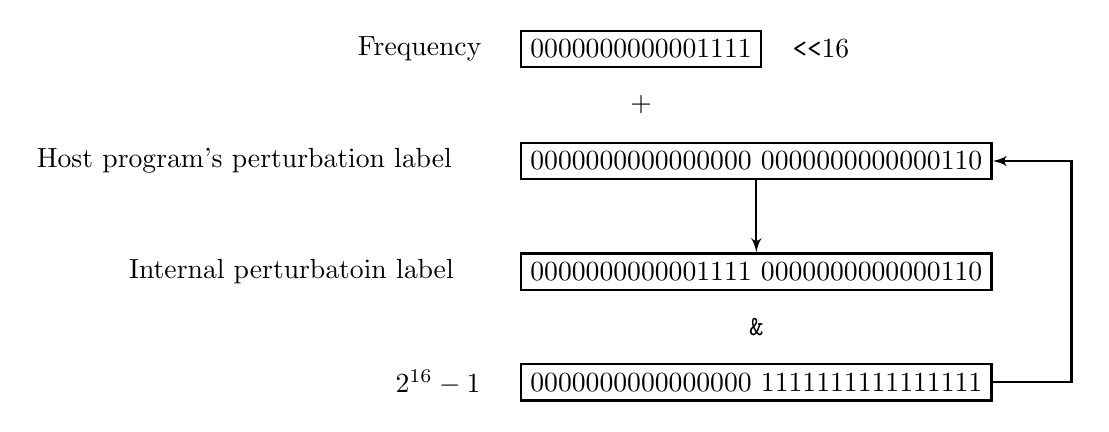
\begin{tikzpicture}[thick]
    \node[rectangle, draw](Frequency) at(0,0) {$0000000000001111$};
    \node[left of=Frequency, node distance=80] {Frequency};
    \node[right of=Frequency, node distance=65] {\texttt{<<}16};
    \node[below of=Frequency, node distance=20] {$+$};
    \node[below=of Frequency.west, anchor=west, yshift=-12, %
      rectangle, draw] (HostLabel) {$0000000000000000$ $0000000000000110$};
    \node[left of=HostLabel, node distance=185] %
      {Host program's perturbation label};
    \node[below of=HostLabel, node distance=40, rectangle, draw] %
      (InternalLabel) {$0000000000001111$ $0000000000000110$};
    \node[left of=InternalLabel, node distance=168] %
      {Internal perturbatoin label};
    \draw[-latex'](HostLabel)--(InternalLabel);
%
    \node[below of=InternalLabel, node distance=20] {\texttt{\&}};
    \node[below of=InternalLabel, node distance=40, rectangle, draw] %
      (Filter) {$0000000000000000$ $1111111111111111$};
    \node[left of=Filter, node distance=115] {$2^{16}-1$};
    \draw[-latex'](Filter.east)--++(1,0)node{~}|-(HostLabel.east);
\end{tikzpicture}
}
%  \caption{Perturbation labels in OpenRSP.}
%  \label{fig-perturbation-label}
%\end{figure}
%
%As illustrated in Figure~\ref{fig-perturbation-label}, if one uses lower $16$
%bits for a host program's label and higher $16$ bits for a frequency in the
%$32$-bit unsigned integers, and if both the host program's label and the
%frequency are marked from $0$ up to $2^{16}-1=65535$, OpenRSP can thus treat
%$2^{16}=65536$ different perturbation labels and different frequencies, which
%is enough for the current response theory calculations. If one uses $64$-bit
%unsigned integers, OpenRSP can then treat more perturbation labels and
%frequencies.

%CCCCCCCCCCCCCCCCCCCCCCCCCCCCCCCCCCCCCCCCCCCCCCCCCCCCCCCCCCCCCCCCCCCCCC

%\subsection{Internal Perturbation Labels}
%\label{subsection-OpenRSP-intern-pert}
%
%As described in Figure~\ref{fig-perturbation-label}, we will use an unsigned
%integer to represent perturbation labels for both the host program and the
%internal use of OpenRSP. The type of this unsigned integer
%[[QcPertInt]]\index{[[QcPertInt]]} is defined as follows:
%<<RSPPertBasicTypes>>=
%/* <macrodef name='OPENRSP_PERT_SHORT_INT'>
%     Represent perturbation labels using unsigned short integers
%   </macrodef> */
%#if defined(OPENRSP_PERT_SHORT_INT)
%/* <datatype name='QcPertInt'>
%     Data type of integers to represent perturbation labels
%   </datatype>
%   <constant name='QCPERTINT_MAX'>
%     Maximal value of an object of the <QcPertInt> type
%   </constant>
%   <constant name='QCPERTINT_FMT'>
%     Format string of <QcPertInt> type
%   </constant> */
%typedef unsigned short QcPertInt;
%#define QCPERTINT_MAX USHRT_MAX
%#define QCPERTINT_FMT "hu"
%/* <macrodef name='OPENRSP_PERT_INT'>
%     Represent perturbation labels using unsigned integers
%   </macrodef> */
%#elif defined(OPENRSP_PERT_INT)
%typedef unsigned int QcPertInt;
%#define QCPERTINT_MAX UINT_MAX
%#define QCPERTINT_FMT "u"
%#else
%typedef unsigned long QcPertInt;
%#define QCPERTINT_MAX ULONG_MAX
%#define QCPERTINT_FMT "lu"
%#endif
%@ Here we allow users to choose either
%[[unsigned short]]\index{[[OPENRSP_PERT_SHORT_INT]]},
%[[unsigned int]]\index{[[OPENRSP_PERT_INT]]}, or [[unsigned long]] for the
%type [[QcPertInt]]. We also define a constant
%[[QCPERTINT_MAX]]\index{[[QCPERTINT_MAX]]} for the maximal value of an object
%of the [[QcPertInt]] type, and a format string
%([[QCPERTINT_FMT]]\index{[[QCPERTINT_FMT]]}) of the [[QcPertInt]] type.
%
%We futher allow users to set the number of bits in an object of [[QcPertInt]]
%for representing the host program's perturbation labels (see
%Figure~\ref{fig-perturbation-label}). This can be done by changing the constant
%[[OPENRSP_PERT_LABEL_BIT]]\index{[[OPENRSP_PERT_LABEL_BIT]]} during building:
%<<RSPPertBasicTypes>>=
%/* <macrodef name='OPENRSP_PERT_LABEL_BIT'>
%     Set <OPENRSP_PERT_LABEL_BIT>
%   </macrodef>
%   <constant name='OPENRSP_PERT_LABEL_BIT'>
%     Number of bits in an object of <QcPertInt> type for a perturbation label
%   </constant> */
%#if !defined(OPENRSP_PERT_LABEL_BIT)
%#define OPENRSP_PERT_LABEL_BIT 10
%#endif
%@ and from which, and from the knowledge of [[QCPERTINT_MAX]] we can compute
%[[OPENRSP_PERT_LABEL_MAX]]\index{[[OPENRSP_PERT_LABEL_MAX]]} and
%[[OPENRSP_NUM_FREQ_MAX]]\index{[[OPENRSP_NUM_FREQ_MAX]]}, which are the maximal
%values of perturbation labels and the number of frequencies allowed:
%<<RSPPertBasicTypes>>=
%/* <constant name='OPENRSP_PERT_LABEL_MAX'>
%     Maximal value for perturbation labels
%   </constant>
%   <constant name='OPENRSP_NUM_FREQ_MAX'>
%     Maximal value for number of frequencies
%   </constant> */
%extern const QcPertInt OPENRSP_PERT_LABEL_MAX;
%extern const QcPertInt OPENRSP_NUM_FREQ_MAX;
%@ Here, to avoid multiple inclusions of the header file that will lead to
%multiple definitions, we have the following implementation file for the
%[[OPENRSP_PERT_LABEL_MAX]] and [[OPENRSP_NUM_FREQ_MAX]]:
%<<RSPPertLabel.c>>=
%/*
%  <<OpenRSPLicense>>
%*/
%
%#include "RSPPerturbation.h"
%
%/* see https://scaryreasoner.wordpress.com/2009/02/28/checking-sizeof-at-compile-time
%   accessing date Oct. 6, 2015 */
%#define QC_BUILD_BUG_ON(condition) ((void)sizeof(char[1 - 2*!!(condition)]))
%void RSPPertCheckLabelBit()
%{
%    QC_BUILD_BUG_ON(sizeof(QCPERTINT_MAX)*CHAR_BIT<=OPENRSP_PERT_LABEL_BIT);
%}
%
%const QcPertInt OPENRSP_PERT_LABEL_MAX = (1<<OPENRSP_PERT_LABEL_BIT)-1;
%const QcPertInt OPENRSP_NUM_FREQ_MAX =
%                (QCPERTINT_MAX-OPENRSP_PERT_LABEL_MAX)>>OPENRSP_PERT_LABEL_BIT;
%@ The function [[RSPPertCheckLabelBit()]] ensures that
%[[OPENRSP_PERT_LABEL_BIT]] is not too large and there are still bits left for
%the number of frequencies. One will have building error when compiling the
%function [[RSPPertCheckLabelBit()]] if [[OPENRSP_PERT_LABEL_BIT]] is too large.
%
%However, the function [[RSPPertCheckLabelBit()]] can not guarantee the above
%setting ([[QcPertInt]] type and [[OPENRSP_PERT_LABEL_BIT]]) is enough for
%holding the host program's perturbation labels and the number of frequencies.
%This will be checked against [[OPENRSP_PERT_LABEL_MAX]] and
%[[OPENRSP_NUM_FREQ_MAX]] by OpenRSP when (i) setting the host program's
%perturbations, and (ii) calculating response functions or residues.

%\subsection{Conversion of Perturbation Tuples and Labels}
%\label{subsection-OpenRSP-convert-pert}
%
%As described in Figure~\ref{fig-perturbation-label}, we need to convert the
%host program's perturbation labels and frequencies into OpenRSP internal
%perturbation labels when calculating response functions or residues:
%<<RSPertAPIs>>=
%extern QErrorCode RSPPertTupleHostToInternal(const RSPPert*,
%                                             const QInt,
%                                             const QInt*,
%                                             const QInt,
%                                             const QReal*,
%                                             QInt*,
%                                             QReal*);
%@ This function first looks through a given host program's perturbation tuple
%to find consecutive identical pertubation labels, and then checks how many
%different frequencies associated with the consecutive identical labels:
%<<RSPPerturbation.c>>=
%/* <function name='RSPPertTupleHostToInternal'
%             attr='private'
%             author='Bin Gao'
%             date='2015-10-08'>
%     Convert a host program's perturbation tuple to an internal pertubation tuple
%     <param name='rsp_pert' direction='in'>
%       The context of perturbations
%     </param>
%     <param name='len_tuple' direction='in'>
%       Length of the host program's and the internal perturbation tuples
%     </param>
%     <param name='pert_tuple' direction='in'>
%       The host program's perturbation tuple, in which identical perturbation
%       labels should be consecutive, and the first one is the perturbation $a$
%     </param>
%     <param name='num_freq_configs' direction='in'>
%       Number of different frequency configurations
%     </param>
%     <param name='pert_freqs' direction='in'>
%       Complex frequencies of each perturbation label (except for the
%       perturbation $a$) over all frequency configurations, size is therefore
%       $2\times[(<len_tuple>-1)\times<num_freq_configs>]$, and arranged as
%       <c>[num_freq_configs][len_tuple-1][2]</c> in memory (that is, the real
%       and imaginary parts of each frequency are consecutive in memory)
%     </param>
%     <param name='intern_pert_tuple' direction='out'>
%       The internal perturbation tuple, in which identical perturbation
%       labels are consecutive, and the first one is the perturbation $a$
%     </param>
%     <param name='intern_pert_freqs' direction='out'>
%       Complex frequencies of each perturbation label (including the
%       perturbation $a$) over all frequency configurations, size is therefore
%       $2\times<len_tuple>\times<num_freq_configs>$, and arranged as
%       <c>[num_freq_configs][len_tuple][2]</c> in memory (that is, the real and
%       imaginary parts of each frequency are consecutive in memory)
%     </param>
%     <return>Error information</return>
%   </function> */
%QErrorCode RSPPertTupleHostToInternal(const RSPPert *rsp_pert,
%                                      const QInt len_tuple,
%                                      const QInt *pert_tuple,
%                                      const QInt num_freq_configs,
%                                      const QReal *pert_freqs,
%                                      QInt *intern_pert_tuple,
%                                      QReal *intern_pert_freqs)
%{
%    QInt ipert,jpert;  /* incremental recorders */
%    QInt first_id;     /* first identical pertubation label in the tuple */
%    QInt last_id;      /* last identical pertubation label in the tuple */
%    QBool non_id;      /* indicates if non-identical label found */
%
%    /* we first try to find consecutive identical pertubation labels */
%    first_id = 0;
%    non_id = QFALSE;
%    for (ipert=first_id; ipert<len_tuple-1; ipert++) {
%        if (pert_tuple[ipert]!=pert_tuple[ipert+1]) {
%            last_id = ipert;
%            non_id = QTRUE;
%            break;
%        }
%    }
%    if (non_id=QTRUE) {
%    }
%    else {
%    }
%    /* loops over all known perturbation labels and checks if they are in the tuple */
%    for (ipert=0; ipert<rsp_pert->num_pert; ipert++) {
%        /* loops over perturbation labels in the tuple */
%        for (ipert=first_id; ipert<len_tuple; ipert++) {
%            /* checks if the given label is known */
%            if (pert_tuple[ipert]==rsp_pert->pert_labels[jpert]) {
%                
%            }
%        }
%    }
%    return QSUCCESS;
%}
%
%@ where we have also checked the numbers of different frequencies against
%[[OPENRSP_NUM_FREQ_MAX]].
%
%After converting into internal perturbation labels, OpenRSP will usually use
%its internal perturbation tuples (described by the internal perturbation
%labels) and the corresponding complex frequencies in calculations.
%
%However, when making a callback, (i) the complex frequencies will not be
%passed, and (ii) internal perturbation labels will be converted into host
%program's ones. The callback functions can therefore not distinguish different
%perturbations only from the host program's perturbation labels.
%
%For instance, a host program's perturbation tuple $(a,b,b,c)$ and the
%corresponding complex frequencies
%$(\omega_{a},\omega_{b_{1}},\omega_{b_{2}},\omega_{c})$ actually define four
%different perturbations $a_{\omega_{a}}^{1}$, $b_{\omega_{b_{1}}}^{1}$,
%$b_{\omega_{b_{2}}}^{1}$ and $c_{\omega_{c}}^{1}$ instead of three (each
%perturbation label $b$ defines one perturbation).
%
%We therefore need to pass both the host program's perturbation labels
%$(a,b,b,c)$ and their associated orders $(1,1,1,1)$ to callback functions,
%together meaning the passed two perturbation labels $b$ stand for two different
%perturbations, and both of them are the first-order perturbation.
%
%The following function will convert an internal perturbation tuple to the host
%program's pertubation labels and their orders:
%<<RSPertAPIs>>=
%extern QErrorCode RSPPertInternTupleToHostLabelOrder(const QInt,
%                                                     const QInt*,
%                                                     QInt*,
%                                                     QInt*,
%                                                     QInt*);
%@ and here we assume that \textbf{consecutive identical internal perturbation
%labels is for one perturbation}:
%<<RSPPerturbation.c>>=
%/* <function name='RSPPertInternTupleToHostLabelOrder'
%             attr='private'
%             author='Bin Gao'
%             date='2015-10-08'>
%     Convert an internal perturbation tuple to the host program's pertubation
%     labels and their orders
%     <param name='len_tuple' direction='in'>
%       Length of the internal perturbation tuple
%     </param>
%     <param name='intern_pert_tuple' direction='in'>
%       The internal perturbation tuple
%     </param>
%     <param name='num_pert' direction='out'>
%       Number of different perturbations from the internal perturbation tuple
%     </param>
%     <param name='pert_labels' direction='out'>
%       Host program's pertubation labels of the resulted perturbations
%     </param>
%     <param name='pert_orders' direction='out'>
%       Orders of the resulted perturbations
%     </param>
%     <return>Error information</return>
%   </function> */
%QErrorCode RSPPertInternTupleToHostLabelOrder(const QInt len_tuple,
%                                              const QInt *intern_pert_tuple,
%                                              QInt *num_pert,
%                                              QInt *pert_labels,
%                                              QInt *pert_orders)
%      
%{
%    QInt ilab;   /* incremental recorder over perturbation labels */
%    QInt ipert;  /* incremental recorder for different perturbations */
%    for (ilab=0,ipert=0; ilab<len_tuple; ) {
%        pert_labels[ipert] = intern_pert_tuple[ilab];
%        pert_orders[ipert] = 1;
%        /* finds consecutive identical internal perturbation labels */
%        ilab++;
%        for (; ilab<len_tuple; ) {
%            if (pert_labels[ipert]==intern_pert_tuple[ilab]) {
%                pert_orders[ipert]++;
%            }
%            else {
%                break;
%            }
%            ilab++;
%        }
%        /* converts to the host program's label */
%        pert_labels[ipert] &= OPENRSP_PERT_LABEL_MAX;
%        ipert++;
%    }
%    *num_pert = ipert;
%    return QSUCCESS;
%}
%
%@ where the conversion of the internal label to the host program's label is
%achieved by the bitwise AND operation ([[&=]]) with [[OPENRSP_PERT_LABEL_MAX]]
%as illustrated in Figure~\ref{fig-perturbation-label}.

% XC functional callbacks
%
% [0,a,b,c,d,ab,ac,ad,bc,bd,cd]
% ->
% [0,a,b,d,ab,ad,bc,bd]
% if b==c



% Design
%\input{Design}

% Implementation
%
% weaves all *.nw files together so that one can cross-reference chunks
% in different *.nw files
\nwfilename{/Users/bga006/Work/XKjem/gitlab/openrsp/web/Implementation.nw}\nwbegindocs{0}\chapter{Implementation}
\label{chapter-implementation}

\section{Header File for Users\index{{\tt{}OpenRSP.h}}}

To use \LibName, C users need to include the following header file into
their codes:
\nwenddocs{}\nwbegincode{1}\sublabel{NWImpz-Ope9-1}\nwmargintag{{\nwtagstyle{}\subpageref{NWImpz-Ope9-1}}}\moddef{OpenRSP.h~{\nwtagstyle{}\subpageref{NWImpz-Ope9-1}}}\endmoddef
/*
  \LA{}OpenRSPLicense~{\nwtagstyle{}\subpageref{NWImpz-OpeE-1}}\RA{}

  <header name='OpenRSP.h' author='Bin Gao' date='2014-01-27'>
    The header file of OpenRSP library for users
  </header>
*/

#if !defined(OPENRSP_H)
#define OPENRSP_H

/* host program perturbations */
#include "RSPPerturbation.h"
/* type of electronic wave function */
/*#include "RSPWaveFunction.h"*/
/* overlap integrals */
#include "RSPOverlap.h"
/* one-electron operators */
#include "RSPOneOper.h"
/* two-electron operators */
#include "RSPTwoOper.h"
/* exchange-correlation (XC) functionals */
#include "RSPXCFun.h"
/* nuclear Hamiltonian */
#include "RSPNucHamilton.h"
/* linear response equation solver */
#include "RSPSolver.h"

\LA{}OpenRSPContext~{\nwtagstyle{}\subpageref{NWImpz-OpeE.2-1}}\RA{}

\LA{}OpenRSPAPIs~{\nwtagstyle{}\subpageref{NWImpz-OpeB-1}}\RA{}

#endif

\nwnotused{OpenRSP.h}\nwendcode{}\nwbegindocs{2}Here, the directives {\tt{}{\char35}if\ !defined(OPENRSP{\char95}H)} and {\tt{}{\char35}define\ OPENRSP{\char95}H}
(\textbf{include guard}\index{Include guard}) together prevent the header file
from being compiled more than once.

We plan to release \LibName under the GNU Lesser General Public
License\index{\LibName License}:
\nwenddocs{}\nwbegincode{3}\sublabel{NWImpz-OpeE-1}\nwmargintag{{\nwtagstyle{}\subpageref{NWImpz-OpeE-1}}}\moddef{OpenRSPLicense~{\nwtagstyle{}\subpageref{NWImpz-OpeE-1}}}\endmoddef
OpenRSP: open-ended library for response theory
Copyright 2015 Radovan Bast,
               Daniel H. Friese,
               Bin Gao,
               Dan J. Jonsson,
               Magnus Ringholm,
               Kenneth Ruud,
               Andreas Thorvaldsen

OpenRSP is free software: you can redistribute it and/or modify
it under the terms of the GNU Lesser General Public License as
published by the Free Software Foundation, either version 3 of
the License, or (at your option) any later version.

OpenRSP is distributed in the hope that it will be useful,
but WITHOUT ANY WARRANTY; without even the implied warranty of
MERCHANTABILITY or FITNESS FOR A PARTICULAR PURPOSE. See the
GNU Lesser General Public License for more details.

You should have received a copy of the GNU Lesser General Public
License along with OpenRSP. If not, see <http://www.gnu.org/licenses/>.

\nwused{\\{NWImpz-Ope9-1}\\{NWImpz-OpeF-1}\\{NWImpz-OpeH-1}\\{NWImpz-OpeE.3-1}\\{NWImpz-OpeG-1}\\{NWRSP10-OpeP-1}\\{NWRSP10-RSPH-1}\\{NWRSP10-RSPF-1}\\{NWRSP10-RSPH.2-1}\\{NWRSP10-RSPE-1}\\{NWRSP10-RSPL-1}\\{NWRSP10-RSPP-1}\\{NWRSP10-RSPG-1}\\{NWRSPv-OpeJ-1}\\{NWRSPv-RSPC-1}\\{NWRSPv-RSPI-1}\\{NWRSPv-RSPK-1}\\{NWRSPv-RSPH.4-1}\\{NWRSPv-RSPI.2-1}\\{NWRSPv-RSPI.3-1}\\{NWRSPv-RSPJ.2-1}\\{NWRSPv.2-OpeJ.2-1}\\{NWRSPv.2-RSPC.2-1}\\{NWRSPv.2-RSPI.4-1}\\{NWRSPv.2-RSPF.2-1}\\{NWRSPv.2-RSPK.2-1}\\{NWRSPv.2-RSPH.5-1}\\{NWRSPv.2-RSPI.5-1}\\{NWRSPv.2-RSPI.6-1}\\{NWRSPv.2-RSPJ.3-1}\\{NWRSPv.3-OpeJ.3-1}\\{NWRSPv.3-RSPC.3-1}\\{NWRSPv.3-RSPI.7-1}\\{NWRSPv.3-RSPF.3-1}\\{NWRSPv.3-RSPK.3-1}\\{NWRSPv.3-RSPH.6-1}\\{NWRSPv.3-RSPI.8-1}\\{NWRSPv.3-RSPI.9-1}\\{NWRSPv.3-RSPJ.4-1}\\{NWRSPt-OpeH.2-1}\\{NWRSPt-RSPA-1}\\{NWRSPt-RSPG.2-1}\\{NWRSPt-RSPD-1}\\{NWRSPt-RSPI.A-1}\\{NWRSPt-RSPF.4-1}\\{NWRSPt-RSPG.3-1}\\{NWRSPt-RSPG.4-1}\\{NWRSPt-RSPH.7-1}\\{NWRSPz-OpeN-1}\\{NWRSPz-RSPG.5-1}\\{NWRSPz-RSPM-1}\\{NWRSPz-RSPO-1}\\{NWRSPz-RSPL.2-1}\\{NWRSPz-RSPW-1}\\{NWRSPz-RSPR-1}\\{NWRSPz-RSPN-1}\\{NWRSPu-OpeR-1}\\{NWRSPu-RSPB-1}\\{NWRSPu-RSPH.8-1}\\{NWRSPu-RSPJ.5-1}\\{NWRSPu-RSPG.6-1}\\{NWRSPu-RSPV-1}\\{NWRSPu-RSPI.B-1}\\{NWRes12-OpeI-1}\\{NWRest-OpeJ.4-1}\\{NWForw-OpeN.2-1}}\nwendcode{}\nwbegindocs{4}In the following sections, we will describe how to implement each component
of the ``\LibName C support'' (red blocks in Figure~\ref{fig-openrsp-framework}
under the ``\LibName C support'') and the corresponding ``\LibName C API''.
Each component will have its header file, implemented C {\tt{}struct} and
corresponding functions that can be called inside \LibName.

The \LibName context {\tt{}OpenRSPContext} will encapsulate all the implemented C
{\tt{}struct}'s of the ``\LibName C support'' components into another C
{\tt{}struct}:
\nwenddocs{}\nwbegincode{5}\sublabel{NWImpz-OpeE.2-1}\nwmargintag{{\nwtagstyle{}\subpageref{NWImpz-OpeE.2-1}}}\moddef{OpenRSPContext~{\nwtagstyle{}\subpageref{NWImpz-OpeE.2-1}}}\endmoddef
typedef struct \{
    QBool assembled;               /* indicates if the OpenRSP context assembled */
    RSPPert *rsp_pert;             /* host program perturbations */
    /*ElecWav *elec_wav;*/           /* implementation-specific data of (electronic) wave function */
    /*ElecWavType elec_wav_type;*/
    RSPOverlap *overlap;           /* overlap integrals */
    RSPOneOper *one_oper;          /* one-electron operators */
    RSPTwoOper *two_oper;          /* two-electron operators */
    RSPXCFun *xc_fun;              /* XC functionals */
    RSPNucHamilton *nuc_hamilton;  /* nuclear Hamiltonian */
    RSPSolver *rsp_solver;         /* linear response equation solver */
\} OpenRSP;
\nwused{\\{NWImpz-Ope9-1}}\nwendcode{}\nwbegindocs{6}where we have used types, macros and APIs implemented in the
\textsc{QcMatrix} library and one should be familiar with them first.

Users should use the \LibName context and the following APIs to access the
functionalities of \LibName:
\nwenddocs{}\nwbegincode{7}\sublabel{NWImpz-OpeB-1}\nwmargintag{{\nwtagstyle{}\subpageref{NWImpz-OpeB-1}}}\moddef{OpenRSPAPIs~{\nwtagstyle{}\subpageref{NWImpz-OpeB-1}}}\endmoddef
extern QErrorCode OpenRSPCreate(OpenRSP*);
extern QErrorCode OpenRSPSetPerturbations(OpenRSP*,
                                          const QInt,
                                          const QInt*,
                                          const QInt*,
                                          const QInt*,
#if defined(OPENRSP_C_USER_CONTEXT)
                                          QVoid*,
#endif
                                          const GetPertCat);
/*extern QErrorCode OpenRSPSetWaveFunction(OpenRSP*,const ElecWavType);*/
extern QErrorCode OpenRSPSetOverlap(OpenRSP*,
                                    const QInt,
                                    const QInt*,
                                    const QInt*,
#if defined(OPENRSP_C_USER_CONTEXT)
                                    QVoid*,
#endif
                                    const GetOverlapMat,
                                    const GetOverlapExp);
extern QErrorCode OpenRSPAddOneOper(OpenRSP*,
                                    const QInt,
                                    const QInt*,
                                    const QInt*,
#if defined(OPENRSP_C_USER_CONTEXT)
                                    QVoid*,
#endif
                                    const GetOneOperMat,
                                    const GetOneOperExp);
extern QErrorCode OpenRSPAddTwoOper(OpenRSP*,
                                    const QInt,
                                    const QInt*,
                                    const QInt*,
#if defined(OPENRSP_C_USER_CONTEXT)
                                    QVoid*,
#endif
                                    const GetTwoOperMat,
                                    const GetTwoOperExp);
extern QErrorCode OpenRSPAddXCFun(OpenRSP*,
                                  const QInt,
                                  const QInt*,
                                  const QInt*,
#if defined(OPENRSP_C_USER_CONTEXT)
                                  QVoid*,
#endif
                                  const GetXCFunMat,
                                  const GetXCFunExp);
extern QErrorCode OpenRSPSetNucHamilton(OpenRSP*,
                                        const QInt,
                                        const QInt*,
                                        const QInt*,
#if defined(OPENRSP_C_USER_CONTEXT)
                                        QVoid*,
#endif 
                                        const GetNucContrib,
/*FIXME: num_atoms to be removed after perturbation free scheme implemented*/
                                        const QInt);
extern QErrorCode OpenRSPSetLinearRSPSolver(OpenRSP*,
#if defined(OPENRSP_C_USER_CONTEXT)
                                            QVoid*,
#endif
                                            const GetLinearRSPSolution);
extern QErrorCode OpenRSPAssemble(OpenRSP*);
extern QErrorCode OpenRSPWrite(const OpenRSP*,const QChar*);
extern QErrorCode OpenRSPGetRSPFun(OpenRSP*,
                                   const QcMat*,
                                   const QcMat*,
                                   const QcMat*,
                                   const QInt,
                                   const QInt*,
                                   const QInt*,
                                   const QInt*,
                                   const QReal*,
                                   const QInt*,
                                   const QInt,
                                   QReal*);
extern QErrorCode OpenRSPGetResidue(OpenRSP*,
                                    const QcMat*,
                                    const QcMat*,
                                    const QcMat*,
                                    const QInt,
                                    const QInt,
                                    const QReal*,
                                    QcMat*[],
                                    const QInt,
                                    const QInt*,
                                    const QInt*,
                                    const QInt*,
                                    const QInt*,
                                    const QInt*,
                                    const QReal*,
                                    const QInt*,
                                    const QInt,
                                    QReal*);
extern QErrorCode OpenRSPDestroy(OpenRSP*);

\nwused{\\{NWImpz-Ope9-1}}\nwendcode{}\nwbegindocs{8}Here, we have also introduced the type of electronic wave function, but which
has not been implemented.

Last but not least, the directive
\begin{Verbatim}
#if defined(OPENRSP_C_USER_CONTEXT)
                                            QVoid*,
#endif
\end{Verbatim}
in most \LibName APIs enables users to provide their necessary setting for the
callback functions that \LibName will send it back when invoking the callback
functions. For instance, users can provide the information of basis sets to
\LibName and use it inside the callback functions for different integral
calculations.

\section{Four Basic APIs for the \LibName Context}

In this section, we will implement four basic APIs {\tt{}OpenRSPCreate()},
{\tt{}OpenRSPAssemble()}, {\tt{}OpenRSPWrite()} and {\tt{}OpenRSPDestroy()}, while other
APIs will be implemented in the following sections. These four APIs
respectively create, assemble, write and destroy the \LibName context.

The API {\tt{}OpenRSPCreate()} is very simple as it only initializes the pointers
of the context:
\nwenddocs{}\nwbegincode{9}\sublabel{NWImpz-OpeF-1}\nwmargintag{{\nwtagstyle{}\subpageref{NWImpz-OpeF-1}}}\moddef{OpenRSPCreate.c~{\nwtagstyle{}\subpageref{NWImpz-OpeF-1}}}\endmoddef
/*
  \LA{}OpenRSPLicense~{\nwtagstyle{}\subpageref{NWImpz-OpeE-1}}\RA{}
*/

#include "OpenRSP.h"

/* <function name='OpenRSPCreate' author='Bin Gao' date='2014-01-28'>
     Creates the OpenRSP context
     <param name='open_rsp' direction='inout'>The OpenRSP context</param>
     <return>Error information</return>
   </function> */
QErrorCode OpenRSPCreate(OpenRSP *open_rsp)
\{
    open_rsp->assembled = QFALSE;
    open_rsp->rsp_pert = NULL;
    /*open_rsp->elec_wav = NULL;*/
    /*open_rsp->elec_wav_type = ELEC_AO_D_MATRIX;*/
    open_rsp->overlap = NULL;
    open_rsp->one_oper = NULL;
    open_rsp->two_oper = NULL;
    open_rsp->xc_fun = NULL;
    open_rsp->nuc_hamilton = NULL;
    open_rsp->rsp_solver = NULL;
    return QSUCCESS;
\}

\nwnotused{OpenRSPCreate.c}\nwendcode{}\nwbegindocs{10}The other three APIs are also easy to implement, as they only invoke
functions of the ``\LibName C support'' part to respectively assemble, write
and destroy the corresponding C {\tt{}struct}'s:
\nwenddocs{}\nwbegincode{11}\sublabel{NWImpz-OpeH-1}\nwmargintag{{\nwtagstyle{}\subpageref{NWImpz-OpeH-1}}}\moddef{OpenRSPAssemble.c~{\nwtagstyle{}\subpageref{NWImpz-OpeH-1}}}\endmoddef
/*
  \LA{}OpenRSPLicense~{\nwtagstyle{}\subpageref{NWImpz-OpeE-1}}\RA{}
*/

#include "OpenRSP.h"

/* <function name='OpenRSPAssemble' author='Bin Gao' date='2014-07-30'>
     Assembles the OpenRSP context
     <param name='open_rsp' direction='inout'>The OpenRSP context</param>
     <return>Error information</return>
   </function> */
QErrorCode OpenRSPAssemble(OpenRSP *open_rsp)
\{
    QErrorCode ierr;
    open_rsp->assembled = QFALSE;
    /* assembles host program perturbations */
    if (open_rsp->rsp_pert!=NULL) \{
        ierr = RSPPertAssemble(open_rsp->rsp_pert);
        QErrorCheckCode(ierr, FILE_AND_LINE, "calling RSPPertAssemble()");
    \}
#if defined(OPENRSP_PERTURBATION_FREE)
    else \{
        QErrorExit(FILE_AND_LINE, "perturbations should be set by OpenRSPSetPerturbations()");
    \}
#endif
/*FIXME: to implement ierr = xxAssemble(open_rsp->elec_eom); */
    /* assembles overlap integrals */
    if (open_rsp->overlap!=NULL) \{
        ierr = RSPOverlapAssemble(open_rsp->overlap);
        QErrorCheckCode(ierr, FILE_AND_LINE, "calling RSPOverlapAssemble()");
    \}
    /* assembles one-electron operators */
    if (open_rsp->one_oper!=NULL) \{
        ierr = RSPOneOperAssemble(open_rsp->one_oper);
        QErrorCheckCode(ierr, FILE_AND_LINE, "calling RSPOneOperAssemble()");
    \}
    /* assembles two-electron operators */
    if (open_rsp->two_oper!=NULL) \{
        ierr = RSPTwoOperAssemble(open_rsp->two_oper);
        QErrorCheckCode(ierr, FILE_AND_LINE, "calling RSPTwoOperAssemble()");
    \}
    /* assembles XC functionals */
    if (open_rsp->xc_fun!=NULL) \{
        ierr = RSPXCFunAssemble(open_rsp->xc_fun);
        QErrorCheckCode(ierr, FILE_AND_LINE, "calling RSPXCFunAssemble()");
    \}
    /* assembles nuclear Hamiltonian */
    if (open_rsp->nuc_hamilton!=NULL) \{
        ierr = RSPNucHamiltonAssemble(open_rsp->nuc_hamilton);
        QErrorCheckCode(ierr, FILE_AND_LINE, "calling RSPNucHamiltonAssemble()");
    \}
    /* assembles linear response equation solver */
    if (open_rsp->rsp_solver!=NULL) \{
        ierr = RSPSolverAssemble(open_rsp->rsp_solver);
        QErrorCheckCode(ierr, FILE_AND_LINE, "calling RSPSolverAssemble()");
    \}
    else \{
        QErrorExit(FILE_AND_LINE, "linear response equation solver should be set by OpenRSPSetSolver()");
    \}
    open_rsp->assembled = QTRUE;
    return QSUCCESS;
\}
\nwnotused{OpenRSPAssemble.c}\nwendcode{}\nwbegindocs{12}Here, we will remove the directive {\tt{}{\char35}if\ defined(OPENRSP{\char95}PERTURBATION{\char95}FREE)}
after the \textbf{perturbation free scheme} implemented.

\nwenddocs{}\nwbegincode{13}\sublabel{NWImpz-OpeE.3-1}\nwmargintag{{\nwtagstyle{}\subpageref{NWImpz-OpeE.3-1}}}\moddef{OpenRSPWrite.c~{\nwtagstyle{}\subpageref{NWImpz-OpeE.3-1}}}\endmoddef
/*
  \LA{}OpenRSPLicense~{\nwtagstyle{}\subpageref{NWImpz-OpeE-1}}\RA{}
*/

#include "OpenRSP.h"

/* <function name='OpenRSPWrite' author='Bin Gao' date='2014-07-30'>
     Writes the OpenRSP context
     <param name='open_rsp' direction='in'>The OpenRSP context</param>
     <param name='file_name' direction='in'>File to write the context</param>
     <return>Error information</return>
   </function> */
QErrorCode OpenRSPWrite(const OpenRSP *open_rsp, const QChar *file_name)
\{
    FILE *fp_rsp;     /* file pointer */
    QErrorCode ierr;  /* error information */
    /* opens the file */
    fp_rsp = fopen(file_name, "a");
    if (fp_rsp==NULL) \{
        printf("OpenRSPWrite>> file: %s\\n", file_name);
        QErrorExit(FILE_AND_LINE, "failed to open the file in appending mode");
    \}
    fprintf(fp_rsp, "\\nOpenRSP library compiled at %s, %s\\n", __TIME__, __DATE__);
    /* context of the (electronic) wave function */
    /*FIXME: ierr = xxWrite(open_rsp->elec_eom); */
    if (open_rsp->rsp_pert!=NULL) \{
        ierr = RSPPertWrite(open_rsp->rsp_pert, fp_rsp);
        QErrorCheckCode(ierr, FILE_AND_LINE, "calling RSPPertWrite()");
    \}
    if (open_rsp->overlap!=NULL) \{
        fprintf(fp_rsp, "OpenRSPWrite>> overlap integrals\\n");
        ierr = RSPOverlapWrite(open_rsp->overlap, fp_rsp);
        QErrorCheckCode(ierr, FILE_AND_LINE, "calling RSPOverlapWrite()");
    \}
    if (open_rsp->one_oper!=NULL) \{
        fprintf(fp_rsp, "OpenRSPWrite>> linked list of one-electron operators\\n");
        ierr = RSPOneOperWrite(open_rsp->one_oper, fp_rsp);
        QErrorCheckCode(ierr, FILE_AND_LINE, "calling RSPOneOperWrite()");
    \}
    if (open_rsp->two_oper!=NULL) \{
        fprintf(fp_rsp, "OpenRSPWrite>> linked list of two-electron operators\\n");
        ierr = RSPTwoOperWrite(open_rsp->two_oper, fp_rsp);
        QErrorCheckCode(ierr, FILE_AND_LINE, "calling RSPTwoOperWrite()");
    \}
    if (open_rsp->xc_fun!=NULL) \{
        fprintf(fp_rsp, "OpenRSPWrite>> linked list of XC functionals\\n");
        ierr = RSPXCFunWrite(open_rsp->xc_fun, fp_rsp);
        QErrorCheckCode(ierr, FILE_AND_LINE, "calling RSPXCFunWrite()");
    \}
    if (open_rsp->nuc_hamilton!=NULL) \{
        fprintf(fp_rsp, "OpenRSPWrite>> nuclear Hamiltonian\\n");
        ierr = RSPNucHamiltonWrite(open_rsp->nuc_hamilton, fp_rsp);
        QErrorCheckCode(ierr, FILE_AND_LINE, "calling RSPNucHamiltonWrite()");
    \}
    if (open_rsp->rsp_solver!=NULL) \{
        ierr = RSPSolverWrite(open_rsp->rsp_solver, fp_rsp);
        QErrorCheckCode(ierr, FILE_AND_LINE, "calling RSPSolverWrite()");
    \}
    /* closes the file */
    fclose(fp_rsp);
    return QSUCCESS;
\}

\nwnotused{OpenRSPWrite.c}\nwendcode{}\nwbegincode{14}\sublabel{NWImpz-OpeG-1}\nwmargintag{{\nwtagstyle{}\subpageref{NWImpz-OpeG-1}}}\moddef{OpenRSPDestroy.c~{\nwtagstyle{}\subpageref{NWImpz-OpeG-1}}}\endmoddef
/*
  \LA{}OpenRSPLicense~{\nwtagstyle{}\subpageref{NWImpz-OpeE-1}}\RA{}
*/

#include "OpenRSP.h"

/* <function name='OpenRSPDestroy' author='Bin Gao' date='2014-01-28'>
     Destroys the OpenRSP context
     <param name='open_rsp' direction='inout'>The OpenRSP context</param>
     <return>Error information</return>
   </function> */
QErrorCode OpenRSPDestroy(OpenRSP *open_rsp)
\{
    QErrorCode ierr;  /* error information */
    open_rsp->assembled = QFALSE;
//    if (open_rsp->elec_eom!=NULL) \{
///*FIXME: to implement ierr = xxDestroy(open_rsp->elec_eom); */
//        free(open_rsp->elec_eom);
//        open_rsp->elec_eom = NULL;
//    \}
    /* destroys the context of all perturbations involved in calculations */
    if (open_rsp->rsp_pert!=NULL) \{
        ierr = RSPPertDestroy(open_rsp->rsp_pert);
        QErrorCheckCode(ierr, FILE_AND_LINE, "calling RSPPertDestroy()");
        free(open_rsp->rsp_pert);
        open_rsp->rsp_pert = NULL;
    \}
    /* destroys the context of overlap integrals */
    if (open_rsp->overlap!=NULL) \{
        ierr = RSPOverlapDestroy(open_rsp->overlap);
        QErrorCheckCode(ierr, FILE_AND_LINE, "calling RSPOverlapDestroy()");
        free(open_rsp->overlap);
        open_rsp->overlap = NULL;
    \}
    /* destroys the linked list of one-electron operators */
    if (open_rsp->one_oper!=NULL) \{
        ierr = RSPOneOperDestroy(&open_rsp->one_oper);
        QErrorCheckCode(ierr, FILE_AND_LINE, "calling RSPOneOperDestroy()");
    \}
    /* destroys the linked list of two-electron operators */
    if (open_rsp->two_oper!=NULL) \{
        ierr = RSPTwoOperDestroy(&open_rsp->two_oper);
        QErrorCheckCode(ierr, FILE_AND_LINE, "calling RSPTwoOperDestroy()");
    \}
    /* destroys the linked list of exchange-correlation functionals */
    if (open_rsp->xc_fun!=NULL) \{
        ierr = RSPXCFunDestroy(&open_rsp->xc_fun);
        QErrorCheckCode(ierr, FILE_AND_LINE, "calling RSPXCFunDestroy()");
    \}
    /* destroys the context of nuclear Hamiltonian */
    if (open_rsp->nuc_hamilton!=NULL) \{
        ierr = RSPNucHamiltonDestroy(open_rsp->nuc_hamilton);
        QErrorCheckCode(ierr, FILE_AND_LINE, "calling RSPNucHamiltonDestroy()");
        free(open_rsp->nuc_hamilton);
        open_rsp->nuc_hamilton = NULL;
    \}
    /* destroys the context of linear response equation sovler */
    if (open_rsp->rsp_solver!=NULL) \{
        ierr = RSPSolverDestroy(open_rsp->rsp_solver);
        QErrorCheckCode(ierr, FILE_AND_LINE, "calling RSPSolverDestroy()");
        free(open_rsp->rsp_solver);
        open_rsp->rsp_solver = NULL;
    \}
    return QSUCCESS;
\}

\nwnotused{OpenRSPDestroy.c}\nwendcode{}\nwfilename{/Users/bga006/Work/XKjem/gitlab/openrsp/web/RSPPerturbation.nw}\nwbegindocs{0}\section{Perturbations}
\label{section-OpenRSP-perturbations}

For different perturbations, there could be \textbf{different numbers of
components} and \textbf{arranged in different ways} in different host programs.
For instance, there are 9 components for the second order magnetic derivatives
in a redundant way $xx,xy,xz,yx,yy,yz,zx,zy,zz$, but 6 components in a
non-redundant way $xx,xy,xz,yy,yz,zz$. There are at most four centers in
different integrals, non-zero high order ($\ge 5$) geometric derivatives are
only those with at most four differentiated centers.

To take all the above information into account in \LibName will make it so
complicated and not necessary, because response theory actually does not
depend on the detailed knowledge of different perturbations. In particular,
when all the (perturbed) integrals and expectation values are computed by
the host program's callback functions, the detailed information of perturbations,
i.e. the number of components and how they are arranged in memory can be
hidden from \LibName.

The former can be easily solved by sending the number of components of
each perturbation (label) up to its maximum order to the \LibName API
{\tt{}OpenRSPSetPerturbations}.

The latter can be important for \LibName, for instance, when the higher order
derivatives with respect to \textbf{one perturbation} need to be constructed
from several lower order derivatives. For instance, the second order
derivatives may be constructed from the first order ones in the redundant
format:
\begin{align*}
  x+x\rightarrow xx, & 0+0\rightarrow 0,\\
  x+y\rightarrow xy, & 0+1\rightarrow 1,\\
  x+z\rightarrow xz, & 0+2\rightarrow 2,\\
  y+x\rightarrow yx, & 1+0\rightarrow 3,\\
  y+y\rightarrow yy, & 1+1\rightarrow 4,\\
  y+z\rightarrow yz, & 1+2\rightarrow 5,\\
  z+x\rightarrow zx, & 2+0\rightarrow 6,\\
  z+y\rightarrow zy, & 2+1\rightarrow 7,\\
  z+z\rightarrow zz, & 2+2\rightarrow 8,
\end{align*}
where we have ranked different components in zero-based numbering (numbers on
the right). However, the ranks can be different in different host programs. To
solve this problem, i.e., the mapping relationship of lower and higher order
derivatives with respect to \textbf{one perturbation}\footnote{We emphasize the
derivatives of \textbf{one perturbation} because components of higher order
derivatives of different perturbations are simply the direct product of
components of lower order derivatives.}, we ask for a callback function
{\tt{}get{\char95}pert{\char95}concatenation} from host programs, which is the last argument of
the API {\tt{}OpenRSPSetPerturbations}:
\nwenddocs{}\nwbegincode{1}\sublabel{NWRSP10-OpeP-1}\nwmargintag{{\nwtagstyle{}\subpageref{NWRSP10-OpeP-1}}}\moddef{OpenRSPSetPerturbations.c~{\nwtagstyle{}\subpageref{NWRSP10-OpeP-1}}}\endmoddef
/*
  \LA{}OpenRSPLicense~{\nwtagstyle{}\subpageref{NWImpz-OpeE-1}}\RA{}
*/

#include "OpenRSP.h"

/* <function name='OpenRSPSetPerturbations' author='Bin Gao' date='2015-06-29'>
     Sets all perturbations involved in response theory calculations
     <param name='open_rsp' direction='inout'>The OpenRSP context</param>
     <param name='num_pert' direction='in'>
       Number of all different perturbation labels involved in calculations
     </param>
     <param name='pert_labels' direction='in'>
       All the different perturbation labels involved
     </param>
     <param name='pert_max_orders' direction='in'>
       Maximum allowed order of each perturbation (label)
     </param>
     <param name='pert_num_comps' direction='in'>
       Number of components of each perturbation (label), up to its maximum
       order, size is the sum of <pert_max_orders>
     </param>
     <param name='user_ctx' direction='in'>
       User-defined callback function context
     </param>
     <param name='get_pert_concatenation' direction='in'>
       User specified function for getting the ranks of components of
       sub-perturbation tuples (with same perturbation label) for given
       components of the corresponding concatenated perturbation tuple
     </param>
     <return>Error information</return>
   </function> */
QErrorCode OpenRSPSetPerturbations(OpenRSP *open_rsp,
                                   const QInt num_pert,
                                   const QInt *pert_labels,
                                   const QInt *pert_max_orders,
                                   const QInt *pert_num_comps,
#if defined(OPENRSP_C_USER_CONTEXT)
                                   QVoid *user_ctx,
#endif
                                   const GetPertCat get_pert_concatenation)
\{
    QErrorCode ierr;  /* error information */
    /* creates the context of all perturbations involved in calculations */
    if (open_rsp->rsp_pert!=NULL) \{
        ierr = RSPPertDestroy(open_rsp->rsp_pert);
        QErrorCheckCode(ierr, FILE_AND_LINE, "calling RSPPertDestroy()");
    \}
    else \{
        open_rsp->rsp_pert = (RSPPert *)malloc(sizeof(RSPPert));
        if (open_rsp->rsp_pert==NULL) \{
            QErrorExit(FILE_AND_LINE, "allocates memory for perturbations");
        \}
    \}
    ierr = RSPPertCreate(open_rsp->rsp_pert,
                         num_pert,
                         pert_labels,
                         pert_max_orders,
                         pert_num_comps,
#if defined(OPENRSP_C_USER_CONTEXT)
                         user_ctx,
#endif
                         get_pert_concatenation);
    QErrorCheckCode(ierr, FILE_AND_LINE, "calling RSPPertCreate()");
    return QSUCCESS;
\}
\nwnotused{OpenRSPSetPerturbations.c}\nwendcode{}\nwbegindocs{2}This callback function is used by \LibName to get the ranks of components of
\textbf{sub-perturbation tuples with same perturbation label} (lower order
derivatives with respect to one perturbation) for given components of the
corresponding \textbf{concatenated perturbation tuple} (higher order
derivatives).

The header file of perturbations is:
\nwenddocs{}\nwbegincode{3}\sublabel{NWRSP10-RSPH-1}\nwmargintag{{\nwtagstyle{}\subpageref{NWRSP10-RSPH-1}}}\moddef{RSPPerturbation.h~{\nwtagstyle{}\subpageref{NWRSP10-RSPH-1}}}\endmoddef
/*
  \LA{}OpenRSPLicense~{\nwtagstyle{}\subpageref{NWImpz-OpeE-1}}\RA{}

  <header name='RSPPerturbation.h' author='Bin Gao' date='2015-06-23'>
    The header file of perturbations used inside OpenRSP
  </header>
*/

#if !defined(RSP_PERTURBATION_H)
#define RSP_PERTURBATION_H

/* QcMatrix library */
#include "qcmatrix.h"

/* callback function to get the ranks of components of sub-perturbation
   tuples (with same perturbation label) for given components of the
   corresponding concatenated perturbation tuple */
typedef QVoid (*GetPertCat)(const QInt,
                            const QInt,
                            const QInt*,
                            const QInt,
                            const QInt*,
#if defined(OPENRSP_C_USER_CONTEXT)
                            QVoid*,
#endif
                            QInt*);

/* context of all perturbations involved in calculations */
typedef struct \{
    QInt num_pert;                      /* number of all different perturbation labels involved */
    QInt *pert_labels;                  /* all different perturbation labels involved */
    QInt *pert_max_orders;              /* maximum allowed order of each perturbation (label) */
    QInt *ptr_ncomp;                    /* pointer to the numbers of components of each perturbation */
    QInt *pert_num_comps;               /* number of components of each perturbation (label) up to
                                           its maximum order */
#if defined(OPENRSP_C_USER_CONTEXT)     
    QVoid *user_ctx;                    /* user-defined callback function context */
#endif
    GetPertCat get_pert_concatenation;  /* user specified function for getting the ranks of
                                           components of sub-perturbation tuples (with same
                                           perturbation label) for given components of the
                                           corresponding concatenated perturbation tuple */
\} RSPPert;

/* functions related to the perturbations */
extern QErrorCode RSPPertCreate(RSPPert*,
                                const QInt,
                                const QInt*,
                                const QInt*,
                                const QInt*,
#if defined(OPENRSP_C_USER_CONTEXT)
                                QVoid*,
#endif
                                const GetPertCat);
extern QErrorCode RSPPertAssemble(RSPPert*);
extern QErrorCode RSPPertWrite(const RSPPert*,FILE*);
//extern QErrorCode RSPPertGetFromTuple(const RSPPert*,
//                                      const QInt,
//                                      const QInt*,
//                                      const QInt,
//                                      const QReal*,
//                                      QInt*);
extern QErrorCode RSPPertGetConcatenation(const RSPPert*,
                                          const QInt,
                                          const QInt,
                                          const QInt,
                                          const QInt,
                                          const QInt*,
                                          QInt*);
extern QErrorCode RSPPertDestroy(RSPPert*);

#endif
\nwnotused{RSPPerturbation.h}\nwendcode{}\nwbegindocs{4}\nwdocspar

The functions are:
\nwenddocs{}\nwbegincode{5}\sublabel{NWRSP10-RSPF-1}\nwmargintag{{\nwtagstyle{}\subpageref{NWRSP10-RSPF-1}}}\moddef{RSPPertCreate.c~{\nwtagstyle{}\subpageref{NWRSP10-RSPF-1}}}\endmoddef
/*
  \LA{}OpenRSPLicense~{\nwtagstyle{}\subpageref{NWImpz-OpeE-1}}\RA{}
*/

#include "RSPPerturbation.h"

/*% \\brief sets all perturbations involved in response theory calculations
    \\author Bin Gao
    \\date 2015-06-28
    \\param[RSPPert:struct]\{inout\} rsp_pert context of all perturbations involved in calculations
    \\param[QInt:int]\{in\} num_pert number of all different perturbation labels involved
        in calculations
    \\param[QInt:int]\{in\} pert_labels all different perturbation labels involved
    \\param[QInt:int]\{in\} pert_max_orders maximum allowed order of each perturbation (label)
    \\param[QInt:int]\{in\} pert_num_comps number of components of each perturbation (label)
        up to its maximum order, size is \\sum\{\\var\{pert_max_orders\}\}
    \\param[QVoid:void]\{in\} user_ctx user-defined callback function context
    \\param[GetPertCat:void]\{in\} get_pert_concatenation user specified function for
        getting the ranks of components of sub-perturbation tuples (with same
        perturbation label) for given components of the corresponding concatenated
        perturbation tuple
    \\return[QErrorCode:int] error information
*/
QErrorCode RSPPertCreate(RSPPert *rsp_pert,
                         const QInt num_pert,
                         const QInt *pert_labels,
                         const QInt *pert_max_orders,
                         const QInt *pert_num_comps,
#if defined(OPENRSP_C_USER_CONTEXT)
                         QVoid *user_ctx,
#endif
                         const GetPertCat get_pert_concatenation)
\{
    QInt ipert,jpert,iorder;  /* incremental recorders */
    if (num_pert<1) \{
        printf("RSPPertCreate>> number of perturbations %"QINT_FMT"\\n",
               num_pert);
        QErrorExit(FILE_AND_LINE, "invalid number of perturbations");
    \}
    rsp_pert->num_pert = num_pert;
    rsp_pert->pert_labels = (QInt *)malloc(num_pert*sizeof(QInt));
    if (rsp_pert->pert_labels==NULL) \{
        printf("RSPPertCreate>> number of perturbations %"QINT_FMT"\\n",
               num_pert);
        QErrorExit(FILE_AND_LINE, "failed to allocate memory for pert_labels");
    \}
    rsp_pert->pert_max_orders = (QInt *)malloc(num_pert*sizeof(QInt));
    if (rsp_pert->pert_max_orders==NULL) \{
        printf("RSPPertCreate>> number of perturbations %"QINT_FMT"\\n",
               num_pert);
        QErrorExit(FILE_AND_LINE, "failed to allocate memory for pert_max_orders");
    \}
    rsp_pert->ptr_ncomp = (QInt *)malloc((num_pert+1)*sizeof(QInt));
    if (rsp_pert->ptr_ncomp==NULL) \{
        printf("RSPPertCreate>> number of perturbations %"QINT_FMT"\\n",
               num_pert);
        QErrorExit(FILE_AND_LINE, "failed to allocate memory for ptr_ncomp");
    \}
    rsp_pert->ptr_ncomp[0] = 0;
    for (ipert=0; ipert<num_pert; ipert++) \{
        /* each element of \\var\{pert_labels\} should be unique */
        for (jpert=0; jpert<ipert; jpert++) \{
            if (pert_labels[jpert]==pert_labels[ipert]) \{
                printf("RSPPertCreate>> perturbation %"QINT_FMT" is %"QINT_FMT"\\n",
                       jpert,
                       pert_labels[jpert]);
                printf("RSPPertCreate>> perturbation %"QINT_FMT" is %"QINT_FMT"\\n",
                       ipert,
                       pert_labels[ipert]);
                QErrorExit(FILE_AND_LINE, "repeated labels of perturbations not allowed");
            \}
        \}
        rsp_pert->pert_labels[ipert] = pert_labels[ipert];
        if (pert_max_orders[ipert]<1) \{
            printf("RSPPertCreate>> order of %"QINT_FMT"-th perturbation (%"QINT_FMT") is %"QINT_FMT"\\n",
                   ipert,
                   pert_labels[ipert],
                   pert_max_orders[ipert]);
            QErrorExit(FILE_AND_LINE, "only positive order allowed");
        \}
        rsp_pert->pert_max_orders[ipert] = pert_max_orders[ipert];
        /* \\var\{rsp_pert->ptr_ncomp[ipert]\} points to the number of components of
           \\var\{rsp_pert->pert_labels[ipert]\} */
        rsp_pert->ptr_ncomp[ipert+1] = rsp_pert->ptr_ncomp[ipert]+pert_max_orders[ipert];
    \}
    /* \\var\{rsp_pert->ptr_ncomp[num_pert]\} equals to the size of \\var\{rsp_pert->pert_num_comps\} */
    rsp_pert->pert_num_comps = (QInt *)malloc(rsp_pert->ptr_ncomp[num_pert]*sizeof(QInt));
    if (rsp_pert->pert_num_comps==NULL) \{
        printf("RSPPertCreate>> size of pert_num_comps %"QINT_FMT"\\n",
               rsp_pert->ptr_ncomp[num_pert]);
        QErrorExit(FILE_AND_LINE, "failed to allocate memory for pert_num_comps");
    \}
    for (ipert=0,jpert=0; ipert<num_pert; ipert++) \{
        for (iorder=1; iorder<=rsp_pert->pert_max_orders[ipert]; iorder++,jpert++) \{
            if (pert_num_comps[jpert]<1) \{
                printf("RSPPertCreate>> size of %"QINT_FMT"-th perturbation (%"QINT_FMT", order %"QINT_FMT") is %"QINT_FMT"\\n",
                       ipert,
                       pert_labels[ipert],
                       pert_max_orders[ipert],
                       pert_num_comps[jpert]);
                QErrorExit(FILE_AND_LINE, "incorrect size");
            \}
            rsp_pert->pert_num_comps[jpert] = pert_num_comps[jpert];
        \}
    \}
#if defined(OPENRSP_C_USER_CONTEXT)
    rsp_pert->user_ctx = user_ctx;
#endif
    rsp_pert->get_pert_concatenation = get_pert_concatenation;
    return QSUCCESS;
\}

\nwnotused{RSPPertCreate.c}\nwendcode{}\nwbegincode{6}\sublabel{NWRSP10-RSPH.2-1}\nwmargintag{{\nwtagstyle{}\subpageref{NWRSP10-RSPH.2-1}}}\moddef{RSPPertAssemble.c~{\nwtagstyle{}\subpageref{NWRSP10-RSPH.2-1}}}\endmoddef
/*
  \LA{}OpenRSPLicense~{\nwtagstyle{}\subpageref{NWImpz-OpeE-1}}\RA{}
*/

#include "RSPPerturbation.h"

/*% \\brief assembles the context of all perturbations involved in calculations
    \\author Bin Gao
    \\date 2015-06-28
    \\param[RSPPert:struct]\{inout\} rsp_pert context of all perturbations involved in calculations
    \\return[QErrorCode:int] error information
*/
QErrorCode RSPPertAssemble(RSPPert *rsp_pert)
\{
    if (rsp_pert->num_pert<1 ||
        rsp_pert->pert_labels==NULL ||
        rsp_pert->pert_max_orders==NULL ||
        rsp_pert->ptr_ncomp==NULL ||
        rsp_pert->pert_num_comps==NULL ||
        rsp_pert->get_pert_concatenation==NULL) \{
        QErrorExit(FILE_AND_LINE, "perturbations are not correctly set");
    \}
    return QSUCCESS;
\}

\nwnotused{RSPPertAssemble.c}\nwendcode{}\nwbegincode{7}\sublabel{NWRSP10-RSPE-1}\nwmargintag{{\nwtagstyle{}\subpageref{NWRSP10-RSPE-1}}}\moddef{RSPPertWrite.c~{\nwtagstyle{}\subpageref{NWRSP10-RSPE-1}}}\endmoddef
/*
  \LA{}OpenRSPLicense~{\nwtagstyle{}\subpageref{NWImpz-OpeE-1}}\RA{}
*/

#include "RSPPerturbation.h"

/*% \\brief writes the context of all perturbations involved in calculations
    \\author Bin Gao
    \\date 2015-06-28
    \\param[RSPPert:struct]\{inout\} rsp_pert context of all perturbations involved in calculations
    \\param[FILE]\{inout\} fp_pert file pointer
    \\return[QErrorCode:int] error information
*/
QErrorCode RSPPertWrite(const RSPPert *rsp_pert, FILE *fp_pert)
\{
    QInt ipert,icomp;  /* incremental recorders */
    fprintf(fp_pert,
            "RSPPertWrite>> number of all perturbations involved in calculations %"QINT_FMT"\\n",
            rsp_pert->num_pert);
    fprintf(fp_pert,
            "RSPPertWrite>> label           maximum-order    numbers-of-components\\n");
    for (ipert=0; ipert<rsp_pert->num_pert; ipert++) \{
        fprintf(fp_pert,
                "RSPPertWrite>>  %"QINT_FMT"               %"QINT_FMT"               ",
                rsp_pert->pert_labels[ipert],
                rsp_pert->pert_max_orders[ipert]);
        for (icomp=rsp_pert->ptr_ncomp[ipert]; icomp<rsp_pert->ptr_ncomp[ipert+1]; icomp++) \{
            fprintf(fp_pert, " %"QINT_FMT"", rsp_pert->pert_num_comps[icomp]);
        \}
        fprintf(fp_pert, "\\n");
    \}
#if defined(OPENRSP_C_USER_CONTEXT)
    if (rsp_pert->user_ctx!=NULL) \{
        fprintf(fp_pert, "RSPPertWrite>> user-defined function context given\\n");
    \}
#endif
    return QSUCCESS;
\}

\nwnotused{RSPPertWrite.c}\nwendcode{}\nwbegincode{8}\sublabel{NWRSP10-RSPL-1}\nwmargintag{{\nwtagstyle{}\subpageref{NWRSP10-RSPL-1}}}\moddef{RSPPertGetFromTuple.c~{\nwtagstyle{}\subpageref{NWRSP10-RSPL-1}}}\endmoddef
/*
  \LA{}OpenRSPLicense~{\nwtagstyle{}\subpageref{NWImpz-OpeE-1}}\RA{}
*/

#include "RSPPerturbation.h"

/*% \\brief gets the information of perturbations (orders and number of components)
        from a given perturbation tuple
    \\author Bin Gao
    \\date 2015-06-29
    \\param[RSPPert:struct]\{in\} rsp_pert context of all perturbations involved
        in calculations
    \\param[QInt:int]\{in\} len_tuple length of the perturbation tuple, in which
        identical perturbation labels should be consecutive
    \\param[QInt:int]\{in\} pert_tuple the perturbation tuple
    \\param[QInt:int]\{in\} num_freq_configs number of different frequency configurations
    \\param[QReal:real]\{in\} pert_freqs complex frequencies of each perturbation label
        over all frequency configurations
    \\var[QInt:int]\{out\} num_pert number of different perturbations from the given
        perturbation tuple
    \\var[QInt:int]\{out\} pert_orders orders of each perturbation
    \\var[QInt:int]\{out\} pert_num_comps numbers of components of each perturbation,
        from the first order up to the order in \\var\{pert_orders\}
    \\return[QErrorCode:int] error information
*/
//QErrorCode RSPPertGetFromTuple(const RSPPert *rsp_pert,
//                               const QInt len_tuple,
//                               const QInt *pert_tuple,
//                               const QInt num_freq_configs,
//                               const QReal *pert_freqs,
//                               QInt *num_pert,
//                               QInt *pert_orders,
//                               QInt *pert_num_comps)
//\{
//    QInt ipert,jpert;  /* incremental recorders */
//    QInt first_id;     /* first identical pertubation label in the tuple */
//    QInt last_id;      /* last identical pertubation label in the tuple */
//    QBool non_id;      /* indicates if non-identical label found */
//    /* we first get the consecutive identical pertubation labels */
//    first_id = 0;
//    non_id = QFALSE;
//    for (ipert=first_id; ipert<len_tuple-1; ipert++) \{
//        if (pert_tupe[ipert]!=pert_tupe[ipert+1]) \{
//            last_id = ipert;
//            non_id = QTRUE;
//            break;
//        \}
//    \}
//    if (non_id=QTRUE) \{
//    \}
//    else \{
//    \}
//    /* loops over all known perturbation labels and checks if they are in the tuple */
//    for (ipert=0; ipert<rsp_pert->num_pert; ipert++) \{
//        /* loops over perturbation labels in the tuple */
//        for (ipert=first_id; ipert<len_tuple; ipert++) \{
//            /* checks if the given label is known */
//            if (pert_tupe[ipert]==rsp_pert->pert_labels[jpert]) \{
//                
//            \}
//        \}
//    \}
//    return QSUCCESS;
//\}

\nwnotused{RSPPertGetFromTuple.c}\nwendcode{}\nwbegincode{9}\sublabel{NWRSP10-RSPP-1}\nwmargintag{{\nwtagstyle{}\subpageref{NWRSP10-RSPP-1}}}\moddef{RSPPertGetConcatenation.c~{\nwtagstyle{}\subpageref{NWRSP10-RSPP-1}}}\endmoddef
/*
  \LA{}OpenRSPLicense~{\nwtagstyle{}\subpageref{NWImpz-OpeE-1}}\RA{}
*/

#include "RSPPerturbation.h"

/*% \\brief gets the ranks of components of sub-perturbation tuples (with
        same perturbation label) for given components of the corresponding
        concatenated perturbation tuple
    \\author Bin Gao
    \\date 2015-06-28
    \\param[RSPPert:struct]\{in\} rsp_pert context of all perturbations involved
        in calculations
    \\param[QInt:int]\{in\} pert_label the perturbation label
    \\param[QInt:int]\{in\} first_cat_comp rank of the first component of the
        concatenated perturbation tuple
    \\param[QInt:int]\{in\} num_cat_comps number of components of the concatenated
        perturbation tuple
    \\param[QInt:int]\{in\} num_sub_tuples number of sub-perturbation tuples to
        construct the concatenated perturbation tuple
    \\param[QInt:int]\{in\} len_sub_tuples length of each sub-perturbation tuple,
        size is ``num_sub_tuples``; so that the length of the concatenated
        perturbation is ``sum(len_sub_tuples)``
    \\var[QInt:int]\{out\} rank_sub_comps ranks of components of sub-perturbation
        tuples for the corresponding component of the concatenated perturbation
        tuple, i.e. ``num_cat_comps`` components starting from the one with rank
        ``first_cat_comp``, size is therefore ``num_sub_tuples*num_cat_comps``,
        and arranged as ``[num_cat_comps][num_sub_tuples]``
    \\return[QErrorCode:int] error information
*/
QErrorCode RSPPertGetConcatenation(const RSPPert *rsp_pert,
                                   const QInt pert_label,
                                   const QInt first_cat_comp,
                                   const QInt num_cat_comps,
                                   const QInt num_sub_tuples,
                                   const QInt *len_sub_tuples,
                                   QInt *rank_sub_comps)
\{
/*FIXME: zero-based or one-based numbering*/
    rsp_pert->get_pert_concatenation(pert_label,
                                     first_cat_comp,
                                     num_cat_comps,
                                     num_sub_tuples,
                                     len_sub_tuples,
#if defined(OPENRSP_C_USER_CONTEXT)
                                     rsp_pert->user_ctx,
#endif
                                     rank_sub_comps);
    return QSUCCESS;
\}

\nwnotused{RSPPertGetConcatenation.c}\nwendcode{}\nwbegincode{10}\sublabel{NWRSP10-RSPG-1}\nwmargintag{{\nwtagstyle{}\subpageref{NWRSP10-RSPG-1}}}\moddef{RSPPertDestroy.c~{\nwtagstyle{}\subpageref{NWRSP10-RSPG-1}}}\endmoddef
/*
  \LA{}OpenRSPLicense~{\nwtagstyle{}\subpageref{NWImpz-OpeE-1}}\RA{}
*/

#include "RSPPerturbation.h"

/*% \\brief destroys the context of all perturbations involved in calculations
    \\author Bin Gao
    \\date 2015-06-28
    \\param[RSPPert:struct]\{inout\} rsp_pert context of all perturbations involved in calculations
    \\return[QErrorCode:int] error information
*/
QErrorCode RSPPertDestroy(RSPPert *rsp_pert)
\{
    rsp_pert->num_pert = 0;
    free(rsp_pert->pert_labels);
    rsp_pert->pert_labels = NULL;
    free(rsp_pert->pert_max_orders);
    rsp_pert->pert_max_orders = NULL;
    free(rsp_pert->ptr_ncomp);
    rsp_pert->ptr_ncomp = NULL;
    free(rsp_pert->pert_num_comps);
    rsp_pert->pert_num_comps = NULL;
#if defined(OPENRSP_C_USER_CONTEXT)
    rsp_pert->user_ctx = NULL;
#endif
    rsp_pert->get_pert_concatenation = NULL;
    return QSUCCESS;
\}

\nwnotused{RSPPertDestroy.c}\nwendcode{}\nwfilename{/Users/bga006/Work/XKjem/gitlab/openrsp/web/RSPOverlap.nw}\nwbegindocs{0}\section{Overlap Integrals}
\label{section-OpenRSP-overlap}

\LibName needs to invoke host program's callback functions to calculate
the matrices or expectation values of overlap integrals as well as derivatives
with respect to different perturbations. Users can use the following API
to tell \LibName the information of overlap integrals:
\nwenddocs{}\nwbegincode{1}\sublabel{NWRSPv-OpeJ-1}\nwmargintag{{\nwtagstyle{}\subpageref{NWRSPv-OpeJ-1}}}\moddef{OpenRSPSetOverlap.c~{\nwtagstyle{}\subpageref{NWRSPv-OpeJ-1}}}\endmoddef
/*
  \LA{}OpenRSPLicense~{\nwtagstyle{}\subpageref{NWImpz-OpeE-1}}\RA{}
*/

#include "OpenRSP.h"

/*@% \\brief sets the context of perturbation dependent basis sets
     \\author Bin Gao
     \\date 2014-07-30
     \\param[OpenRSP:struct]\{inout\} open_rsp the context of response theory calculations
     \\param[QInt:int]\{in\} num_pert number of different perturbation labels that can
         act as perturbations on the basis sets
     \\param[QInt:int]\{in\} pert_labels all the different perturbation labels
     \\param[QInt:int]\{in\} pert_max_orders maximum allowed order of each perturbation (label)
     \\param[QVoid:void]\{in\} user_ctx user-defined callback function context
     \\param[GetOverlapMat:void]\{in\} get_overlap_mat user specified function for
         getting overlap integrals
     \\param[GetOverlapExp:void]\{in\} get_overlap_exp user specified function for
         getting expectation values of overlap integrals
     \\return[QErrorCode:int] error information
*/
QErrorCode OpenRSPSetOverlap(OpenRSP *open_rsp,
                             const QInt num_pert,
                             const QInt *pert_labels,
                             const QInt *pert_max_orders,
#if defined(OPENRSP_C_USER_CONTEXT)
                             QVoid *user_ctx,
#endif
                             const GetOverlapMat get_overlap_mat,
                             const GetOverlapExp get_overlap_exp)
\{
    QErrorCode ierr;  /* error information */
    /* creates the context of perturbation dependent basis sets */
    if (open_rsp->overlap!=NULL) \{
        ierr = RSPOverlapDestroy(open_rsp->overlap);
        QErrorCheckCode(ierr, FILE_AND_LINE, "calling RSPOverlapDestroy()");
    \}
    else \{
        open_rsp->overlap = (RSPOverlap *)malloc(sizeof(RSPOverlap));
        if (open_rsp->overlap==NULL) \{
            QErrorExit(FILE_AND_LINE, "allocates memory for overlap");
        \}
    \}
    ierr = RSPOverlapCreate(open_rsp->overlap,
                            num_pert,
                            pert_labels,
                            pert_max_orders,
#if defined(OPENRSP_C_USER_CONTEXT)
                            user_ctx,
#endif
                            get_overlap_mat,
                            get_overlap_exp);
    QErrorCheckCode(ierr, FILE_AND_LINE, "calling RSPOverlapCreate()");
    return QSUCCESS;
\}
\nwnotused{OpenRSPSetOverlap.c}\nwendcode{}\nwbegindocs{2}\nwdocspar

The following header file defines all quantities we need for the calculations
of overlap integrals. Types {\tt{}GetOverlapMat} and {\tt{}GetOverlapExp} define the
requirements of two callback functions from the host program to calculate
respectively the matrices and expectation values of overlap integrals and
derivatives.

\nwenddocs{}\nwbegincode{3}\sublabel{NWRSPv-RSPC-1}\nwmargintag{{\nwtagstyle{}\subpageref{NWRSPv-RSPC-1}}}\moddef{RSPOverlap.h~{\nwtagstyle{}\subpageref{NWRSPv-RSPC-1}}}\endmoddef
/*
  \LA{}OpenRSPLicense~{\nwtagstyle{}\subpageref{NWImpz-OpeE-1}}\RA{}

  <header name='RSPOneOper.h' author='Bin Gao' date='2014-08-05'>
    The header file of overlap integrals used inside OpenRSP
  </header>
*/

#if !defined(RSP_OVERLAP_H)
#define RSP_OVERLAP_H

#include "qcmatrix.h"

typedef QVoid (*GetOverlapMat)(const QInt,
                               const QInt*,
                               const QInt,
                               const QInt*,
                               const QInt,
                               const QInt*,
#if defined(OPENRSP_C_USER_CONTEXT)
                               QVoid*,
#endif
                               const QInt,
                               QcMat*[]);
typedef QVoid (*GetOverlapExp)(const QInt,
                               const QInt*,
                               const QInt,
                               const QInt*,
                               const QInt,
                               const QInt*,
                               const QInt,
                               QcMat*[],
#if defined(OPENRSP_C_USER_CONTEXT)
                               QVoid*,
#endif
                               const QInt,
                               QReal*);

\LA{}RSPOverlapContext~{\nwtagstyle{}\subpageref{NWRSPv-RSPH.3-1}}\RA{}

\LA{}RSPOverlapFunctions~{\nwtagstyle{}\subpageref{NWRSPv-RSPJ-1}}\RA{}

#endif
\nwnotused{RSPOverlap.h}\nwendcode{}\nwbegindocs{4}The context of overlap integrals is:
\nwenddocs{}\nwbegincode{5}\sublabel{NWRSPv-RSPH.3-1}\nwmargintag{{\nwtagstyle{}\subpageref{NWRSPv-RSPH.3-1}}}\moddef{RSPOverlapContext~{\nwtagstyle{}\subpageref{NWRSPv-RSPH.3-1}}}\endmoddef
typedef struct \{
    QInt num_pert;                  /* number of different perturbation labels that
                                       can act as perturbations on the basis sets */
    QInt *pert_labels;              /* all the different perturbation labels */
    QInt *pert_max_orders;          /* maximum allowed order of each perturbation (label) */
#if defined(OPENRSP_C_USER_CONTEXT)
    QVoid *user_ctx;                /* user-defined callback function context */
#endif
    GetOverlapMat get_overlap_mat;  /* user specified function for getting integral matrices */
    GetOverlapExp get_overlap_exp;  /* user specified function for getting expectation values */
\} RSPOverlap;
\nwused{\\{NWRSPv-RSPC-1}}\nwendcode{}\nwbegindocs{6}and the functions related to the overlap integrals:
\nwenddocs{}\nwbegincode{7}\sublabel{NWRSPv-RSPJ-1}\nwmargintag{{\nwtagstyle{}\subpageref{NWRSPv-RSPJ-1}}}\moddef{RSPOverlapFunctions~{\nwtagstyle{}\subpageref{NWRSPv-RSPJ-1}}}\endmoddef
extern QErrorCode RSPOverlapCreate(RSPOverlap*,
                                   const QInt,
                                   const QInt*,
                                   const QInt*,
#if defined(OPENRSP_C_USER_CONTEXT)
                                   QVoid*,
#endif
                                   const GetOverlapMat,
                                   const GetOverlapExp);
extern QErrorCode RSPOverlapAssemble(RSPOverlap*);
extern QErrorCode RSPOverlapWrite(const RSPOverlap*,FILE*);
extern QErrorCode RSPOverlapGetMat(const RSPOverlap*,
                                   const QInt,
                                   const QInt*,
                                   const QInt,
                                   const QInt*,
                                   const QInt,
                                   const QInt*,
                                   const QInt,
                                   QcMat*[]);
extern QErrorCode RSPOverlapGetExp(const RSPOverlap*,
                                   const QInt,
                                   const QInt*,
                                   const QInt,
                                   const QInt*,
                                   const QInt,
                                   const QInt*,
                                   const QInt,
                                   QcMat*[],
                                   const QInt,
                                   QReal*);
extern QErrorCode RSPOverlapDestroy(RSPOverlap*);
\nwused{\\{NWRSPv-RSPC-1}}\nwendcode{}\nwbegindocs{8}\nwdocspar

Let us now implement all the functions declared:
\nwenddocs{}\nwbegincode{9}\sublabel{NWRSPv-RSPI-1}\nwmargintag{{\nwtagstyle{}\subpageref{NWRSPv-RSPI-1}}}\moddef{RSPOverlapCreate.c~{\nwtagstyle{}\subpageref{NWRSPv-RSPI-1}}}\endmoddef
/*
  \LA{}OpenRSPLicense~{\nwtagstyle{}\subpageref{NWImpz-OpeE-1}}\RA{}
*/

#include "RSPOverlap.h"

/*% \\brief creates the overlap integrals, should be called at first
    \\author Bin Gao
    \\date 2014-08-05
    \\param[RSPOverlap:struct]\{inout\} overlap the overlap integrals
    \\param[QInt:int]\{in\} num_pert number of different perturbation labels that can
        act as perturbations on the basis sets
    \\param[QInt:int]\{in\} pert_labels all the different perturbation labels
    \\param[QInt:int]\{in\} pert_max_orders maximum allowed order of each perturbation (label)
    \\param[QVoid:void]\{in\} user_ctx user-defined callback function context
    \\param[GetOverlapMat:void]\{in\} get_overlap_mat user specified function for
        getting integral matrices
    \\param[GetOverlapExp:void]\{in\} get_overlap_exp user specified function for
        getting expectation values
    \\return[QErrorCode:int] error information
*/
QErrorCode RSPOverlapCreate(RSPOverlap *overlap,
                            const QInt num_pert,
                            const QInt *pert_labels,
                            const QInt *pert_max_orders,
#if defined(OPENRSP_C_USER_CONTEXT)
                            QVoid *user_ctx,
#endif
                            const GetOverlapMat get_overlap_mat,
                            const GetOverlapExp get_overlap_exp)
\{
    QInt ipert,jpert;      /* incremental recorder over perturbations */
    if (num_pert>0) \{
        overlap->num_pert = num_pert;
    \}
    else \{
        printf("RSPOverlapCreate>> number of perturbations %"QINT_FMT"\\n", num_pert);
        QErrorExit(FILE_AND_LINE, "invalid number of perturbations");
    \}
    overlap->pert_labels = (QInt *)malloc(num_pert*sizeof(QInt));
    if (overlap->pert_labels==NULL) \{
        printf("RSPOverlapCreate>> number of perturbations %"QINT_FMT"\\n", num_pert);
        QErrorExit(FILE_AND_LINE, "allocates memory for pert_labels");
    \}
    overlap->pert_max_orders = (QInt *)malloc(num_pert*sizeof(QInt));
    if (overlap->pert_max_orders==NULL) \{
        printf("RSPOverlapCreate>> number of perturbations %"QINT_FMT"\\n", num_pert);
        QErrorExit(FILE_AND_LINE, "allocates memory for pert_max_orders");
    \}
    for (ipert=0; ipert<num_pert; ipert++) \{
        /* each element of \\var\{pert_labels\} should be unique */
        for (jpert=0; jpert<ipert; jpert++) \{
            if (pert_labels[jpert]==pert_labels[ipert]) \{
                printf("RSPOverlapCreate>> perturbation %"QINT_FMT" is %"QINT_FMT"\\n",
                       jpert,
                       pert_labels[jpert]);
                printf("RSPOverlapCreate>> perturbation %"QINT_FMT" is %"QINT_FMT"\\n",
                       ipert,
                       pert_labels[ipert]);
                QErrorExit(FILE_AND_LINE, "same perturbation not allowed");
            \}
        \}
        overlap->pert_labels[ipert] = pert_labels[ipert];
        if (pert_max_orders[ipert]<1) \{
            printf("RSPOverlapCreate>> order of %"QINT_FMT"-th perturbation (%"QINT_FMT") is %"QINT_FMT"\\n",
                   ipert,
                   pert_labels[ipert],
                   pert_max_orders[ipert]);
            QErrorExit(FILE_AND_LINE, "only positive order allowed");
        \}
        overlap->pert_max_orders[ipert] = pert_max_orders[ipert];
    \}
#if defined(OPENRSP_C_USER_CONTEXT)
    overlap->user_ctx = user_ctx;
#endif
    overlap->get_overlap_mat = get_overlap_mat;
    overlap->get_overlap_exp = get_overlap_exp;
    return QSUCCESS;
\}

\nwnotused{RSPOverlapCreate.c}\nwendcode{}\nwbegincode{10}\sublabel{NWRSPv-RSPK-1}\nwmargintag{{\nwtagstyle{}\subpageref{NWRSPv-RSPK-1}}}\moddef{RSPOverlapAssemble.c~{\nwtagstyle{}\subpageref{NWRSPv-RSPK-1}}}\endmoddef
/*
  \LA{}OpenRSPLicense~{\nwtagstyle{}\subpageref{NWImpz-OpeE-1}}\RA{}
*/

#include "RSPOverlap.h"

/*% \\brief assembles the overlap integrals
    \\author Bin Gao
    \\date 2014-08-05
    \\param[RSPOverlap:struct]\{inout\} overlap the overlap integrals
    \\return[QErrorCode:int] error information
*/
QErrorCode RSPOverlapAssemble(RSPOverlap *overlap)
\{
/*FIXME: to implement */
    return QSUCCESS;
\}

\nwnotused{RSPOverlapAssemble.c}\nwendcode{}\nwbegincode{11}\sublabel{NWRSPv-RSPH.4-1}\nwmargintag{{\nwtagstyle{}\subpageref{NWRSPv-RSPH.4-1}}}\moddef{RSPOverlapWrite.c~{\nwtagstyle{}\subpageref{NWRSPv-RSPH.4-1}}}\endmoddef
/*
  \LA{}OpenRSPLicense~{\nwtagstyle{}\subpageref{NWImpz-OpeE-1}}\RA{}
*/

#include "RSPOverlap.h"

/*% \\brief writes the overlap integrals
    \\author Bin Gao
    \\date 2014-08-05
    \\param[RSPOverlap:struct]\{in\} overlap the overlap integrals
    \\param[FILE]\{inout\} fp_overlap file pointer
    \\return[QErrorCode:int] error information
*/
QErrorCode RSPOverlapWrite(const RSPOverlap *overlap, FILE *fp_overlap)
\{
    QInt ipert;  /* incremental recorder over perturbations */
    fprintf(fp_overlap,
            "RSPOverlapWrite>> number of perturbations that overlap integrals depend on %"QINT_FMT"\\n",
            overlap->num_pert);
    fprintf(fp_overlap, "RSPOverlapWrite>> label           maximum-order\\n");
    for (ipert=0; ipert<overlap->num_pert; ipert++) \{
        fprintf(fp_overlap,
                "RSPOverlapWrite>>       %"QINT_FMT"                  %"QINT_FMT"\\n",
                overlap->pert_labels[ipert],
                overlap->pert_max_orders[ipert]);
    \}
#if defined(OPENRSP_C_USER_CONTEXT)
    if (overlap->user_ctx!=NULL) \{
        fprintf(fp_overlap, "RSPOverlapWrite>> user-defined function context given\\n");
    \}
#endif
    return QSUCCESS;
\}

\nwnotused{RSPOverlapWrite.c}\nwendcode{}\nwbegincode{12}\sublabel{NWRSPv-RSPI.2-1}\nwmargintag{{\nwtagstyle{}\subpageref{NWRSPv-RSPI.2-1}}}\moddef{RSPOverlapGetMat.c~{\nwtagstyle{}\subpageref{NWRSPv-RSPI.2-1}}}\endmoddef
/*
  \LA{}OpenRSPLicense~{\nwtagstyle{}\subpageref{NWImpz-OpeE-1}}\RA{}
*/

#include "RSPOverlap.h"

/*% \\brief gets integral matrices of the overlap integrals
    \\author Bin Gao
    \\date 2014-08-05
    \\param[RSPOverlap:struct]\{in\} overlap the overlap integrals
    \\param[QInt:int]\{in\} bra_len_tuple length of the perturbation tuple on the bra
    \\param[QInt:int]\{in\} bra_pert_tuple perturbation tuple on the bra
    \\param[QInt:int]\{in\} ket_len_tuple length of the perturbation tuple on the ket
    \\param[QInt:int]\{in\} ket_pert_tuple perturbation tuple on the ket
    \\param[QInt:int]\{in\} len_tuple length of perturbation tuple on the overlap integrals
    \\param[QInt:int]\{in\} pert_tuple perturbation tuple on the overlap integrals
    \\param[QInt:int]\{in\} num_int number of the integral matrices
    \\param[QcMat:struct]\{inout\} val_int the integral matrices
    \\return[QErrorCode:int] error information
*/
QErrorCode RSPOverlapGetMat(const RSPOverlap *overlap,
                            const QInt bra_len_tuple,
                            const QInt *bra_pert_tuple,
                            const QInt ket_len_tuple,
                            const QInt *ket_pert_tuple,
                            const QInt len_tuple,
                            const QInt *pert_tuple,
                            const QInt num_int,
                            QcMat *val_int[])
\{
/*FIXME: checks perturbations if resulting zero integrals*/
    overlap->get_overlap_mat(bra_len_tuple,
                             bra_pert_tuple,
                             ket_len_tuple,
                             ket_pert_tuple,
                             len_tuple,
                             pert_tuple,
#if defined(OPENRSP_C_USER_CONTEXT)
                             overlap->user_ctx,
#endif
                             num_int,
                             val_int);
    return QSUCCESS;
\}

\nwnotused{RSPOverlapGetMat.c}\nwendcode{}\nwbegincode{13}\sublabel{NWRSPv-RSPI.3-1}\nwmargintag{{\nwtagstyle{}\subpageref{NWRSPv-RSPI.3-1}}}\moddef{RSPOverlapGetExp.c~{\nwtagstyle{}\subpageref{NWRSPv-RSPI.3-1}}}\endmoddef
/*
  \LA{}OpenRSPLicense~{\nwtagstyle{}\subpageref{NWImpz-OpeE-1}}\RA{}
*/

#include "RSPOverlap.h"

/*% \\brief gets expectation values of the overlap integrals
    \\author Bin Gao
    \\date 2014-08-05
    \\param[RSPOverlap:struct]\{in\} overlap the overlap integrals
    \\param[QInt:int]\{in\} bra_len_tuple length of the perturbation tuple on the bra
    \\param[QInt:int]\{in\} bra_pert_tuple perturbation tuple on the bra
    \\param[QInt:int]\{in\} ket_len_tuple length of the perturbation tuple on the ket
    \\param[QInt:int]\{in\} ket_pert_tuple perturbation tuple on the ket
    \\param[QInt:int]\{in\} len_tuple length of perturbation tuple on the overlap integrals
    \\param[QInt:int]\{in\} pert_tuple perturbation tuple on the overlap integrals
    \\param[QInt:int]\{in\} num_dmat number of atomic orbital (AO) based density matrices
    \\param[QcMat:struct]\{in\} dens_mat the AO based density matrices
    \\param[QInt:int]\{in\} num_exp number of expectation values
    \\param[QReal:real]\{out\} val_exp the expectation values
    \\return[QErrorCode:int] error information
*/
QErrorCode RSPOverlapGetExp(const RSPOverlap *overlap,
                            const QInt bra_len_tuple,
                            const QInt *bra_pert_tuple,
                            const QInt ket_len_tuple,
                            const QInt *ket_pert_tuple,
                            const QInt len_tuple,
                            const QInt *pert_tuple,
                            const QInt num_dmat,
                            QcMat *dens_mat[],
                            const QInt num_exp,
                            QReal *val_exp)
\{
/*FIXME: checks perturbations if resulting zero integrals*/
    overlap->get_overlap_exp(bra_len_tuple,
                             bra_pert_tuple,
                             ket_len_tuple,
                             ket_pert_tuple,
                             len_tuple,
                             pert_tuple,
                             num_dmat,
                             dens_mat,
#if defined(OPENRSP_C_USER_CONTEXT)
                             overlap->user_ctx,
#endif
                             num_exp,
                             val_exp);
    return QSUCCESS;
\}

\nwnotused{RSPOverlapGetExp.c}\nwendcode{}\nwbegincode{14}\sublabel{NWRSPv-RSPJ.2-1}\nwmargintag{{\nwtagstyle{}\subpageref{NWRSPv-RSPJ.2-1}}}\moddef{RSPOverlapDestroy.c~{\nwtagstyle{}\subpageref{NWRSPv-RSPJ.2-1}}}\endmoddef
/*
  \LA{}OpenRSPLicense~{\nwtagstyle{}\subpageref{NWImpz-OpeE-1}}\RA{}
*/

#include "RSPOverlap.h"

/*% \\brief destroys the overlap integrals, should be called at the end
    \\author Bin Gao
    \\date 2014-08-05
    \\param[RSPOverlap:struct]\{inout\} overlap the overlap integrals
    \\return[QErrorCode:int] error information
*/
QErrorCode RSPOverlapDestroy(RSPOverlap *overlap)
\{
    overlap->num_pert = 0;
    free(overlap->pert_labels);
    overlap->pert_labels = NULL;
    free(overlap->pert_max_orders);
    overlap->pert_max_orders = NULL;
#if defined(OPENRSP_C_USER_CONTEXT)
    overlap->user_ctx = NULL;
#endif
    overlap->get_overlap_mat = NULL;
    overlap->get_overlap_exp = NULL;
    return QSUCCESS;
\}

\nwnotused{RSPOverlapDestroy.c}\nwendcode{}\nwfilename{/Users/bga006/Work/XKjem/gitlab/openrsp/web/RSPOneOper.nw}\nwbegindocs{0}\section{One-Electron Operators}
\label{section-OpenRSP-OneOper}

Users can use the following API to add different one-electron operators:
\nwenddocs{}\nwbegincode{1}\sublabel{NWRSPv.2-OpeJ.2-1}\nwmargintag{{\nwtagstyle{}\subpageref{NWRSPv.2-OpeJ.2-1}}}\moddef{OpenRSPAddOneOper.c~{\nwtagstyle{}\subpageref{NWRSPv.2-OpeJ.2-1}}}\endmoddef
/*
  \LA{}OpenRSPLicense~{\nwtagstyle{}\subpageref{NWImpz-OpeE-1}}\RA{}
*/

#include "OpenRSP.h"

/*@% \\brief adds a one-electron operator to the Hamiltonian
     \\author Bin Gao
     \\date 2014-07-30
     \\param[OpenRSP:struct]\{inout\} open_rsp the context of response theory calculations
     \\param[QInt:int]\{in\} num_pert number of different perturbation labels that can
         act as perturbations on the one-electron operator
     \\param[QInt:int]\{in\} pert_labels all the different perturbation labels
     \\param[QInt:int]\{in\} pert_max_orders maximum allowed order of each perturbation (label)
     \\param[QVoid:void]\{in\} user_ctx user-defined callback function context
     \\param[GetOneOperMat:void]\{in\} get_one_oper_mat user specified function for
         getting integral matrices
     \\param[GetOneOperExp:void]\{in\} get_one_oper_exp user specified function for
         getting expectation values
     \\return[QErrorCode:int] error information
*/
QErrorCode OpenRSPAddOneOper(OpenRSP *open_rsp,
                             const QInt num_pert,
                             const QInt *pert_labels,
                             const QInt *pert_max_orders,
#if defined(OPENRSP_C_USER_CONTEXT)
                             QVoid *user_ctx,
#endif
                             const GetOneOperMat get_one_oper_mat,
                             const GetOneOperExp get_one_oper_exp)
\{
    QErrorCode ierr;  /* error information */
    /* creates the linked list of one-electron operators */
    if (open_rsp->one_oper==NULL) \{
        ierr = RSPOneOperCreate(&open_rsp->one_oper,
                                num_pert,
                                pert_labels,
                                pert_max_orders,
#if defined(OPENRSP_C_USER_CONTEXT)
                                user_ctx,
#endif
                                get_one_oper_mat,
                                get_one_oper_exp);
        QErrorCheckCode(ierr, FILE_AND_LINE, "calling RSPOneOperCreate()");
    \}
    /* adds the one-electron operator to the linked list */
    else \{
        ierr = RSPOneOperAdd(open_rsp->one_oper,
                             num_pert,
                             pert_labels,
                             pert_max_orders,
#if defined(OPENRSP_C_USER_CONTEXT)
                             user_ctx,
#endif
                             get_one_oper_mat,
                             get_one_oper_exp);
        QErrorCheckCode(ierr, FILE_AND_LINE, "calling RSPOneOperAdd()");
    \}
    return QSUCCESS;
\}
\nwnotused{OpenRSPAddOneOper.c}\nwendcode{}\nwbegindocs{2}\nwdocspar

The header file of different one-electron operators is:
\nwenddocs{}\nwbegincode{3}\sublabel{NWRSPv.2-RSPC.2-1}\nwmargintag{{\nwtagstyle{}\subpageref{NWRSPv.2-RSPC.2-1}}}\moddef{RSPOneOper.h~{\nwtagstyle{}\subpageref{NWRSPv.2-RSPC.2-1}}}\endmoddef
/*
  \LA{}OpenRSPLicense~{\nwtagstyle{}\subpageref{NWImpz-OpeE-1}}\RA{}

  <header name='RSPOneOper.h' author='Bin Gao' date='2014-07-30'>
    The header file of one-electron operators used inside OpenRSP
  </header>
*/

#if !defined(RSP_ONEOPER_H)
#define RSP_ONEOPER_H

/* QcMatrix library */
#include "qcmatrix.h"

/* callback functions to get the integral matrices and expectation values */
typedef QVoid (*GetOneOperMat)(const QInt,
                               const QInt*,
#if defined(OPENRSP_C_USER_CONTEXT)
                               QVoid*,
#endif
                               const QInt,
                               QcMat*[]);
typedef QVoid (*GetOneOperExp)(const QInt,
                               const QInt*,
                               const QInt,
                               QcMat*[],
#if defined(OPENRSP_C_USER_CONTEXT)
                               QVoid*,
#endif
                               const QInt,
                               QReal*);

/* linked list of one-electron operators */
typedef struct RSPOneOper RSPOneOper;
struct RSPOneOper \{
    QInt num_pert;                   /* number of different perturbation labels that
                                        can act as perturbations on the one-electron operator */
    QInt *pert_labels;               /* all the different perturbation labels */
    QInt *pert_max_orders;           /*  maximum allowed order of each perturbation (label) */
#if defined(OPENRSP_C_USER_CONTEXT)
    QVoid *user_ctx;                 /* user-defined callback function context */
#endif
    GetOneOperMat get_one_oper_mat;  /* user specified function for getting integral matrices */
    GetOneOperExp get_one_oper_exp;  /* user specified function for getting expectation values */
    RSPOneOper *next_oper;           /* pointer to the next one-electron operator */
\};

/* functions related to the linked list of one-electron operators */
extern QErrorCode RSPOneOperCreate(RSPOneOper**,
                                   const QInt,
                                   const QInt*,
                                   const QInt*,
#if defined(OPENRSP_C_USER_CONTEXT)
                                   QVoid*,
#endif
                                   const GetOneOperMat,
                                   const GetOneOperExp);
extern QErrorCode RSPOneOperAdd(RSPOneOper*,
                                const QInt,
                                const QInt*,
                                const QInt*,
#if defined(OPENRSP_C_USER_CONTEXT)
                                QVoid*,
#endif
                                const GetOneOperMat,
                                const GetOneOperExp);
extern QErrorCode RSPOneOperAssemble(RSPOneOper*);
extern QErrorCode RSPOneOperWrite(RSPOneOper*,FILE*);
extern QErrorCode RSPOneOperGetMat(RSPOneOper*,
                                   const QInt,
                                   const QInt*,
                                   const QInt,
                                   QcMat*[]);
extern QErrorCode RSPOneOperGetExp(RSPOneOper*,
                                   const QInt,
                                   const QInt*,
                                   const QInt,
                                   QcMat*[],
                                   const QInt,
                                   QReal*);
extern QErrorCode RSPOneOperDestroy(RSPOneOper**);

#endif
\nwnotused{RSPOneOper.h}\nwendcode{}\nwbegindocs{4}\nwdocspar

The functions are implemented as follows:
\nwenddocs{}\nwbegincode{5}\sublabel{NWRSPv.2-RSPI.4-1}\nwmargintag{{\nwtagstyle{}\subpageref{NWRSPv.2-RSPI.4-1}}}\moddef{RSPOneOperCreate.c~{\nwtagstyle{}\subpageref{NWRSPv.2-RSPI.4-1}}}\endmoddef
/*
  \LA{}OpenRSPLicense~{\nwtagstyle{}\subpageref{NWImpz-OpeE-1}}\RA{}
*/

#include "RSPOneOper.h"

/*% \\brief creates the linked list of one-electron operators,
        should be called at first
    \\author Bin Gao
    \\date 2014-07-30
    \\param[RSPOneOper:struct]\{inout\} one_oper the linked list of one-electron operators
    \\param[QInt:int]\{in\} num_pert number of different perturbation labels that can
        act as perturbations on the one-electron operator
    \\param[QInt:int]\{in\} pert_labels all the different perturbation labels
    \\param[QInt:int]\{in\} pert_max_orders maximum allowed order of each perturbation (label)
    \\param[QVoid:void]\{in\} user_ctx user-defined callback function context
    \\param[GetOneOperMat:void]\{in\} get_one_oper_mat user specified function for
        getting integral matrices
    \\param[GetOneOperExp:void]\{in\} get_one_oper_exp user specified function for
        getting expectation values
    \\return[QErrorCode:int] error information
*/
QErrorCode RSPOneOperCreate(RSPOneOper **one_oper,
                            const QInt num_pert,
                            const QInt *pert_labels,
                            const QInt *pert_max_orders,
#if defined(OPENRSP_C_USER_CONTEXT)
                            QVoid *user_ctx,
#endif
                            const GetOneOperMat get_one_oper_mat,
                            const GetOneOperExp get_one_oper_exp)
\{
    RSPOneOper *new_oper;  /* new operator */
    QInt ipert,jpert;      /* incremental recorder over perturbations */
    new_oper = (RSPOneOper *)malloc(sizeof(RSPOneOper));
    if (new_oper==NULL) \{
        QErrorExit(FILE_AND_LINE, "allocates memory for new_oper");
    \}
    if (num_pert>0) \{
        new_oper->num_pert = num_pert;
    \}
    else \{
        printf("RSPOneOperCreate>> number of perturbations %"QINT_FMT"\\n", num_pert);
        QErrorExit(FILE_AND_LINE, "invalid number of perturbations");
    \}
    new_oper->pert_labels = (QInt *)malloc(num_pert*sizeof(QInt));
    if (new_oper->pert_labels==NULL) \{
        printf("RSPOneOperCreate>> number of perturbations %"QINT_FMT"\\n", num_pert);
        QErrorExit(FILE_AND_LINE, "allocates memory for pert_labels");
    \}
    new_oper->pert_max_orders = (QInt *)malloc(num_pert*sizeof(QInt));
    if (new_oper->pert_max_orders==NULL) \{
        printf("RSPOneOperCreate>> number of perturbations %"QINT_FMT"\\n", num_pert);
        QErrorExit(FILE_AND_LINE, "allocates memory for pert_max_orders");
    \}
    for (ipert=0; ipert<num_pert; ipert++) \{
        /* each element of \\var\{pert_labels\} should be unique */
        for (jpert=0; jpert<ipert; jpert++) \{
            if (pert_labels[jpert]==pert_labels[ipert]) \{
                printf("RSPOneOperCreate>> perturbation %"QINT_FMT" is %"QINT_FMT"\\n",
                       jpert,
                       pert_labels[jpert]);
                printf("RSPOneOperCreate>> perturbation %"QINT_FMT" is %"QINT_FMT"\\n",
                       ipert,
                       pert_labels[ipert]);
                QErrorExit(FILE_AND_LINE, "same perturbation not allowed");
            \}
        \}
        new_oper->pert_labels[ipert] = pert_labels[ipert];
        if (pert_max_orders[ipert]<1) \{
            printf("RSPOneOperCreate>> order of %"QINT_FMT"-th perturbation (%"QINT_FMT") is %"QINT_FMT"\\n",
                   ipert,
                   pert_labels[ipert],
                   pert_max_orders[ipert]);
            QErrorExit(FILE_AND_LINE, "only positive order allowed");
        \}
        new_oper->pert_max_orders[ipert] = pert_max_orders[ipert];
    \}
#if defined(OPENRSP_C_USER_CONTEXT)
    new_oper->user_ctx = user_ctx;
#endif
    new_oper->get_one_oper_mat = get_one_oper_mat;
    new_oper->get_one_oper_exp = get_one_oper_exp;
    new_oper->next_oper = NULL;
    *one_oper = new_oper;
    return QSUCCESS;
\}

\nwnotused{RSPOneOperCreate.c}\nwendcode{}\nwbegincode{6}\sublabel{NWRSPv.2-RSPF.2-1}\nwmargintag{{\nwtagstyle{}\subpageref{NWRSPv.2-RSPF.2-1}}}\moddef{RSPOneOperAdd.c~{\nwtagstyle{}\subpageref{NWRSPv.2-RSPF.2-1}}}\endmoddef
/*
  \LA{}OpenRSPLicense~{\nwtagstyle{}\subpageref{NWImpz-OpeE-1}}\RA{}
*/

#include "RSPOneOper.h"

/*% \\brief adds a one-electron operator to the linked list
    \\author Bin Gao
    \\date 2014-07-30
    \\param[RSPOneOper:struct]\{inout\} one_oper the linked list of one-electron operators
    \\param[QInt:int]\{in\} num_pert number of different perturbation labels that can
        act as perturbations on the one-electron operator
    \\param[QInt:int]\{in\} pert_labels all the different perturbation labels
    \\param[QInt:int]\{in\} pert_max_orders maximum allowed order of each perturbation (label)
    \\param[QVoid:void]\{in\} user_ctx user-defined callback function context
    \\param[GetOneOperMat:void]\{in\} get_one_oper_mat user specified function for
        getting integral matrices
    \\param[GetOneOperExp:void]\{in\} get_one_oper_exp user specified function for
        getting expectation values
    \\return[QErrorCode:int] error information
*/
QErrorCode RSPOneOperAdd(RSPOneOper *one_oper,
                         const QInt num_pert,
                         const QInt *pert_labels,
                         const QInt *pert_max_orders,
#if defined(OPENRSP_C_USER_CONTEXT)
                         QVoid *user_ctx,
#endif
                         const GetOneOperMat get_one_oper_mat,
                         const GetOneOperExp get_one_oper_exp)
\{
    RSPOneOper *new_oper;  /* new operator */
    RSPOneOper *cur_oper;  /* current operator */
    QErrorCode ierr;       /* error information */
    /* creates the new operator */
    ierr = RSPOneOperCreate(&new_oper,
                            num_pert,
                            pert_labels,
                            pert_max_orders,
#if defined(OPENRSP_C_USER_CONTEXT)
                            user_ctx,
#endif
                            get_one_oper_mat,
                            get_one_oper_exp);
    QErrorCheckCode(ierr, FILE_AND_LINE, "calling RSPOneOperCreate()");
    /* walks to the last operator */
    cur_oper = one_oper;
    while (cur_oper->next_oper!=NULL) \{
        cur_oper = cur_oper->next_oper;
    \}
    /* inserts the new operator to the tail of the linked list */
    cur_oper->next_oper = new_oper;
    return QSUCCESS;
\}

\nwnotused{RSPOneOperAdd.c}\nwendcode{}\nwbegincode{7}\sublabel{NWRSPv.2-RSPK.2-1}\nwmargintag{{\nwtagstyle{}\subpageref{NWRSPv.2-RSPK.2-1}}}\moddef{RSPOneOperAssemble.c~{\nwtagstyle{}\subpageref{NWRSPv.2-RSPK.2-1}}}\endmoddef
/*
  \LA{}OpenRSPLicense~{\nwtagstyle{}\subpageref{NWImpz-OpeE-1}}\RA{}
*/

#include "RSPOneOper.h"

/*% \\brief assembles the linked list of one-electron operators
    \\author Bin Gao
    \\date 2014-07-30
    \\param[RSPOneOper:struct]\{inout\} one_oper the linked list of one-electron operators
    \\return[QErrorCode:int] error information
*/
QErrorCode RSPOneOperAssemble(RSPOneOper *one_oper)
\{
    QInt ioper;            /* incremental recorder over opertors */
    RSPOneOper *cur_oper;  /* current operator */
    /* walks to the last operator */
    ioper = 0;
    cur_oper = one_oper;
    do \{
        /*FIXME: to implement */
        ioper++;
        cur_oper = cur_oper->next_oper;
    \} while (cur_oper!=NULL);
    return QSUCCESS;
\}

\nwnotused{RSPOneOperAssemble.c}\nwendcode{}\nwbegincode{8}\sublabel{NWRSPv.2-RSPH.5-1}\nwmargintag{{\nwtagstyle{}\subpageref{NWRSPv.2-RSPH.5-1}}}\moddef{RSPOneOperWrite.c~{\nwtagstyle{}\subpageref{NWRSPv.2-RSPH.5-1}}}\endmoddef
/*
  \LA{}OpenRSPLicense~{\nwtagstyle{}\subpageref{NWImpz-OpeE-1}}\RA{}
*/

#include "RSPOneOper.h"

/*% \\brief writes the linked list of one-electron operators
    \\author Bin Gao
    \\date 2014-07-30
    \\param[RSPOneOper:struct]\{in\} one_oper the linked list of one-electron operators
    \\param[FILE]\{inout\} fp_oper file pointer
    \\return[QErrorCode:int] error information
*/
QErrorCode RSPOneOperWrite(RSPOneOper *one_oper, FILE *fp_oper)
\{
    QInt ioper;            /* incremental recorder over opertors */
    RSPOneOper *cur_oper;  /* current operator */
    QInt ipert;            /* incremental recorder over perturbations */
    /* walks to the last operator */
    ioper = 0;
    cur_oper = one_oper;
    do \{
        fprintf(fp_oper, "RSPOneOperWrite>> operator %"QINT_FMT"\\n", ioper);
        fprintf(fp_oper,
                "RSPOneOperWrite>> number of perturbations that the operator depends on %"QINT_FMT"\\n",
                cur_oper->num_pert);
        fprintf(fp_oper, "RSPOneOperWrite>> label           maximum-order\\n");
        for (ipert=0; ipert<cur_oper->num_pert; ipert++) \{
            fprintf(fp_oper,
                    "RSPOneOperWrite>>       %"QINT_FMT"                  %"QINT_FMT"\\n",
                    cur_oper->pert_labels[ipert],
                    cur_oper->pert_max_orders[ipert]);
        \}
#if defined(OPENRSP_C_USER_CONTEXT)
        if (cur_oper->user_ctx!=NULL) \{
            fprintf(fp_oper, "RSPOneOperWrite>> user-defined function context given\\n");
        \}
#endif
        ioper++;
        cur_oper = cur_oper->next_oper;
    \} while (cur_oper!=NULL);
    return QSUCCESS;
\}

\nwnotused{RSPOneOperWrite.c}\nwendcode{}\nwbegincode{9}\sublabel{NWRSPv.2-RSPI.5-1}\nwmargintag{{\nwtagstyle{}\subpageref{NWRSPv.2-RSPI.5-1}}}\moddef{RSPOneOperGetMat.c~{\nwtagstyle{}\subpageref{NWRSPv.2-RSPI.5-1}}}\endmoddef
/*
  \LA{}OpenRSPLicense~{\nwtagstyle{}\subpageref{NWImpz-OpeE-1}}\RA{}
*/

#include "RSPOneOper.h"

/*% \\brief gets integral matrices of the linked list of one-electron operators
    \\author Bin Gao
    \\date 2014-07-31
    \\param[RSPOneOper:struct]\{in\} one_oper the linked list of one-electron operators
    \\param[QInt:int]\{in\} len_tuple length of perturbation tuple on the one-electron operator
    \\param[QInt:int]\{in\} pert_tuple perturbation tuple on the one-electron operator
    \\param[QInt:int]\{in\} num_int number of the integral matrices
    \\param[QcMat:struct]\{inout\} val_int the integral matrices
    \\return[QErrorCode:int] error information
*/
QErrorCode RSPOneOperGetMat(RSPOneOper *one_oper,
                            const QInt len_tuple,
                            const QInt *pert_tuple,
                            const QInt num_int,
                            QcMat *val_int[])
\{
    RSPOneOper *cur_oper;  /* current operator */
    /* walks to the last operator */
    cur_oper = one_oper;
    do \{
/*FIXME: checks perturbations if resulting zero integrals*/
        cur_oper->get_one_oper_mat(len_tuple,
                                   pert_tuple,
#if defined(OPENRSP_C_USER_CONTEXT)
                                   cur_oper->user_ctx,
#endif
                                   num_int,
                                   val_int);
        cur_oper = cur_oper->next_oper;
    \} while (cur_oper!=NULL);
    return QSUCCESS;
\}

\nwnotused{RSPOneOperGetMat.c}\nwendcode{}\nwbegincode{10}\sublabel{NWRSPv.2-RSPI.6-1}\nwmargintag{{\nwtagstyle{}\subpageref{NWRSPv.2-RSPI.6-1}}}\moddef{RSPOneOperGetExp.c~{\nwtagstyle{}\subpageref{NWRSPv.2-RSPI.6-1}}}\endmoddef
/*
  \LA{}OpenRSPLicense~{\nwtagstyle{}\subpageref{NWImpz-OpeE-1}}\RA{}
*/

#include "RSPOneOper.h"

/*% \\brief gets expectation values of the linked list of one-electron operators
    \\author Bin Gao
    \\date 2014-08-03
    \\param[RSPOneOper:struct]\{in\} one_oper the linked list of one-electron operators
    \\param[QInt:int]\{in\} len_tuple length of perturbation tuple on the one-electron operator
    \\param[QInt:int]\{in\} pert_tuple perturbation tuple on the one-electron operator
    \\param[QInt:int]\{in\} num_dmat number of atomic orbital (AO) based density matrices
    \\param[QcMat:struct]\{in\} dens_mat the AO based density matrices
    \\param[QInt:int]\{in\} num_exp number of expectation values
    \\param[QReal:real]\{out\} val_exp the expectation values
    \\return[QErrorCode:int] error information
*/
QErrorCode RSPOneOperGetExp(RSPOneOper *one_oper,
                            const QInt len_tuple,
                            const QInt *pert_tuple,
                            const QInt num_dmat,
                            QcMat *dens_mat[],
                            const QInt num_exp,
                            QReal *val_exp)
\{
    RSPOneOper *cur_oper;  /* current operator */
    /* walks to the last operator */
    cur_oper = one_oper;
    do \{
/*FIXME: checks perturbations if resulting zero integrals*/
        cur_oper->get_one_oper_exp(len_tuple,
                                   pert_tuple,
                                   num_dmat,
                                   dens_mat,
#if defined(OPENRSP_C_USER_CONTEXT)
                                   cur_oper->user_ctx,
#endif
                                   num_exp,
                                   val_exp);
        cur_oper = cur_oper->next_oper;
    \} while (cur_oper!=NULL);
    return QSUCCESS;
\}

\nwnotused{RSPOneOperGetExp.c}\nwendcode{}\nwbegincode{11}\sublabel{NWRSPv.2-RSPJ.3-1}\nwmargintag{{\nwtagstyle{}\subpageref{NWRSPv.2-RSPJ.3-1}}}\moddef{RSPOneOperDestroy.c~{\nwtagstyle{}\subpageref{NWRSPv.2-RSPJ.3-1}}}\endmoddef
/*
  \LA{}OpenRSPLicense~{\nwtagstyle{}\subpageref{NWImpz-OpeE-1}}\RA{}
*/

#include "RSPOneOper.h"

/*% \\brief destroys the linked list of one-electron operators, should be called at the end
    \\author Bin Gao
    \\date 2014-07-30
    \\param[RSPOneOper:struct]\{inout\} one_oper the linked list of one-electron operators
    \\return[QErrorCode:int] error information
*/
QErrorCode RSPOneOperDestroy(RSPOneOper **one_oper)
\{
    RSPOneOper *cur_oper;   /* current operator */
    RSPOneOper *next_oper;  /* next operator */
    /* walks to the last operator */
    cur_oper = *one_oper;
    while (cur_oper!=NULL) \{
        cur_oper->num_pert = 0;
        free(cur_oper->pert_labels);
        cur_oper->pert_labels = NULL;
        free(cur_oper->pert_max_orders);
        cur_oper->pert_max_orders = NULL;
#if defined(OPENRSP_C_USER_CONTEXT)
        cur_oper->user_ctx = NULL;
#endif
        cur_oper->get_one_oper_mat = NULL;
        cur_oper->get_one_oper_exp = NULL;
        next_oper = cur_oper->next_oper;
        free(cur_oper);
        cur_oper = NULL;
        cur_oper = next_oper;
    \}
    return QSUCCESS;
\}

\nwnotused{RSPOneOperDestroy.c}\nwendcode{}\nwfilename{/Users/bga006/Work/XKjem/gitlab/openrsp/web/RSPTwoOper.nw}\nwbegindocs{0}\section{Two-Electron Operators}
\label{section-OpenRSP-TwoOper}

Users can use the following API to add different two-electron operators:
\nwenddocs{}\nwbegincode{1}\sublabel{NWRSPv.3-OpeJ.3-1}\nwmargintag{{\nwtagstyle{}\subpageref{NWRSPv.3-OpeJ.3-1}}}\moddef{OpenRSPAddTwoOper.c~{\nwtagstyle{}\subpageref{NWRSPv.3-OpeJ.3-1}}}\endmoddef
/*
  \LA{}OpenRSPLicense~{\nwtagstyle{}\subpageref{NWImpz-OpeE-1}}\RA{}
*/

#include "OpenRSP.h"

/*@% \\brief adds a two-electron operator to the Hamiltonian
     \\author Bin Gao
     \\date 2014-08-05
     \\param[OpenRSP:struct]\{inout\} open_rsp the context of response theory calculations
     \\param[QInt:int]\{in\} num_pert number of different perturbation labels that can
         act as perturbations on the two-electron operator
     \\param[QInt:int]\{in\} pert_labels all the different perturbation labels
     \\param[QInt:int]\{in\} pert_max_orders maximum allowed order of each perturbation (label)
     \\param[QVoid:void]\{in\} user_ctx user-defined callback function context
     \\param[GetTwoOperMat:void]\{in\} get_two_oper_mat user specified function for
         getting integral matrices
     \\param[GetTwoOperExp:void]\{in\} get_two_oper_exp user specified function for
         getting expectation values
     \\return[QErrorCode:int] error information
*/
QErrorCode OpenRSPAddTwoOper(OpenRSP *open_rsp,
                             const QInt num_pert,
                             const QInt *pert_labels,
                             const QInt *pert_max_orders,
#if defined(OPENRSP_C_USER_CONTEXT)
                             QVoid *user_ctx,
#endif
                             const GetTwoOperMat get_two_oper_mat,
                             const GetTwoOperExp get_two_oper_exp)
\{
    QErrorCode ierr;  /* error information */
    /* creates the linked list of two-electron operators */
    if (open_rsp->two_oper==NULL) \{
        ierr = RSPTwoOperCreate(&open_rsp->two_oper,
                                num_pert,
                                pert_labels,
                                pert_max_orders,
#if defined(OPENRSP_C_USER_CONTEXT)
                                user_ctx,
#endif
                                get_two_oper_mat,
                                get_two_oper_exp);
        QErrorCheckCode(ierr, FILE_AND_LINE, "calling RSPTwoOperCreate()");
    \}
    /* adds the two-electron operator to the linked list */
    else \{
        ierr = RSPTwoOperAdd(open_rsp->two_oper,
                             num_pert,
                             pert_labels,
                             pert_max_orders,
#if defined(OPENRSP_C_USER_CONTEXT)
                             user_ctx,
#endif
                             get_two_oper_mat,
                             get_two_oper_exp);
        QErrorCheckCode(ierr, FILE_AND_LINE, "calling RSPTwoOperAdd()");
    \}
    return QSUCCESS;
\}
\nwnotused{OpenRSPAddTwoOper.c}\nwendcode{}\nwbegindocs{2}\nwdocspar

The header file of different two-electron operators is:
\nwenddocs{}\nwbegincode{3}\sublabel{NWRSPv.3-RSPC.3-1}\nwmargintag{{\nwtagstyle{}\subpageref{NWRSPv.3-RSPC.3-1}}}\moddef{RSPTwoOper.h~{\nwtagstyle{}\subpageref{NWRSPv.3-RSPC.3-1}}}\endmoddef
/*
  \LA{}OpenRSPLicense~{\nwtagstyle{}\subpageref{NWImpz-OpeE-1}}\RA{}

  <header name='RSPTwoOper.h' author='Bin Gao' date='2014-08-05'>
    The header file of two-electron operators used inside OpenRSP
  </header>
*/

#if !defined(RSP_TWOOPER_H)
#define RSP_TWOOPER_H

/* QcMatrix library */
#include "qcmatrix.h"

/* callback functions to get the integral matrices and expectation values */
typedef QVoid (*GetTwoOperMat)(const QInt,
                               const QInt*,
                               const QInt,
                               QcMat*[],
#if defined(OPENRSP_C_USER_CONTEXT)
                               QVoid*,
#endif
                               const QInt,
                               QcMat*[]);
typedef QVoid (*GetTwoOperExp)(const QInt,
                               const QInt*,
                               const QInt,
                               const QInt*,
                               QcMat*[],
                               const QInt*,
                               QcMat*[],
#if defined(OPENRSP_C_USER_CONTEXT)
                               QVoid*,
#endif
                               const QInt,
                               QReal*);

/* linked list of two-electron operators */
typedef struct RSPTwoOper RSPTwoOper;
struct RSPTwoOper \{
    QInt num_pert;                   /* number of different perturbation labels that
                                        can act as perturbations on the two-electron operator */
    QInt *pert_labels;               /* all the different perturbation labels */
    QInt *pert_max_orders;           /*  maximum allowed order of each perturbation (label) */
#if defined(OPENRSP_C_USER_CONTEXT)
    QVoid *user_ctx;                 /* user-defined callback function context */
#endif
    GetTwoOperMat get_two_oper_mat;  /* user specified function for getting integral matrices */
    GetTwoOperExp get_two_oper_exp;  /* user specified function for getting expectation values */
    RSPTwoOper *next_oper;           /* pointer to the next two-electron operator */
\};

/* functions related to the linked list of two-electron operators */
extern QErrorCode RSPTwoOperCreate(RSPTwoOper**,
                                   const QInt,
                                   const QInt*,
                                   const QInt*,
#if defined(OPENRSP_C_USER_CONTEXT)
                                   QVoid*,
#endif
                                   const GetTwoOperMat,
                                   const GetTwoOperExp);
extern QErrorCode RSPTwoOperAdd(RSPTwoOper*,
                                const QInt,
                                const QInt*,
                                const QInt*,
#if defined(OPENRSP_C_USER_CONTEXT)
                                QVoid*,
#endif
                                const GetTwoOperMat,
                                const GetTwoOperExp);
extern QErrorCode RSPTwoOperAssemble(RSPTwoOper*);
extern QErrorCode RSPTwoOperWrite(RSPTwoOper*,FILE*);
extern QErrorCode RSPTwoOperGetMat(RSPTwoOper*,
                                   const QInt,
                                   const QInt*,
                                   const QInt,
                                   QcMat*[],
                                   const QInt,
                                   QcMat*[]);
extern QErrorCode RSPTwoOperGetExp(RSPTwoOper*,
                                   const QInt,
                                   const QInt*,
                                   const QInt,
                                   const QInt*,
                                   QcMat*[],
                                   const QInt*,
                                   QcMat*[],
                                   const QInt,
                                   QReal*);
extern QErrorCode RSPTwoOperDestroy(RSPTwoOper**);

#endif
\nwnotused{RSPTwoOper.h}\nwendcode{}\nwbegindocs{4}\nwdocspar

The functions are implemented as follows:
\nwenddocs{}\nwbegincode{5}\sublabel{NWRSPv.3-RSPI.7-1}\nwmargintag{{\nwtagstyle{}\subpageref{NWRSPv.3-RSPI.7-1}}}\moddef{RSPTwoOperCreate.c~{\nwtagstyle{}\subpageref{NWRSPv.3-RSPI.7-1}}}\endmoddef
/*
  \LA{}OpenRSPLicense~{\nwtagstyle{}\subpageref{NWImpz-OpeE-1}}\RA{}
*/

#include "RSPTwoOper.h"

/*% \\brief creates the linked list of two-electron operators,
        should be called at first
    \\author Bin Gao
    \\date 2014-08-06
    \\param[RSPTwoOper:struct]\{inout\} two_oper the linked list of two-electron operators
    \\param[QInt:int]\{in\} num_pert number of perturbations that the two-electron
        operator depends on
    \\param[QInt:int]\{in\} pert_labels labels of the perturbations
    \\param[QInt:int]\{in\} pert_max_orders maximum allowed orders of the perturbations
    \\param[QVoid:void]\{in\} user_ctx user-defined callback function context
    \\param[GetTwoOperMat:void]\{in\} get_two_oper_mat user specified function for
        getting integral matrices
    \\param[GetTwoOperExp:void]\{in\} get_two_oper_exp user specified function for
        getting expectation values
    \\return[QErrorCode:int] error information
*/
QErrorCode RSPTwoOperCreate(RSPTwoOper **two_oper,
                            const QInt num_pert,
                            const QInt *pert_labels,
                            const QInt *pert_max_orders,
#if defined(OPENRSP_C_USER_CONTEXT)
                            QVoid *user_ctx,
#endif
                            const GetTwoOperMat get_two_oper_mat,
                            const GetTwoOperExp get_two_oper_exp)
\{
    RSPTwoOper *new_oper;  /* new operator */
    QInt ipert,jpert;      /* incremental recorder over perturbations */
    new_oper = (RSPTwoOper *)malloc(sizeof(RSPTwoOper));
    if (new_oper==NULL) \{
        QErrorExit(FILE_AND_LINE, "allocates memory for new_oper");
    \}
    if (num_pert>0) \{
        new_oper->num_pert = num_pert;
    \}
    else \{
        printf("RSPTwoOperCreate>> number of perturbations %"QINT_FMT"\\n", num_pert);
        QErrorExit(FILE_AND_LINE, "invalid number of perturbations");
    \}
    new_oper->pert_labels = (QInt *)malloc(num_pert*sizeof(QInt));
    if (new_oper->pert_labels==NULL) \{
        printf("RSPTwoOperCreate>> number of perturbations %"QINT_FMT"\\n", num_pert);
        QErrorExit(FILE_AND_LINE, "allocates memory for pert_labels");
    \}
    new_oper->pert_max_orders = (QInt *)malloc(num_pert*sizeof(QInt));
    if (new_oper->pert_max_orders==NULL) \{
        printf("RSPTwoOperCreate>> number of perturbations %"QINT_FMT"\\n", num_pert);
        QErrorExit(FILE_AND_LINE, "allocates memory for pert_max_orders");
    \}
    for (ipert=0; ipert<num_pert; ipert++) \{
        /* each element of \\var\{pert_labels\} should be unique */
        for (jpert=0; jpert<ipert; jpert++) \{
            if (pert_labels[jpert]==pert_labels[ipert]) \{
                printf("RSPTwoOperCreate>> perturbation %"QINT_FMT" is %"QINT_FMT"\\n",
                       jpert,
                       pert_labels[jpert]);
                printf("RSPTwoOperCreate>> perturbation %"QINT_FMT" is %"QINT_FMT"\\n",
                       ipert,
                       pert_labels[ipert]);
                QErrorExit(FILE_AND_LINE, "same perturbation not allowed");
            \}
        \}
        new_oper->pert_labels[ipert] = pert_labels[ipert];
        if (pert_max_orders[ipert]<1) \{
            printf("RSPTwoOperCreate>> order of %"QINT_FMT"-th perturbation (%"QINT_FMT") is %"QINT_FMT"\\n",
                   ipert,
                   pert_labels[ipert],
                   pert_max_orders[ipert]);
            QErrorExit(FILE_AND_LINE, "only positive order allowed");
        \}
        new_oper->pert_max_orders[ipert] = pert_max_orders[ipert];
    \}
#if defined(OPENRSP_C_USER_CONTEXT)
    new_oper->user_ctx = user_ctx;
#endif
    new_oper->get_two_oper_mat = get_two_oper_mat;
    new_oper->get_two_oper_exp = get_two_oper_exp;
    new_oper->next_oper = NULL;
    *two_oper = new_oper;
    return QSUCCESS;
\}

\nwnotused{RSPTwoOperCreate.c}\nwendcode{}\nwbegincode{6}\sublabel{NWRSPv.3-RSPF.3-1}\nwmargintag{{\nwtagstyle{}\subpageref{NWRSPv.3-RSPF.3-1}}}\moddef{RSPTwoOperAdd.c~{\nwtagstyle{}\subpageref{NWRSPv.3-RSPF.3-1}}}\endmoddef
/*
  \LA{}OpenRSPLicense~{\nwtagstyle{}\subpageref{NWImpz-OpeE-1}}\RA{}
*/

#include "RSPTwoOper.h"

/*% \\brief adds a two-electron operator to the linked list
    \\author Bin Gao
    \\date 2014-08-06
    \\param[RSPTwoOper:struct]\{inout\} two_oper the linked list of two-electron operators
    \\param[QInt:int]\{in\} num_pert number of different perturbation labels that can
        act as perturbations on the two-electron operator
    \\param[QInt:int]\{in\} pert_labels all the different perturbation labels
    \\param[QInt:int]\{in\} pert_max_orders maximum allowed order of each perturbation (label)
    \\param[QVoid:void]\{in\} user_ctx user-defined callback function context
    \\param[GetTwoOperMat:void]\{in\} get_two_oper_mat user specified function for
        getting integral matrices
    \\param[GetTwoOperExp:void]\{in\} get_two_oper_exp user specified function for
        getting expectation values
    \\return[QErrorCode:int] error information
*/
QErrorCode RSPTwoOperAdd(RSPTwoOper *two_oper,
                         const QInt num_pert,
                         const QInt *pert_labels,
                         const QInt *pert_max_orders,
#if defined(OPENRSP_C_USER_CONTEXT)
                         QVoid *user_ctx,
#endif
                         const GetTwoOperMat get_two_oper_mat,
                         const GetTwoOperExp get_two_oper_exp)
\{
    RSPTwoOper *new_oper;  /* new operator */
    RSPTwoOper *cur_oper;  /* current operator */
    QErrorCode ierr;       /* error information */
    /* creates the new operator */
    ierr = RSPTwoOperCreate(&new_oper,
                            num_pert,
                            pert_labels,
                            pert_max_orders,
#if defined(OPENRSP_C_USER_CONTEXT)
                            user_ctx,
#endif
                            get_two_oper_mat,
                            get_two_oper_exp);
    QErrorCheckCode(ierr, FILE_AND_LINE, "calling RSPTwoOperCreate()");
    /* walks to the last operator */
    cur_oper = two_oper;
    while (cur_oper->next_oper!=NULL) \{
        cur_oper = cur_oper->next_oper;
    \}
    /* inserts the new operator to the tail of the linked list */
    cur_oper->next_oper = new_oper;
    return QSUCCESS;
\}

\nwnotused{RSPTwoOperAdd.c}\nwendcode{}\nwbegincode{7}\sublabel{NWRSPv.3-RSPK.3-1}\nwmargintag{{\nwtagstyle{}\subpageref{NWRSPv.3-RSPK.3-1}}}\moddef{RSPTwoOperAssemble.c~{\nwtagstyle{}\subpageref{NWRSPv.3-RSPK.3-1}}}\endmoddef
/*
  \LA{}OpenRSPLicense~{\nwtagstyle{}\subpageref{NWImpz-OpeE-1}}\RA{}
*/

#include "RSPTwoOper.h"

/*% \\brief assembles the linked list of two-electron operators
    \\author Bin Gao
    \\date 2014-08-06
    \\param[RSPTwoOper:struct]\{inout\} two_oper the linked list of two-electron operators
    \\return[QErrorCode:int] error information
*/
QErrorCode RSPTwoOperAssemble(RSPTwoOper *two_oper)
\{
    QInt ioper;            /* incremental recorder over opertors */
    RSPTwoOper *cur_oper;  /* current operator */
    /* walks to the last operator */
    ioper = 0;
    cur_oper = two_oper;
    do \{
        /*FIXME: to implement */
        ioper++;
        cur_oper = cur_oper->next_oper;
    \} while (cur_oper!=NULL);
    return QSUCCESS;
\}

\nwnotused{RSPTwoOperAssemble.c}\nwendcode{}\nwbegincode{8}\sublabel{NWRSPv.3-RSPH.6-1}\nwmargintag{{\nwtagstyle{}\subpageref{NWRSPv.3-RSPH.6-1}}}\moddef{RSPTwoOperWrite.c~{\nwtagstyle{}\subpageref{NWRSPv.3-RSPH.6-1}}}\endmoddef
/*
  \LA{}OpenRSPLicense~{\nwtagstyle{}\subpageref{NWImpz-OpeE-1}}\RA{}
*/

#include "RSPTwoOper.h"

/*% \\brief writes the linked list of two-electron operators
    \\author Bin Gao
    \\date 2014-08-06
    \\param[RSPTwoOper:struct]\{in\} two_oper the linked list of two-electron operators
    \\param[FILE]\{inout\} fp_oper file pointer
    \\return[QErrorCode:int] error information
*/
QErrorCode RSPTwoOperWrite(RSPTwoOper *two_oper, FILE *fp_oper)
\{
    QInt ioper;            /* incremental recorder over opertors */
    RSPTwoOper *cur_oper;  /* current operator */
    QInt ipert;            /* incremental recorder over perturbations */
    /* walks to the last operator */
    ioper = 0;
    cur_oper = two_oper;
    do \{
        fprintf(fp_oper, "RSPTwoOperWrite>> operator %"QINT_FMT"\\n", ioper);
        fprintf(fp_oper,
                "RSPTwoOperWrite>> number of perturbations that the operator depends on %"QINT_FMT"\\n",
                cur_oper->num_pert);
        fprintf(fp_oper, "RSPTwoOperWrite>> label           maximum-order\\n");
        for (ipert=0; ipert<cur_oper->num_pert; ipert++) \{
            fprintf(fp_oper,
                    "RSPTwoOperWrite>>       %"QINT_FMT"                  %"QINT_FMT"\\n",
                    cur_oper->pert_labels[ipert],
                    cur_oper->pert_max_orders[ipert]);
        \}
#if defined(OPENRSP_C_USER_CONTEXT)
        if (cur_oper->user_ctx!=NULL) \{
            fprintf(fp_oper, "RSPTwoOperWrite>> user-defined function context given\\n");
        \}
#endif
        ioper++;
        cur_oper = cur_oper->next_oper;
    \} while (cur_oper!=NULL);
    return QSUCCESS;
\}

\nwnotused{RSPTwoOperWrite.c}\nwendcode{}\nwbegincode{9}\sublabel{NWRSPv.3-RSPI.8-1}\nwmargintag{{\nwtagstyle{}\subpageref{NWRSPv.3-RSPI.8-1}}}\moddef{RSPTwoOperGetMat.c~{\nwtagstyle{}\subpageref{NWRSPv.3-RSPI.8-1}}}\endmoddef
/*
  \LA{}OpenRSPLicense~{\nwtagstyle{}\subpageref{NWImpz-OpeE-1}}\RA{}
*/

#include "RSPTwoOper.h"

/*% \\brief gets integral matrices of the linked list of two-electron operators
    \\author Bin Gao
    \\date 2014-08-06
    \\param[RSPTwoOper:struct]\{in\} two_oper the linked list of two-electron operators
    \\param[QInt:int]\{in\} len_tuple length of perturbation tuple on the two-electron operator
    \\param[QInt:int]\{in\} pert_tuple perturbation tuple on the two-electron operator
    \\param[QInt:int]\{in\} num_dmat number of AO based density matrices
    \\param[QcMat:struct]\{in\} dens_mat the AO based density matrices
    \\param[QInt:int]\{in\} num_int number of the integral matrices
    \\param[QcMat:struct]\{inout\} val_int the integral matrices
    \\return[QErrorCode:int] error information
*/
QErrorCode RSPTwoOperGetMat(RSPTwoOper *two_oper,
                            const QInt len_tuple,
                            const QInt *pert_tuple,
                            const QInt num_dmat,
                            QcMat *dens_mat[],
                            const QInt num_int,
                            QcMat *val_int[])
\{
    RSPTwoOper *cur_oper;  /* current operator */
    /* walks to the last operator */
    cur_oper = two_oper;
    do \{
/*FIXME: checks perturbations if resulting zero integrals*/
        cur_oper->get_two_oper_mat(len_tuple,
                                   pert_tuple,
                                   num_dmat,
                                   dens_mat,
#if defined(OPENRSP_C_USER_CONTEXT)
                                   cur_oper->user_ctx,
#endif
                                   num_int,
                                   val_int);
        cur_oper = cur_oper->next_oper;
    \} while (cur_oper!=NULL);
    return QSUCCESS;
\}

\nwnotused{RSPTwoOperGetMat.c}\nwendcode{}\nwbegincode{10}\sublabel{NWRSPv.3-RSPI.9-1}\nwmargintag{{\nwtagstyle{}\subpageref{NWRSPv.3-RSPI.9-1}}}\moddef{RSPTwoOperGetExp.c~{\nwtagstyle{}\subpageref{NWRSPv.3-RSPI.9-1}}}\endmoddef
/*
  \LA{}OpenRSPLicense~{\nwtagstyle{}\subpageref{NWImpz-OpeE-1}}\RA{}
*/

#include "RSPTwoOper.h"

/*% \\brief gets expectation values of the linked list of two-electron operators
    \\author Bin Gao
    \\date 2014-08-06
    \\param[RSPTwoOper:struct]\{in\} two_oper the linked list of two-electron operators
    \\param[QInt:int]\{in\} len_tuple length of perturbation tuple on the two-electron operator
    \\param[QInt:int]\{in\} pert_tuple perturbation tuple on the two-electron operator
    \\param[QInt:int]\{in\} len_dmat_tuple length of different perturbation tuples
        of the left-hand-side (LHS) and right-hand-side (RHS) AO based density
        matrices passed
    \\param[QInt:int]\{in\} num_LHS_dmat number of LHS AO based density matrices
        passed for each LHS density matrix perturbation tuple
    \\param[QcMat:struct]\{in\} LHS_dens_mat the LHS AO based density matrices
    \\param[QInt:int]\{in\} num_RHS_dmat number of RHS AO based density matrices
        passed for each RHS density matrix perturbation tuple
    \\param[QcMat:struct]\{in\} RHS_dens_mat the RHS AO based density matrices
    \\param[QInt:int]\{in\} num_exp number of expectation values
    \\param[QReal:real]\{out\} val_exp the expectation values
    \\return[QErrorCode:int] error information
*/
QErrorCode RSPTwoOperGetExp(RSPTwoOper *two_oper,
                            const QInt len_tuple,
                            const QInt *pert_tuple,
                            const QInt len_dmat_tuple,
                            const QInt *num_LHS_dmat,
                            QcMat *LHS_dens_mat[],
                            const QInt *num_RHS_dmat,
                            QcMat *RHS_dens_mat[],
                            const QInt num_exp,
                            QReal *val_exp)
\{
    RSPTwoOper *cur_oper;  /* current operator */
    /* walks to the last operator */
    cur_oper = two_oper;
    do \{
/*FIXME: checks perturbations if resulting zero integrals*/
        cur_oper->get_two_oper_exp(len_tuple,
                                   pert_tuple,
                                   len_dmat_tuple,
                                   num_LHS_dmat,
                                   LHS_dens_mat,
                                   num_RHS_dmat,
                                   RHS_dens_mat,
#if defined(OPENRSP_C_USER_CONTEXT)
                                   cur_oper->user_ctx,
#endif
                                   num_exp,
                                   val_exp);
        cur_oper = cur_oper->next_oper;
    \} while (cur_oper!=NULL);
    return QSUCCESS;
\}

\nwnotused{RSPTwoOperGetExp.c}\nwendcode{}\nwbegincode{11}\sublabel{NWRSPv.3-RSPJ.4-1}\nwmargintag{{\nwtagstyle{}\subpageref{NWRSPv.3-RSPJ.4-1}}}\moddef{RSPTwoOperDestroy.c~{\nwtagstyle{}\subpageref{NWRSPv.3-RSPJ.4-1}}}\endmoddef
/*
  \LA{}OpenRSPLicense~{\nwtagstyle{}\subpageref{NWImpz-OpeE-1}}\RA{}
*/

#include "RSPTwoOper.h"

/*% \\brief destroys the linked list of two-electron operators, should be called at the end
    \\author Bin Gao
    \\date 2014-08-06
    \\param[RSPTwoOper:struct]\{inout\} two_oper the linked list of two-electron operators
    \\return[QErrorCode:int] error information
*/
QErrorCode RSPTwoOperDestroy(RSPTwoOper **two_oper)
\{
    RSPTwoOper *cur_oper;   /* current operator */
    RSPTwoOper *next_oper;  /* next operator */
    /* walks to the last operator */
    cur_oper = *two_oper;
    while (cur_oper!=NULL) \{
        cur_oper->num_pert = 0;
        free(cur_oper->pert_labels);
        cur_oper->pert_labels = NULL;
        free(cur_oper->pert_max_orders);
        cur_oper->pert_max_orders = NULL;
#if defined(OPENRSP_C_USER_CONTEXT)
        cur_oper->user_ctx = NULL;
#endif
        cur_oper->get_two_oper_mat = NULL;
        cur_oper->get_two_oper_exp = NULL;
        next_oper = cur_oper->next_oper;
        free(cur_oper);
        cur_oper = NULL;
        cur_oper = next_oper;
    \}
    return QSUCCESS;
\}

\nwnotused{RSPTwoOperDestroy.c}\nwendcode{}\nwfilename{/Users/bga006/Work/XKjem/gitlab/openrsp/web/RSPXCFun.nw}\nwbegindocs{0}\section{XC Functionals}
\label{section-OpenRSP-XCFun}

Users can use the following API to add different XC functionals:
\nwenddocs{}\nwbegincode{1}\sublabel{NWRSPt-OpeH.2-1}\nwmargintag{{\nwtagstyle{}\subpageref{NWRSPt-OpeH.2-1}}}\moddef{OpenRSPAddXCFun.c~{\nwtagstyle{}\subpageref{NWRSPt-OpeH.2-1}}}\endmoddef
/*
  \LA{}OpenRSPLicense~{\nwtagstyle{}\subpageref{NWImpz-OpeE-1}}\RA{}
*/

#include "OpenRSP.h"

/*@% \\brief adds an XC functional  to the Hamiltonian
     \\author Bin Gao
     \\date 2015-06-23
     \\param[OpenRSP:struct]\{inout\} open_rsp the context of response theory calculations
     \\param[QInt:int]\{in\} num_pert number of different perturbation labels that can
         act as perturbations on the XC functional
     \\param[QInt:int]\{in\} pert_labels all the different perturbation labels
     \\param[QInt:int]\{in\} pert_max_orders maximum allowed order of each perturbation (label)
     \\param[QVoid:void]\{in\} user_ctx user-defined callback function context
     \\param[GetXCFunMat:void]\{in\} get_xc_fun_mat user specified function for
         getting integral matrices
     \\param[GetXCFunExp:void]\{in\} get_xc_fun_exp user specified function for
         getting expectation values
     \\return[QErrorCode:int] error information
*/
QErrorCode OpenRSPAddXCFun(OpenRSP *open_rsp,
                           const QInt num_pert,
                           const QInt *pert_labels,
                           const QInt *pert_max_orders,
#if defined(OPENRSP_C_USER_CONTEXT)
                           QVoid *user_ctx,
#endif
                           const GetXCFunMat get_xc_fun_mat,
                           const GetXCFunExp get_xc_fun_exp)
\{
    QErrorCode ierr;  /* error information */
    /* creates the linked list of XC functionals */
    if (open_rsp->xc_fun==NULL) \{
        ierr = RSPXCFunCreate(&open_rsp->xc_fun,
                              num_pert,
                              pert_labels,
                              pert_max_orders,
#if defined(OPENRSP_C_USER_CONTEXT)
                              user_ctx,
#endif
                              get_xc_fun_mat,
                              get_xc_fun_exp);
        QErrorCheckCode(ierr, FILE_AND_LINE, "calling RSPXCFunCreate()");
    \}
    /* adds the XC functional to the linked list */
    else \{
        ierr = RSPXCFunAdd(open_rsp->xc_fun,
                           num_pert,
                           pert_labels,
                           pert_max_orders,
#if defined(OPENRSP_C_USER_CONTEXT)
                           user_ctx,
#endif
                           get_xc_fun_mat,
                           get_xc_fun_exp);
        QErrorCheckCode(ierr, FILE_AND_LINE, "calling RSPXCFunAdd()");
    \}
    return QSUCCESS;
\}
\nwnotused{OpenRSPAddXCFun.c}\nwendcode{}\nwbegindocs{2}\nwdocspar

The header file of different XC functionals is:
\nwenddocs{}\nwbegincode{3}\sublabel{NWRSPt-RSPA-1}\nwmargintag{{\nwtagstyle{}\subpageref{NWRSPt-RSPA-1}}}\moddef{RSPXCFun.h~{\nwtagstyle{}\subpageref{NWRSPt-RSPA-1}}}\endmoddef
/*
  \LA{}OpenRSPLicense~{\nwtagstyle{}\subpageref{NWImpz-OpeE-1}}\RA{}

  <header name='RSPXCFun.h' author='Bin Gao' date='2014-08-06'>
    The header file of XC functionals used inside OpenRSP
  </header>
*/

#if !defined(RSP_XCFUN_H)
#define RSP_XCFUN_H

/* QcMatrix library */
#include "qcmatrix.h"

/* callback functions to get the integral matrices and expectation values */
typedef QVoid (*GetXCFunMat)(const QInt,
                             const QInt*,
                             const QInt,
                             const QInt,
                             const QInt*,
                             const QInt,
                             QcMat*[],
#if defined(OPENRSP_C_USER_CONTEXT)
                             QVoid*,
#endif
                             const QInt,
                             QcMat*[]);
typedef QVoid (*GetXCFunExp)(const QInt,
                             const QInt*,
                             const QInt,
                             const QInt,
                             const QInt*,
                             const QInt,
                             QcMat*[],
#if defined(OPENRSP_C_USER_CONTEXT)
                             QVoid*,
#endif
                             const QInt,
                             QReal*);

/* linked list of exchange-corrrelation (XC) functionals */
typedef struct RSPXCFun RSPXCFun;
struct RSPXCFun \{
    QInt num_pert;               /* number of different perturbation labels that
                                    can act as perturbations on the XC functional */
    QInt *pert_labels;           /* all the different perturbation labels */
    QInt *pert_max_orders;       /*  maximum allowed order of each perturbation (label) */
#if defined(OPENRSP_C_USER_CONTEXT)
    QVoid *user_ctx;             /* user-defined callback function context */
#endif
    GetXCFunMat get_xc_fun_mat;  /* user specified function for getting integral matrices */
    GetXCFunExp get_xc_fun_exp;  /* user specified function for getting expectation values */
    RSPXCFun *next_xc;           /* pointer to the next exchange-corrrelation functional */
\};

/* functions related to the linked list of exchange-corrrelation functionals */
extern QErrorCode RSPXCFunCreate(RSPXCFun**,
                                 const QInt,
                                 const QInt*,
                                 const QInt*,
#if defined(OPENRSP_C_USER_CONTEXT)
                                 QVoid*,
#endif
                                 const GetXCFunMat,
                                 const GetXCFunExp);
extern QErrorCode RSPXCFunAdd(RSPXCFun*,
                              const QInt,
                              const QInt*,
                              const QInt*,
#if defined(OPENRSP_C_USER_CONTEXT)
                              QVoid*,
#endif
                              const GetXCFunMat,
                              const GetXCFunExp);
extern QErrorCode RSPXCFunAssemble(RSPXCFun*);
extern QErrorCode RSPXCFunWrite(RSPXCFun*,FILE*);
extern QErrorCode RSPXCFunGetMat(RSPXCFun*,
                                 const QInt,
                                 const QInt*,
                                 const QInt,
                                 const QInt,
                                 const QInt*,
                                 const QInt,
                                 QcMat*[],
                                 const QInt,
                                 QcMat*[]);
extern QErrorCode RSPXCFunGetExp(RSPXCFun*,
                                 const QInt,
                                 const QInt*,
                                 const QInt,
                                 const QInt,
                                 const QInt*,
                                 const QInt,
                                 QcMat*[],
                                 const QInt,
                                 QReal*);
extern QErrorCode RSPXCFunDestroy(RSPXCFun**);

#endif
\nwnotused{RSPXCFun.h}\nwendcode{}\nwbegindocs{4}\nwdocspar

The functions are implemented as follows:
\nwenddocs{}\nwbegincode{5}\sublabel{NWRSPt-RSPG.2-1}\nwmargintag{{\nwtagstyle{}\subpageref{NWRSPt-RSPG.2-1}}}\moddef{RSPXCFunCreate.c~{\nwtagstyle{}\subpageref{NWRSPt-RSPG.2-1}}}\endmoddef
/*
  \LA{}OpenRSPLicense~{\nwtagstyle{}\subpageref{NWImpz-OpeE-1}}\RA{}
*/

#include "RSPXCFun.h"

/*% \\brief creates the linked list of XC functionals, should be called at first
    \\author Bin Gao
    \\date 2015-06-23
    \\param[RSPXCFun:struct]\{inout\} xc_fun the linked list of XC functionals
    \\param[QInt:int]\{in\} num_pert number of different perturbation labels that can
        act as perturbations on the XC functional
    \\param[QInt:int]\{in\} pert_labels all the different perturbation labels
    \\param[QInt:int]\{in\} pert_max_orders maximum allowed order of each perturbation (label)
    \\param[QVoid:void]\{in\} user_ctx user-defined callback function context
    \\param[GetXCFunMat:void]\{in\} get_xc_fun_mat user specified function for
        getting integral matrices
    \\param[GetXCFunExp:void]\{in\} get_xc_fun_exp user specified function for
        getting expectation values
    \\return[QErrorCode:int] error information
*/
QErrorCode RSPXCFunCreate(RSPXCFun **xc_fun,
                          const QInt num_pert,
                          const QInt *pert_labels,
                          const QInt *pert_max_orders,
                          QVoid *user_ctx,
                          const GetXCFunMat get_xc_fun_mat,
                          const GetXCFunExp get_xc_fun_exp)
\{
    RSPXCFun *new_xc;  /* new XC functional */
    QInt ipert,jpert;  /* incremental recorder over perturbations */
    new_xc = (RSPXCFun *)malloc(sizeof(RSPXCFun));
    if (new_xc==NULL) \{
        QErrorExit(FILE_AND_LINE, "allocates memory for new_xc");
    \}
    if (num_pert>0) \{
        new_xc->num_pert = num_pert;
    \}
    else \{
        printf("RSPXCFunCreate>> number of perturbations %d\\n", num_pert);
        QErrorExit(FILE_AND_LINE, "invalid number of perturbations");
    \}
    new_xc->pert_labels = (QInt *)malloc(num_pert*sizeof(QInt));
    if (new_xc->pert_labels==NULL) \{
        printf("RSPXCFunCreate>> number of perturbations %d\\n", num_pert);
        QErrorExit(FILE_AND_LINE, "allocates memory for pert_labels");
    \}
    new_xc->pert_max_orders = (QInt *)malloc(num_pert*sizeof(QInt));
    if (new_xc->pert_max_orders==NULL) \{
        printf("RSPXCFunCreate>> number of perturbations %d\\n", num_pert);
        QErrorExit(FILE_AND_LINE, "allocates memory for pert_max_orders");
    \}
    for (ipert=0; ipert<num_pert; ipert++) \{
        /* each element of \\var\{pert_labels\} should be unique */
        for (jpert=0; jpert<ipert; jpert++) \{
            if (pert_labels[jpert]==pert_labels[ipert]) \{
                printf("RSPXCFunCreate>> perturbation %d is %d\\n",
                       jpert,
                       pert_labels[jpert]);
                printf("RSPXCFunCreate>> perturbation %d is %d\\n",
                       ipert,
                       pert_labels[ipert]);
                QErrorExit(FILE_AND_LINE, "same perturbation not allowed");
            \}
        \}
        new_xc->pert_labels[ipert] = pert_labels[ipert];
        if (pert_max_orders[ipert]<1) \{
            printf("RSPXCFunCreate>> order of %d-th perturbation (%d) is %d\\n",
                   ipert,
                   pert_labels[ipert],
                   pert_max_orders[ipert]);
            QErrorExit(FILE_AND_LINE, "only positive order allowed");
        \}
        new_xc->pert_max_orders[ipert] = pert_max_orders[ipert];
    \}
    new_xc->user_ctx = user_ctx;
    new_xc->get_xc_fun_mat = get_xc_fun_mat;
    new_xc->get_xc_fun_exp = get_xc_fun_exp;
    new_xc->next_xc = NULL;
    *xc_fun = new_xc;
    return QSUCCESS;
\}

\nwnotused{RSPXCFunCreate.c}\nwendcode{}\nwbegincode{6}\sublabel{NWRSPt-RSPD-1}\nwmargintag{{\nwtagstyle{}\subpageref{NWRSPt-RSPD-1}}}\moddef{RSPXCFunAdd.c~{\nwtagstyle{}\subpageref{NWRSPt-RSPD-1}}}\endmoddef
/*
  \LA{}OpenRSPLicense~{\nwtagstyle{}\subpageref{NWImpz-OpeE-1}}\RA{}
*/

#include "RSPXCFun.h"

/*% \\brief adds an XC functional to the linked list
    \\author Bin Gao
    \\date 2015-06-23
    \\param[RSPXCFun:struct]\{inout\} xc_fun the linked list of XC functionals
    \\param[QInt:int]\{in\} num_pert number of different perturbation labels that can
        act as perturbations on the XC functional
    \\param[QInt:int]\{in\} pert_labels all the different perturbation labels
    \\param[QInt:int]\{in\} pert_max_orders maximum allowed order of each perturbation (label)
    \\param[QVoid:void]\{in\} user_ctx user-defined callback function context
    \\param[GetXCFunMat:void]\{in\} get_xc_fun_mat user specified function for
        getting integral matrices
    \\param[GetXCFunExp:void]\{in\} get_xc_fun_exp user specified function for
        getting expectation values
    \\return[QErrorCode:int] error information
*/
QErrorCode RSPXCFunAdd(RSPXCFun *xc_fun,
                       const QInt num_pert,
                       const QInt *pert_labels,
                       const QInt *pert_max_orders,
                       QVoid *user_ctx,
                       const GetXCFunMat get_xc_fun_mat,
                       const GetXCFunExp get_xc_fun_exp)
\{
    RSPXCFun *new_xc;  /* new XC functional */
    RSPXCFun *cur_xc;  /* current XC functional */
    QErrorCode ierr;   /* error information */
    /* creates the new XC functional */
    ierr = RSPXCFunCreate(&new_xc,
                          num_pert,
                          pert_labels,
                          pert_max_orders,
                          user_ctx,
                          get_xc_fun_mat,
                          get_xc_fun_exp);
    QErrorCheckCode(ierr, FILE_AND_LINE, "calling RSPXCFunCreate()");
    /* walks to the last XC functional */
    cur_xc = xc_fun;
    while (cur_xc->next_xc!=NULL) \{
        cur_xc = cur_xc->next_xc;
    \}
    /* inserts the new XC functional to the tail of the linked list */
    cur_xc->next_xc = new_xc;
    return QSUCCESS;
\}

\nwnotused{RSPXCFunAdd.c}\nwendcode{}\nwbegincode{7}\sublabel{NWRSPt-RSPI.A-1}\nwmargintag{{\nwtagstyle{}\subpageref{NWRSPt-RSPI.A-1}}}\moddef{RSPXCFunAssemble.c~{\nwtagstyle{}\subpageref{NWRSPt-RSPI.A-1}}}\endmoddef
/*
  \LA{}OpenRSPLicense~{\nwtagstyle{}\subpageref{NWImpz-OpeE-1}}\RA{}
*/

#include "RSPXCFun.h"

/*% \\brief assembles the linked list of XC functionals
    \\author Bin Gao
    \\date 2015-06-23
    \\param[RSPXCFun:struct]\{inout\} xc_fun the linked list of XC functionals
    \\return[QErrorCode:int] error information
*/
QErrorCode RSPXCFunAssemble(RSPXCFun *xc_fun)
\{
    QInt ixc;          /* incremental recorder over XC functionals */
    RSPXCFun *cur_xc;  /* current XC functional */
    /* walks to the last XC functional */
    ixc = 0;
    cur_xc = xc_fun;
    do \{
        /*FIXME: to implement */
        ixc++;
        cur_xc = cur_xc->next_xc;
    \} while (cur_xc!=NULL);
    return QSUCCESS;
\}

\nwnotused{RSPXCFunAssemble.c}\nwendcode{}\nwbegincode{8}\sublabel{NWRSPt-RSPF.4-1}\nwmargintag{{\nwtagstyle{}\subpageref{NWRSPt-RSPF.4-1}}}\moddef{RSPXCFunWrite.c~{\nwtagstyle{}\subpageref{NWRSPt-RSPF.4-1}}}\endmoddef
/*
  \LA{}OpenRSPLicense~{\nwtagstyle{}\subpageref{NWImpz-OpeE-1}}\RA{}
*/

#include "RSPXCFun.h"

/*% \\brief writes the linked list of XC functionals
    \\author Bin Gao
    \\date 2015-06-23
    \\param[RSPXCFun:struct]\{in\} xc_fun the linked list of XC functionals
    \\param[FILE]\{inout\} fp_xc file pointer
    \\return[QErrorCode:int] error information
*/
QErrorCode RSPXCFunWrite(RSPXCFun *xc_fun, FILE *fp_xc)
\{
    QInt ixc;          /* incremental recorder over XC functionals */
    RSPXCFun *cur_xc;  /* current XC functional */
    QInt ipert;        /* incremental recorder over perturbations */
    /* walks to the last XC functional */
    ixc = 0;
    cur_xc = xc_fun;
    do \{
        fprintf(fp_xc, "RSPXCFunWrite>> XC functional %d\\n", ixc);
        fprintf(fp_xc,
                "RSPXCFunWrite>> number of perturbations that the XC functional depends on %d\\n",
                cur_xc->num_pert);
        fprintf(fp_xc, "RSPXCFunWrite>> label           maximum-order\\n");
        for (ipert=0; ipert<cur_xc->num_pert; ipert++) \{
            fprintf(fp_xc,
                    "RSPXCFunWrite>>       %d                  %d\\n",
                    cur_xc->pert_labels[ipert],
                    cur_xc->pert_max_orders[ipert]);
        \}
        if (cur_xc->user_ctx!=NULL) \{
            fprintf(fp_xc, "RSPXCFunWrite>> user-defined function context given\\n");
        \}
        ixc++;
        cur_xc = cur_xc->next_xc;
    \} while (cur_xc!=NULL);
    return QSUCCESS;
\}

\nwnotused{RSPXCFunWrite.c}\nwendcode{}\nwbegincode{9}\sublabel{NWRSPt-RSPG.3-1}\nwmargintag{{\nwtagstyle{}\subpageref{NWRSPt-RSPG.3-1}}}\moddef{RSPXCFunGetMat.c~{\nwtagstyle{}\subpageref{NWRSPt-RSPG.3-1}}}\endmoddef
/*
  \LA{}OpenRSPLicense~{\nwtagstyle{}\subpageref{NWImpz-OpeE-1}}\RA{}
*/

#include "RSPXCFun.h"

/*% \\brief gets integral matrices of the linked list of XC functionals
    \\author Bin Gao
    \\date 2015-06-23
    \\param[RSPXCFun:struct]\{in\} xc_fun the linked list of XC functionals
    \\param[QInt:int]\{in\} len_tuple length of perturbation tuple on the XC functional
    \\param[QInt:int]\{in\} pert_tuple perturbation tuple on the XC functional
    \\param[QInt:int]\{in\} num_freq_configs the number of different frequency
        configurations to be considered for the perturbation tuple
    \\param[QInt:int]\{in\} len_dmat_tuple the number of different perturbation
        tuples of the AO based density matrices passed
    \\param[QInt:int]\{in\} idx_dmat_tuple indices of the density matrix
        perturbation tuples passed (canonically ordered)
    \\param[QInt:int]\{in\} num_dmat number of collected AO based density matrices for
        the passed density matrix perturbation tuples and all frequency configurations
    \\param[QcMat:struct]\{in\} dens_mat the collected AO based density matrices
    \\param[QInt:int]\{in\} num_int number of the integral matrices
    \\param[QcMat:struct]\{inout\} val_int the integral matrices
    \\return[QErrorCode:int] error information
*/
QErrorCode RSPXCFunGetMat(RSPXCFun *xc_fun,
                          const QInt len_tuple,
                          const QInt *pert_tuple,
                          const QInt num_freq_configs,
                          const QInt len_dmat_tuple,
                          const QInt *idx_dmat_tuple,
                          const QInt num_dmat,
                          QcMat *dens_mat[],
                          const QInt num_int,
                          QcMat *val_int[])
\{
    RSPXCFun *cur_xc;  /* current XC functional */
    /* walks to the last XC functional */
    cur_xc = xc_fun;
    do \{
/*FIXME: checks perturbations if resulting zero integrals*/
        cur_xc->get_xc_fun_mat(len_tuple,
                               pert_tuple,
                               num_freq_configs,
                               len_dmat_tuple,
                               idx_dmat_tuple,
                               num_dmat,
                               dens_mat,
#if defined(OPENRSP_C_USER_CONTEXT)
                               cur_xc->user_ctx,
#endif
                               num_int,
                               val_int);
        cur_xc = cur_xc->next_xc;
    \} while (cur_xc!=NULL);
    return QSUCCESS;
\}

\nwnotused{RSPXCFunGetMat.c}\nwendcode{}\nwbegincode{10}\sublabel{NWRSPt-RSPG.4-1}\nwmargintag{{\nwtagstyle{}\subpageref{NWRSPt-RSPG.4-1}}}\moddef{RSPXCFunGetExp.c~{\nwtagstyle{}\subpageref{NWRSPt-RSPG.4-1}}}\endmoddef
/*
  \LA{}OpenRSPLicense~{\nwtagstyle{}\subpageref{NWImpz-OpeE-1}}\RA{}
*/

#include "RSPXCFun.h"

/*% \\brief gets expectation values of the linked list of XC functionals
    \\author Bin Gao
    \\date 2015-06-23
    \\param[RSPXCFun:struct]\{in\} xc_fun the linked list of XC functionals
    \\param[QInt:int]\{in\} len_tuple length of perturbation tuple on the XC functional
    \\param[QInt:int]\{in\} pert_tuple perturbation tuple on the XC functional
    \\param[QInt:int]\{in\} num_freq_configs the number of different frequency
        configurations to be considered for the perturbation tuple
    \\param[QInt:int]\{in\} len_dmat_tuple the number of different perturbation
        tuples of the AO based density matrices passed
    \\param[QInt:int]\{in\} idx_dmat_tuple indices of the density matrix
        perturbation tuples passed (canonically ordered)
    \\param[QInt:int]\{in\} num_dmat number of collected AO based density matrices for
        the passed density matrix perturbation tuples and all frequency configurations
    \\param[QcMat:struct]\{in\} dens_mat the collected AO based density matrices
    \\param[QInt:int]\{in\} num_exp number of expectation values
    \\param[QReal:real]\{out\} val_exp the expectation values
    \\return[QErrorCode:int] error information
*/
QErrorCode RSPXCFunGetExp(RSPXCFun *xc_fun,
                          const QInt len_tuple,
                          const QInt *pert_tuple,
                          const QInt num_freq_configs,
                          const QInt len_dmat_tuple,
                          const QInt *idx_dmat_tuple,
                          const QInt num_dmat,
                          QcMat *dens_mat[],
                          const QInt num_exp,
                          QReal *val_exp)
\{
    RSPXCFun *cur_xc;  /* current XC functional */
    /* walks to the last XC functional */
    cur_xc = xc_fun;
    do \{
/*FIXME: checks perturbations if resulting zero integrals*/
        cur_xc->get_xc_fun_exp(len_tuple,
                               pert_tuple,
                               num_freq_configs,
                               len_dmat_tuple,
                               idx_dmat_tuple,
                               num_dmat,
                               dens_mat,
#if defined(OPENRSP_C_USER_CONTEXT)
                               cur_xc->user_ctx,
#endif
                               num_exp,
                               val_exp);
        cur_xc = cur_xc->next_xc;
    \} while (cur_xc!=NULL);
    return QSUCCESS;
\}

\nwnotused{RSPXCFunGetExp.c}\nwendcode{}\nwbegincode{11}\sublabel{NWRSPt-RSPH.7-1}\nwmargintag{{\nwtagstyle{}\subpageref{NWRSPt-RSPH.7-1}}}\moddef{RSPXCFunDestroy.c~{\nwtagstyle{}\subpageref{NWRSPt-RSPH.7-1}}}\endmoddef
/*
  \LA{}OpenRSPLicense~{\nwtagstyle{}\subpageref{NWImpz-OpeE-1}}\RA{}
*/

#include "RSPXCFun.h"

/*% \\brief destroys the linked list of XC functionals, should be called at the end
    \\author Bin Gao
    \\date 2015-06-23
    \\param[RSPXCFun:struct]\{inout\} xc_fun the linked list of XC functionals
    \\return[QErrorCode:int] error information
*/
QErrorCode RSPXCFunDestroy(RSPXCFun **xc_fun)
\{
    RSPXCFun *cur_xc;   /* current XC functional */
    RSPXCFun *next_xc;  /* next XC functional */
    /* walks to the last XC functional */
    cur_xc = *xc_fun;
    while (cur_xc!=NULL) \{
        cur_xc->num_pert = 0;
        free(cur_xc->pert_labels);
        cur_xc->pert_labels = NULL;
        free(cur_xc->pert_max_orders);
        cur_xc->pert_max_orders = NULL;
        cur_xc->user_ctx = NULL;
        cur_xc->get_xc_fun_mat = NULL;
        cur_xc->get_xc_fun_exp = NULL;
        next_xc = cur_xc->next_xc;
        free(cur_xc);
        cur_xc = NULL;
        cur_xc = next_xc;
    \}
    return QSUCCESS;
\}

\nwnotused{RSPXCFunDestroy.c}\nwendcode{}\nwfilename{/Users/bga006/Work/XKjem/gitlab/openrsp/web/RSPNucHamilton.nw}\nwbegindocs{0}\section{Nuclear Hamiltonian}
\label{section-OpenRSP-NucHamilton}

Users can use the following API to set nuclear Hamiltonian (nuclear repulsion
and nuclei-field interaction):
\nwenddocs{}\nwbegincode{1}\sublabel{NWRSPz-OpeN-1}\nwmargintag{{\nwtagstyle{}\subpageref{NWRSPz-OpeN-1}}}\moddef{OpenRSPSetNucHamilton.c~{\nwtagstyle{}\subpageref{NWRSPz-OpeN-1}}}\endmoddef
/*
  \LA{}OpenRSPLicense~{\nwtagstyle{}\subpageref{NWImpz-OpeE-1}}\RA{}
*/

#include "OpenRSP.h"

/*% \\brief sets the context of nuclear Hamiltonian
    \\author Bin Gao
    \\date 2015-02-12
    \\param[OpenRSP:struct]\{inout\} open_rsp the context of response theory calculations
     \\param[QInt:int]\{in\} num_pert number of different perturbation labels that can
         act as perturbations on the nuclear Hamiltonian
     \\param[QInt:int]\{in\} pert_labels all the different perturbation labels
     \\param[QInt:int]\{in\} pert_max_orders maximum allowed order of each perturbation (label)
    \\param[QVoid:void]\{in\} user_ctx user-defined callback function context
    \\param[GetNucContrib:void]\{in\} get_nuc_contrib user specified function for
        getting nuclear contributions
    \\param[QInt:int]\{in\} num_atoms number of atoms
    \\return[QErrorCode:int] error information
*/
QErrorCode OpenRSPSetNucHamilton(OpenRSP *open_rsp,
                                 const QInt num_pert,
                                 const QInt *pert_labels,
                                 const QInt *pert_max_orders,
#if defined(OPENRSP_C_USER_CONTEXT)
                                 QVoid *user_ctx,
#endif

                                 const GetNucContrib get_nuc_contrib,
/*FIXME: num_atoms to be removed after perturbation free scheme implemented*/
                                 const QInt num_atoms)
\{
    QErrorCode ierr;  /* error information */
    /* creates the context of nuclear Hamiltonian */
    if (open_rsp->nuc_hamilton!=NULL) \{
        ierr = RSPNucHamiltonDestroy(open_rsp->nuc_hamilton);
        QErrorCheckCode(ierr, FILE_AND_LINE, "calling RSPNucHamiltonDestroy()");
    \}
    else \{
        open_rsp->nuc_hamilton = (RSPNucHamilton *)malloc(sizeof(RSPNucHamilton));
        if (open_rsp->nuc_hamilton==NULL) \{
            QErrorExit(FILE_AND_LINE, "allocates memory for nuc_hamiltonian");
        \}
    \}
    ierr = RSPNucHamiltonCreate(open_rsp->nuc_hamilton,
                                num_pert,
                                pert_labels,
                                pert_max_orders,
#if defined(OPENRSP_C_USER_CONTEXT)
                                user_ctx,
#endif
                                get_nuc_contrib,
/*FIXME: num_atoms to be removed after perturbation free scheme implemented*/
                                num_atoms);
    QErrorCheckCode(ierr, FILE_AND_LINE, "calling RSPNucHamiltonCreate()");
    return QSUCCESS;
\}
\nwnotused{OpenRSPSetNucHamilton.c}\nwendcode{}\nwbegindocs{2}\nwdocspar

The header file of the nuclear Hamiltonian is:
\nwenddocs{}\nwbegincode{3}\sublabel{NWRSPz-RSPG.5-1}\nwmargintag{{\nwtagstyle{}\subpageref{NWRSPz-RSPG.5-1}}}\moddef{RSPNucHamilton.h~{\nwtagstyle{}\subpageref{NWRSPz-RSPG.5-1}}}\endmoddef
/*
  \LA{}OpenRSPLicense~{\nwtagstyle{}\subpageref{NWImpz-OpeE-1}}\RA{}

  <header name='RSPNucHamilton.h' author='Bin Gao' date='2014-12-11'>
    The header file of nuclear Hamiltonian used inside OpenRSP
  </header>
*/

#if !defined(RSP_NUCHAMILTON_H)
#define RSP_NUCHAMILTON_H

/* QcMatrix library */
#include "qcmatrix.h"

/* callback function to get the nuclear contributions */
typedef QVoid (*GetNucContrib)(const QInt,
                               const QInt*,
#if defined(OPENRSP_C_USER_CONTEXT)
                               QVoid*,
#endif
                               const QInt,
                               QReal*);

/* context of nuclear Hamiltonian */
typedef struct \{
    QInt num_pert;                  /* number of different perturbation labels that
                                       can act as perturbations on the nuclear Hamiltonian */
    QInt *pert_labels;              /* all the different perturbation labels */
    QInt *pert_max_orders;          /*  maximum allowed order of each perturbation (label) */
#if defined(OPENRSP_C_USER_CONTEXT)
    QVoid *user_ctx;                /* user-defined callback function context */
#endif
    GetNucContrib get_nuc_contrib;  /* user specified function for getting nuclear contributions */
/*FIXME: num_atoms to be removed after perturbation free scheme implemented*/
    QInt num_atoms;
\} RSPNucHamilton;

/* functions related to the nuclear contributions */
extern QErrorCode RSPNucHamiltonCreate(RSPNucHamilton*,
                                       const QInt,
                                       const QInt*,
                                       const QInt*,
#if defined(OPENRSP_C_USER_CONTEXT)
                                       QVoid*,
#endif
                                       const GetNucContrib,
/*FIXME: num_atoms to be removed after perturbation free scheme implemented*/
                                       const QInt);
extern QErrorCode RSPNucHamiltonAssemble(RSPNucHamilton*);
extern QErrorCode RSPNucHamiltonWrite(const RSPNucHamilton*,FILE*);
extern QErrorCode RSPNucHamiltonGetContributions(const RSPNucHamilton*,
                                                 const QInt,
                                                 const QInt*,
                                                 const QInt,
                                                 QReal*);
extern QErrorCode RSPNucHamiltonDestroy(RSPNucHamilton*);
/*FIXME: RSPNucHamiltonGetNumAtoms() to be removed after perturbation free scheme implemented*/
extern QErrorCode RSPNucHamiltonGetNumAtoms(const RSPNucHamilton*,QInt*);

#endif
\nwnotused{RSPNucHamilton.h}\nwendcode{}\nwbegindocs{4}\nwdocspar

The functions are implemented as follows:
\nwenddocs{}\nwbegincode{5}\sublabel{NWRSPz-RSPM-1}\nwmargintag{{\nwtagstyle{}\subpageref{NWRSPz-RSPM-1}}}\moddef{RSPNucHamiltonCreate.c~{\nwtagstyle{}\subpageref{NWRSPz-RSPM-1}}}\endmoddef
/*
  \LA{}OpenRSPLicense~{\nwtagstyle{}\subpageref{NWImpz-OpeE-1}}\RA{}
*/

#include "RSPNucHamilton.h"

/*% \\brief creates the context of nuclear Hamiltonian, should be called at first
    \\author Bin Gao
    \\date 2015-02-12
    \\param[RSPNucHamilton:struct]\{inout\} nuc_hamilton the context of nuclear Hamiltonian
    \\param[QInt:int]\{in\} num_pert number of different perturbation labels that can
        act as perturbations on the nuclear Hamiltonian
    \\param[QInt:int]\{in\} pert_labels all the different perturbation labels
    \\param[QInt:int]\{in\} pert_max_orders maximum allowed order of each perturbation (label)
    \\param[QVoid:void]\{in\} user_ctx user-defined callback function context
    \\param[GetNucContrib:void]\{in\} get_nuc_contrib user specified function for
        getting nuclear contributions
    \\return[QErrorCode:int] error information
*/
QErrorCode RSPNucHamiltonCreate(RSPNucHamilton *nuc_hamilton,
                                const QInt num_pert,
                                const QInt *pert_labels,
                                const QInt *pert_max_orders,
#if defined(OPENRSP_C_USER_CONTEXT)
                                QVoid *user_ctx,
#endif
                                const GetNucContrib get_nuc_contrib,
/*FIXME: num_atoms to be removed after perturbation free scheme implemented*/
                                const QInt num_atoms)
\{
    QInt ipert,jpert;  /* incremental recorder over perturbations */
    if (num_pert>0) \{
        nuc_hamilton->num_pert = num_pert;
    \}
    else \{
        printf("RSPNucHamiltonCreate>> number of perturbations %"QINT_FMT"\\n", num_pert);
        QErrorExit(FILE_AND_LINE, "invalid number of perturbations");
    \}
    nuc_hamilton->pert_labels = (QInt *)malloc(num_pert*sizeof(QInt));
    if (nuc_hamilton->pert_labels==NULL) \{
        printf("RSPNucHamiltonCreate>> number of perturbations %"QINT_FMT"\\n", num_pert);
        QErrorExit(FILE_AND_LINE, "allocates memory for pert_labels");
    \}
    nuc_hamilton->pert_max_orders = (QInt *)malloc(num_pert*sizeof(QInt));
    if (nuc_hamilton->pert_max_orders==NULL) \{
        printf("RSPNucHamiltonCreate>> number of perturbations %"QINT_FMT"\\n", num_pert);
        QErrorExit(FILE_AND_LINE, "allocates memory for pert_max_orders");
    \}
    for (ipert=0; ipert<num_pert; ipert++) \{
        /* each element of \\var\{pert_labels\} should be unique */
        for (jpert=0; jpert<ipert; jpert++) \{
            if (pert_labels[jpert]==pert_labels[ipert]) \{
                printf("RSPNucHamiltonCreate>> perturbation %"QINT_FMT" is %"QINT_FMT"\\n",
                       jpert,
                       pert_labels[jpert]);
                printf("RSPNucHamiltonCreate>> perturbation %"QINT_FMT" is %"QINT_FMT"\\n",
                       ipert,
                       pert_labels[ipert]);
                QErrorExit(FILE_AND_LINE, "same perturbation not allowed");
            \}
        \}
        nuc_hamilton->pert_labels[ipert] = pert_labels[ipert];
        if (pert_max_orders[ipert]<1) \{
            printf("RSPNucHamiltonCreate>> order of %"QINT_FMT"-th perturbation (%"QINT_FMT") is %"QINT_FMT"\\n",
                   ipert,
                   pert_labels[ipert],
                   pert_max_orders[ipert]);
            QErrorExit(FILE_AND_LINE, "only positive order allowed");
        \}
        nuc_hamilton->pert_max_orders[ipert] = pert_max_orders[ipert];
    \}
#if defined(OPENRSP_C_USER_CONTEXT)
    nuc_hamilton->user_ctx = user_ctx;
#endif
    nuc_hamilton->get_nuc_contrib = get_nuc_contrib;
/*FIXME: num_atoms to be removed after perturbation free scheme implemented*/
    nuc_hamilton->num_atoms = num_atoms;
    return QSUCCESS;
\}

\nwnotused{RSPNucHamiltonCreate.c}\nwendcode{}\nwbegincode{6}\sublabel{NWRSPz-RSPO-1}\nwmargintag{{\nwtagstyle{}\subpageref{NWRSPz-RSPO-1}}}\moddef{RSPNucHamiltonAssemble.c~{\nwtagstyle{}\subpageref{NWRSPz-RSPO-1}}}\endmoddef
/*
  \LA{}OpenRSPLicense~{\nwtagstyle{}\subpageref{NWImpz-OpeE-1}}\RA{}
*/

#include "RSPNucHamilton.h"

/*% \\brief assembles the nuclear Hamiltonian
    \\author Bin Gao
    \\date 2014-08-05
    \\param[RSPNucHamilton:struct]\{inout\} nuc_hamilton the nuclear Hamiltonian
    \\return[QErrorCode:int] error information
*/
QErrorCode RSPNucHamiltonAssemble(RSPNucHamilton *nuc_hamilton)
\{
/*FIXME: to implement */
    return QSUCCESS;
\}

\nwnotused{RSPNucHamiltonAssemble.c}\nwendcode{}\nwbegincode{7}\sublabel{NWRSPz-RSPL.2-1}\nwmargintag{{\nwtagstyle{}\subpageref{NWRSPz-RSPL.2-1}}}\moddef{RSPNucHamiltonWrite.c~{\nwtagstyle{}\subpageref{NWRSPz-RSPL.2-1}}}\endmoddef
/*
  \LA{}OpenRSPLicense~{\nwtagstyle{}\subpageref{NWImpz-OpeE-1}}\RA{}
*/

#include "RSPNucHamilton.h"

/*% \\brief writes the context of nuclear Hamiltonian
    \\author Bin Gao
    \\date 2015-02-12
    \\param[RSPNucHamilton:struct]\{in\} nuc_hamilton the context of nuclear Hamiltonian
    \\param[FILE]\{inout\} fp_nuc file pointer
    \\return[QErrorCode:int] error information
*/
QErrorCode RSPNucHamiltonWrite(const RSPNucHamilton *nuc_hamilton, FILE *fp_nuc)
\{
    QInt ipert;  /* incremental recorder over perturbations */
    fprintf(fp_nuc,
            "RSPNucHamiltonWrite>> number of perturbations that nuclear Hamiltonian depend on %"QINT_FMT"\\n",
            nuc_hamilton->num_pert);
    fprintf(fp_nuc, "RSPNucHamiltonWrite>> label           maximum-order\\n");
    for (ipert=0; ipert<nuc_hamilton->num_pert; ipert++) \{
        fprintf(fp_nuc,
                "RSPNucHamiltonWrite>>       %"QINT_FMT"                  %"QINT_FMT"\\n",
                nuc_hamilton->pert_labels[ipert],
                nuc_hamilton->pert_max_orders[ipert]);
    \}
#if defined(OPENRSP_C_USER_CONTEXT)
    if (nuc_hamilton->user_ctx!=NULL) \{
        fprintf(fp_nuc, "RSPNucHamiltonWrite>> user-defined function context given\\n");
    \}
#endif
/*FIXME: num_atoms to be removed after perturbation free scheme implemented*/
    fprintf(fp_nuc,
            "RSPNucHamiltonWrite>> number of atoms %"QINT_FMT"\\n",
            nuc_hamilton->num_atoms);
    return QSUCCESS;
\}

\nwnotused{RSPNucHamiltonWrite.c}\nwendcode{}\nwbegincode{8}\sublabel{NWRSPz-RSPW-1}\nwmargintag{{\nwtagstyle{}\subpageref{NWRSPz-RSPW-1}}}\moddef{RSPNucHamiltonGetContributions.c~{\nwtagstyle{}\subpageref{NWRSPz-RSPW-1}}}\endmoddef
/*
  \LA{}OpenRSPLicense~{\nwtagstyle{}\subpageref{NWImpz-OpeE-1}}\RA{}
*/

#include "RSPNucHamilton.h"

/*% \\brief gets the nuclear contributions
    \\author Bin Gao
    \\date 2015-02-12
    \\param[RSPNucHamilton:struct]\{in\} nuc_hamilton the context of nuclear Hamiltonian
    \\param[QInt:int]\{in\} len_tuple length of perturbation tuple on the nuclear Hamiltonian
    \\param[QInt:int]\{in\} pert_tuple perturbation tuple on the nuclear Hamiltonian
    \\param[QInt:int]\{in\} size_pert size of the perturbations on the nuclear Hamiltonian
    \\param[QReal:real]\{inout\} val_nuc the nuclear contributions
    \\return[QErrorCode:int] error information
*/
QErrorCode RSPNucHamiltonGetContributions(const RSPNucHamilton *nuc_hamilton,
                                          const QInt len_tuple,
                                          const QInt *pert_tuple,
                                          const QInt size_pert,
                                          QReal *val_nuc)
\{
/*FIXME: checks perturbations if resulting zero values*/
    nuc_hamilton->get_nuc_contrib(len_tuple,
                                  pert_tuple,
#if defined(OPENRSP_C_USER_CONTEXT)
                                  nuc_hamilton->user_ctx,
#endif
                                  size_pert,
                                  val_nuc);
    return QSUCCESS;
\}

\nwnotused{RSPNucHamiltonGetContributions.c}\nwendcode{}\nwbegincode{9}\sublabel{NWRSPz-RSPR-1}\nwmargintag{{\nwtagstyle{}\subpageref{NWRSPz-RSPR-1}}}\moddef{RSPNucHamiltonGetNumAtoms.c~{\nwtagstyle{}\subpageref{NWRSPz-RSPR-1}}}\endmoddef
/*
  \LA{}OpenRSPLicense~{\nwtagstyle{}\subpageref{NWImpz-OpeE-1}}\RA{}
*/

#include "RSPNucHamilton.h"

/*% \\brief gets the number of atoms
    \\author Bin Gao
    \\date 2015-02-12
    \\param[RSPNucHamilton:struct]\{in\} nuc_hamilton the context of nuclear Hamiltonian
    \\param[QInt:int]\{out\} num_atoms number of atoms
    \\return[QErrorCode:int] error information
*/
QErrorCode RSPNucHamiltonGetNumAtoms(const RSPNucHamilton *nuc_hamilton,
                                     QInt *num_atoms)
\{
    *num_atoms = nuc_hamilton->num_atoms;
    return QSUCCESS;
\}

\nwnotused{RSPNucHamiltonGetNumAtoms.c}\nwendcode{}\nwbegincode{10}\sublabel{NWRSPz-RSPN-1}\nwmargintag{{\nwtagstyle{}\subpageref{NWRSPz-RSPN-1}}}\moddef{RSPNucHamiltonDestroy.c~{\nwtagstyle{}\subpageref{NWRSPz-RSPN-1}}}\endmoddef
/*
  \LA{}OpenRSPLicense~{\nwtagstyle{}\subpageref{NWImpz-OpeE-1}}\RA{}
*/

#include "RSPNucHamilton.h"

/*% \\brief destroys the context of nuclear Hamiltonian, should be called at the end
    \\author Bin Gao
    \\date 2015-02-12
    \\param[RSPNucHamilton:struct]\{inout\} nuc_hamilton the context of nuclear Hamiltonian
    \\return[QErrorCode:int] error information
*/
QErrorCode RSPNucHamiltonDestroy(RSPNucHamilton *nuc_hamilton)
\{
    nuc_hamilton->num_pert = 0;
    free(nuc_hamilton->pert_labels);
    nuc_hamilton->pert_labels = NULL;
    free(nuc_hamilton->pert_max_orders);
    nuc_hamilton->pert_max_orders = NULL;
#if defined(OPENRSP_C_USER_CONTEXT)
    nuc_hamilton->user_ctx = NULL;
#endif
    nuc_hamilton->get_nuc_contrib = NULL;
    return QSUCCESS;
\}

\nwnotused{RSPNucHamiltonDestroy.c}\nwendcode{}\nwfilename{/Users/bga006/Work/XKjem/gitlab/openrsp/web/RSPSolver.nw}\nwbegindocs{0}\section{Linear Response Equation Solver}
\label{section-OpenRSP-solver}

Users can use the following API to set the linear response equation solver:
\nwenddocs{}\nwbegincode{1}\sublabel{NWRSPu-OpeR-1}\nwmargintag{{\nwtagstyle{}\subpageref{NWRSPu-OpeR-1}}}\moddef{OpenRSPSetLinearRSPSolver.c~{\nwtagstyle{}\subpageref{NWRSPu-OpeR-1}}}\endmoddef
/*
  \LA{}OpenRSPLicense~{\nwtagstyle{}\subpageref{NWImpz-OpeE-1}}\RA{}
*/

#include "OpenRSP.h"

/*@% \\brief sets the context of linear response equation solver
     \\author Bin Gao
     \\date 2014-08-06
     \\param[OpenRSP:struct]\{inout\} open_rsp the context of response theory calculations
     \\param[QVoid:void]\{in\} user_ctx user-defined callback function context
     \\param[GetLinearRSPSolution:void]\{in\} get_linear_rsp_solution user specified
         function of linear response equation solver
     \\return[QErrorCode:int] error information
*/
QErrorCode OpenRSPSetLinearRSPSolver(OpenRSP *open_rsp,
#if defined(OPENRSP_C_USER_CONTEXT)
                                     QVoid *user_ctx,
#endif
                                     const GetLinearRSPSolution get_linear_rsp_solution)
\{
    QErrorCode ierr;  /* error information */
    /* creates the context of response equation solver */
    if (open_rsp->rsp_solver!=NULL) \{
        ierr = RSPSolverDestroy(open_rsp->rsp_solver);
        QErrorCheckCode(ierr, FILE_AND_LINE, "calling RSPSolverDestroy()");
    \}
    else \{
        open_rsp->rsp_solver = (RSPSolver *)malloc(sizeof(RSPSolver));
        if (open_rsp->rsp_solver==NULL) \{
            QErrorExit(FILE_AND_LINE, "allocates memory for rsp_solver");
        \}
    \}
    ierr = RSPSolverCreate(open_rsp->rsp_solver,
#if defined(OPENRSP_C_USER_CONTEXT)
                           user_ctx,
#endif
                           get_linear_rsp_solution);
    QErrorCheckCode(ierr, FILE_AND_LINE, "calling RSPSolverCreate()");
    return QSUCCESS;
\}
\nwnotused{OpenRSPSetLinearRSPSolver.c}\nwendcode{}\nwbegindocs{2}\nwdocspar

The header file of the linear response equation solver is:
\nwenddocs{}\nwbegincode{3}\sublabel{NWRSPu-RSPB-1}\nwmargintag{{\nwtagstyle{}\subpageref{NWRSPu-RSPB-1}}}\moddef{RSPSolver.h~{\nwtagstyle{}\subpageref{NWRSPu-RSPB-1}}}\endmoddef
/*
  \LA{}OpenRSPLicense~{\nwtagstyle{}\subpageref{NWImpz-OpeE-1}}\RA{}

  <header name='RSPSolver.h' author='Bin Gao' date='2014-08-06'>
    The header file of linear response equation solver used inside OpenRSP
  </header>
*/

#if !defined(RSP_SOLVER_H)
#define RSP_SOLVER_H

/* QcMatrix library */
#include "qcmatrix.h"

/* callback function of linear response equation solver */
typedef QVoid (*GetLinearRSPSolution)(const QInt,
                                      const QReal*,
                                      const QInt,
                                      QcMat*[],
#if defined(OPENRSP_C_USER_CONTEXT)
                                      QVoid*,
#endif
                                      QcMat*[]);

/* context of linear response equation solver */
typedef struct \{
#if defined(OPENRSP_C_USER_CONTEXT)
    QVoid *user_ctx;                              /* user-defined callback function context */
#endif
    GetLinearRSPSolution get_linear_rsp_solution; /* user specified function of linear response equation solver */
\} RSPSolver;

/* functions related to the linear response equation solver */
extern QErrorCode RSPSolverCreate(RSPSolver*,
#if defined(OPENRSP_C_USER_CONTEXT)
                                  QVoid*,
#endif
                                  const GetLinearRSPSolution);
extern QErrorCode RSPSolverAssemble(RSPSolver*);
extern QErrorCode RSPSolverWrite(const RSPSolver*,FILE*);
extern QErrorCode RSPSolverGetLinearRSPSolution(const RSPSolver*,
                                                const QInt,
                                                const QReal*,
                                                const QInt,
                                                QcMat*[],
                                                QcMat*[]);
extern QErrorCode RSPSolverDestroy(RSPSolver*);

#endif
\nwnotused{RSPSolver.h}\nwendcode{}\nwbegindocs{4}\nwdocspar

The functions are implemented as follows:
\nwenddocs{}\nwbegincode{5}\sublabel{NWRSPu-RSPH.8-1}\nwmargintag{{\nwtagstyle{}\subpageref{NWRSPu-RSPH.8-1}}}\moddef{RSPSolverCreate.c~{\nwtagstyle{}\subpageref{NWRSPu-RSPH.8-1}}}\endmoddef
/*
  \LA{}OpenRSPLicense~{\nwtagstyle{}\subpageref{NWImpz-OpeE-1}}\RA{}
*/

#include "RSPSolver.h"

/*% \\brief creates the context of response equation solver, should be called at first
    \\author Bin Gao
    \\date 2014-08-06
    \\param[RSPSolver:struct]\{inout\} rsp_solver the context of response equation solver
    \\param[QVoid:void]\{in\} user_ctx user-defined callback function context
    \\param[GetLinearRSPSolution:void]\{in\} get_linear_rsp_solution user specified function of
        linear response equation solver
    \\return[QErrorCode:int] error information
*/
QErrorCode RSPSolverCreate(RSPSolver *rsp_solver,
#if defined(OPENRSP_C_USER_CONTEXT)
                           QVoid *user_ctx,
#endif
                           const GetLinearRSPSolution get_linear_rsp_solution)
\{
#if defined(OPENRSP_C_USER_CONTEXT)
    rsp_solver->user_ctx = user_ctx;
#endif
    rsp_solver->get_linear_rsp_solution = get_linear_rsp_solution;
    return QSUCCESS;
\}

\nwnotused{RSPSolverCreate.c}\nwendcode{}\nwbegincode{6}\sublabel{NWRSPu-RSPJ.5-1}\nwmargintag{{\nwtagstyle{}\subpageref{NWRSPu-RSPJ.5-1}}}\moddef{RSPSolverAssemble.c~{\nwtagstyle{}\subpageref{NWRSPu-RSPJ.5-1}}}\endmoddef
/*
  \LA{}OpenRSPLicense~{\nwtagstyle{}\subpageref{NWImpz-OpeE-1}}\RA{}
*/

#include "RSPSolver.h"

/*% \\brief assembles the context of response equation solver
    \\author Bin Gao
    \\date 2014-08-06
    \\param[RSPSolver:struct]\{inout\} rsp_solver the context of response equation solver
    \\return[QErrorCode:int] error information
*/
QErrorCode RSPSolverAssemble(RSPSolver *rsp_solver)
\{
/*FIXME: to implement */
    return QSUCCESS;
\}

\nwnotused{RSPSolverAssemble.c}\nwendcode{}\nwbegincode{7}\sublabel{NWRSPu-RSPG.6-1}\nwmargintag{{\nwtagstyle{}\subpageref{NWRSPu-RSPG.6-1}}}\moddef{RSPSolverWrite.c~{\nwtagstyle{}\subpageref{NWRSPu-RSPG.6-1}}}\endmoddef
/*
  \LA{}OpenRSPLicense~{\nwtagstyle{}\subpageref{NWImpz-OpeE-1}}\RA{}
*/

#include "RSPSolver.h"

/*% \\brief writes the context of response equation solver
    \\author Bin Gao
    \\date 2014-08-06
    \\param[RSPSolver:struct]\{in\} rsp_solver the context of response equation solver
    \\param[FILE]\{inout\} fp_solver file pointer
    \\return[QErrorCode:int] error information
*/
QErrorCode RSPSolverWrite(const RSPSolver *rsp_solver, FILE *fp_solver)
\{
#if defined(OPENRSP_C_USER_CONTEXT)
    if (rsp_solver->user_ctx!=NULL) \{
        fprintf(fp_solver, "RSPSolverWrite>> user-defined function context given\\n");
    \}
#endif
    return QSUCCESS;
\}

\nwnotused{RSPSolverWrite.c}\nwendcode{}\nwbegincode{8}\sublabel{NWRSPu-RSPV-1}\nwmargintag{{\nwtagstyle{}\subpageref{NWRSPu-RSPV-1}}}\moddef{RSPSolverGetLinearRSPSolution.c~{\nwtagstyle{}\subpageref{NWRSPu-RSPV-1}}}\endmoddef
/*
  \LA{}OpenRSPLicense~{\nwtagstyle{}\subpageref{NWImpz-OpeE-1}}\RA{}
*/

#include "RSPSolver.h"

/*% \\brief solves the linear response equation
    \\author Bin Gao
    \\date 2014-08-06
    \\param[RSPSolver:struct]\{in\} rsp_solver the context of response equation solver
    \\param[QInt:int]\{in\} num_freq_sums number of complex frequency sums
        on the left hand side of the linear response equation
    \\param[QReal:real]\{in\} freq_sums the complex frequency sums on the left hand side
    \\param[QInt:int]\{in\} size_pert size of perturbations acting on the
        time-dependent self-consistent-field (TDSCF) equation
    \\param[QcMat:struct]\{in\} RHS_mat RHS matrices, size is \\var\{size_pert\}*\\var\{num_freq_sums\}
    \\param[QcMat:struct]\{out\} rsp_param solved response parameters,
        size is \\var\{size_pert\}*\\var\{num_freq_sums\}
    \\return[QErrorCode:int] error information
*/
QErrorCode RSPSolverGetLinearRSPSolution(const RSPSolver *rsp_solver,
                                         const QInt num_freq_sums,
                                         const QReal *freq_sums,
                                         const QInt size_pert,
                                         QcMat *RHS_mat[],
                                         QcMat *rsp_param[])
\{
    rsp_solver->get_linear_rsp_solution(num_freq_sums,
                                        freq_sums,
                                        size_pert,
                                        RHS_mat,
#if defined(OPENRSP_C_USER_CONTEXT)
                                        rsp_solver->user_ctx,
#endif
                                        rsp_param);
    return QSUCCESS;
\}

\nwnotused{RSPSolverGetLinearRSPSolution.c}\nwendcode{}\nwbegincode{9}\sublabel{NWRSPu-RSPI.B-1}\nwmargintag{{\nwtagstyle{}\subpageref{NWRSPu-RSPI.B-1}}}\moddef{RSPSolverDestroy.c~{\nwtagstyle{}\subpageref{NWRSPu-RSPI.B-1}}}\endmoddef
/*
  \LA{}OpenRSPLicense~{\nwtagstyle{}\subpageref{NWImpz-OpeE-1}}\RA{}
*/

#include "RSPSolver.h"

/*% \\brief destroys the context of response equation solver, should be called at the end
    \\author Bin Gao
    \\date 2014-08-06
    \\param[RSPSolver:struct]\{inout\} rsp_solver the context of response equation solver
    \\return[QErrorCode:int] error information
*/
QErrorCode RSPSolverDestroy(RSPSolver *rsp_solver)
\{
#if defined(OPENRSP_C_USER_CONTEXT)
    rsp_solver->user_ctx = NULL;
#endif
    rsp_solver->get_linear_rsp_solution = NULL;
    return QSUCCESS;
\}

\nwnotused{RSPSolverDestroy.c}\nwendcode{}\nwfilename{/Users/bga006/Work/XKjem/gitlab/openrsp/web/ResponseFunctions.nw}\nwbegindocs{0}\section{Response Functions}
\label{section-OpenRSP-RSPFun}

Users can use the following API to get the response functions:
\nwenddocs{}\nwbegincode{1}\sublabel{NWRes12-OpeI-1}\nwmargintag{{\nwtagstyle{}\subpageref{NWRes12-OpeI-1}}}\moddef{OpenRSPGetRSPFun.c~{\nwtagstyle{}\subpageref{NWRes12-OpeI-1}}}\endmoddef
/*
  \LA{}OpenRSPLicense~{\nwtagstyle{}\subpageref{NWImpz-OpeE-1}}\RA{}
*/

#include "OpenRSP.h"

QVoid OpenRSPGetRSPFun_f(const QInt num_props,
                         const QInt *len_tuple,
                         const QInt *pert_tuple,
                         const QInt *num_freq_configs,
                         const QReal *pert_freqs,
                         const QInt *kn_rules,
                         const QcMat *ref_ham,
                         const QcMat *ref_overlap,
                         const QcMat *ref_state,
                         RSPSolver *rsp_solver,
                         RSPNucHamilton *nuc_hamilton,
                         RSPOverlap *overlap,
                         RSPOneOper *one_oper,
                         RSPTwoOper *two_oper,
                         RSPXCFun *xc_fun,
                         const QInt size_rsp_funs,
                         QReal *rsp_funs);

/*@% \\brief gets the response functions for given perturbations
     \\author Bin Gao
     \\date 2014-07-31
     \\param[OpenRSP:struct]\{inout\} open_rsp the context of response theory calculations
     \\param[QcMat:struct]\{in\} ref_ham Hamiltonian of referenced state
     \\param[QcMat:struct]\{in\} ref_state electronic state of referenced state
     \\param[QcMat:struct]\{in\} ref_overlap overlap integral matrix of referenced state
     \\param[QInt:int]\{in\} num_props number of properties to calculate
     \\param[QInt:int]\{in\} len_tuple length of perturbation tuple for each property
     \\param[QInt:int]\{in\} pert_tuple ordered list of perturbation labels
         for each property
     \\param[QInt:int]\{in\} num_freq_configs number of different frequency
         configurations for each property
     \\param[QReal:real]\{in\} pert_freqs complex frequencies of each perturbation label
         (except for the perturbation a) over all frequency configurations
     \\param[QInt:int]\{in\} kn_rules number k for the kn rule for each property
     \\param[QInt:int]\{in\} size_rsp_funs size of the response functions
     \\param[QReal:real]\{out\} rsp_funs the response functions
     \\return[QErrorCode:int] error information
*/
QErrorCode OpenRSPGetRSPFun(OpenRSP *open_rsp,
                            const QcMat *ref_ham,
                            const QcMat *ref_state,
                            const QcMat *ref_overlap,
                            const QInt num_props,
                            const QInt *len_tuple,
                            const QInt *pert_tuple,
                            const QInt *num_freq_configs,
                            const QReal *pert_freqs,
                            const QInt *kn_rules,
                            const QInt size_rsp_funs,
                            QReal *rsp_funs)
\{
    //QErrorCode ierr;  /* error information */
    if (open_rsp->assembled==QFALSE) \{
        QErrorExit(FILE_AND_LINE, "OpenRSPAssemble() should be invoked before any calculation");
    \}
    //switch (open_rsp->elec_wav_type) \{
    ///* density matrix-based response theory */
    //case ELEC_AO_D_MATRIX:
        OpenRSPGetRSPFun_f(num_props,
                           len_tuple,
                           pert_tuple,
                           num_freq_configs,
                           pert_freqs,
                           kn_rules,
                           ref_ham,
                           ref_overlap,
                           ref_state,
                           open_rsp->rsp_solver,
                           open_rsp->nuc_hamilton,
                           open_rsp->overlap,
                           open_rsp->one_oper,
                           open_rsp->two_oper,
                           open_rsp->xc_fun,
                           //id_outp,
                           size_rsp_funs,
                           rsp_funs);
    //    break;
    ///* molecular orbital (MO) coefficient matrix-based response theory */
    //case ELEC_MO_C_MATRIX:
    //    break;
    ///* couple cluster-based response theory */
    //case ELEC_COUPLED_CLUSTER:
    //    break;
    //default:
    //    printf("OpenRSPGetRSPFun>> type of (electronic) wave function %d\\n",
    //           open_rsp->elec_wav_type);
    //    QErrorExit(FILE_AND_LINE, "invalid type of (electronic) wave function");
    //\}
    return QSUCCESS;
\}

\nwnotused{OpenRSPGetRSPFun.c}\nwendcode{}\nwfilename{/Users/bga006/Work/XKjem/gitlab/openrsp/web/Residues.nw}\nwbegindocs{0}\section{Residues}
\label{section-OpenRSP-residues}

Users can use the following API to get the residues:
\nwenddocs{}\nwbegincode{1}\sublabel{NWRest-OpeJ.4-1}\nwmargintag{{\nwtagstyle{}\subpageref{NWRest-OpeJ.4-1}}}\moddef{OpenRSPGetResidue.c~{\nwtagstyle{}\subpageref{NWRest-OpeJ.4-1}}}\endmoddef
/*
  \LA{}OpenRSPLicense~{\nwtagstyle{}\subpageref{NWImpz-OpeE-1}}\RA{}
*/

#include "OpenRSP.h"

/*@% \\brief gets the residues for given perturbations
     \\author Bin Gao
     \\date 2014-07-31
     \\param[OpenRSP:struct]\{inout\} open_rsp the context of response theory calculations
     \\param[QcMat:struct]\{in\} ref_ham Hamiltonian of referenced state
     \\param[QcMat:struct]\{in\} ref_state electronic state of referenced state
     \\param[QcMat:struct]\{in\} ref_overlap overlap integral matrix of referenced state
     \\param[QInt:int]\{in\} order_residue order of residues, that is also the length of
         each excitation tuple
     \\param[QInt:int]\{in\} num_excit number of excitation tuples that will be used for
         residue calculations
     \\param[QReal:real]\{in\} excit_energy excitation energies of all tuples, size is
         ``order_residue`` :math:`\\times` ``num_excit``, and arranged
         as ``[num_excit][order_residue]``; that is, there will be
         ``order_residue`` frequencies of perturbation labels (or sums
         of frequencies of perturbation labels) respectively equal to
         the ``order_residue`` excitation energies per tuple
         ``excit_energy[i][:]`` (``i`` runs from ``0`` to ``num_excit-1``)
     \\param[QcMat:struct]\{in\} eigen_vector eigenvectors (obtained from the generalized
         eigenvalue problem) of all excitation tuples, size is ``order_residue``
         :math:`\\times` ``num_excit``, and also arranged in memory
         as ``[num_excit][order_residue]`` so that each eigenvector has
         its corresponding excitation energy in ``excit_energy``
     \\param[QInt:int]\{in\} num_props number of properties to calculate
     \\param[QInt:int]\{in\} len_tuple length of perturbation tuple for each property
     \\param[QInt:int]\{in\} pert_tuple ordered list of perturbation labels
         for each property
     \\param[QInt:int]\{in\} residue_num_pert for each property and each excitation energy
         in the tuple, the number of perturbation labels whose sum of
         frequencies equals to that excitation energy, size is ``order_residue``
         :math:`\\times` ``num_props``, and arragned as ``[num_props][order_residue]``;
         a negative ``residue_num_pert[i][j]`` (``i`` runs from ``0`` to
         ``num_props-1``) means that the sum of frequencies of perturbation
         labels equals to ``-excit_energy[:][j]``
     \\param[QInt:int]\{in\} residue_idx_pert for each property and each excitation energy
         in the tuple, the indices of perturbation labels whose sum of
         frequencies equals to that excitation energy, size is
         ``sum(residue_num_pert)``, and arranged as ``[residue_num_pert]``
     \\param[QInt:int]\{in\} num_freq_configs number of different frequency
         configurations for each property
     \\param[QReal:real]\{in\} pert_freqs complex frequencies of each perturbation
         label (except for the perturbation a) over all frequency configurations
         and excitation tuples
     \\param[QInt:int]\{in\} kn_rules number k for the kn rule for each property
     \\param[QInt:int]\{in\} size_residues size of the residues
     \\param[QReal:real]\{out\} residues the residues
     \\return[QErrorCode:int] error information
*/
QErrorCode OpenRSPGetResidue(OpenRSP *open_rsp,
                             const QcMat *ref_ham,
                             const QcMat *ref_state,
                             const QcMat *ref_overlap,
                             const QInt order_residue,
                             const QInt num_excit,
                             const QReal *excit_energy,
                             QcMat *eigen_vector[],
                             const QInt num_props,
                             const QInt *len_tuple,
                             const QInt *pert_tuple,
                             const QInt *residue_num_pert,
                             const QInt *residue_idx_pert,
                             const QInt *num_freq_configs,
                             const QReal *pert_freqs,
                             const QInt *kn_rules,
                             const QInt size_residues,
                             QReal *residues)
\{
    //QErrorCode ierr;  /* error information */
    if (open_rsp->assembled==QFALSE) \{
        QErrorExit(FILE_AND_LINE, "OpenRSPAssemble() should be invoked before any calculation");
    \}
    //switch (open_rsp->elec_wav_type) \{
    ///* density matrix-based response theory */
    //case ELEC_AO_D_MATRIX:
    //    break;
    ///* molecular orbital (MO) coefficient matrix-based response theory */
    //case ELEC_MO_C_MATRIX:
    //    break;
    ///* couple cluster-based response theory */
    //case ELEC_COUPLED_CLUSTER:
    //    break;
    //default:
    //    printf("OpenRSPGetResidue>> type of (electronic) wave function %d\\n",
    //           open_rsp->elec_wav_type);
    //    QErrorExit(FILE_AND_LINE, "invalid type of (electronic) wave function");
    //\}
    return QSUCCESS;
\}

\nwnotused{OpenRSPGetResidue.c}\nwendcode{}\nwfilename{/Users/bga006/Work/XKjem/gitlab/openrsp/web/FortranAPIs.nw}\nwbegindocs{0}\section{Fortran APIs\index{\LibName Fortran APIs}}
\label{section-OpenRSP-Fortran}

This section will implement APIs for Fortran users by using the Fortran
{\tt{}ISO{\char95}C{\char95}BINDING}.

We also plan to release this part of the \LibName under the GNU Lesser General
Public License\index{\LibName License}:
\nwenddocs{}\nwbegincode{1}\sublabel{NWForw-OpeL-1}\nwmargintag{{\nwtagstyle{}\subpageref{NWForw-OpeL-1}}}\moddef{OpenRSPLicenseFortran~{\nwtagstyle{}\subpageref{NWForw-OpeL-1}}}\endmoddef
!! OpenRSP: open-ended library for response theory
!! Copyright 2015 Radovan Bast,
!!                Daniel H. Friese,
!!                Bin Gao,
!!                Dan J. Jonsson,
!!                Magnus Ringholm,
!!                Kenneth Ruud,
!!                Andreas Thorvaldsen
!!
!! OpenRSP is free software: you can redistribute it and/or modify
!! it under the terms of the GNU Lesser General Public License as
!! published by the Free Software Foundation, either version 3 of
!! the License, or (at your option) any later version.
!!
!! OpenRSP is distributed in the hope that it will be useful,
!! but WITHOUT ANY WARRANTY; without even the implied warranty of
!! MERCHANTABILITY or FITNESS FOR A PARTICULAR PURPOSE. See the
!! GNU Lesser General Public License for more details.
!!
!! You should have received a copy of the GNU Lesser General Public
!! License along with OpenRSP. If not, see <http://www.gnu.org/licenses/>.

\nwused{\\{NWForw-OpeB.2-1}\\{NWForw-RSPB.2-1}\\{NWForw-RSPE.2-1}\\{NWForw-RSPE.3-1}\\{NWForw-RSPD.2-1}\\{NWForw-RSPC.4-1}\\{NWForw-RSPI.C-1}\\{NWForw-RSPD.3-1}}\nwendcode{}\nwbegindocs{2}Here is the organization of the module file:
\nwenddocs{}\nwbegincode{3}\sublabel{NWForw-OpeB.2-1}\nwmargintag{{\nwtagstyle{}\subpageref{NWForw-OpeB.2-1}}}\moddef{OpenRSP.F90~{\nwtagstyle{}\subpageref{NWForw-OpeB.2-1}}}\endmoddef
!!
!! <QCLANG='Fortran'>
!! <para>
!!   Fortran users should use the module <OpenRSP_f> in their codes to access
!!   the functionalities of OpenRSP. We have used the same name for Fortran
!!   data types and constants, for instance <OpenRSP>; macro definitions are
!!   also controlled by the same names, such as <OPENRSP_USER_CONTEXT>; however
!!   all Fortran modules and functions are appended by <c>_f</c>.
!! </para>
!!
\LA{}OpenRSPLicenseFortran~{\nwtagstyle{}\subpageref{NWForw-OpeL-1}}\RA{}
!! <module name='OpenRSP_f' author='Bin Gao' date='2014-07-12'>
!!   The module file of OpenRSP library for Fortran users
!! </module>

! basic data types
#include "api/qcmatrix_c_type.h"

module OpenRSP_f

    use, intrinsic :: iso_c_binding
    use qcmatrix_f, only: QINT,     &
                          QREAL,    &
                          QFAILURE, &
                          QcMat,    &
                          QcMat_C_LOC
    use RSPSolver_f, only: SolverFun_f,       &
                           RSPSolverCreate_f, &
                           RSPSolverDestroy_f
#if defined(OPENRSP_PERTURBATION_FREE)
    use RSPPert_f, only: PertFun_f,       &
                         RSPPertCreate_f, &
                         RSPPertDestroy_f
#endif
    use RSPOverlap_f, only: OverlapFun_f,       &
                            RSPOverlapCreate_f, &
                            RSPOverlapDestroy_f
    use RSPOneOper_f, only: OneOperFun_f,       &
                            RSPOneOperCreate_f, &
                            RSPOneOperDestroy_f
    use RSPTwoOper_f, only: TwoOperFun_f,       &
                            RSPTwoOperCreate_f, &
                            RSPTwoOperDestroy_f
    use RSPXCFun_f, only: XCFunFun_f,       &
                          RSPXCFunCreate_f, &
                          RSPXCFunDestroy_f
    use RSPNucHamilton_f, only: NucHamiltonFun_f,       &
                                RSPNucHamiltonCreate_f, &
                                RSPNucHamiltonDestroy_f

    implicit none

    ! type of equation of motion (EOM) of electrons
    integer(kind=QINT), parameter, public :: ELEC_AO_D_MATRIX = 0
    integer(kind=QINT), parameter, public :: ELEC_MO_C_MATRIX = 1
    integer(kind=QINT), parameter, public :: ELEC_COUPLED_CLUSTER = 2

    ! linked list of context of callback subroutines of one-electron operators
    type, private :: OneOperList_f
        type(OneOperFun_f), pointer :: one_oper_fun => null()
        type(OneOperList_f), pointer :: next_one_oper => null()
    end type OneOperList_f

    ! linked list of context of callback subroutines of two-electron operators
    type, private :: TwoOperList_f
        type(TwoOperFun_f), pointer :: two_oper_fun => null()
        type(TwoOperList_f), pointer :: next_two_oper => null()
    end type TwoOperList_f

    ! linked list of context of callback subroutines of XC functionals
    type, private :: XCFunList_f
        type(XCFunFun_f), pointer :: xcfun_fun => null()
        type(XCFunList_f), pointer :: next_xc_fun => null()
    end type XCFunList_f

    ! OpenRSP type (inspired by http://wiki.rac.manchester.ac.uk/community/GPU/GpuFaq/FortranGPU)
    type, public :: OpenRSP
        private
        type(C_PTR) :: c_rsp = C_NULL_PTR
        type(SolverFun_f), pointer :: solver_fun => null()
#if defined(OPENRSP_PERTURBATION_FREE)
        type(PertFun_f), pointer :: pert_fun => null()
#endif
        type(OverlapFun_f), pointer :: overlap_fun => null()
        type(OneOperList_f), pointer :: list_one_oper => null()
        type(TwoOperList_f), pointer :: list_two_oper => null()
        type(XCFunList_f), pointer :: list_xc_fun => null()
        type(NucHamiltonFun_f), pointer :: nuc_contrib_fun => null()
    end type OpenRSP

    ! functions provided by the Fortran APIs
    public :: OpenRSPCreate_f
    !public :: OpenRSPSetElecEOM_f
    public :: OpenRSPSetLinearRSPSolver_f
#if defined(OPENRSP_PERTURBATION_FREE)
    public :: OpenRSPSetPerturbations_f
#endif
    public :: OpenRSPSetPDBS_f
    public :: OpenRSPAddOneOper_f
    public :: OpenRSPAddTwoOper_f
    public :: OpenRSPAddXCFun_f
    public :: OpenRSPSetNucContributions_f
    public :: OpenRSPAssemble_f
    public :: OpenRSPWrite_f
    public :: OpenRSPGetRSPFun_f
    !public :: OpenRSPGetResidue_f
    public :: OpenRSPDestroy_f

    interface 
        integer(C_INT) function f_api_OpenRSPCreate(open_rsp) &
            bind(C, name="f_api_OpenRSPCreate")
            use, intrinsic :: iso_c_binding
            type(C_PTR), intent(inout) :: open_rsp
        end function f_api_OpenRSPCreate
        !integer(C_INT) function f_api_OpenRSPSetElecEOM(open_rsp,      &
        !                                                elec_EOM_type) &
        !    bind(C, name="f_api_OpenRSPSetElecEOM")
        !    use, intrinsic :: iso_c_binding
        !    type(C_PTR), intent(inout) :: open_rsp
        !    integer(kind=C_QINT), value, intent(in) :: elec_EOM_type
        !end function f_api_OpenRSPSetElecEOM
        integer(C_INT) function OpenRSPSetLinearRSPSolver(open_rsp,         &
                                                          user_ctx,         &
                                                          get_linear_rsp_solution) &
            bind(C, name="OpenRSPSetLinearRSPSolver")
            use, intrinsic :: iso_c_binding
            type(C_PTR), value, intent(in) :: open_rsp
            type(C_PTR), value, intent(in) :: user_ctx
            type(C_FUNPTR), value, intent(in) :: get_linear_rsp_solution
        end function OpenRSPSetLinearRSPSolver
#if defined(OPENRSP_PERTURBATION_FREE)
        integer(C_INT) function OpenRSPSetPerturbations(open_rsp,        &
                                                        num_pert,        &
                                                        pert_labels,     &
                                                        pert_max_orders, &
                                                        pert_num_comps,  &
                                                        user_ctx,        &
                                                        get_pert_comp,   &
                                                        get_pert_rank)   &
            bind(C, name="OpenRSPSetPerturbations")
            use, intrinsic :: iso_c_binding
            type(C_PTR), value, intent(in) :: open_rsp
            integer(kind=C_QINT), value, intent(in) :: num_pert
            integer(kind=C_QINT), intent(in) :: pert_labels(num_pert)
            integer(kind=C_QINT), intent(in) :: pert_max_orders(num_pert)
            integer(kind=C_QINT), intent(in) :: pert_num_comps(sum(pert_max_orders))
            type(C_PTR), value, intent(in) :: user_ctx
            type(C_FUNPTR), value, intent(in) :: get_pert_comp
            type(C_FUNPTR), value, intent(in) :: get_pert_rank
        end function OpenRSPSetPerturbations
#endif
        integer(C_INT) function OpenRSPSetPDBS(open_rsp,        &
                                               num_pert,        &
                                               pert_labels,     &
                                               pert_max_orders, &
                                               user_ctx,        &
                                               get_overlap_mat, &
                                               get_overlap_exp) &
            bind(C, name="OpenRSPSetPDBS")
            use, intrinsic :: iso_c_binding
            type(C_PTR), value, intent(in) :: open_rsp
            integer(kind=C_QINT), value, intent(in) :: num_pert
            integer(kind=C_QINT), intent(in) :: pert_labels(num_pert)
            integer(kind=C_QINT), intent(in) :: pert_max_orders(num_pert)
            type(C_PTR), value, intent(in) :: user_ctx
            type(C_FUNPTR), value, intent(in) :: get_overlap_mat
            type(C_FUNPTR), value, intent(in) :: get_overlap_exp
        end function OpenRSPSetPDBS
        integer(C_INT) function OpenRSPAddOneOper(open_rsp,         &
                                                  num_pert,         &
                                                  pert_labels,      &
                                                  pert_max_orders,  &
                                                  user_ctx,         &
                                                  get_one_oper_mat, &
                                                  get_one_oper_exp) &
            bind(C, name="OpenRSPAddOneOper")
            use, intrinsic :: iso_c_binding  
            type(C_PTR), value, intent(in) :: open_rsp
            integer(kind=C_QINT), value, intent(in) :: num_pert
            integer(kind=C_QINT), intent(in) :: pert_labels(num_pert)
            integer(kind=C_QINT), intent(in) :: pert_max_orders(num_pert)
            type(C_PTR), value, intent(in) :: user_ctx
            type(C_FUNPTR), value, intent(in) :: get_one_oper_mat
            type(C_FUNPTR), value, intent(in) :: get_one_oper_exp
        end function OpenRSPAddOneOper
        integer(C_INT) function OpenRSPAddTwoOper(open_rsp,         &
                                                  num_pert,         &
                                                  pert_labels,      &
                                                  pert_max_orders,  &
                                                  user_ctx,         &
                                                  get_two_oper_mat, &
                                                  get_two_oper_exp) &
            bind(C, name="OpenRSPAddTwoOper")
            use, intrinsic :: iso_c_binding
            type(C_PTR), value, intent(in) :: open_rsp
            integer(kind=C_QINT), value, intent(in) :: num_pert
            integer(kind=C_QINT), intent(in) :: pert_labels(num_pert)
            integer(kind=C_QINT), intent(in) :: pert_max_orders(num_pert)
            type(C_PTR), value, intent(in) :: user_ctx
            type(C_FUNPTR), value, intent(in) :: get_two_oper_mat
            type(C_FUNPTR), value, intent(in) :: get_two_oper_exp
        end function OpenRSPAddTwoOper
        integer(C_INT) function OpenRSPAddXCFun(open_rsp,        &
                                                num_pert,        &
                                                pert_labels,     &
                                                pert_max_orders, &
                                                user_ctx,        &
                                                get_xc_fun_mat,  & 
                                                get_xc_fun_exp)  & 
            bind(C, name="OpenRSPAddXCFun")
            use, intrinsic :: iso_c_binding
            type(C_PTR), value, intent(in) :: open_rsp
            integer(kind=C_QINT), value, intent(in) :: num_pert
            integer(kind=C_QINT), intent(in) :: pert_labels(num_pert)
            integer(kind=C_QINT), intent(in) :: pert_max_orders(num_pert)
            type(C_PTR), value, intent(in) :: user_ctx
            type(C_FUNPTR), value, intent(in) :: get_xc_fun_mat
            type(C_FUNPTR), value, intent(in) :: get_xc_fun_exp
        end function OpenRSPAddXCFun
        integer(C_INT) function OpenRSPSetNucContributions(open_rsp,        &
                                                           num_pert,        &
                                                           pert_labels,     &
                                                           pert_max_orders, &
                                                           user_ctx,        &
                                                           get_nuc_contrib, &
                                                           num_atoms)       &
            bind(C, name="OpenRSPSetNucContributions")
            use, intrinsic :: iso_c_binding
            type(C_PTR), value, intent(in) :: open_rsp
            integer(kind=C_QINT), value, intent(in) :: num_pert
            integer(kind=C_QINT), intent(in) :: pert_labels(num_pert)
            integer(kind=C_QINT), intent(in) :: pert_max_orders(num_pert)
            type(C_PTR), value, intent(in) :: user_ctx
            type(C_FUNPTR), value, intent(in) :: get_nuc_contrib
            integer(kind=C_QINT), value, intent(in) :: num_atoms
        end function OpenRSPSetNucContributions
        integer(C_INT) function OpenRSPAssemble(open_rsp) &
            bind(C, name="OpenRSPAssemble")
            use, intrinsic :: iso_c_binding
            type(C_PTR), value, intent(in) :: open_rsp
        end function OpenRSPAssemble
        integer(C_INT) function OpenRSPWrite(open_rsp, file_name) &
            bind(C, name="OpenRSPWrite")
            use, intrinsic :: iso_c_binding
            type(C_PTR), value, intent(in) :: open_rsp
            character(C_CHAR), intent(in) :: file_name(*)
        end function OpenRSPWrite
        integer(C_INT) function OpenRSPGetRSPFun(open_rsp,         &
                                                 ref_ham,          &
                                                 ref_state,        &
                                                 ref_overlap,      &
                                                 num_props,        &
                                                 len_tuple,        &
                                                 pert_tuple,       &
                                                 num_freq_configs, &
                                                 pert_freqs,       &
                                                 kn_rules,         &
                                                 size_rsp_funs,    &
                                                 rsp_funs)         &
            bind(C, name="OpenRSPGetRSPFun")
            use, intrinsic :: iso_c_binding
            type(C_PTR), value, intent(in) :: open_rsp
            type(C_PTR), value, intent(in) :: ref_ham
            type(C_PTR), value, intent(in) :: ref_state
            type(C_PTR), value, intent(in) :: ref_overlap
            integer(kind=C_QINT), value, intent(in) :: num_props
            integer(kind=C_QINT), intent(in) :: len_tuple(num_props)
            integer(kind=C_QINT), intent(in) :: pert_tuple(sum(len_tuple))
            integer(kind=C_QINT), intent(in) :: num_freq_configs(num_props)
            real(kind=C_QREAL), intent(in) :: pert_freqs(2*dot_product(len_tuple,num_freq_configs))
            integer(kind=C_QINT), intent(in) :: kn_rules(num_props)
            integer(kind=C_QINT), value, intent(in) :: size_rsp_funs
            real(kind=C_QREAL), intent(out) :: rsp_funs(2*size_rsp_funs)
        end function OpenRSPGetRSPFun
        integer(C_INT) function f_api_OpenRSPDestroy(open_rsp) &
            bind(C, name="f_api_OpenRSPDestroy")
            use, intrinsic :: iso_c_binding
            type(C_PTR), intent(inout) :: open_rsp
        end function f_api_OpenRSPDestroy
    end interface

    contains

    function OpenRSPCreate_f(open_rsp) result(ierr)
        integer(kind=4) :: ierr
        type(OpenRSP), intent(inout) :: open_rsp
        ierr = f_api_OpenRSPCreate(open_rsp%c_rsp)
        nullify(open_rsp%solver_fun)
#if defined(OPENRSP_PERTURBATION_FREE)
        nullify(open_rsp%pert_fun)
#endif
        nullify(open_rsp%overlap_fun)
        nullify(open_rsp%list_one_oper)
        nullify(open_rsp%list_two_oper)
        nullify(open_rsp%list_xc_fun)
        nullify(open_rsp%nuc_contrib_fun)
    end function OpenRSPCreate_f

    !function OpenRSPSetElecEOM_f(open_rsp, elec_EOM_type) result(ierr)
    !    integer(kind=4) :: ierr
    !    type(OpenRSP), intent(inout) :: open_rsp
    !    integer(kind=QINT), intent(in) :: elec_EOM_type
    !    ierr = f_api_OpenRSPSetElecEOM(open_rsp%c_rsp, elec_EOM_type)
    !end function OpenRSPSetElecEOM_f

    function OpenRSPSetLinearRSPSolver_f(open_rsp,        &
#if defined(OPENRSP_F_USER_CONTEXT)
                                         user_ctx,        &
#endif
                                         get_linear_rsp_solution) result(ierr)
        integer(kind=4) :: ierr
        type(OpenRSP), intent(inout) :: open_rsp
#if defined(OPENRSP_F_USER_CONTEXT)
        character(len=1), intent(in) :: user_ctx(:)
#endif
        interface
            subroutine get_linear_rsp_solution(num_freq_sums, &
                                               freq_sums,     &
                                               size_pert,     &
                                               RHS_mat,       &
#if defined(OPENRSP_F_USER_CONTEXT)
                                               len_ctx,       &
                                               user_ctx,      &
#endif
                                               rsp_param)
                use qcmatrix_f, only: QINT,QREAL,QcMat
                integer(kind=QINT), intent(in) :: num_freq_sums
                real(kind=QREAL), intent(in) :: freq_sums(2*num_freq_sums)
                integer(kind=QINT), intent(in) :: size_pert
                type(QcMat), intent(in) :: RHS_mat(num_freq_sums*size_pert)
#if defined(OPENRSP_F_USER_CONTEXT)
                integer(kind=QINT), intent(in) :: len_ctx
                character(len=1), intent(in) :: user_ctx(len_ctx)
#endif
                type(QcMat), intent(inout) :: rsp_param(num_freq_sums*size_pert)
            end subroutine get_linear_rsp_solution
            subroutine RSPSolverGetLinearRSPSolution_f(num_freq_sums, &
                                                       freq_sums,     &
                                                       size_pert,     &
                                                       RHS_mat,       &
                                                       user_ctx,      &
                                                       rsp_param)     &
                bind(C, name="RSPSolverGetLinearRSPSolution_f")
                use, intrinsic :: iso_c_binding
                integer(kind=C_QINT), value, intent(in) :: num_freq_sums
                real(kind=C_QREAL), intent(in) :: freq_sums(2*num_freq_sums)
                integer(kind=C_QINT), value, intent(in) :: size_pert
                type(C_PTR), intent(in) :: RHS_mat(num_freq_sums*size_pert)
                type(C_PTR), value, intent(in) :: user_ctx
                type(C_PTR), intent(inout) :: rsp_param(num_freq_sums*size_pert)
            end subroutine RSPSolverGetLinearRSPSolution_f
        end interface
        if (associated(open_rsp%solver_fun)) then
            call RSPSolverDestroy_f(open_rsp%solver_fun)
        else
            allocate(open_rsp%solver_fun)
        end if
        ! adds context of callback function of response equation solver
        call RSPSolverCreate_f(open_rsp%solver_fun, &
#if defined(OPENRSP_F_USER_CONTEXT)
                               user_ctx,            &
#endif
                               get_linear_rsp_solution)
        ierr = OpenRSPSetLinearRSPSolver(open_rsp%c_rsp,             &
                                         c_loc(open_rsp%solver_fun), &
                                         c_funloc(RSPSolverGetLinearRSPSolution_f))
    end function OpenRSPSetLinearRSPSolver_f

#if defined(OPENRSP_PERTURBATION_FREE)
    function OpenRSPSetPerturbations_f(open_rsp,        &
                                       num_pert,        &
                                       pert_labels,     &
                                       pert_max_orders, &
                                       pert_num_comps,  &
#if defined(OPENRSP_F_USER_CONTEXT)
                                       user_ctx,        &
#endif
                                       get_pert_comp,   &
                                       get_pert_rank) result(ierr)
        integer(kind=4) :: ierr
        type(OpenRSP), intent(inout) :: open_rsp
        integer(kind=QINT), intent(in) :: num_pert
        integer(kind=QINT), intent(in) :: pert_labels(num_pert)
        integer(kind=QINT), intent(in) :: pert_max_orders(num_pert)
        integer(kind=QINT), intent(in) :: pert_num_comps(:)
#if defined(OPENRSP_F_USER_CONTEXT)
        character(len=1), intent(in) :: user_ctx(:)
#endif
        interface
            subroutine get_pert_comp(pert_label,      &
                                     pert_order,      &
                                     pert_rank,       &
#if defined(OPENRSP_F_USER_CONTEXT)
                                     len_ctx,         &
                                     user_ctx,        &
#endif
                                     pert_num_comp,   &
                                     pert_components, &
                                     pert_comp_orders)
                use qcmatrix_f, only: QINT
                integer(kind=QINT), intent(in) :: pert_label
                integer(kind=QINT), intent(in) :: pert_order
                integer(kind=QINT), intent(in) :: pert_rank
#if defined(OPENRSP_F_USER_CONTEXT)
                integer(kind=QINT), intent(in) :: len_ctx
                character(len=1), intent(in) :: user_ctx(len_ctx)
#endif
                integer(kind=QINT), intent(out) :: pert_num_comp
                integer(kind=QINT), intent(out) :: pert_components(pert_order)
                integer(kind=QINT), intent(out) :: pert_comp_orders(pert_order)
            end subroutine get_pert_comp
            subroutine get_pert_rank(pert_label,       &
                                     pert_num_comp,    &
                                     pert_components,  &
                                     pert_comp_orders, &
#if defined(OPENRSP_F_USER_CONTEXT)
                                     len_ctx,          &
                                     user_ctx,         &
#endif
                                     pert_rank)
                use qcmatrix_f, only: QINT
                integer(kind=QINT), intent(in) :: pert_label
                integer(kind=QINT), intent(in) :: pert_num_comp
                integer(kind=QINT), intent(in) :: pert_components(pert_num_comp)
                integer(kind=QINT), intent(in) :: pert_comp_orders(pert_num_comp)
#if defined(OPENRSP_F_USER_CONTEXT)
                integer(kind=QINT), intent(in) :: len_ctx
                character(len=1), intent(in) :: user_ctx(len_ctx)
#endif
                integer(kind=QINT), intent(out) :: pert_rank
            end subroutine get_pert_rank
            subroutine RSPPertGetComp_f(pert_label,       &
                                        pert_order,       &
                                        pert_rank,        &
                                        user_ctx,         &
                                        pert_num_comp,    &
                                        pert_components,  &
                                        pert_comp_orders) &
                bind(C, name="RSPPertGetComp_f")
                use, intrinsic :: iso_c_binding
                integer(kind=C_QINT), value, intent(in) :: pert_label
                integer(kind=C_QINT), value, intent(in) :: pert_order
                integer(kind=C_QINT), value, intent(in) :: pert_rank
                type(C_PTR), value, intent(in) :: user_ctx
                integer(kind=C_QINT), intent(out) :: pert_num_comp
                integer(kind=C_QINT), intent(out) :: pert_components(pert_order)
                integer(kind=C_QINT), intent(out) :: pert_comp_orders(pert_order)
            end subroutine RSPPertGetComp_f
            subroutine RSPPertGetRank_f(pert_label,       &
                                        pert_num_comp,    &
                                        pert_components,  &
                                        pert_comp_orders, &
                                        user_ctx,         &
                                        pert_rank)        &
                bind(C, name="RSPPertGetRank_f")
                use, intrinsic :: iso_c_binding
                integer(kind=C_QINT), value, intent(in) :: pert_label
                integer(kind=C_QINT), value, intent(in) :: pert_num_comp
                integer(kind=C_QINT), intent(in) :: pert_components(pert_num_comp)
                integer(kind=C_QINT), intent(in) :: pert_comp_orders(pert_num_comp)
                type(C_PTR), value, intent(in) :: user_ctx
                integer(kind=C_QINT), intent(out) :: pert_rank
            end subroutine RSPPertGetRank_f
        end interface
        if (associated(open_rsp%pert_fun)) then
            call RSPPertDestroy_f(open_rsp%pert_fun)
        else
            allocate(open_rsp%pert_fun)
        end if
        ! adds context of callback functions of perturbations
        call RSPPertCreate_f(open_rsp%pert_fun, &
#if defined(OPENRSP_F_USER_CONTEXT)
                             user_ctx,          &
#endif
                             get_pert_comp,     &
                             get_pert_rank)
        ierr = OpenRSPSetPerturbations(open_rsp%c_rsp,             &
                                       num_pert,                   &
                                       pert_labels,                &
                                       pert_max_orders,            &
                                       pert_num_comps,             &
                                       c_loc(open_rsp%pert_fun),   &
                                       c_funloc(RSPPertGetComp_f), &
                                       c_funloc(RSPPertGetRank_f))
    end function OpenRSPSetPerturbations_f
#endif

    function OpenRSPSetPDBS_f(open_rsp,        &
                              num_pert,        &
                              pert_labels,     &
                              pert_max_orders, &
#if defined(OPENRSP_F_USER_CONTEXT)
                              user_ctx,        &
#endif
                              get_overlap_mat, &
                              get_overlap_exp) result(ierr)
        integer(kind=4) :: ierr
        type(OpenRSP), intent(inout) :: open_rsp
        integer(kind=QINT), intent(in) :: num_pert
        integer(kind=QINT), intent(in) :: pert_labels(num_pert)
        integer(kind=QINT), intent(in) :: pert_max_orders(num_pert)
#if defined(OPENRSP_F_USER_CONTEXT)
        character(len=1), intent(in) :: user_ctx(:)
#endif
        interface
            subroutine get_overlap_mat(bra_len_tuple,  &
                                       bra_pert_tuple, &
                                       ket_len_tuple,  &
                                       ket_pert_tuple, &
                                       len_tuple,      &
                                       pert_tuple,     &
#if defined(OPENRSP_F_USER_CONTEXT)
                                       len_ctx,        &
                                       user_ctx,       &
#endif
                                       num_int,        &
                                       val_int)
                use qcmatrix_f, only: QINT,QREAL,QcMat
                integer(kind=QINT), intent(in) :: bra_len_tuple
                integer(kind=QINT), intent(in) :: bra_pert_tuple(bra_len_tuple)
                integer(kind=QINT), intent(in) :: ket_len_tuple
                integer(kind=QINT), intent(in) :: ket_pert_tuple(ket_len_tuple)
                integer(kind=QINT), intent(in) :: len_tuple
                integer(kind=QINT), intent(in) :: pert_tuple(len_tuple)
#if defined(OPENRSP_F_USER_CONTEXT)
                integer(kind=QINT), intent(in) :: len_ctx
                character(len=1), intent(in) :: user_ctx(len_ctx)
#endif
                integer(kind=QINT), intent(in) :: num_int
                type(QcMat), intent(inout) :: val_int(num_int)
            end subroutine get_overlap_mat
            subroutine get_overlap_exp(bra_len_tuple,  &
                                       bra_pert_tuple, &
                                       ket_len_tuple,  &
                                       ket_pert_tuple, &
                                       len_tuple,      &
                                       pert_tuple,     &
                                       num_dmat,       &
                                       dens_mat,       &
#if defined(OPENRSP_F_USER_CONTEXT)
                                       len_ctx,        &
                                       user_ctx,       &
#endif
                                       num_exp,        &
                                       val_exp)
                use qcmatrix_f, only: QINT,QREAL,QcMat
                integer(kind=QINT), intent(in) :: bra_len_tuple
                integer(kind=QINT), intent(in) :: bra_pert_tuple(bra_len_tuple)
                integer(kind=QINT), intent(in) :: ket_len_tuple
                integer(kind=QINT), intent(in) :: ket_pert_tuple(ket_len_tuple)
                integer(kind=QINT), intent(in) :: len_tuple
                integer(kind=QINT), intent(in) :: pert_tuple(len_tuple)
                integer(kind=QINT), intent(in) :: num_dmat
                type(QcMat), intent(in) :: dens_mat(num_dmat)
#if defined(OPENRSP_F_USER_CONTEXT)
                integer(kind=QINT), intent(in) :: len_ctx
                character(len=1), intent(in) :: user_ctx(len_ctx)
#endif
                integer(kind=QINT), intent(in) :: num_exp
                real(kind=QREAL), intent(inout) :: val_exp(num_exp)
            end subroutine get_overlap_exp
            subroutine RSPOverlapGetMat_f(bra_len_tuple,  &
                                          bra_pert_tuple, &
                                          ket_len_tuple,  &
                                          ket_pert_tuple, &
                                          len_tuple,      &
                                          pert_tuple,     &
                                          user_ctx,       &
                                          num_int,        &
                                          val_int)        &
                bind(C, name="RSPOverlapGetMat_f")
                use, intrinsic :: iso_c_binding
                integer(kind=C_QINT), value, intent(in) :: bra_len_tuple
                integer(kind=C_QINT), intent(in) :: bra_pert_tuple(bra_len_tuple)
                integer(kind=C_QINT), value, intent(in) :: ket_len_tuple
                integer(kind=C_QINT), intent(in) :: ket_pert_tuple(ket_len_tuple)
                integer(kind=C_QINT), value, intent(in) :: len_tuple
                integer(kind=C_QINT), intent(in) :: pert_tuple(len_tuple)
                type(C_PTR), value, intent(in) :: user_ctx
                integer(kind=C_QINT), value, intent(in) :: num_int
                type(C_PTR), intent(inout) :: val_int(num_int)
            end subroutine RSPOverlapGetMat_f
            subroutine RSPOverlapGetExp_f(bra_len_tuple,  &
                                          bra_pert_tuple, &
                                          ket_len_tuple,  &
                                          ket_pert_tuple, &
                                          len_tuple,      &
                                          pert_tuple,     &
                                          num_dmat,       &
                                          dens_mat,       &
                                          user_ctx,       &
                                          num_exp,        &
                                          val_exp)        &
                bind(C, name="RSPOverlapGetExp_f")
                use, intrinsic :: iso_c_binding
                integer(kind=C_QINT), value, intent(in) :: bra_len_tuple
                integer(kind=C_QINT), intent(in) :: bra_pert_tuple(bra_len_tuple)
                integer(kind=C_QINT), value, intent(in) :: ket_len_tuple
                integer(kind=C_QINT), intent(in) :: ket_pert_tuple(ket_len_tuple)
                integer(kind=C_QINT), value, intent(in) :: len_tuple
                integer(kind=C_QINT), intent(in) :: pert_tuple(len_tuple)
                integer(kind=C_QINT), value, intent(in) :: num_dmat
                type(C_PTR), intent(in) :: dens_mat(num_dmat)
                type(C_PTR), value, intent(in) :: user_ctx
                integer(kind=C_QINT), value, intent(in) :: num_exp
                real(kind=C_QREAL), intent(inout) :: val_exp(num_exp)
            end subroutine RSPOverlapGetExp_f
        end interface
        if (associated(open_rsp%overlap_fun)) then
            call RSPOverlapDestroy_f(open_rsp%overlap_fun)
        else
            allocate(open_rsp%overlap_fun)
        end if
        ! adds context of callback functions of the overlap integrals
        call RSPOverlapCreate_f(open_rsp%overlap_fun, &
#if defined(OPENRSP_F_USER_CONTEXT)
                                user_ctx,             &
#endif
                                get_overlap_mat,      &
                                get_overlap_exp)
        ierr = OpenRSPSetPDBS(open_rsp%c_rsp,               &
                              num_pert,                     &
                              pert_labels,                  &
                              pert_max_orders,              &
                              c_loc(open_rsp%overlap_fun),  &
                              c_funloc(RSPOverlapGetMat_f), &
                              c_funloc(RSPOverlapGetExp_f))
    end function OpenRSPSetPDBS_f

    function OpenRSPAddOneOper_f(open_rsp,         &
                                 num_pert,         &
                                 pert_labels,      &
                                 pert_max_orders,  &
#if defined(OPENRSP_F_USER_CONTEXT)
                                 user_ctx,         &
#endif
                                 get_one_oper_mat, &
                                 get_one_oper_exp) result(ierr)
        integer(kind=4) :: ierr
        type(OpenRSP), intent(inout) :: open_rsp
        integer(kind=QINT), intent(in) :: num_pert
        integer(kind=QINT), intent(in) :: pert_labels(num_pert)
        integer(kind=QINT), intent(in) :: pert_max_orders(num_pert)
#if defined(OPENRSP_F_USER_CONTEXT)
        character(len=1), intent(in) :: user_ctx(:)
#endif
        interface
            subroutine get_one_oper_mat(len_tuple,  &
                                        pert_tuple, &
#if defined(OPENRSP_F_USER_CONTEXT)
                                        len_ctx,    &
                                        user_ctx,   &
#endif
                                        num_int,    &
                                        val_int)
                use qcmatrix_f, only: QINT,QREAL,QcMat
                integer(kind=QINT), intent(in) :: len_tuple
                integer(kind=QINT), intent(in) :: pert_tuple(len_tuple)
#if defined(OPENRSP_F_USER_CONTEXT)
                integer(kind=QINT), intent(in) :: len_ctx
                character(len=1), intent(in) :: user_ctx(len_ctx)
#endif
                integer(kind=QINT), intent(in) :: num_int
                type(QcMat), intent(inout) :: val_int(num_int)
            end subroutine get_one_oper_mat
            subroutine get_one_oper_exp(len_tuple,  &
                                        pert_tuple, &
                                        num_dmat,   &
                                        dens_mat,   &
#if defined(OPENRSP_F_USER_CONTEXT)
                                        len_ctx,    &
                                        user_ctx,   &
#endif
                                        num_exp,    &
                                        val_exp)
                use qcmatrix_f, only: QINT,QREAL,QcMat
                integer(kind=QINT), intent(in) :: len_tuple
                integer(kind=QINT), intent(in) :: pert_tuple(len_tuple)
                integer(kind=QINT), intent(in) :: num_dmat
                type(QcMat), intent(in) :: dens_mat(num_dmat)
#if defined(OPENRSP_F_USER_CONTEXT)
                integer(kind=QINT), intent(in) :: len_ctx
                character(len=1), intent(in) :: user_ctx(len_ctx)
#endif
                integer(kind=QINT), intent(in) :: num_exp
                real(kind=QREAL), intent(inout) :: val_exp(num_exp)
            end subroutine get_one_oper_exp
            subroutine RSPOneOperGetMat_f(len_tuple,  &
                                          pert_tuple, &
                                          user_ctx,   &
                                          num_int,    &
                                          val_int)    &
                bind(C, name="RSPOneOperGetMat_f")
                use, intrinsic :: iso_c_binding
                integer(kind=C_QINT), value, intent(in) :: len_tuple
                integer(kind=C_QINT), intent(in) :: pert_tuple(len_tuple)
                type(C_PTR), value, intent(in) :: user_ctx
                integer(kind=C_QINT), value, intent(in) :: num_int
                type(C_PTR), intent(inout) :: val_int(num_int)
            end subroutine RSPOneOperGetMat_f
            subroutine RSPOneOperGetExp_f(len_tuple,  &
                                          pert_tuple, &
                                          num_dmat,   &
                                          dens_mat,   &
                                          user_ctx,   &
                                          num_exp,    &
                                          val_exp)    &
                bind(C, name="RSPOneOperGetExp_f")
                use, intrinsic :: iso_c_binding
                integer(kind=C_QINT), value, intent(in) :: len_tuple
                integer(kind=C_QINT), intent(in) :: pert_tuple(len_tuple)
                integer(kind=C_QINT), value, intent(in) :: num_dmat
                type(C_PTR), intent(in) :: dens_mat(num_dmat)
                type(C_PTR), value, intent(in) :: user_ctx
                integer(kind=C_QINT), value, intent(in) :: num_exp
                real(kind=C_QREAL), intent(inout) :: val_exp(num_exp)
            end subroutine RSPOneOperGetExp_f
        end interface
        type(OneOperList_f), pointer :: cur_one_oper  !current one-electron operator
        ! inserts the context of callback functions to the tail of the linked list
        if (associated(open_rsp%list_one_oper)) then
            cur_one_oper => open_rsp%list_one_oper
            do while (associated(cur_one_oper%next_one_oper))
                cur_one_oper => cur_one_oper%next_one_oper
            end do
            allocate(cur_one_oper%next_one_oper)
            cur_one_oper => cur_one_oper%next_one_oper
        else
            allocate(open_rsp%list_one_oper)
            cur_one_oper => open_rsp%list_one_oper
        end if
        allocate(cur_one_oper%one_oper_fun)
        nullify(cur_one_oper%next_one_oper)
        ! adds context of callback functions of the new one-electron operator
        call RSPOneOperCreate_f(cur_one_oper%one_oper_fun, &
#if defined(OPENRSP_F_USER_CONTEXT)
                                user_ctx,                  &
#endif
                                get_one_oper_mat,          &
                                get_one_oper_exp)
        ierr = OpenRSPAddOneOper(open_rsp%c_rsp,                   &
                                 num_pert,                         &
                                 pert_labels,                      &
                                 pert_max_orders,                  &
                                 c_loc(cur_one_oper%one_oper_fun), &
                                 c_funloc(RSPOneOperGetMat_f),     &
                                 c_funloc(RSPOneOperGetExp_f))
    end function OpenRSPAddOneOper_f

    function OpenRSPAddTwoOper_f(open_rsp,         &
                                 num_pert,         &
                                 pert_labels,      &
                                 pert_max_orders,  &
#if defined(OPENRSP_F_USER_CONTEXT)
                                 user_ctx,         &
#endif
                                 get_two_oper_mat, &
                                 get_two_oper_exp) result(ierr)
        integer(kind=4) :: ierr
        type(OpenRSP), intent(inout) :: open_rsp
        integer(kind=QINT), intent(in) :: num_pert
        integer(kind=QINT), intent(in) :: pert_labels(num_pert)
        integer(kind=QINT), intent(in) :: pert_max_orders(num_pert)
#if defined(OPENRSP_F_USER_CONTEXT)
        character(len=1), intent(in) :: user_ctx(:)
#endif
        interface
            subroutine get_two_oper_mat(len_tuple,  &
                                        pert_tuple, &
                                        num_dmat,   &
                                        dens_mat,   &
#if defined(OPENRSP_F_USER_CONTEXT)
                                        len_ctx,    &
                                        user_ctx,   &
#endif
                                        num_int,    &
                                        val_int)
                use qcmatrix_f, only: QINT,QREAL,QcMat
                integer(kind=QINT), intent(in) :: len_tuple
                integer(kind=QINT), intent(in) :: pert_tuple(len_tuple)
                integer(kind=QINT), intent(in) :: num_dmat
                type(QcMat), intent(in) :: dens_mat(num_dmat)
#if defined(OPENRSP_F_USER_CONTEXT)
                integer(kind=QINT), intent(in) :: len_ctx
                character(len=1), intent(in) :: user_ctx(len_ctx)
#endif
                integer(kind=QINT), intent(in) :: num_int
                type(QcMat), intent(inout) :: val_int(num_int)
            end subroutine get_two_oper_mat
            subroutine get_two_oper_exp(len_tuple,      &
                                        pert_tuple,     &
                                        len_dmat_tuple, &
                                        num_LHS_dmat,   &
                                        LHS_dens_mat,   &
                                        num_RHS_dmat,   &
                                        RHS_dens_mat,   &
#if defined(OPENRSP_F_USER_CONTEXT)
                                        len_ctx,        &
                                        user_ctx,       &
#endif
                                        num_exp,        &
                                        val_exp)
                use qcmatrix_f, only: QINT,QREAL,QcMat
                integer(kind=QINT), intent(in) :: len_tuple
                integer(kind=QINT), intent(in) :: pert_tuple(len_tuple)
                integer(kind=QINT), intent(in) :: len_dmat_tuple
                integer(kind=QINT), intent(in) :: num_LHS_dmat(len_dmat_tuple)
                type(QcMat), intent(in) :: LHS_dens_mat(sum(num_LHS_dmat))
                integer(kind=QINT), intent(in) :: num_RHS_dmat(len_dmat_tuple)
                type(QcMat), intent(in) :: RHS_dens_mat(sum(num_RHS_dmat))
#if defined(OPENRSP_F_USER_CONTEXT)
                integer(kind=QINT), intent(in) :: len_ctx
                character(len=1), intent(in) :: user_ctx(len_ctx)
#endif
                integer(kind=QINT), intent(in) :: num_exp
                real(kind=QREAL), intent(inout) :: val_exp(num_exp)
            end subroutine get_two_oper_exp
            subroutine RSPTwoOperGetMat_f(len_tuple,  &
                                          pert_tuple, &
                                          num_dmat,   &
                                          dens_mat,   &
                                          user_ctx,   &
                                          num_int,    &
                                          val_int)    &
                bind(C, name="RSPTwoOperGetMat_f")
                use, intrinsic :: iso_c_binding
                integer(kind=C_QINT), value, intent(in) :: len_tuple
                integer(kind=C_QINT), intent(in) :: pert_tuple(len_tuple)
                integer(kind=C_QINT), value, intent(in) :: num_dmat
                type(C_PTR), intent(in) :: dens_mat(num_dmat)
                type(C_PTR), value, intent(in) :: user_ctx
                integer(kind=C_QINT), value, intent(in) :: num_int
                type(C_PTR), intent(inout) :: val_int(num_int)
            end subroutine RSPTwoOperGetMat_f
            subroutine RSPTwoOperGetExp_f(len_tuple,      &
                                          pert_tuple,     &
                                          len_dmat_tuple, &
                                          num_LHS_dmat,   &
                                          LHS_dens_mat,   &
                                          num_RHS_dmat,   &
                                          RHS_dens_mat,   &
                                          user_ctx,       &
                                          num_exp,        &
                                          val_exp)        &
                bind(C, name="RSPTwoOperGetExp_f")
                use, intrinsic :: iso_c_binding
                integer(kind=C_QINT), value, intent(in) :: len_tuple
                integer(kind=C_QINT), intent(in) :: pert_tuple(len_tuple)
                integer(kind=C_QINT), value, intent(in) :: len_dmat_tuple
                integer(kind=C_QINT), intent(in) :: num_LHS_dmat(len_dmat_tuple)
                type(C_PTR), intent(in) :: LHS_dens_mat(sum(num_LHS_dmat))
                integer(kind=C_QINT), intent(in) :: num_RHS_dmat(len_dmat_tuple)
                type(C_PTR), intent(in) :: RHS_dens_mat(sum(num_RHS_dmat))
                type(C_PTR), value, intent(in) :: user_ctx
                integer(kind=C_QINT), value, intent(in) :: num_exp
                real(kind=C_QREAL), intent(inout) :: val_exp(num_exp)
            end subroutine RSPTwoOperGetExp_f
        end interface
        type(TwoOperList_f), pointer :: cur_two_oper  !current two-electron operator
        ! inserts the context of callback functions to the tail of the linked list
        if (associated(open_rsp%list_two_oper)) then
            cur_two_oper => open_rsp%list_two_oper
            do while (associated(cur_two_oper%next_two_oper))
                cur_two_oper => cur_two_oper%next_two_oper
            end do
            allocate(cur_two_oper%next_two_oper)
            cur_two_oper => cur_two_oper%next_two_oper
        else
            allocate(open_rsp%list_two_oper)
            cur_two_oper => open_rsp%list_two_oper
        end if
        allocate(cur_two_oper%two_oper_fun)
        nullify(cur_two_oper%next_two_oper)
        ! adds context of callback functions of the new two-electron operator
        call RSPTwoOperCreate_f(cur_two_oper%two_oper_fun, &
#if defined(OPENRSP_F_USER_CONTEXT)
                                user_ctx,                  &
#endif
                                get_two_oper_mat,          &
                                get_two_oper_exp)
        ierr = OpenRSPAddTwoOper(open_rsp%c_rsp,                   &
                                 num_pert,                         &
                                 pert_labels,                      &
                                 pert_max_orders,                  &
                                 c_loc(cur_two_oper%two_oper_fun), &
                                 c_funloc(RSPTwoOperGetMat_f),     &
                                 c_funloc(RSPTwoOperGetExp_f))
    end function OpenRSPAddTwoOper_f

    function OpenRSPAddXCFun_f(open_rsp,        &
                               num_pert,        &
                               pert_labels,     &
                               pert_max_orders, &
#if defined(OPENRSP_F_USER_CONTEXT)
                               user_ctx,        &
#endif
                               get_xc_fun_mat,  &
                               get_xc_fun_exp) result(ierr)
        integer(kind=4) :: ierr
        type(OpenRSP), intent(inout) :: open_rsp
        integer(kind=QINT), intent(in) :: num_pert
        integer(kind=QINT), intent(in) :: pert_labels(num_pert)
        integer(kind=QINT), intent(in) :: pert_max_orders(num_pert)
#if defined(OPENRSP_F_USER_CONTEXT)
        character(len=1), intent(in) :: user_ctx(:)
#endif
        interface
            subroutine get_xc_fun_mat(len_tuple,        &
                                      pert_tuple,       &
                                      num_freq_configs, &
                                      len_dmat_tuple,   &
                                      idx_dmat_tuple,   &
                                      num_dmat,         &
                                      dens_mat,         &
#if defined(OPENRSP_F_USER_CONTEXT)
                                      len_ctx,          &
                                      user_ctx,         &
#endif
                                      num_int,          &
                                      val_int)
                use qcmatrix_f, only: QINT,QREAL,QcMat
                integer(kind=QINT), intent(in) :: len_tuple
                integer(kind=QINT), intent(in) :: pert_tuple(len_tuple)
                integer(kind=QINT), intent(in) :: num_freq_configs
                integer(kind=QINT), intent(in) :: len_dmat_tuple
                integer(kind=QINT), intent(in) :: idx_dmat_tuple(len_dmat_tuple)
                integer(kind=QINT), intent(in) :: num_dmat
                type(QcMat), intent(in) :: dens_mat(num_dmat)
#if defined(OPENRSP_F_USER_CONTEXT)
                integer(kind=QINT), intent(in) :: len_ctx
                character(len=1), intent(in) :: user_ctx(len_ctx)
#endif
                integer(kind=QINT), intent(in) :: num_int
                type(QcMat), intent(inout) :: val_int(num_int)
            end subroutine get_xc_fun_mat
            subroutine get_xc_fun_exp(len_tuple,        &
                                      pert_tuple,       &
                                      num_freq_configs, &
                                      len_dmat_tuple,   &
                                      idx_dmat_tuple,   &
                                      num_dmat,         &
                                      dens_mat,         &
#if defined(OPENRSP_F_USER_CONTEXT)
                                      len_ctx,          &
                                      user_ctx,         &
#endif
                                      num_exp,          &
                                      val_exp)
                use qcmatrix_f, only: QINT,QREAL,QcMat
                integer(kind=QINT), intent(in) :: len_tuple
                integer(kind=QINT), intent(in) :: pert_tuple(len_tuple)
                integer(kind=QINT), intent(in) :: num_freq_configs
                integer(kind=QINT), intent(in) :: len_dmat_tuple
                integer(kind=QINT), intent(in) :: idx_dmat_tuple(len_dmat_tuple)
                integer(kind=QINT), intent(in) :: num_dmat
                type(QcMat), intent(in) :: dens_mat(num_dmat)
#if defined(OPENRSP_F_USER_CONTEXT)
                integer(kind=QINT), intent(in) :: len_ctx
                character(len=1), intent(in) :: user_ctx(len_ctx)
#endif
                integer(kind=QINT), intent(in) :: num_exp
                real(kind=QREAL), intent(inout) :: val_exp(num_exp)
            end subroutine get_xc_fun_exp
            subroutine RSPXCFunGetMat_f(len_tuple,        &
                                        pert_tuple,       &
                                        num_freq_configs, &
                                        len_dmat_tuple,   &
                                        idx_dmat_tuple,   &
                                        num_dmat,         &
                                        dens_mat,         &
                                        user_ctx,         &
                                        num_int,          &
                                        val_int)          &
                bind(C, name="RSPXCFunGetMat_f")
                use, intrinsic :: iso_c_binding
                integer(kind=C_QINT), value, intent(in) :: len_tuple
                integer(kind=C_QINT), intent(in) :: pert_tuple(len_tuple)
                integer(kind=C_QINT), value, intent(in) :: num_freq_configs
                integer(kind=C_QINT), value, intent(in) :: len_dmat_tuple
                integer(kind=C_QINT), intent(in) :: idx_dmat_tuple(len_dmat_tuple)
                integer(kind=C_QINT), value, intent(in) :: num_dmat
                type(C_PTR), intent(in) :: dens_mat(num_dmat)
                type(C_PTR), value, intent(in) :: user_ctx
                integer(kind=C_QINT), value, intent(in) :: num_int
                type(C_PTR), intent(inout) :: val_int(num_int)
            end subroutine RSPXCFunGetMat_f
            subroutine RSPXCFunGetExp_f(len_tuple,        &
                                        pert_tuple,       &
                                        num_freq_configs, &
                                        len_dmat_tuple,   &
                                        idx_dmat_tuple,   &
                                        num_dmat,         &
                                        dens_mat,         &
                                        user_ctx,         &
                                        num_exp,          &
                                        val_exp)          &
                bind(C, name="RSPXCFunGetExp_f")
                use, intrinsic :: iso_c_binding
                integer(kind=C_QINT), value, intent(in) :: len_tuple
                integer(kind=C_QINT), intent(in) :: pert_tuple(len_tuple)
                integer(kind=C_QINT), value, intent(in) :: num_freq_configs
                integer(kind=C_QINT), value, intent(in) :: len_dmat_tuple
                integer(kind=C_QINT), intent(in) :: idx_dmat_tuple(len_dmat_tuple)
                integer(kind=C_QINT), value, intent(in) :: num_dmat
                type(C_PTR), intent(in) :: dens_mat(num_dmat)
                type(C_PTR), value, intent(in) :: user_ctx
                integer(kind=C_QINT), value, intent(in) :: num_exp
                real(kind=C_QREAL), intent(inout) :: val_exp(num_exp)
            end subroutine RSPXCFunGetExp_f
        end interface
        type(XCFunList_f), pointer :: cur_xc_fun  !current XC functional
        ! inserts the context of callback functions to the tail of the linked list
        if (associated(open_rsp%list_xc_fun)) then
            cur_xc_fun => open_rsp%list_xc_fun
            do while (associated(cur_xc_fun%next_xc_fun))
                cur_xc_fun => cur_xc_fun%next_xc_fun
            end do
            allocate(cur_xc_fun%next_xc_fun)
            cur_xc_fun => cur_xc_fun%next_xc_fun
        else
            allocate(open_rsp%list_xc_fun)
            cur_xc_fun => open_rsp%list_xc_fun
        end if
        allocate(cur_xc_fun%xcfun_fun)
        nullify(cur_xc_fun%next_xc_fun)
        ! adds context of callback functions of the new XC functional
        call RSPXCFunCreate_f(cur_xc_fun%xcfun_fun, &
#if defined(OPENRSP_F_USER_CONTEXT)
                              user_ctx,             &
#endif
                              get_xc_fun_mat,       &
                              get_xc_fun_exp)
        ierr = OpenRSPAddXCFun(open_rsp%c_rsp,              &
                               num_pert,                    &
                               pert_labels,                 &
                               pert_max_orders,             &
                               c_loc(cur_xc_fun%xcfun_fun), &
                               c_funloc(RSPXCFunGetMat_f),  &
                               c_funloc(RSPXCFunGetExp_f))
    end function OpenRSPAddXCFun_f

    function OpenRSPSetNucContributions_f(open_rsp,        &
                                          num_pert,        &
                                          pert_labels,     &
                                          pert_max_orders, &
#if defined(OPENRSP_F_USER_CONTEXT)
                                          user_ctx,        &
#endif
                                          get_nuc_contrib, &
                                          num_atoms) result(ierr)
        integer(kind=4) :: ierr
        type(OpenRSP), intent(inout) :: open_rsp
        integer(kind=QINT), intent(in) :: num_pert
        integer(kind=QINT), intent(in) :: pert_labels(num_pert)
        integer(kind=QINT), intent(in) :: pert_max_orders(num_pert)
#if defined(OPENRSP_F_USER_CONTEXT)
        character(len=1), intent(in) :: user_ctx(:)
#endif
        integer(kind=QINT), intent(in) :: num_atoms
        interface
            subroutine get_nuc_contrib(len_tuple,  &
                                       pert_tuple, &
#if defined(OPENRSP_F_USER_CONTEXT)
                                       len_ctx,    &
                                       user_ctx,   &
#endif
                                       size_pert,  &
                                       val_nuc)
                use qcmatrix_f, only: QINT,QREAL
                integer(kind=QINT), intent(in) :: len_tuple
                integer(kind=QINT), intent(in) :: pert_tuple(len_tuple)
#if defined(OPENRSP_F_USER_CONTEXT)
                integer(kind=QINT), intent(in) :: len_ctx
                character(len=1), intent(in) :: user_ctx(len_ctx)
#endif
                integer(kind=QINT), intent(in) :: size_pert
                real(kind=QREAL), intent(inout) :: val_nuc(size_pert)
            end subroutine get_nuc_contrib
            subroutine RSPNucHamiltonGetContributions_f(len_tuple,  &
                                                        pert_tuple, &
                                                        user_ctx,   &
                                                        size_pert,  &
                                                        val_nuc)    &
                bind(C, name="RSPNucHamiltonGetContributions_f")
                use, intrinsic :: iso_c_binding
                integer(kind=C_QINT), value, intent(in) :: len_tuple
                integer(kind=C_QINT), intent(in) :: pert_tuple(len_tuple)
                type(C_PTR), value, intent(in) :: user_ctx
                integer(kind=C_QINT), value, intent(in) :: size_pert
                real(kind=C_QREAL), intent(inout) :: val_nuc(size_pert)
            end subroutine RSPNucHamiltonGetContributions_f
        end interface
        if (associated(open_rsp%nuc_contrib_fun)) then
            call RSPNucHamiltonDestroy_f(open_rsp%nuc_contrib_fun)
        else
            allocate(open_rsp%nuc_contrib_fun)
        end if
        ! adds context of callback function of the nuclear Hamiltonian
        call RSPNucHamiltonCreate_f(open_rsp%nuc_contrib_fun, &
#if defined(OPENRSP_F_USER_CONTEXT)
                                    user_ctx,                 &
#endif
                                    get_nuc_contrib)
        ierr = OpenRSPSetNucContributions(open_rsp%c_rsp,                             &
                                          num_pert,                                   &
                                          pert_labels,                                &
                                          pert_max_orders,                            &
                                          c_loc(open_rsp%nuc_contrib_fun),            &
                                          c_funloc(RSPNucHamiltonGetContributions_f), &
                                          num_atoms)
    end function OpenRSPSetNucContributions_f

    function OpenRSPAssemble_f(open_rsp) result(ierr)
        integer(kind=4) :: ierr
        type(OpenRSP), intent(inout) :: open_rsp
        ierr = OpenRSPAssemble(open_rsp%c_rsp)
    end function OpenRSPAssemble_f

    function OpenRSPWrite_f(open_rsp, file_name) result(ierr)
        integer(kind=4) :: ierr
        type(OpenRSP), intent(in) :: open_rsp
        character*(*), intent(in) :: file_name
        ierr = OpenRSPWrite(open_rsp%c_rsp, file_name//C_NULL_CHAR)
    end function OpenRSPWrite_f

    function OpenRSPGetRSPFun_f(open_rsp,         &
                                ref_ham,          &
                                ref_state,        &
                                ref_overlap,      &
                                num_props,        &
                                len_tuple,        &
                                pert_tuple,       &
                                num_freq_configs, &
                                pert_freqs,       &
                                kn_rules,         &
                                size_rsp_funs,    &
                                rsp_funs) result(ierr)
        integer(kind=4) :: ierr
        type(OpenRSP), intent(in) :: open_rsp
        type(QcMat), target, intent(in) :: ref_ham
        type(QcMat), target, intent(in) :: ref_state
        type(QcMat), target, intent(in) :: ref_overlap
        integer(kind=QINT), intent(in) :: num_props
        integer(kind=QINT), intent(in) :: len_tuple(num_props)
        integer(kind=QINT), intent(in) :: pert_tuple(sum(len_tuple))
        integer(kind=QINT), intent(in) :: num_freq_configs(num_props)
        real(kind=QREAL), intent(in) :: pert_freqs(2*dot_product(len_tuple,num_freq_configs))
        integer(kind=QINT), intent(in) :: kn_rules(num_props)
        integer(kind=QINT), intent(in) :: size_rsp_funs
        real(kind=QREAL), intent(out) :: rsp_funs(2*size_rsp_funs)
        type(C_PTR) c_ref_ham(1)
        type(C_PTR) c_ref_state(1)
        type(C_PTR) c_ref_overlap(1)
        ierr = QcMat_C_LOC((/ref_ham/), c_ref_ham)
        if (ierr==QFAILURE) return
        ierr = QcMat_C_LOC((/ref_state/), c_ref_state)
        if (ierr==QFAILURE) return
        ierr = QcMat_C_LOC((/ref_overlap/), c_ref_overlap)
        if (ierr==QFAILURE) return
        ierr = OpenRSPGetRSPFun(open_rsp%c_rsp,    &
                                c_ref_ham(1),      &
                                c_ref_state(1),    &
                                c_ref_overlap(1),  &
                                num_props,         &
                                len_tuple,         &
                                pert_tuple,        &
                                num_freq_configs,  &
                                pert_freqs,        &
                                kn_rules,          &
                                size_rsp_funs,     &
                                rsp_funs)
        c_ref_ham(1) = C_NULL_PTR
        c_ref_state(1) = C_NULL_PTR
        c_ref_overlap(1) = C_NULL_PTR
    end function OpenRSPGetRSPFun_f

    function OpenRSPDestroy_f(open_rsp) result(ierr)
        integer(kind=4) :: ierr
        type(OpenRSP), intent(inout) :: open_rsp
        type(OneOperList_f), pointer :: cur_one_oper   !current one-electron operator
        type(OneOperList_f), pointer :: next_one_oper  !next one-electron operator
        type(TwoOperList_f), pointer :: cur_two_oper   !current two-electron operator
        type(TwoOperList_f), pointer :: next_two_oper  !next two-electron operator
        type(XCFunList_f), pointer :: cur_xc_fun       !current XC functional
        type(XCFunList_f), pointer :: next_xc_fun      !next XC functional
        ierr = f_api_OpenRSPDestroy(open_rsp%c_rsp)
        ! cleans up callback subroutine of response equation solver
        if (associated(open_rsp%solver_fun)) then
            call RSPSolverDestroy_f(open_rsp%solver_fun)
            deallocate(open_rsp%solver_fun)
            nullify(open_rsp%solver_fun)
        end if
#if defined(OPENRSP_PERTURBATION_FREE)
        ! cleans up callback subroutines of perturbations
        if (associated(open_rsp%pert_fun)) then
            call RSPPertDestroy_f(open_rsp%pert_fun)
            deallocate(open_rsp%pert_fun)
            nullify(open_rsp%pert_fun)
        end if
#endif
        ! cleans up callback subroutines of overlap integrals
        if (associated(open_rsp%overlap_fun)) then
            call RSPOverlapDestroy_f(open_rsp%overlap_fun)
            deallocate(open_rsp%overlap_fun)
            nullify(open_rsp%overlap_fun)
        end if
        ! cleans up the linked list of context of callback subroutines of one-electron operators
        cur_one_oper => open_rsp%list_one_oper
        do while (associated(cur_one_oper))
            next_one_oper => cur_one_oper%next_one_oper
            if (associated(cur_one_oper%one_oper_fun)) then
                call RSPOneOperDestroy_f(cur_one_oper%one_oper_fun)
                deallocate(cur_one_oper%one_oper_fun)
                nullify(cur_one_oper%one_oper_fun)
            end if
            deallocate(cur_one_oper)
            nullify(cur_one_oper)
            cur_one_oper => next_one_oper
        end do
        ! cleans up the linked list of context of callback subroutines of two-electron operators
        cur_two_oper => open_rsp%list_two_oper
        do while (associated(cur_two_oper))
            next_two_oper => cur_two_oper%next_two_oper
            if (associated(cur_two_oper%two_oper_fun)) then
                call RSPTwoOperDestroy_f(cur_two_oper%two_oper_fun)
                deallocate(cur_two_oper%two_oper_fun)
                nullify(cur_two_oper%two_oper_fun)
            end if
            deallocate(cur_two_oper)
            nullify(cur_two_oper)
            cur_two_oper => next_two_oper
        end do
        ! cleans up the linked list of context of callback subroutines of XC functionals
        cur_xc_fun => open_rsp%list_xc_fun
        do while (associated(cur_xc_fun))
            next_xc_fun => cur_xc_fun%next_xc_fun
            if (associated(cur_xc_fun%xcfun_fun)) then
                call RSPXCFunDestroy_f(cur_xc_fun%xcfun_fun)
                deallocate(cur_xc_fun%xcfun_fun)
                nullify(cur_xc_fun%xcfun_fun)
            end if
            deallocate(cur_xc_fun)
            nullify(cur_xc_fun)
            cur_xc_fun => next_xc_fun
        end do
        ! cleans up callback subroutine of nuclear Hamiltonian
        if (associated(open_rsp%nuc_contrib_fun)) then
            call RSPNucHamiltonDestroy_f(open_rsp%nuc_contrib_fun)
            deallocate(open_rsp%nuc_contrib_fun)
            nullify(open_rsp%nuc_contrib_fun)
        end if
    end function OpenRSPDestroy_f

end module OpenRSP_f

\nwnotused{OpenRSP.F90}\nwendcode{}\nwbegincode{4}\sublabel{NWForw-RSPB.2-1}\nwmargintag{{\nwtagstyle{}\subpageref{NWForw-RSPB.2-1}}}\moddef{RSPPert.F90~{\nwtagstyle{}\subpageref{NWForw-RSPB.2-1}}}\endmoddef
\LA{}OpenRSPLicenseFortran~{\nwtagstyle{}\subpageref{NWForw-OpeL-1}}\RA{}

!!  2014-08-18, Bin Gao
!!  * first version

! basic data types
#include "api/qcmatrix_c_type.h"

module RSPPert_f

    use, intrinsic :: iso_c_binding
    use qcmatrix_f, only: QINT

    implicit none

    integer(kind=4), private, parameter :: STDOUT = 6

    ! user specified callback subroutines
    abstract interface
        subroutine GetPertComp_f(pert_label,      &
                                 pert_order,      &
                                 pert_rank,       &
#if defined(OPENRSP_F_USER_CONTEXT)
                                 len_ctx,         &
                                 user_ctx,        &
#endif
                                 pert_num_comp,   &
                                 pert_components, &
                                 pert_comp_orders)
            use qcmatrix_f, only: QINT
            integer(kind=QINT), intent(in) :: pert_label
            integer(kind=QINT), intent(in) :: pert_order
            integer(kind=QINT), intent(in) :: pert_rank
#if defined(OPENRSP_F_USER_CONTEXT)
            integer(kind=QINT), intent(in) :: len_ctx
            character(len=1), intent(in) :: user_ctx(len_ctx)
#endif
            integer(kind=QINT), intent(out) :: pert_num_comp
            integer(kind=QINT), intent(out) :: pert_components(pert_order)
            integer(kind=QINT), intent(out) :: pert_comp_orders(pert_order)
        end subroutine GetPertComp_f
        subroutine GetPertRank_f(pert_label,       &
                                 pert_num_comp,    &
                                 pert_components,  &
                                 pert_comp_orders, &
#if defined(OPENRSP_F_USER_CONTEXT)
                                 len_ctx,          &
                                 user_ctx,         &
#endif
                                 pert_rank)
            use qcmatrix_f, only: QINT
            integer(kind=QINT), intent(in) :: pert_label
            integer(kind=QINT), intent(in) :: pert_num_comp
            integer(kind=QINT), intent(in) :: pert_components(pert_num_comp)
            integer(kind=QINT), intent(in) :: pert_comp_orders(pert_num_comp)
#if defined(OPENRSP_F_USER_CONTEXT)
            integer(kind=QINT), intent(in) :: len_ctx
            character(len=1), intent(in) :: user_ctx(len_ctx)
#endif
            integer(kind=QINT), intent(out) :: pert_rank
        end subroutine GetPertRank_f
    end interface

    ! context of callback subroutine of response equation solver
    type, public :: PertFun_f
        private
#if defined(OPENRSP_F_USER_CONTEXT)
        ! user-defined callback function context
        integer(kind=QINT) :: len_ctx = 0
        character(len=1), allocatable :: user_ctx(:)
#endif
        ! callback functions
        procedure(GetPertComp_f), nopass, pointer :: get_pert_comp
        procedure(GetPertRank_f), nopass, pointer :: get_pert_rank
    end type PertFun_f

    public :: RSPPertCreate_f
    public :: RSPPertGetComp_f
    public :: RSPPertGetRank_f
    public :: RSPPertDestroy_f

    contains

    !% \\brief creates the context of callback subroutines of perturbations
    !  \\author Bin Gao
    !  \\date 2014-08-18
    !  \\param[PertFun_f:type]\{inout\} pert_fun the context of callback subroutines
    !  \\param[character]\{in\} user_ctx user-defined callback function context
    !  \\param[subroutine]\{in\} get_pert_comp user specified function for
    !      getting components of a perturbation
    !  \\param[subroutine]\{in\} get_pert_rank user specified function for
    !%     getting rank of a perturbation
    subroutine RSPPertCreate_f(pert_fun,      &
#if defined(OPENRSP_F_USER_CONTEXT)
                               user_ctx,      &
#endif
                               get_pert_comp, &
                               get_pert_rank)
        type(PertFun_f), intent(inout) :: pert_fun
#if defined(OPENRSP_F_USER_CONTEXT)
        character(len=1), intent(in) :: user_ctx(:)
#endif
        interface
            subroutine get_pert_comp(pert_label,      &
                                     pert_order,      &
                                     pert_rank,       &
#if defined(OPENRSP_F_USER_CONTEXT)
                                     len_ctx,         &
                                     user_ctx,        &
#endif
                                     pert_num_comp,   &
                                     pert_components, &
                                     pert_comp_orders)
                use qcmatrix_f, only: QINT
                integer(kind=QINT), intent(in) :: pert_label
                integer(kind=QINT), intent(in) :: pert_order
                integer(kind=QINT), intent(in) :: pert_rank
#if defined(OPENRSP_F_USER_CONTEXT)
                integer(kind=QINT), intent(in) :: len_ctx
                character(len=1), intent(in) :: user_ctx(len_ctx)
#endif
                integer(kind=QINT), intent(out) :: pert_num_comp
                integer(kind=QINT), intent(out) :: pert_components(pert_order)
                integer(kind=QINT), intent(out) :: pert_comp_orders(pert_order)
            end subroutine get_pert_comp
            subroutine get_pert_rank(pert_label,       &
                                     pert_num_comp,    &
                                     pert_components,  &
                                     pert_comp_orders, &
#if defined(OPENRSP_F_USER_CONTEXT)
                                     len_ctx,          &
                                     user_ctx,         &
#endif
                                     pert_rank)
                use qcmatrix_f, only: QINT
                integer(kind=QINT), intent(in) :: pert_label
                integer(kind=QINT), intent(in) :: pert_num_comp
                integer(kind=QINT), intent(in) :: pert_components(pert_num_comp)
                integer(kind=QINT), intent(in) :: pert_comp_orders(pert_num_comp)
#if defined(OPENRSP_F_USER_CONTEXT)
                integer(kind=QINT), intent(in) :: len_ctx
                character(len=1), intent(in) :: user_ctx(len_ctx)
#endif
                integer(kind=QINT), intent(out) :: pert_rank
            end subroutine get_pert_rank
        end interface
#if defined(OPENRSP_F_USER_CONTEXT)
        integer(kind=4) ierr  !error information
        pert_fun%len_ctx = size(user_ctx)
        allocate(pert_fun%user_ctx(pert_fun%len_ctx), stat=ierr)
        if (ierr/=0) then
            write(STDOUT,"(A,I8)") "RSPPertCreate_f>> length", pert_fun%len_ctx
            stop "RSPPertCreate_f>> failed to allocate memory for user_ctx"
        end if
        pert_fun%user_ctx = user_ctx
#endif
        pert_fun%get_pert_comp => get_pert_comp
        pert_fun%get_pert_rank => get_pert_rank
    end subroutine RSPPertCreate_f

    !% \\brief calls Fortran callback subroutine to get components of a perturbation
    !  \\author Bin Gao
    !  \\date 2014-08-18
    !  \\param[integer]\{in\} pert_label lable of the perturbation
    !  \\param[integer]\{in\} pert_order the order of the perturbation
    !  \\param[integer]\{in\} pert_rank the rank of the perturbation
    !  \\param[C_PTR:type]\{in\} user_ctx user-defined callback function context
    !  \\param[integer]\{out\} pert_num_comp number of components of the perturbation
    !  \\param[integer]\{out\} pert_components components of the perturbation
    !% \\param[integer]\{out\} pert_comp_orders orders of the components
    subroutine RSPPertGetComp_f(pert_label,       &
                                pert_order,       &
                                pert_rank,        &
                                user_ctx,         &
                                pert_num_comp,    &
                                pert_components,  &
                                pert_comp_orders) &
        bind(C, name="RSPPertGetComp_f")
        integer(kind=C_QINT), value, intent(in) :: pert_label
        integer(kind=C_QINT), value, intent(in) :: pert_order
        integer(kind=C_QINT), value, intent(in) :: pert_rank
        type(C_PTR), value, intent(in) :: user_ctx
        integer(kind=C_QINT), intent(out) :: pert_num_comp
        integer(kind=C_QINT), intent(out) :: pert_components(pert_order)
        integer(kind=C_QINT), intent(out) :: pert_comp_orders(pert_order)
        type(PertFun_f), pointer :: pert_fun   !context of callback subroutines
        ! gets the Fortran callback subroutine
        call c_f_pointer(user_ctx, pert_fun)
        ! invokes Fortran callback subroutine to get components of the perturbation
        call pert_fun%get_pert_comp(pert_label,        &
                                    pert_order,        &
                                    pert_rank,         &
#if defined(OPENRSP_F_USER_CONTEXT)
                                    pert_fun%len_ctx,  &
                                    pert_fun%user_ctx, &
#endif
                                    pert_num_comp,     &
                                    pert_components,   &
                                    pert_comp_orders)
        ! cleans up
        nullify(pert_fun)
        return
    end subroutine RSPPertGetComp_f

    !% \\brief calls Fortran callback subroutine to get the rank of
    !      a perturbation with its components
    !  \\author Bin Gao
    !  \\date 2014-08-18
    !  \\param[integer]\{in\} pert_label lable of the perturbation
    !  \\param[integer]\{in\} pert_num_comp number of components of the perturbation
    !  \\param[integer]\{in\} pert_components components of the perturbation
    !  \\param[integer]\{in\} pert_comp_orders orders of the components
    !  \\param[C_PTR:type]\{in\} user_ctx user-defined callback function context
    !% \\param[integer]\{out\} pert_rank the rank of the perturbation
    subroutine RSPPertGetRank_f(pert_label,       &
                                pert_num_comp,    &
                                pert_components,  &
                                pert_comp_orders, &
                                user_ctx,         &
                                pert_rank)        &
        bind(C, name="RSPPertGetRank_f")
        integer(kind=C_QINT), value, intent(in) :: pert_label
        integer(kind=C_QINT), value, intent(in) :: pert_num_comp
        integer(kind=C_QINT), intent(in) :: pert_components(pert_num_comp)
        integer(kind=C_QINT), intent(in) :: pert_comp_orders(pert_num_comp)
        type(C_PTR), value, intent(in) :: user_ctx
        integer(kind=C_QINT), intent(out) :: pert_rank
        type(PertFun_f), pointer :: pert_fun   !context of callback subroutines
        ! gets the Fortran callback subroutine
        call c_f_pointer(user_ctx, pert_fun)
        ! invokes Fortran callback subroutine to get the rank of the perturbation
        call pert_fun%get_pert_rank(pert_label,        &
                                    pert_num_comp,     &
                                    pert_components,   &
                                    pert_comp_orders,  &
#if defined(OPENRSP_F_USER_CONTEXT)
                                    pert_fun%len_ctx,  &
                                    pert_fun%user_ctx, &
#endif
                                    pert_rank)
        ! cleans up
        nullify(pert_fun)
        return
    end subroutine RSPPertGetRank_f

    !% \\brief cleans the context of callback subroutines of perturbations
    !  \\author Bin Gao
    !  \\date 2014-08-18
    !% \\param[PertFun_f:type]\{inout\} pert_fun the context of callback subroutines
    subroutine RSPPertDestroy_f(pert_fun)
        type(PertFun_f), intent(inout) :: pert_fun
#if defined(OPENRSP_F_USER_CONTEXT)
        pert_fun%len_ctx = 0
        deallocate(pert_fun%user_ctx)
#endif
        nullify(pert_fun%get_pert_comp)
        nullify(pert_fun%get_pert_rank)
    end subroutine RSPPertDestroy_f

end module RSPPert_f

\nwnotused{RSPPert.F90}\nwendcode{}\nwbegincode{5}\sublabel{NWForw-RSPE.2-1}\nwmargintag{{\nwtagstyle{}\subpageref{NWForw-RSPE.2-1}}}\moddef{RSPOverlap.F90~{\nwtagstyle{}\subpageref{NWForw-RSPE.2-1}}}\endmoddef
\LA{}OpenRSPLicenseFortran~{\nwtagstyle{}\subpageref{NWForw-OpeL-1}}\RA{}

!!  2014-08-05, Bin Gao
!!  * first version

! basic data types
#include "api/qcmatrix_c_type.h"

#define OPENRSP_API_SRC "src/fortran/RSPOverlap.F90"

module RSPOverlap_f

    use, intrinsic :: iso_c_binding
    use qcmatrix_f, only: QINT,QREAL,QcMat,QcMat_C_F_POINTER,QcMat_C_NULL_PTR

    implicit none

    integer(kind=4), private, parameter :: STDOUT = 6

    ! user specified callback subroutines
    abstract interface
        subroutine OverlapGetMat_f(bra_len_tuple,  &
                                   bra_pert_tuple, &
                                   ket_len_tuple,  &
                                   ket_pert_tuple, &
                                   len_tuple,      &
                                   pert_tuple,     &
#if defined(OPENRSP_F_USER_CONTEXT)
                                   len_ctx,        &
                                   user_ctx,       &
#endif
                                   num_int,        &
                                   val_int)
            use qcmatrix_f, only: QINT,QREAL,QcMat
            integer(kind=QINT), intent(in) :: bra_len_tuple
            integer(kind=QINT), intent(in) :: bra_pert_tuple(bra_len_tuple)
            integer(kind=QINT), intent(in) :: ket_len_tuple
            integer(kind=QINT), intent(in) :: ket_pert_tuple(ket_len_tuple)
            integer(kind=QINT), intent(in) :: len_tuple
            integer(kind=QINT), intent(in) :: pert_tuple(len_tuple)
#if defined(OPENRSP_F_USER_CONTEXT)
            integer(kind=QINT), intent(in) :: len_ctx
            character(len=1), intent(in) :: user_ctx(len_ctx)
#endif
            integer(kind=QINT), intent(in) :: num_int
            type(QcMat), intent(inout) :: val_int(num_int)
        end subroutine OverlapGetMat_f
        subroutine OverlapGetExp_f(bra_len_tuple,  &
                                   bra_pert_tuple, &
                                   ket_len_tuple,  &
                                   ket_pert_tuple, &
                                   len_tuple,      &
                                   pert_tuple,     &
                                   num_dmat,       &
                                   dens_mat,       &
#if defined(OPENRSP_F_USER_CONTEXT)
                                   len_ctx,        &
                                   user_ctx,       &
#endif
                                   num_exp,        &
                                   val_exp)
            use qcmatrix_f, only: QINT,QREAL,QcMat
            integer(kind=QINT), intent(in) :: bra_len_tuple
            integer(kind=QINT), intent(in) :: bra_pert_tuple(bra_len_tuple)
            integer(kind=QINT), intent(in) :: ket_len_tuple
            integer(kind=QINT), intent(in) :: ket_pert_tuple(ket_len_tuple)
            integer(kind=QINT), intent(in) :: len_tuple
            integer(kind=QINT), intent(in) :: pert_tuple(len_tuple)
            integer(kind=QINT), intent(in) :: num_dmat
            type(QcMat), intent(in) :: dens_mat(num_dmat)
#if defined(OPENRSP_F_USER_CONTEXT)
            integer(kind=QINT), intent(in) :: len_ctx
            character(len=1), intent(in) :: user_ctx(len_ctx)
#endif
            integer(kind=QINT), intent(in) :: num_exp
            real(kind=QREAL), intent(inout) :: val_exp(num_exp)
        end subroutine OverlapGetExp_f
    end interface

    ! context of callback subroutines of overlap integrals
    type, public :: OverlapFun_f
        private
#if defined(OPENRSP_F_USER_CONTEXT)
        ! user-defined callback function context
        integer(kind=QINT) :: len_ctx = 0
        character(len=1), allocatable :: user_ctx(:)
#endif
        ! callback functions
        procedure(OverlapGetMat_f), nopass, pointer :: get_overlap_mat
        procedure(OverlapGetExp_f), nopass, pointer :: get_overlap_exp
    end type OverlapFun_f

    public :: RSPOverlapCreate_f
    public :: RSPOverlapGetMat_f
    public :: RSPOverlapGetExp_f
    public :: RSPOverlapDestroy_f

    contains

    !% \\brief creates the context of callback subroutines of overlap integrals
    !  \\author Bin Gao
    !  \\date 2014-08-05
    !  \\param[OverlapFun_f:type]\{inout\} overlap_fun the context of callback subroutines
    !  \\param[character]\{in\} user_ctx user-defined callback function context
    !  \\param[subroutine]\{in\} get_overlap_mat user specified function for
    !      getting integral matrices
    !  \\param[subroutine]\{in\} get_overlap_exp user specified function for
    !%     getting expectation values
    subroutine RSPOverlapCreate_f(overlap_fun,     &
#if defined(OPENRSP_F_USER_CONTEXT)
                                  user_ctx,        &
#endif
                                  get_overlap_mat, &
                                  get_overlap_exp)
        type(OverlapFun_f), intent(inout) :: overlap_fun
#if defined(OPENRSP_F_USER_CONTEXT)
        character(len=1), intent(in) :: user_ctx(:)
#endif
        interface
            subroutine get_overlap_mat(bra_len_tuple,  &
                                       bra_pert_tuple, &
                                       ket_len_tuple,  &
                                       ket_pert_tuple, &
                                       len_tuple,      &
                                       pert_tuple,     &
#if defined(OPENRSP_F_USER_CONTEXT)
                                       len_ctx,        &
                                       user_ctx,       &
#endif
                                       num_int,        &
                                       val_int)
                use qcmatrix_f, only: QINT,QREAL,QcMat
                integer(kind=QINT), intent(in) :: bra_len_tuple
                integer(kind=QINT), intent(in) :: bra_pert_tuple(bra_len_tuple)
                integer(kind=QINT), intent(in) :: ket_len_tuple
                integer(kind=QINT), intent(in) :: ket_pert_tuple(ket_len_tuple)
                integer(kind=QINT), intent(in) :: len_tuple
                integer(kind=QINT), intent(in) :: pert_tuple(len_tuple)
#if defined(OPENRSP_F_USER_CONTEXT)
                integer(kind=QINT), intent(in) :: len_ctx
                character(len=1), intent(in) :: user_ctx(len_ctx)
#endif
                integer(kind=QINT), intent(in) :: num_int
                type(QcMat), intent(inout) :: val_int(num_int)
            end subroutine get_overlap_mat
            subroutine get_overlap_exp(bra_len_tuple,  &
                                       bra_pert_tuple, &
                                       ket_len_tuple,  &
                                       ket_pert_tuple, &
                                       len_tuple,      &
                                       pert_tuple,     &
                                       num_dmat,       &
                                       dens_mat,       &
#if defined(OPENRSP_F_USER_CONTEXT)
                                       len_ctx,        &
                                       user_ctx,       &
#endif
                                       num_exp,        &
                                       val_exp)
                use qcmatrix_f, only: QINT,QREAL,QcMat
                integer(kind=QINT), intent(in) :: bra_len_tuple
                integer(kind=QINT), intent(in) :: bra_pert_tuple(bra_len_tuple)
                integer(kind=QINT), intent(in) :: ket_len_tuple
                integer(kind=QINT), intent(in) :: ket_pert_tuple(ket_len_tuple)
                integer(kind=QINT), intent(in) :: len_tuple
                integer(kind=QINT), intent(in) :: pert_tuple(len_tuple)
                integer(kind=QINT), intent(in) :: num_dmat
                type(QcMat), intent(in) :: dens_mat(num_dmat)
#if defined(OPENRSP_F_USER_CONTEXT)
                integer(kind=QINT), intent(in) :: len_ctx
                character(len=1), intent(in) :: user_ctx(len_ctx)
#endif
                integer(kind=QINT), intent(in) :: num_exp
                real(kind=QREAL), intent(inout) :: val_exp(num_exp)
            end subroutine get_overlap_exp
        end interface
#if defined(OPENRSP_F_USER_CONTEXT)
        integer(kind=4) ierr  !error information
        overlap_fun%len_ctx = size(user_ctx)
        allocate(overlap_fun%user_ctx(overlap_fun%len_ctx), stat=ierr)
        if (ierr/=0) then
            write(STDOUT,"(A,I8)") "RSPOverlapCreate_f>> length", overlap_fun%len_ctx
            stop "RSPOverlapCreate_f>> failed to allocate memory for user_ctx"
        end if
        overlap_fun%user_ctx = user_ctx
#endif
        overlap_fun%get_overlap_mat => get_overlap_mat
        overlap_fun%get_overlap_exp => get_overlap_exp
    end subroutine RSPOverlapCreate_f

    !% \\brief calls Fortran callback subroutine to get integral matrices of overlap integrals
    !  \\author Bin Gao
    !  \\date 2014-08-05
    !  \\param[integer]\{in\} bra_len_tuple length of the perturbation tuple on the bra
    !  \\param[integer]\{in\} bra_pert_tuple perturbation tuple on the bra
    !  \\param[integer]\{in\} ket_len_tuple length of the perturbation tuple on the ket
    !  \\param[integer]\{in\} ket_pert_tuple perturbation tuple on the ket
    !  \\param[integer]\{in\} len_tuple length of perturbation tuple on the overlap integrals
    !  \\param[integer]\{in\} pert_tuple perturbation tuple on the overlap integrals
    !  \\param[C_PTR:type]\{in\} user_ctx user-defined callback function context
    !  \\param[integer]\{in\} num_int number of the integral matrices
    !% \\param[C_PTR:type]\{inout\} val_int the integral matrices
    subroutine RSPOverlapGetMat_f(bra_len_tuple,  &
                                  bra_pert_tuple, &
                                  ket_len_tuple,  &
                                  ket_pert_tuple, &
                                  len_tuple,      &
                                  pert_tuple,     &
                                  user_ctx,       &
                                  num_int,        &
                                  val_int)        &
        bind(C, name="RSPOverlapGetMat_f")
        integer(kind=C_QINT), value, intent(in) :: bra_len_tuple
        integer(kind=C_QINT), intent(in) :: bra_pert_tuple(bra_len_tuple)
        integer(kind=C_QINT), value, intent(in) :: ket_len_tuple
        integer(kind=C_QINT), intent(in) :: ket_pert_tuple(ket_len_tuple)
        integer(kind=C_QINT), value, intent(in) :: len_tuple
        integer(kind=C_QINT), intent(in) :: pert_tuple(len_tuple)
        type(C_PTR), value, intent(in) :: user_ctx
        integer(kind=C_QINT), value, intent(in) :: num_int
        type(C_PTR), intent(inout) :: val_int(num_int)
        type(OverlapFun_f), pointer :: overlap_fun  !context of callback subroutines
        type(QcMat), allocatable :: f_val_int(:)    !integral matrices
        integer(kind=4) ierr                        !error information
        ! converts C pointer to Fortran QcMat type
        allocate(f_val_int(num_int), stat=ierr)
        if (ierr/=0) then
            write(STDOUT,"(A,I8)") "RSPOverlapGetMat_f>> num_int", num_int
            stop "RSPOverlapGetMat_f>> failed to allocate memory for f_val_int"
        end if
        ierr = QcMat_C_F_POINTER(A=f_val_int, c_A=val_int)
        call QErrorCheckCode(STDOUT, ierr, __LINE__, OPENRSP_API_SRC)
        ! gets the Fortran callback subroutine
        call c_f_pointer(user_ctx, overlap_fun)
        ! invokes Fortran callback subroutine to calculate the integral matrices
        call overlap_fun%get_overlap_mat(bra_len_tuple,        &
                                         bra_pert_tuple,       &
                                         ket_len_tuple,        &
                                         ket_pert_tuple,       &
                                         len_tuple,            &
                                         pert_tuple,           &
#if defined(OPENRSP_F_USER_CONTEXT)
                                         overlap_fun%len_ctx,  &
                                         overlap_fun%user_ctx, &
#endif
                                         num_int,              &
                                         f_val_int)
        ! cleans up
        nullify(overlap_fun)
        ierr = QcMat_C_NULL_PTR(A=f_val_int)
        call QErrorCheckCode(STDOUT, ierr, __LINE__, OPENRSP_API_SRC)
        deallocate(f_val_int)
    end subroutine RSPOverlapGetMat_f

    !% \\brief calls Fortran callback subroutine to get expectation values of overlap integrals
    !  \\author Bin Gao
    !  \\date 2014-08-05
    !  \\param[integer]\{in\} bra_len_tuple length of the perturbation tuple on the bra
    !  \\param[integer]\{in\} bra_pert_tuple perturbation tuple on the bra
    !  \\param[integer]\{in\} ket_len_tuple length of the perturbation tuple on the ket
    !  \\param[integer]\{in\} ket_pert_tuple perturbation tuple on the ket
    !  \\param[integer]\{in\} len_tuple length of perturbation tuple on the overlap integrals
    !  \\param[integer]\{in\} pert_tuple perturbation tuple on the overlap integrals
    !  \\param[integer]\{in\} num_dmat number of atomic orbital (AO) based density matrices
    !  \\param[C_PTR:type]\{inout\} dens_mat the AO based density matrices
    !  \\param[C_PTR:type]\{in\} user_ctx user-defined callback function context
    !  \\param[integer]\{in\} num_exp number of expectation values
    !% \\param[real]\{out\} val_exp the expectation values
    subroutine RSPOverlapGetExp_f(bra_len_tuple,  &
                                  bra_pert_tuple, &
                                  ket_len_tuple,  &    
                                  ket_pert_tuple, &
                                  len_tuple,      &
                                  pert_tuple,     &
                                  num_dmat,       &
                                  dens_mat,       &
                                  user_ctx,       &
                                  num_exp,        &
                                  val_exp)        &
        bind(C, name="RSPOverlapGetExp_f")
        integer(kind=C_QINT), value, intent(in) :: bra_len_tuple
        integer(kind=C_QINT), intent(in) :: bra_pert_tuple(bra_len_tuple)
        integer(kind=C_QINT), value, intent(in) :: ket_len_tuple
        integer(kind=C_QINT), intent(in) :: ket_pert_tuple(ket_len_tuple)
        integer(kind=C_QINT), value, intent(in) :: len_tuple
        integer(kind=C_QINT), intent(in) :: pert_tuple(len_tuple)
        integer(kind=C_QINT), value, intent(in) :: num_dmat
        type(C_PTR), intent(in) :: dens_mat(num_dmat)
        type(C_PTR), value, intent(in) :: user_ctx
        integer(kind=C_QINT), value, intent(in) :: num_exp
        real(C_QREAL), intent(inout) :: val_exp(num_exp)
        type(OverlapFun_f), pointer :: overlap_fun  !context of callback subroutines
        type(QcMat), allocatable :: f_dens_mat(:)    !AO based density matrices
        integer(kind=4) ierr                        !error information
        ! converts C pointer to Fortran QcMat type
        allocate(f_dens_mat(num_dmat), stat=ierr)
        if (ierr/=0) then
            write(STDOUT,"(A,I8)") "RSPOverlapGetExp_f>> num_dmat", num_dmat
            stop "RSPOverlapGetExp_f>> failed to allocate memory for f_dens_mat"
        end if
        ierr = QcMat_C_F_POINTER(A=f_dens_mat, c_A=dens_mat)
        call QErrorCheckCode(STDOUT, ierr, __LINE__, OPENRSP_API_SRC)
        ! gets the Fortran callback subroutine
        call c_f_pointer(user_ctx, overlap_fun)
        ! invokes Fortran callback subroutine to calculate the expectation values
        call overlap_fun%get_overlap_exp(bra_len_tuple,        &
                                         bra_pert_tuple,       &
                                         ket_len_tuple,        &
                                         ket_pert_tuple,       &
                                         len_tuple,            &
                                         pert_tuple,           &
                                         num_dmat,             &
                                         f_dens_mat,           &
#if defined(OPENRSP_F_USER_CONTEXT)
                                         overlap_fun%len_ctx,  &
                                         overlap_fun%user_ctx, &
#endif
                                         num_exp,              &
                                         val_exp)
        ! cleans up
        nullify(overlap_fun)
        ierr = QcMat_C_NULL_PTR(A=f_dens_mat)
        call QErrorCheckCode(STDOUT, ierr, __LINE__, OPENRSP_API_SRC)
        deallocate(f_dens_mat)
        return
    end subroutine RSPOverlapGetExp_f

    !% \\brief cleans the context of callback subroutines of overlap integrals
    !  \\author Bin Gao
    !  \\date 2014-08-05
    !% \\param[OverlapFun_f:type]\{inout\} overlap_fun the context of callback subroutines
    subroutine RSPOverlapDestroy_f(overlap_fun)
        type(OverlapFun_f), intent(inout) :: overlap_fun
#if defined(OPENRSP_F_USER_CONTEXT)
        overlap_fun%len_ctx = 0
        deallocate(overlap_fun%user_ctx)
#endif
        nullify(overlap_fun%get_overlap_mat)
        nullify(overlap_fun%get_overlap_exp)
    end subroutine RSPOverlapDestroy_f

end module RSPOverlap_f

#undef OPENRSP_API_SRC

\nwnotused{RSPOverlap.F90}\nwendcode{}\nwbegincode{6}\sublabel{NWForw-RSPE.3-1}\nwmargintag{{\nwtagstyle{}\subpageref{NWForw-RSPE.3-1}}}\moddef{RSPOneOper.F90~{\nwtagstyle{}\subpageref{NWForw-RSPE.3-1}}}\endmoddef
\LA{}OpenRSPLicenseFortran~{\nwtagstyle{}\subpageref{NWForw-OpeL-1}}\RA{}

!!  2014-08-02, Bin Gao
!!  * first version

! basic data types
#include "api/qcmatrix_c_type.h"

#define OPENRSP_API_SRC "src/fortran/RSPOneOper.F90"

module RSPOneOper_f

    use, intrinsic :: iso_c_binding
    use qcmatrix_f, only: QINT,QREAL,QcMat,QcMat_C_F_POINTER,QcMat_C_NULL_PTR

    implicit none

    integer(kind=4), private, parameter :: STDOUT = 6

    ! user specified callback subroutines
    abstract interface
        subroutine OneOperGetMat_f(len_tuple,  &
                                   pert_tuple, &
#if defined(OPENRSP_F_USER_CONTEXT)
                                   len_ctx,    &
                                   user_ctx,   &
#endif
                                   num_int,    &
                                   val_int)
            use qcmatrix_f, only: QINT,QREAL,QcMat
            integer(kind=QINT), intent(in) :: len_tuple
            integer(kind=QINT), intent(in) :: pert_tuple(len_tuple)
#if defined(OPENRSP_F_USER_CONTEXT)
            integer(kind=QINT), intent(in) :: len_ctx
            character(len=1), intent(in) :: user_ctx(len_ctx)
#endif
            integer(kind=QINT), intent(in) :: num_int
            type(QcMat), intent(inout) :: val_int(num_int)
        end subroutine OneOperGetMat_f
        subroutine OneOperGetExp_f(len_tuple,  &
                                   pert_tuple, &
                                   num_dmat,   &
                                   dens_mat,   &
#if defined(OPENRSP_F_USER_CONTEXT)
                                   len_ctx,    &
                                   user_ctx,   &
#endif
                                   num_exp,    &
                                   val_exp)
            use qcmatrix_f, only: QINT,QREAL,QcMat
            integer(kind=QINT), intent(in) :: len_tuple
            integer(kind=QINT), intent(in) :: pert_tuple(len_tuple)
            integer(kind=QINT), intent(in) :: num_dmat
            type(QcMat), intent(in) :: dens_mat(num_dmat)
#if defined(OPENRSP_F_USER_CONTEXT)
            integer(kind=QINT), intent(in) :: len_ctx
            character(len=1), intent(in) :: user_ctx(len_ctx)
#endif
            integer(kind=QINT), intent(in) :: num_exp
            real(kind=QREAL), intent(inout) :: val_exp(num_exp)
        end subroutine OneOperGetExp_f
    end interface

    ! context of callback subroutines of one-electron operator
    type, public :: OneOperFun_f
        private
#if defined(OPENRSP_F_USER_CONTEXT)
        ! user-defined callback function context
        integer(kind=QINT) :: len_ctx = 0
        character(len=1), allocatable :: user_ctx(:)
#endif
        ! callback functions
        procedure(OneOperGetMat_f), nopass, pointer :: get_one_oper_mat
        procedure(OneOperGetExp_f), nopass, pointer :: get_one_oper_exp
    end type OneOperFun_f

    public :: RSPOneOperCreate_f
    public :: RSPOneOperGetMat_f
    public :: RSPOneOperGetExp_f
    public :: RSPOneOperDestroy_f

    contains

    !% \\brief creates the context of callback subroutines of one-electron operator
    !  \\author Bin Gao
    !  \\date 2014-08-03
    !  \\param[OneOperFun_f:type]\{inout\} one_oper_fun the context of callback subroutines
    !  \\param[character]\{in\} user_ctx user-defined callback function context
    !  \\param[subroutine]\{in\} get_one_oper_mat user specified function for
    !      getting integral matrices
    !  \\param[subroutine]\{in\} get_one_oper_exp user specified function for
    !%     getting expectation values
    subroutine RSPOneOperCreate_f(one_oper_fun,     &
#if defined(OPENRSP_F_USER_CONTEXT)
                                  user_ctx,         &
#endif
                                  get_one_oper_mat, &
                                  get_one_oper_exp)
        type(OneOperFun_f), intent(inout) :: one_oper_fun
#if defined(OPENRSP_F_USER_CONTEXT)
        character(len=1), intent(in) :: user_ctx(:)
#endif
        interface
            subroutine get_one_oper_mat(len_tuple,  &
                                        pert_tuple, &
#if defined(OPENRSP_F_USER_CONTEXT)
                                        len_ctx,    &
                                        user_ctx,   &
#endif
                                        num_int,    &
                                        val_int)
                use qcmatrix_f, only: QINT,QREAL,QcMat
                integer(kind=QINT), intent(in) :: len_tuple
                integer(kind=QINT), intent(in) :: pert_tuple(len_tuple)
#if defined(OPENRSP_F_USER_CONTEXT)
                integer(kind=QINT), intent(in) :: len_ctx
                character(len=1), intent(in) :: user_ctx(len_ctx)
#endif
                integer(kind=QINT), intent(in) :: num_int
                type(QcMat), intent(inout) :: val_int(num_int)
            end subroutine get_one_oper_mat
            subroutine get_one_oper_exp(len_tuple,  &
                                        pert_tuple, &
                                        num_dmat,   &
                                        dens_mat,   &
#if defined(OPENRSP_F_USER_CONTEXT)
                                        len_ctx,    &
                                        user_ctx,   &
#endif
                                        num_exp,    &
                                        val_exp)
                use qcmatrix_f, only: QINT,QREAL,QcMat
                integer(kind=QINT), intent(in) :: len_tuple
                integer(kind=QINT), intent(in) :: pert_tuple(len_tuple)
                integer(kind=QINT), intent(in) :: num_dmat
                type(QcMat), intent(in) :: dens_mat(num_dmat)
#if defined(OPENRSP_F_USER_CONTEXT)
                integer(kind=QINT), intent(in) :: len_ctx
                character(len=1), intent(in) :: user_ctx(len_ctx)
#endif
                integer(kind=QINT), intent(in) :: num_exp
                real(kind=QREAL), intent(inout) :: val_exp(num_exp)
            end subroutine get_one_oper_exp
        end interface
#if defined(OPENRSP_F_USER_CONTEXT)
        integer(kind=4) ierr  !error information
        one_oper_fun%len_ctx = size(user_ctx)
        allocate(one_oper_fun%user_ctx(one_oper_fun%len_ctx), stat=ierr)
        if (ierr/=0) then
            write(STDOUT,"(A,I8)") "RSPOneOperCreate_f>> length", one_oper_fun%len_ctx
            stop "RSPOneOperCreate_f>> failed to allocate memory for user_ctx"
        end if
        one_oper_fun%user_ctx = user_ctx
#endif
        one_oper_fun%get_one_oper_mat => get_one_oper_mat
        one_oper_fun%get_one_oper_exp => get_one_oper_exp
    end subroutine RSPOneOperCreate_f

    !% \\brief calls Fortran callback subroutine to get integral matrices of
    !      a one-electron operator
    !  \\author Bin Gao
    !  \\date 2014-08-02
    !  \\param[integer]\{in\} len_tuple length of perturbation tuple on the one-electron operator
    !  \\param[integer]\{in\} pert_tuple perturbation tuple on the one-electron operator
    !  \\param[C_PTR:type]\{in\} user_ctx user-defined callback function context
    !  \\param[integer]\{in\} num_int number of the integral matrices
    !% \\param[C_PTR:type]\{inout\} val_int the integral matrices
    subroutine RSPOneOperGetMat_f(len_tuple,  &
                                  pert_tuple, &
                                  user_ctx,   &
                                  num_int,    &
                                  val_int)    &
        bind(C, name="RSPOneOperGetMat_f")
        integer(kind=C_QINT), value, intent(in) :: len_tuple
        integer(kind=C_QINT), intent(in) :: pert_tuple(len_tuple)
        type(C_PTR), value, intent(in) :: user_ctx
        integer(kind=C_QINT), value, intent(in) :: num_int
        type(C_PTR), intent(inout) :: val_int(num_int)
        type(OneOperFun_f), pointer :: one_oper_fun  !context of callback subroutines
        type(QcMat), allocatable :: f_val_int(:)     !integral matrices
        integer(kind=4) ierr                         !error information
        ! converts C pointer to Fortran QcMat type
        allocate(f_val_int(num_int), stat=ierr)
        if (ierr/=0) then
            write(STDOUT,"(A,I8)") "RSPOneOperGetMat_f>> num_int", num_int
            stop "RSPOneOperGetMat_f>> failed to allocate memory for f_val_int"
        end if
        ierr = QcMat_C_F_POINTER(A=f_val_int, c_A=val_int)
        call QErrorCheckCode(STDOUT, ierr, __LINE__, OPENRSP_API_SRC)
        ! gets the Fortran callback subroutine
        call c_f_pointer(user_ctx, one_oper_fun)
        ! invokes Fortran callback subroutine to calculate the integral matrices
        call one_oper_fun%get_one_oper_mat(len_tuple,             &
                                           pert_tuple,            &
#if defined(OPENRSP_F_USER_CONTEXT)
                                           one_oper_fun%len_ctx,  &
                                           one_oper_fun%user_ctx, &
#endif
                                           num_int,               &
                                           f_val_int)
        ! cleans up
        nullify(one_oper_fun)
        ierr = QcMat_C_NULL_PTR(A=f_val_int)
        call QErrorCheckCode(STDOUT, ierr, __LINE__, OPENRSP_API_SRC)
        deallocate(f_val_int)
    end subroutine RSPOneOperGetMat_f

    !% \\brief calls Fortran callback subroutine to get expectation values of
    !      a one-electron operator
    !  \\author Bin Gao
    !  \\date 2014-08-02
    !  \\param[integer]\{in\} len_tuple length of perturbation tuple on the one-electron operator
    !  \\param[integer]\{in\} pert_tuple perturbation tuple on the one-electron operator
    !  \\param[integer]\{in\} num_dmat number of atomic orbital (AO) based density matrices
    !  \\param[C_PTR:type]\{inout\} dens_mat the AO based density matrices
    !  \\param[C_PTR:type]\{in\} user_ctx user-defined callback function context
    !  \\param[integer]\{in\} num_exp number of expectation values
    !% \\param[real]\{out\} val_exp the expectation values
    subroutine RSPOneOperGetExp_f(len_tuple,  &
                                  pert_tuple, &
                                  num_dmat,   &
                                  dens_mat,   &
                                  user_ctx,   &
                                  num_exp,    &
                                  val_exp)    &
        bind(C, name="RSPOneOperGetExp_f")
        integer(kind=C_QINT), value, intent(in) :: len_tuple
        integer(kind=C_QINT), intent(in) :: pert_tuple(len_tuple)
        integer(kind=C_QINT), value, intent(in) :: num_dmat
        type(C_PTR), intent(in) :: dens_mat(num_dmat)
        type(C_PTR), value, intent(in) :: user_ctx
        integer(kind=C_QINT), value, intent(in) :: num_exp
        real(kind=C_QREAL), intent(inout) :: val_exp(num_exp)
        type(OneOperFun_f), pointer :: one_oper_fun  !context of callback subroutines
        type(QcMat), allocatable :: f_dens_mat(:)     !AO based density matrices
        integer(kind=4) ierr                         !error information
        ! converts C pointer to Fortran QcMat type
        allocate(f_dens_mat(num_dmat), stat=ierr)
        if (ierr/=0) then
            write(STDOUT,"(A,I8)") "RSPOneOperGetExp_f>> num_dmat", num_dmat
            stop "RSPOneOperGetExp_f>> failed to allocate memory for f_dens_mat"
        end if
        ierr = QcMat_C_F_POINTER(A=f_dens_mat, c_A=dens_mat)
        call QErrorCheckCode(STDOUT, ierr, __LINE__, OPENRSP_API_SRC)
        ! gets the Fortran callback subroutine
        call c_f_pointer(user_ctx, one_oper_fun)
        ! invokes Fortran callback subroutine to calculate the expectation values
        call one_oper_fun%get_one_oper_exp(len_tuple,             &
                                           pert_tuple,            &
                                           num_dmat,              &
                                           f_dens_mat,            &
#if defined(OPENRSP_F_USER_CONTEXT)
                                           one_oper_fun%len_ctx,  &
                                           one_oper_fun%user_ctx, &
#endif
                                           num_exp,               &
                                           val_exp)
        ! cleans up
        nullify(one_oper_fun)
        ierr = QcMat_C_NULL_PTR(A=f_dens_mat)
        call QErrorCheckCode(STDOUT, ierr, __LINE__, OPENRSP_API_SRC)
        deallocate(f_dens_mat)
        return
    end subroutine RSPOneOperGetExp_f

    !% \\brief cleans the context of callback subroutines of one-electron operator
    !  \\author Bin Gao
    !  \\date 2014-08-03
    !% \\param[OneOperFun_f:type]\{inout\} one_oper_fun the context of callback subroutines
    subroutine RSPOneOperDestroy_f(one_oper_fun)
        type(OneOperFun_f), intent(inout) :: one_oper_fun
#if defined(OPENRSP_F_USER_CONTEXT)
        one_oper_fun%len_ctx = 0
        deallocate(one_oper_fun%user_ctx)
#endif
        nullify(one_oper_fun%get_one_oper_mat)
        nullify(one_oper_fun%get_one_oper_exp)
    end subroutine RSPOneOperDestroy_f

end module RSPOneOper_f

#undef OPENRSP_API_SRC

\nwnotused{RSPOneOper.F90}\nwendcode{}\nwbegincode{7}\sublabel{NWForw-RSPD.2-1}\nwmargintag{{\nwtagstyle{}\subpageref{NWForw-RSPD.2-1}}}\moddef{RSPTwoper.F90~{\nwtagstyle{}\subpageref{NWForw-RSPD.2-1}}}\endmoddef
\LA{}OpenRSPLicenseFortran~{\nwtagstyle{}\subpageref{NWForw-OpeL-1}}\RA{}

!!  2014-08-06, Bin Gao
!!  * first version

! basic data types
#include "api/qcmatrix_c_type.h"

#define OPENRSP_API_SRC "src/fortran/RSPTwoOper.F90"

module RSPTwoOper_f

    use, intrinsic :: iso_c_binding
    use qcmatrix_f, only: QINT,QREAL,QcMat,QcMat_C_F_POINTER,QcMat_C_NULL_PTR

    implicit none

    integer(kind=4), private, parameter :: STDOUT = 6

    ! user specified callback subroutines
    abstract interface
        subroutine TwoOperGetMat_f(len_tuple,  &
                                   pert_tuple, &
                                   num_dmat,   &
                                   dens_mat,   &
#if defined(OPENRSP_F_USER_CONTEXT)
                                   len_ctx,    &
                                   user_ctx,   &
#endif
                                   num_int,    &
                                   val_int)
            use qcmatrix_f, only: QINT,QREAL,QcMat
            integer(kind=QINT), intent(in) :: len_tuple
            integer(kind=QINT), intent(in) :: pert_tuple(len_tuple)
            integer(kind=QINT), intent(in) :: num_dmat
            type(QcMat), intent(in) :: dens_mat(num_dmat)
#if defined(OPENRSP_F_USER_CONTEXT)
            integer(kind=QINT), intent(in) :: len_ctx
            character(len=1), intent(in) :: user_ctx(len_ctx)
#endif
            integer(kind=QINT), intent(in) :: num_int
            type(QcMat), intent(inout) :: val_int(num_int)
        end subroutine TwoOperGetMat_f
        subroutine TwoOperGetExp_f(len_tuple,      &
                                   pert_tuple,     &
                                   len_dmat_tuple, &
                                   num_LHS_dmat,   &
                                   LHS_dens_mat,   &
                                   num_RHS_dmat,   &
                                   RHS_dens_mat,   &
#if defined(OPENRSP_F_USER_CONTEXT)
                                   len_ctx,        &
                                   user_ctx,       &
#endif
                                   num_exp,        &
                                   val_exp)
            use qcmatrix_f, only: QINT,QREAL,QcMat
            integer(kind=QINT), intent(in) :: len_tuple
            integer(kind=QINT), intent(in) :: pert_tuple(len_tuple)
            integer(kind=QINT), intent(in) :: len_dmat_tuple
            integer(kind=QINT), intent(in) :: num_LHS_dmat(len_dmat_tuple)
            type(QcMat), intent(in) :: LHS_dens_mat(sum(num_LHS_dmat))
            integer(kind=QINT), intent(in) :: num_RHS_dmat(len_dmat_tuple)
            type(QcMat), intent(in) :: RHS_dens_mat(sum(num_RHS_dmat))
#if defined(OPENRSP_F_USER_CONTEXT)
            integer(kind=QINT), intent(in) :: len_ctx
            character(len=1), intent(in) :: user_ctx(len_ctx)
#endif
            integer(kind=QINT), intent(in) :: num_exp
            real(kind=QREAL), intent(inout) :: val_exp(num_exp)
        end subroutine TwoOperGetExp_f
    end interface

    ! context of callback subroutines of two-electron operator
    type, public :: TwoOperFun_f
        private
#if defined(OPENRSP_F_USER_CONTEXT)
        ! user-defined callback function context
        integer(kind=QINT) :: len_ctx = 0
        character(len=1), allocatable :: user_ctx(:)
#endif
        ! callback functions
        procedure(TwoOperGetMat_f), nopass, pointer :: get_two_oper_mat
        procedure(TwoOperGetExp_f), nopass, pointer :: get_two_oper_exp
    end type TwoOperFun_f

    public :: RSPTwoOperCreate_f
    public :: RSPTwoOperGetMat_f
    public :: RSPTwoOperGetExp_f
    public :: RSPTwoOperDestroy_f

    contains

    !% \\brief creates the context of callback subroutines of two-electron operator
    !  \\author Bin Gao
    !  \\date 2014-08-06
    !  \\param[TwoOperFun_f:type]\{inout\} two_oper_fun the context of callback subroutines
    !  \\param[character]\{in\} user_ctx user-defined callback function context
    !  \\param[subroutine]\{in\} get_two_oper_mat user specified function for
    !      getting integral matrices
    !  \\param[subroutine]\{in\} get_two_oper_exp user specified function for
    !%     getting expectation values
    subroutine RSPTwoOperCreate_f(two_oper_fun,     &
#if defined(OPENRSP_F_USER_CONTEXT)
                                  user_ctx,         &
#endif
                                  get_two_oper_mat, &
                                  get_two_oper_exp)
        type(TwoOperFun_f), intent(inout) :: two_oper_fun
#if defined(OPENRSP_F_USER_CONTEXT)
        character(len=1), intent(in) :: user_ctx(:)
#endif
        interface
            subroutine get_two_oper_mat(len_tuple,  &
                                        pert_tuple, &
                                        num_dmat,   &
                                        dens_mat,   &
#if defined(OPENRSP_F_USER_CONTEXT)
                                        len_ctx,    &
                                        user_ctx,   &
#endif
                                        num_int,    &
                                        val_int)
                use qcmatrix_f, only: QINT,QREAL,QcMat
                integer(kind=QINT), intent(in) :: len_tuple
                integer(kind=QINT), intent(in) :: pert_tuple(len_tuple)
                integer(kind=QINT), intent(in) :: num_dmat
                type(QcMat), intent(in) :: dens_mat(num_dmat)
#if defined(OPENRSP_F_USER_CONTEXT)
                integer(kind=QINT), intent(in) :: len_ctx
                character(len=1), intent(in) :: user_ctx(len_ctx)
#endif
                integer(kind=QINT), intent(in) :: num_int
                type(QcMat), intent(inout) :: val_int(num_int)
            end subroutine get_two_oper_mat
            subroutine get_two_oper_exp(len_tuple,      &
                                        pert_tuple,     &
                                        len_dmat_tuple, &
                                        num_LHS_dmat,   &
                                        LHS_dens_mat,   &
                                        num_RHS_dmat,   &
                                        RHS_dens_mat,   &
#if defined(OPENRSP_F_USER_CONTEXT)
                                        len_ctx,        &
                                        user_ctx,       &
#endif
                                        num_exp,        &
                                        val_exp)
                use qcmatrix_f, only: QINT,QREAL,QcMat
                integer(kind=QINT), intent(in) :: len_tuple
                integer(kind=QINT), intent(in) :: pert_tuple(len_tuple)
                integer(kind=QINT), intent(in) :: len_dmat_tuple
                integer(kind=QINT), intent(in) :: num_LHS_dmat(len_dmat_tuple)
                type(QcMat), intent(in) :: LHS_dens_mat(sum(num_LHS_dmat))
                integer(kind=QINT), intent(in) :: num_RHS_dmat(len_dmat_tuple)
                type(QcMat), intent(in) :: RHS_dens_mat(sum(num_RHS_dmat))
#if defined(OPENRSP_F_USER_CONTEXT)
                integer(kind=QINT), intent(in) :: len_ctx
                character(len=1), intent(in) :: user_ctx(len_ctx)
#endif
                integer(kind=QINT), intent(in) :: num_exp
                real(kind=QREAL), intent(inout) :: val_exp(num_exp)
            end subroutine get_two_oper_exp
        end interface
#if defined(OPENRSP_F_USER_CONTEXT)
        integer(kind=4) ierr  !error information
        two_oper_fun%len_ctx = size(user_ctx)
        allocate(two_oper_fun%user_ctx(two_oper_fun%len_ctx), stat=ierr)
        if (ierr/=0) then
            write(STDOUT,"(A,I8)") "RSPTwoOperCreate_f>> length", two_oper_fun%len_ctx
            stop "RSPTwoOperCreate_f>> failed to allocate memory for user_ctx"
        end if
        two_oper_fun%user_ctx = user_ctx
#endif
        two_oper_fun%get_two_oper_mat => get_two_oper_mat
        two_oper_fun%get_two_oper_exp => get_two_oper_exp
    end subroutine RSPTwoOperCreate_f

    !% \\brief calls Fortran callback subroutine to get integral matrices of
    !      a two-electron operator
    !  \\author Bin Gao
    !  \\date 2014-08-06
    !  \\param[integer]\{in\} len_tuple length of perturbation tuple on the two-electron operator
    !  \\param[integer]\{in\} pert_tuple perturbation tuple on the two-electron operator
    !  \\param[integer]\{in\} num_dmat number of AO based density matrices
    !  \\param[C_PTR:type]\{in\} dens_mat the AO based density matrices
    !  \\param[C_PTR:type]\{in\} user_ctx user-defined callback function context
    !  \\param[integer]\{in\} num_int number of the integral matrices
    !% \\param[C_PTR:type]\{inout\} val_int the integral matrices
    subroutine RSPTwoOperGetMat_f(len_tuple,  &
                                  pert_tuple, &
                                  num_dmat,   &
                                  dens_mat,   &
                                  user_ctx,   &
                                  num_int,    &
                                  val_int)    &
        bind(C, name="RSPTwoOperGetMat_f")
        integer(kind=C_QINT), value, intent(in) :: len_tuple
        integer(kind=C_QINT), intent(in) :: pert_tuple(len_tuple)
        integer(kind=C_QINT), value, intent(in) :: num_dmat
        type(C_PTR), intent(in) :: dens_mat(num_dmat)
        type(C_PTR), value, intent(in) :: user_ctx
        integer(kind=C_QINT), value, intent(in) :: num_int
        type(C_PTR), intent(inout) :: val_int(num_int)
        type(TwoOperFun_f), pointer :: two_oper_fun  !context of callback subroutines
        type(QcMat), allocatable :: f_dens_mat(:)    !AO based density matrices
        type(QcMat), allocatable :: f_val_int(:)     !integral matrices
        integer(kind=4) ierr                         !error information
        ! converts C pointer to Fortran QcMat type
        allocate(f_dens_mat(num_dmat), stat=ierr)
        if (ierr/=0) then
            write(STDOUT,"(A,I8)") "RSPTwoOperGetMat_f>> num_dmat", num_dmat
            stop "RSPTwoOperGetMat_f>> failed to allocate memory for f_dens_mat"
        end if
        ierr = QcMat_C_F_POINTER(A=f_dens_mat, c_A=dens_mat)
        call QErrorCheckCode(STDOUT, ierr, __LINE__, OPENRSP_API_SRC)
        allocate(f_val_int(num_int), stat=ierr)
        if (ierr/=0) then
            write(STDOUT,"(A,I8)") "RSPTwoOperGetMat_f>> num_int", num_int
            stop "RSPTwoOperGetMat_f>> failed to allocate memory for f_val_int"
        end if
        ierr = QcMat_C_F_POINTER(A=f_val_int, c_A=val_int)
        call QErrorCheckCode(STDOUT, ierr, __LINE__, OPENRSP_API_SRC)
        ! gets the Fortran callback subroutine
        call c_f_pointer(user_ctx, two_oper_fun)
        ! invokes Fortran callback subroutine to calculate the integral matrices
        call two_oper_fun%get_two_oper_mat(len_tuple,             &
                                           pert_tuple,            &
                                           num_dmat,              &
                                           f_dens_mat,            &
#if defined(OPENRSP_F_USER_CONTEXT)
                                           two_oper_fun%len_ctx,  &
                                           two_oper_fun%user_ctx, &
#endif
                                           num_int,               &
                                           f_val_int)
        ! cleans up
        nullify(two_oper_fun)
        ierr = QcMat_C_NULL_PTR(A=f_val_int)
        call QErrorCheckCode(STDOUT, ierr, __LINE__, OPENRSP_API_SRC)
        ierr = QcMat_C_NULL_PTR(A=f_dens_mat)
        call QErrorCheckCode(STDOUT, ierr, __LINE__, OPENRSP_API_SRC)
        deallocate(f_val_int)
        deallocate(f_dens_mat)
    end subroutine RSPTwoOperGetMat_f

    !% \\brief calls Fortran callback subroutine to get expectation values of
    !      a two-electron operator
    !  \\author Bin Gao
    !  \\date 2014-08-06
    !  \\param[integer]\{in\} len_tuple length of perturbation tuple on the two-electron operator
    !  \\param[integer]\{in\} pert_tuple perturbation tuple on the two-electron operator
    !  \\param[integer]\{in\} len_dmat_tuple length of different perturbation tuples
    !      of the left-hand-side (LHS) and right-hand-side (RHS) AO based density
    !      matrices passed
    !  \\param[integer]\{in\} num_LHS_dmat number of LHS AO based density matrices
    !      passed for each LHS density matrix perturbation tuple
    !  \\param[C_PTR:type]\{in\} LHS_dens_mat the LHS AO based density matrices
    !  \\param[integer]\{in\} num_RHS_dmat number of RHS AO based density matrices
    !      passed for each RHS density matrix perturbation tuple
    !  \\param[C_PTR:type]\{in\} RHS_dens_mat the RHS AO based density matrices
    !  \\param[C_PTR:type]\{in\} user_ctx user-defined callback function context
    !  \\param[integer]\{in\} num_exp number of expectation values
    !% \\param[real]\{out\} val_exp the expectation values
    subroutine RSPTwoOperGetExp_f(len_tuple,      &
                                  pert_tuple,     &
                                  len_dmat_tuple, &
                                  num_LHS_dmat,   &
                                  LHS_dens_mat,   &
                                  num_RHS_dmat,   &
                                  RHS_dens_mat,   &
                                  user_ctx,       &
                                  num_exp,        &
                                  val_exp)        &
        bind(C, name="RSPTwoOperGetExp_f")
        integer(kind=C_QINT), value, intent(in) :: len_tuple
        integer(kind=C_QINT), intent(in) :: pert_tuple(len_tuple)
        integer(kind=C_QINT), value, intent(in) :: len_dmat_tuple
        integer(kind=C_QINT), intent(in) :: num_LHS_dmat(len_dmat_tuple)
        type(C_PTR), intent(in) :: LHS_dens_mat(sum(num_LHS_dmat))
        integer(kind=C_QINT), intent(in) :: num_RHS_dmat(len_dmat_tuple)
        type(C_PTR), intent(in) :: RHS_dens_mat(sum(num_RHS_dmat))
        type(C_PTR), value, intent(in) :: user_ctx
        integer(kind=C_QINT), value, intent(in) :: num_exp
        real(kind=C_QREAL), intent(inout) :: val_exp(num_exp)
        type(TwoOperFun_f), pointer :: two_oper_fun    !context of callback subroutines
        type(QcMat), allocatable :: f_LHS_dens_mat(:)  !LHS AO based density matrices
        type(QcMat), allocatable :: f_RHS_dens_mat(:)  !RHS AO based density matrices
        integer(kind=4) ierr                           !error information
        ! converts C pointer to Fortran QcMat type
        allocate(f_LHS_dens_mat(sum(num_LHS_dmat)), stat=ierr)
        if (ierr/=0) then
            write(STDOUT,"(A,I8)") "RSPTwoOperGetExp_f>> sum(num_LHS_dmat)", &
                                   sum(num_LHS_dmat)
            stop "RSPTwoOperGetExp_f>> failed to allocate memory for f_LHS_dens_mat"
        end if
        ierr = QcMat_C_F_POINTER(A=f_LHS_dens_mat, c_A=LHS_dens_mat)
        call QErrorCheckCode(STDOUT, ierr, __LINE__, OPENRSP_API_SRC)
        allocate(f_RHS_dens_mat(sum(num_RHS_dmat)), stat=ierr)
        if (ierr/=0) then
            write(STDOUT,"(A,I8)") "RSPTwoOperGetExp_f>> sum(num_RHS_dmat)", &
                                   sum(num_RHS_dmat)
            stop "RSPTwoOperGetExp_f>> failed to allocate memory for f_RHS_dens_mat"
        end if
        ierr = QcMat_C_F_POINTER(A=f_RHS_dens_mat, c_A=RHS_dens_mat)
        call QErrorCheckCode(STDOUT, ierr, __LINE__, OPENRSP_API_SRC)
        ! gets the Fortran callback subroutine
        call c_f_pointer(user_ctx, two_oper_fun)
        ! invokes Fortran callback subroutine to calculate the expectation values
        call two_oper_fun%get_two_oper_exp(len_tuple,             &
                                           pert_tuple,            &
                                           len_dmat_tuple,        &
                                           num_LHS_dmat,          &
                                           f_LHS_dens_mat,        &
                                           num_RHS_dmat,          &
                                           f_RHS_dens_mat,        &
#if defined(OPENRSP_F_USER_CONTEXT)
                                           two_oper_fun%len_ctx,  &
                                           two_oper_fun%user_ctx, &
#endif
                                           num_exp,               &
                                           val_exp)
        ! cleans up
        nullify(two_oper_fun)
        ierr = QcMat_C_NULL_PTR(A=f_RHS_dens_mat)
        call QErrorCheckCode(STDOUT, ierr, __LINE__, OPENRSP_API_SRC)
        ierr = QcMat_C_NULL_PTR(A=f_LHS_dens_mat)
        call QErrorCheckCode(STDOUT, ierr, __LINE__, OPENRSP_API_SRC)
        deallocate(f_RHS_dens_mat)
        deallocate(f_LHS_dens_mat)
        return
    end subroutine RSPTwoOperGetExp_f

    !% \\brief cleans the context of callback subroutines of two-electron operator
    !  \\author Bin Gao
    !  \\date 2014-08-06
    !% \\param[TwoOperFun_f:type]\{inout\} two_oper_fun the context of callback subroutines
    subroutine RSPTwoOperDestroy_f(two_oper_fun)
        type(TwoOperFun_f), intent(inout) :: two_oper_fun
#if defined(OPENRSP_F_USER_CONTEXT)
        two_oper_fun%len_ctx = 0
        deallocate(two_oper_fun%user_ctx)
#endif
        nullify(two_oper_fun%get_two_oper_mat)
        nullify(two_oper_fun%get_two_oper_exp)
    end subroutine RSPTwoOperDestroy_f

end module RSPTwoOper_f

#undef OPENRSP_API_SRC

\nwnotused{RSPTwoper.F90}\nwendcode{}\nwbegincode{8}\sublabel{NWForw-RSPC.4-1}\nwmargintag{{\nwtagstyle{}\subpageref{NWForw-RSPC.4-1}}}\moddef{RSPXCFun.F90~{\nwtagstyle{}\subpageref{NWForw-RSPC.4-1}}}\endmoddef
\LA{}OpenRSPLicenseFortran~{\nwtagstyle{}\subpageref{NWForw-OpeL-1}}\RA{}

!!  2015-06-23, Bin Gao
!!  * first version

! basic data types
#include "api/qcmatrix_c_type.h"

#define OPENRSP_API_SRC "src/fortran/RSPXCFun.F90"

module RSPXCFun_f

    use, intrinsic :: iso_c_binding
    use qcmatrix_f, only: QINT,QREAL,QcMat,QcMat_C_F_POINTER,QcMat_C_NULL_PTR

    implicit none

    integer(kind=4), private, parameter :: STDOUT = 6

    ! user specified callback subroutines
    abstract interface
        subroutine XCFunGetMat_f(len_tuple,        &
                                 pert_tuple,       &
                                 num_freq_configs, &
                                 len_dmat_tuple,   &
                                 idx_dmat_tuple,   &
                                 num_dmat,         &
                                 dens_mat,         &
#if defined(OPENRSP_F_USER_CONTEXT)
                                 len_ctx,          &
                                 user_ctx,         &
#endif
                                 num_int,          &
                                 val_int)

            use qcmatrix_f, only: QINT,QREAL,QcMat
            integer(kind=QINT), intent(in) :: len_tuple
            integer(kind=QINT), intent(in) :: pert_tuple(len_tuple)
            integer(kind=QINT), intent(in) :: num_freq_configs
            integer(kind=QINT), intent(in) :: len_dmat_tuple
            integer(kind=QINT), intent(in) :: idx_dmat_tuple(len_dmat_tuple)
            integer(kind=QINT), intent(in) :: num_dmat
            type(QcMat), intent(in) :: dens_mat(num_dmat)
#if defined(OPENRSP_F_USER_CONTEXT)
            integer(kind=QINT), intent(in) :: len_ctx
            character(len=1), intent(in) :: user_ctx(len_ctx)
#endif
            integer(kind=QINT), intent(in) :: num_int
            type(QcMat), intent(inout) :: val_int(num_int)
        end subroutine XCFunGetMat_f
        subroutine XCFunGetExp_f(len_tuple,        &
                                 pert_tuple,       &
                                 num_freq_configs, &
                                 len_dmat_tuple,   &
                                 idx_dmat_tuple,   &
                                 num_dmat,         &
                                 dens_mat,         &
#if defined(OPENRSP_F_USER_CONTEXT)
                                 len_ctx,          &
                                 user_ctx,         &
#endif
                                 num_exp,          &
                                 val_exp)
            use qcmatrix_f, only: QINT,QREAL,QcMat
            integer(kind=QINT), intent(in) :: len_tuple
            integer(kind=QINT), intent(in) :: pert_tuple(len_tuple)
            integer(kind=QINT), intent(in) :: num_freq_configs
            integer(kind=QINT), intent(in) :: len_dmat_tuple
            integer(kind=QINT), intent(in) :: idx_dmat_tuple(len_dmat_tuple)
            integer(kind=QINT), intent(in) :: num_dmat
            type(QcMat), intent(in) :: dens_mat(num_dmat)
#if defined(OPENRSP_F_USER_CONTEXT)
            integer(kind=QINT), intent(in) :: len_ctx
            character(len=1), intent(in) :: user_ctx(len_ctx)
#endif
            integer(kind=QINT), intent(in) :: num_exp
            real(kind=QREAL), intent(inout) :: val_exp(num_exp)
        end subroutine XCFunGetExp_f
    end interface

    ! context of callback subroutines of XC functional
    type, public :: XCFunFun_f
        private
#if defined(OPENRSP_F_USER_CONTEXT)
        ! user-defined callback function context
        integer(kind=QINT) :: len_ctx = 0
        character(len=1), allocatable :: user_ctx(:)
#endif
        ! callback functions
        procedure(XCFunGetMat_f), nopass, pointer :: get_xc_fun_mat
        procedure(XCFunGetExp_f), nopass, pointer :: get_xc_fun_exp
    end type XCFunFun_f

    public :: RSPXCFunCreate_f
    public :: RSPXCFunGetMat_f
    public :: RSPXCFunGetExp_f
    public :: RSPXCFunDestroy_f

    contains

    !% \\brief creates the context of callback subroutines of XC functional
    !  \\author Bin Gao
    !  \\date 2015-06-23
    !  \\param[XCFunFun_f:type]\{inout\} xcfun_fun the context of callback subroutines
    !  \\param[character]\{in\} user_ctx user-defined callback function context
    !  \\param[subroutine]\{in\} get_xc_fun_mat user specified function for
    !      getting integral matrices
    !  \\param[subroutine]\{in\} get_xc_fun_exp user specified function for
    !%     getting expectation values
    subroutine RSPXCFunCreate_f(xcfun_fun,      &
#if defined(OPENRSP_F_USER_CONTEXT)
                                user_ctx,       &
#endif
                                get_xc_fun_mat, &
                                get_xc_fun_exp)
        type(XCFunFun_f), intent(inout) :: xcfun_fun
#if defined(OPENRSP_F_USER_CONTEXT)
        character(len=1), intent(in) :: user_ctx(:)
#endif
        interface
            subroutine get_xc_fun_mat(len_tuple,        &
                                      pert_tuple,       &
                                      num_freq_configs, &
                                      len_dmat_tuple,   &
                                      idx_dmat_tuple,   &
                                      num_dmat,         &
                                      dens_mat,         &
#if defined(OPENRSP_F_USER_CONTEXT)
                                      len_ctx,          &
                                      user_ctx,         &
#endif
                                      num_int,          &
                                      val_int)
                use qcmatrix_f, only: QINT,QREAL,QcMat
                integer(kind=QINT), intent(in) :: len_tuple
                integer(kind=QINT), intent(in) :: pert_tuple(len_tuple)
                integer(kind=QINT), intent(in) :: num_freq_configs
                integer(kind=QINT), intent(in) :: len_dmat_tuple
                integer(kind=QINT), intent(in) :: idx_dmat_tuple(len_dmat_tuple)
                integer(kind=QINT), intent(in) :: num_dmat
                type(QcMat), intent(in) :: dens_mat(num_dmat)
#if defined(OPENRSP_F_USER_CONTEXT)
                integer(kind=QINT), intent(in) :: len_ctx
                character(len=1), intent(in) :: user_ctx(len_ctx)
#endif
                integer(kind=QINT), intent(in) :: num_int
                type(QcMat), intent(inout) :: val_int(num_int)
            end subroutine get_xc_fun_mat
            subroutine get_xc_fun_exp(len_tuple,        &
                                      pert_tuple,       &
                                      num_freq_configs, &
                                      len_dmat_tuple,   &
                                      idx_dmat_tuple,   &
                                      num_dmat,         &
                                      dens_mat,         &
#if defined(OPENRSP_F_USER_CONTEXT)
                                      len_ctx,          &
                                      user_ctx,         &
#endif
                                      num_exp,          &
                                      val_exp)
                use qcmatrix_f, only: QINT,QREAL,QcMat
                integer(kind=QINT), intent(in) :: len_tuple
                integer(kind=QINT), intent(in) :: pert_tuple(len_tuple)
                integer(kind=QINT), intent(in) :: num_freq_configs
                integer(kind=QINT), intent(in) :: len_dmat_tuple
                integer(kind=QINT), intent(in) :: idx_dmat_tuple(len_dmat_tuple)
                integer(kind=QINT), intent(in) :: num_dmat
                type(QcMat), intent(in) :: dens_mat(num_dmat)
#if defined(OPENRSP_F_USER_CONTEXT)
                integer(kind=QINT), intent(in) :: len_ctx
                character(len=1), intent(in) :: user_ctx(len_ctx)
#endif
                integer(kind=QINT), intent(in) :: num_exp
                real(kind=QREAL), intent(inout) :: val_exp(num_exp)
            end subroutine get_xc_fun_exp
        end interface
#if defined(OPENRSP_F_USER_CONTEXT)
        integer(kind=4) ierr  !error information
        xcfun_fun%len_ctx = size(user_ctx)
        allocate(xcfun_fun%user_ctx(xcfun_fun%len_ctx), stat=ierr)
        if (ierr/=0) then
            write(STDOUT,"(A,I8)") "RSPXCFunCreate_f>> length", xcfun_fun%len_ctx
            stop "RSPXCFunCreate_f>> failed to allocate memory for user_ctx"
        end if
        xcfun_fun%user_ctx = user_ctx
#endif
        xcfun_fun%get_xc_fun_mat => get_xc_fun_mat
        xcfun_fun%get_xc_fun_exp => get_xc_fun_exp
    end subroutine RSPXCFunCreate_f

    !% \\brief calls Fortran callback subroutine to get integral matrices of
    !      an XC functional
    !  \\author Bin Gao
    !  \\date 2015-06-23
    !  \\param[integer]\{in\} len_tuple length of perturbation tuple on the XC functional
    !  \\param[integer]\{in\} pert_tuple perturbation tuple on the XC functional
    !  \\param[integer]\{in\} num_freq_configs the number of different frequency
    !      configurations to be considered for the perturbation tuple
    !  \\param[integer]\{in\} len_dmat_tuple the number of different perturbation
    !      tuples of the AO based density matrices passed
    !  \\param[integer]\{in\} idx_dmat_tuple indices of the density matrix
    !      perturbation tuples passed (canonically ordered)
    !  \\param[integer]\{in\} num_dmat number of collected AO based density matrices for
    !      the passed density matrix perturbation tuples and all frequency configurations
    !  \\param[C_PTR:type]\{in\} dens_mat the collected AO based density matrices
    !  \\param[C_PTR:type]\{in\} user_ctx user-defined callback function context
    !  \\param[integer]\{in\} num_int number of the integral matrices
    !% \\param[C_PTR:type]\{inout\} val_int the integral matrices
    subroutine RSPXCFunGetMat_f(len_tuple,        &
                                pert_tuple,       &
                                num_freq_configs, &
                                len_dmat_tuple,   &
                                idx_dmat_tuple,   &
                                num_dmat,         &
                                dens_mat,         &
                                user_ctx,         &
                                num_int,          &
                                val_int)          &
        bind(C, name="RSPXCFunGetMat_f")
        integer(kind=C_QINT), value, intent(in) :: len_tuple
        integer(kind=C_QINT), intent(in) :: pert_tuple(len_tuple)
        integer(kind=C_QINT), value, intent(in) :: num_freq_configs
        integer(kind=C_QINT), value, intent(in) :: len_dmat_tuple
        integer(kind=C_QINT), intent(in) :: idx_dmat_tuple(len_dmat_tuple)
        integer(kind=C_QINT), value, intent(in) :: num_dmat
        type(C_PTR), intent(in) :: dens_mat(num_dmat)
        type(C_PTR), value, intent(in) :: user_ctx
        integer(kind=C_QINT), value, intent(in) :: num_int
        type(C_PTR), intent(inout) :: val_int(num_int)
        type(XCFunFun_f), pointer :: xcfun_fun     !context of callback subroutines
        type(QcMat), allocatable :: f_dens_mat(:)  !AO based density matrices
        type(QcMat), allocatable :: f_val_int(:)   !integral matrices
        integer(kind=4) ierr                       !error information
        ! converts C pointer to Fortran QcMat type
        allocate(f_dens_mat(num_dmat), stat=ierr)
        if (ierr/=0) then
            write(STDOUT,"(A,I8)") "RSPXCFunGetMat_f>> num_dmat", num_dmat
            stop "RSPXCFunGetMat_f>> failed to allocate memory for f_dens_mat"
        end if
        ierr = QcMat_C_F_POINTER(A=f_dens_mat, c_A=dens_mat)
        call QErrorCheckCode(STDOUT, ierr, __LINE__, OPENRSP_API_SRC)
        allocate(f_val_int(num_int), stat=ierr)
        if (ierr/=0) then
            write(STDOUT,"(A,I8)") "RSPXCFunGetMat_f>> num_int", num_int
            stop "RSPXCFunGetMat_f>> failed to allocate memory for f_val_int"
        end if
        ierr = QcMat_C_F_POINTER(A=f_val_int, c_A=val_int)
        call QErrorCheckCode(STDOUT, ierr, __LINE__, OPENRSP_API_SRC)
        ! gets the Fortran callback subroutine
        call c_f_pointer(user_ctx, xcfun_fun)
        ! invokes Fortran callback subroutine to calculate the integral matrices
        call xcfun_fun%get_xc_fun_mat(len_tuple,          &
                                      pert_tuple,         &
                                      num_freq_configs,   &
                                      len_dmat_tuple,     &
                                      idx_dmat_tuple,     &
                                      num_dmat,           &
                                      f_dens_mat,         &
#if defined(OPENRSP_F_USER_CONTEXT)
                                      xcfun_fun%len_ctx,  &
                                      xcfun_fun%user_ctx, &
#endif
                                      num_int,            &
                                      f_val_int)
        ! cleans up
        nullify(xcfun_fun)
        ierr = QcMat_C_NULL_PTR(A=f_val_int)
        call QErrorCheckCode(STDOUT, ierr, __LINE__, OPENRSP_API_SRC)
        ierr = QcMat_C_NULL_PTR(A=f_dens_mat)
        call QErrorCheckCode(STDOUT, ierr, __LINE__, OPENRSP_API_SRC)
        deallocate(f_val_int)
        deallocate(f_dens_mat)
    end subroutine RSPXCFunGetMat_f

    !% \\brief calls Fortran callback subroutine to get expectation values of
    !      an XC functional
    !  \\author Bin Gao
    !  \\date 2015-06-23
    !  \\param[integer]\{in\} len_tuple length of perturbation tuple on the XC functional
    !  \\param[integer]\{in\} pert_tuple perturbation tuple on the XC functional
    !  \\param[integer]\{in\} num_freq_configs the number of different frequency
    !      configurations to be considered for the perturbation tuple
    !  \\param[integer]\{in\} len_dmat_tuple the number of different perturbation
    !      tuples of the AO based density matrices passed
    !  \\param[integer]\{in\} idx_dmat_tuple indices of the density matrix
    !      perturbation tuples passed (canonically ordered)
    !  \\param[integer]\{in\} num_dmat number of collected AO based density matrices for
    !      the passed density matrix perturbation tuples and all frequency configurations
    !  \\param[C_PTR:type]\{in\} dens_mat the collected AO based density matrices
    !  \\param[C_PTR:type]\{in\} user_ctx user-defined callback function context
    !  \\param[integer]\{in\} num_exp number of expectation values
    !% \\param[real]\{out\} val_exp the expectation values
    subroutine RSPXCFunGetExp_f(len_tuple,        &
                                pert_tuple,       &
                                num_freq_configs, &
                                len_dmat_tuple,   &
                                idx_dmat_tuple,   &
                                num_dmat,         &
                                dens_mat,         &
                                user_ctx,         &
                                num_exp,          &
                                val_exp)          &
        bind(C, name="RSPXCFunGetExp_f")
        integer(kind=C_QINT), value, intent(in) :: len_tuple
        integer(kind=C_QINT), intent(in) :: pert_tuple(len_tuple)
        integer(kind=C_QINT), value, intent(in) :: num_freq_configs
        integer(kind=C_QINT), value, intent(in) :: len_dmat_tuple
        integer(kind=C_QINT), intent(in) :: idx_dmat_tuple(len_dmat_tuple)
        integer(kind=C_QINT), value, intent(in) :: num_dmat
        type(C_PTR), intent(in) :: dens_mat(num_dmat)
        type(C_PTR), value, intent(in) :: user_ctx
        integer(kind=C_QINT), value, intent(in) :: num_exp
        real(kind=C_QREAL), intent(inout) :: val_exp(num_exp)
        type(XCFunFun_f), pointer :: xcfun_fun     !context of callback subroutines
        type(QcMat), allocatable :: f_dens_mat(:)  !AO based density matrices
        integer(kind=4) ierr                       !error information
        ! converts C pointer to Fortran QcMat type
        allocate(f_dens_mat(num_dmat), stat=ierr)
        if (ierr/=0) then
            write(STDOUT,"(A,I8)") "RSPXCFunGetExp_f>> num_dmat", num_dmat
            stop "RSPXCFunGetExp_f>> failed to allocate memory for f_dens_mat"
        end if
        ierr = QcMat_C_F_POINTER(A=f_dens_mat, c_A=dens_mat)
        call QErrorCheckCode(STDOUT, ierr, __LINE__, OPENRSP_API_SRC)
        ! gets the Fortran callback subroutine
        call c_f_pointer(user_ctx, xcfun_fun)
        ! invokes Fortran callback subroutine to calculate the expectation values
        call xcfun_fun%get_xc_fun_exp(len_tuple,          &
                                      pert_tuple,         &
                                      num_freq_configs,   &
                                      len_dmat_tuple,     &
                                      idx_dmat_tuple,     &
                                      num_dmat,           &
                                      f_dens_mat,         &
#if defined(OPENRSP_F_USER_CONTEXT)
                                      xcfun_fun%len_ctx,  &
                                      xcfun_fun%user_ctx, &
#endif
                                      num_exp,            &
                                      val_exp)
        ! cleans up
        nullify(xcfun_fun)
        ierr = QcMat_C_NULL_PTR(A=f_dens_mat)
        call QErrorCheckCode(STDOUT, ierr, __LINE__, OPENRSP_API_SRC)
        deallocate(f_dens_mat)
        return
    end subroutine RSPXCFunGetExp_f

    !% \\brief cleans the context of callback subroutines of XC functional
    !  \\author Bin Gao
    !  \\date 2015-06-23
    !% \\param[XCFunFun_f:type]\{inout\} xcfun_fun the context of callback subroutines
    subroutine RSPXCFunDestroy_f(xcfun_fun)
        type(XCFunFun_f), intent(inout) :: xcfun_fun
#if defined(OPENRSP_F_USER_CONTEXT)
        xcfun_fun%len_ctx = 0
        deallocate(xcfun_fun%user_ctx)
#endif
        nullify(xcfun_fun%get_xc_fun_mat)
        nullify(xcfun_fun%get_xc_fun_exp)
    end subroutine RSPXCFunDestroy_f

end module RSPXCFun_f

#undef OPENRSP_API_SRC

\nwnotused{RSPXCFun.F90}\nwendcode{}\nwbegincode{9}\sublabel{NWForw-RSPI.C-1}\nwmargintag{{\nwtagstyle{}\subpageref{NWForw-RSPI.C-1}}}\moddef{RSPNucHamilton.F90~{\nwtagstyle{}\subpageref{NWForw-RSPI.C-1}}}\endmoddef
\LA{}OpenRSPLicenseFortran~{\nwtagstyle{}\subpageref{NWForw-OpeL-1}}\RA{}

!!  2015-06-23, Bin Gao
!!  * first version

! basic data types
#include "api/qcmatrix_c_type.h"

#define OPENRSP_API_SRC "src/fortran/RSPNucHamilton.F90"

module RSPNucHamilton_f

    use, intrinsic :: iso_c_binding
    use qcmatrix_f, only: QINT,QREAL

    implicit none

    integer(kind=4), private, parameter :: STDOUT = 6

    ! user specified callback subroutine
    abstract interface
        subroutine NucHamiltonGetContributions_f(len_tuple,  &
                                                 pert_tuple, &
#if defined(OPENRSP_F_USER_CONTEXT)
                                                 len_ctx,    &
                                                 user_ctx,   &
#endif
                                                 size_pert,  &
                                                 val_nuc)
            use qcmatrix_f, only: QINT,QREAL
            integer(kind=QINT), intent(in) :: len_tuple
            integer(kind=QINT), intent(in) :: pert_tuple(len_tuple)
#if defined(OPENRSP_F_USER_CONTEXT)
            integer(kind=QINT), intent(in) :: len_ctx
            character(len=1), intent(in) :: user_ctx(len_ctx)
#endif
            integer(kind=QINT), intent(in) :: size_pert
            real(kind=QREAL), intent(inout) :: val_nuc(size_pert)
        end subroutine NucHamiltonGetContributions_f
    end interface

    ! context of callback subroutine of nuclear Hamiltonian
    type, public :: NucHamiltonFun_f
        private
#if defined(OPENRSP_F_USER_CONTEXT)
        ! user-defined callback function context
        integer(kind=QINT) :: len_ctx = 0
        character(len=1), allocatable :: user_ctx(:)
#endif
        ! callback function
        procedure(NucHamiltonGetContributions_f), nopass, pointer :: get_nuc_contrib
    end type NucHamiltonFun_f

    public :: RSPNucHamiltonCreate_f
    public :: RSPNucHamiltonGetContributions_f
    public :: RSPNucHamiltonDestroy_f

    contains

    !% \\brief creates the context of callback subroutine of nuclear Hamiltonian
    !  \\author Bin Gao
    !  \\date 2015-06-23
    !  \\param[NucHamiltonFun_f:type]\{inout\} nuc_hamilton_fun the context of callback subroutine
    !  \\param[character]\{in\} user_ctx user-defined callback function context
    !  \\param[subroutine]\{in\} get_nuc_contrib user specified function for
    !%     getting nuclear contributions
    subroutine RSPNucHamiltonCreate_f(nuc_hamilton_fun, &
#if defined(OPENRSP_F_USER_CONTEXT)
                                      user_ctx,         &
#endif
                                      get_nuc_contrib)
        type(NucHamiltonFun_f), intent(inout) :: nuc_hamilton_fun
#if defined(OPENRSP_F_USER_CONTEXT)
        character(len=1), intent(in) :: user_ctx(:)
#endif
        interface
            subroutine get_nuc_contrib(len_tuple,  &
                                       pert_tuple, &
#if defined(OPENRSP_F_USER_CONTEXT)
                                       len_ctx,    &
                                       user_ctx,   &
#endif
                                       size_pert,  &
                                       val_nuc)
                use qcmatrix_f, only: QINT,QREAL
                integer(kind=QINT), intent(in) :: len_tuple
                integer(kind=QINT), intent(in) :: pert_tuple(len_tuple)
#if defined(OPENRSP_F_USER_CONTEXT)
                integer(kind=QINT), intent(in) :: len_ctx
                character(len=1), intent(in) :: user_ctx(len_ctx)
#endif
                integer(kind=QINT), intent(in) :: size_pert
                real(kind=QREAL), intent(inout) :: val_nuc(size_pert)
            end subroutine get_nuc_contrib
        end interface
#if defined(OPENRSP_F_USER_CONTEXT)
        integer(kind=4) ierr  !error information
        nuc_hamilton_fun%len_ctx = size(user_ctx)
        allocate(nuc_hamilton_fun%user_ctx(nuc_hamilton_fun%len_ctx), stat=ierr)
        if (ierr/=0) then
            write(STDOUT,"(A,I8)") "RSPNucHamiltonCreate_f>> length", nuc_hamilton_fun%len_ctx
            stop "RSPNucHamiltonCreate_f>> failed to allocate memory for user_ctx"
        end if
        nuc_hamilton_fun%user_ctx = user_ctx
#endif
        nuc_hamilton_fun%get_nuc_contrib => get_nuc_contrib
    end subroutine RSPNucHamiltonCreate_f

    !% \\brief calls Fortran callback subroutine to get nuclear contributions
    !  \\author Bin Gao
    !  \\date 2015-06-23
    !  \\param[integer]\{in\} len_tuple length of perturbation tuple on the nuclear Hamiltonian
    !  \\param[integer]\{in\} pert_tuple perturbation tuple on the nuclear Hamiltonian
    !  \\param[C_PTR:type]\{in\} user_ctx user-defined callback function context
    !  \\param[integer]\{in\} size_pert size of the perturbations on the nuclear Hamiltonian
    !% \\param[real]\{out\} val_nuc the nuclear contributions
    subroutine RSPNucHamiltonGetContributions_f(len_tuple,  &
                                                pert_tuple, &
                                                user_ctx,   &
                                                size_pert,  &
                                                val_nuc)    &
        bind(C, name="RSPNucHamiltonGetContributions_f")
        integer(kind=C_QINT), value, intent(in) :: len_tuple
        integer(kind=C_QINT), intent(in) :: pert_tuple(len_tuple)
        type(C_PTR), value, intent(in) :: user_ctx
        integer(kind=C_QINT), value, intent(in) :: size_pert
        real(C_QREAL), intent(inout) :: val_nuc(size_pert)
        type(NucHamiltonFun_f), pointer :: nuc_hamilton_fun  !context of callback subroutine
        ! gets the Fortran callback subroutine
        call c_f_pointer(user_ctx, nuc_hamilton_fun)
        ! invokes Fortran callback subroutine to calculate the nuclear contributions
        call nuc_hamilton_fun%get_nuc_contrib(len_tuple,                 &
                                              pert_tuple,                &
#if defined(OPENRSP_F_USER_CONTEXT)
                                              nuc_hamilton_fun%len_ctx,  &
                                              nuc_hamilton_fun%user_ctx, &
#endif
                                              size_pert,                 &
                                              val_nuc)
        ! cleans up
        nullify(nuc_hamilton_fun)
        return
    end subroutine RSPNucHamiltonGetContributions_f

    !% \\brief cleans the context of callback subroutine of nuclear Hamiltonian
    !  \\author Bin Gao
    !  \\date 2015-06-23
    !% \\param[NucHamiltonFun_f:type]\{inout\} nuc_hamilton_fun the context of callback subroutine
    subroutine RSPNucHamiltonDestroy_f(nuc_hamilton_fun)
        type(NucHamiltonFun_f), intent(inout) :: nuc_hamilton_fun
#if defined(OPENRSP_F_USER_CONTEXT)
        nuc_hamilton_fun%len_ctx = 0
        deallocate(nuc_hamilton_fun%user_ctx)
#endif
        nullify(nuc_hamilton_fun%get_nuc_contrib)
    end subroutine RSPNucHamiltonDestroy_f

end module RSPNucHamilton_f

#undef OPENRSP_API_SRC

\nwnotused{RSPNucHamilton.F90}\nwendcode{}\nwbegincode{10}\sublabel{NWForw-RSPD.3-1}\nwmargintag{{\nwtagstyle{}\subpageref{NWForw-RSPD.3-1}}}\moddef{RSPSolver.F90~{\nwtagstyle{}\subpageref{NWForw-RSPD.3-1}}}\endmoddef
\LA{}OpenRSPLicenseFortran~{\nwtagstyle{}\subpageref{NWForw-OpeL-1}}\RA{}

!!  2014-08-06, Bin Gao
!!  * first version

! basic data types
#include "api/qcmatrix_c_type.h"

#define OPENRSP_API_SRC "src/fortran/RSPSolver.F90"

module RSPSolver_f

    use, intrinsic :: iso_c_binding
    use qcmatrix_f, only: QINT,QREAL,QcMat,QcMat_C_F_POINTER,QcMat_C_NULL_PTR

    implicit none

    integer(kind=4), private, parameter :: STDOUT = 6

    ! user specified callback subroutine
    abstract interface
        subroutine SolverRun_f(num_freq_sums, &
                               freq_sums,     &
                               size_pert,     &
                               RHS_mat,       &
#if defined(OPENRSP_F_USER_CONTEXT)
                               len_ctx,       &
                               user_ctx,      &
#endif
                               rsp_param)
            use qcmatrix_f, only: QINT,QREAL,QcMat
            integer(kind=QINT), intent(in) :: num_freq_sums
            real(kind=QREAL), intent(in) :: freq_sums(2*num_freq_sums)
            integer(kind=QINT), intent(in) :: size_pert
            type(QcMat), intent(in) :: RHS_mat(num_freq_sums*size_pert)
#if defined(OPENRSP_F_USER_CONTEXT)
            integer(kind=QINT), intent(in) :: len_ctx
            character(len=1), intent(in) :: user_ctx(len_ctx)
#endif
            type(QcMat), intent(inout) :: rsp_param(num_freq_sums*size_pert)
        end subroutine SolverRun_f
    end interface

    ! context of callback subroutine of response equation solver
    type, public :: SolverFun_f
        private
#if defined(OPENRSP_F_USER_CONTEXT)
        ! user-defined callback function context
        integer(kind=QINT) :: len_ctx = 0
        character(len=1), allocatable :: user_ctx(:)
#endif
        ! callback function
        procedure(SolverRun_f), nopass, pointer :: get_linear_rsp_solution
    end type SolverFun_f

    public :: RSPSolverCreate_f
    public :: RSPSolverGetLinearRSPSolution_f
    public :: RSPSolverDestroy_f

    contains

    !% \\brief creates the context of callback subroutine of response equation solver
    !  \\author Bin Gao
    !  \\date 2014-08-06
    !  \\param[SolverFun_f:type]\{inout\} solver_fun the context of callback subroutine
    !  \\param[character]\{in\} user_ctx user-defined callback function context
    !  \\param[subroutine]\{in\} get_linear_rsp_solution user specified function of
    !%     response equation solver
    subroutine RSPSolverCreate_f(solver_fun, &
#if defined(OPENRSP_F_USER_CONTEXT)
                                 user_ctx,   &
#endif
                                 get_linear_rsp_solution)
        type(SolverFun_f), intent(inout) :: solver_fun
#if defined(OPENRSP_F_USER_CONTEXT)
        character(len=1), intent(in) :: user_ctx(:)
#endif
        interface
            subroutine get_linear_rsp_solution(num_freq_sums, &
                                               freq_sums,     &
                                               size_pert,     &
                                               RHS_mat,       &
#if defined(OPENRSP_F_USER_CONTEXT)
                                               len_ctx,       &
                                               user_ctx,      &
#endif
                                               rsp_param)
                use qcmatrix_f, only: QINT,QREAL,QcMat
                integer(kind=QINT), intent(in) :: num_freq_sums
                real(kind=QREAL), intent(in) :: freq_sums(2*num_freq_sums)
                integer(kind=QINT), intent(in) :: size_pert
                type(QcMat), intent(in) :: RHS_mat(num_freq_sums*size_pert)
#if defined(OPENRSP_F_USER_CONTEXT)
                integer(kind=QINT), intent(in) :: len_ctx
                character(len=1), intent(in) :: user_ctx(len_ctx)
#endif
                type(QcMat), intent(inout) :: rsp_param(num_freq_sums*size_pert)
            end subroutine get_linear_rsp_solution
        end interface
#if defined(OPENRSP_F_USER_CONTEXT)
        integer(kind=4) ierr  !error information
        solver_fun%len_ctx = size(user_ctx)
        allocate(solver_fun%user_ctx(solver_fun%len_ctx), stat=ierr)
        if (ierr/=0) then
            write(STDOUT,"(A,I8)") "RSPSolverCreate_f>> length", solver_fun%len_ctx
            stop "RSPSolverCreate_f>> failed to allocate memory for user_ctx"
        end if
        solver_fun%user_ctx = user_ctx
#endif
        solver_fun%get_linear_rsp_solution => get_linear_rsp_solution
    end subroutine RSPSolverCreate_f

    !% \\brief calls Fortran callback subroutine to get solution of response equation
    !  \\author Bin Gao
    !  \\date 2014-08-06
    !  \\param[integer]\{in\} num_freq_sums number of complex frequency sums
    !      on the left hand side of the linear response equation
    !  \\param[real]\{in\} freq_sums the complex frequency sums on the left hand side
    !  \\param[integer]\{in\} size_pert size of perturbations acting on the
    !      time-dependent self-consistent-field (TDSCF) equation
    !  \\param[C_PTR:type]\{in\} RHS_mat RHS matrices, size is \\var\{num_freq_sums\}*\\var\{size_pert\}
    !  \\param[C_PTR:type]\{in\} user_ctx user-defined callback function context
    !  \\param[C_PTR:type]\{out\} rsp_param solved response parameters,
    !%     size is \\var\{num_freq_sums\}*\\var\{size_pert\}
    subroutine RSPSolverGetLinearRSPSolution_f(num_freq_sums, &
                                               freq_sums,     &
                                               size_pert,     &
                                               RHS_mat,       &
                                               user_ctx,      &
                                               rsp_param)     &
        bind(C, name="RSPSolverGetLinearRSPSolution_f")
        integer(kind=C_QINT), value, intent(in) :: num_freq_sums
        real(kind=C_QREAL), intent(in) :: freq_sums(2*num_freq_sums)
        integer(kind=C_QINT), value, intent(in) :: size_pert
        type(C_PTR), intent(in) :: RHS_mat(num_freq_sums*size_pert)
        type(C_PTR), value, intent(in) :: user_ctx
        type(C_PTR), intent(inout) :: rsp_param(num_freq_sums*size_pert)
        type(SolverFun_f), pointer :: solver_fun    !context of callback subroutine
        integer(kind=QINT) size_solution            !size of solution of response equation
        type(QcMat), allocatable :: f_RHS_mat(:)    !RHS matrices
        type(QcMat), allocatable :: f_rsp_param(:)  !response parameters
        integer(kind=4) ierr                        !error information
        ! converts C pointer to Fortran QcMat type
        size_solution = num_freq_sums*size_pert
        allocate(f_RHS_mat(size_solution), stat=ierr)
        if (ierr/=0) then
            write(STDOUT,"(A,I8)") "RSPSolverGetLinearRSPSolution_f>> size_solution", &
                                   size_solution
            stop "RSPSolverGetLinearRSPSolution_f>> failed to allocate memory for f_RHS_mat"
        end if
        ierr = QcMat_C_F_POINTER(A=f_RHS_mat, c_A=RHS_mat)
        call QErrorCheckCode(STDOUT, ierr, __LINE__, OPENRSP_API_SRC)
        allocate(f_rsp_param(size_solution), stat=ierr)
        if (ierr/=0) then
            write(STDOUT,"(A,I8)") "RSPSolverGetLinearRSPSolution_f>> size_solution", &
                                   size_solution
            stop "RSPSolverGetLinearRSPSolution_f>> failed to allocate memory for f_rsp_param"
        end if
        ierr = QcMat_C_F_POINTER(A=f_rsp_param, c_A=rsp_param)
        call QErrorCheckCode(STDOUT, ierr, __LINE__, OPENRSP_API_SRC)
        ! gets the Fortran callback subroutine
        call c_f_pointer(user_ctx, solver_fun)
        ! invokes Fortran callback subroutine to solve the response equation
        call solver_fun%get_linear_rsp_solution(num_freq_sums,       &
                                                freq_sums,           &
                                                size_pert,           &
                                                f_RHS_mat,           &
#if defined(OPENRSP_F_USER_CONTEXT)
                                                solver_fun%len_ctx,  &
                                                solver_fun%user_ctx, &
#endif
                                                f_rsp_param)
        ! cleans up
        nullify(solver_fun)
        ierr = QcMat_C_NULL_PTR(A=f_rsp_param)
        call QErrorCheckCode(STDOUT, ierr, __LINE__, OPENRSP_API_SRC)
        ierr = QcMat_C_NULL_PTR(A=f_RHS_mat)
        call QErrorCheckCode(STDOUT, ierr, __LINE__, OPENRSP_API_SRC)
        deallocate(f_rsp_param)
        deallocate(f_RHS_mat)
        return
    end subroutine RSPSolverGetLinearRSPSolution_f

    !% \\brief cleans the context of callback subroutine of response equation solver
    !  \\author Bin Gao
    !  \\date 2014-08-06
    !% \\param[SolverFun_f:type]\{inout\} solver_fun the context of callback subroutine
    subroutine RSPSolverDestroy_f(solver_fun)
        type(SolverFun_f), intent(inout) :: solver_fun
#if defined(OPENRSP_F_USER_CONTEXT)
        solver_fun%len_ctx = 0
        deallocate(solver_fun%user_ctx)
#endif
        nullify(solver_fun%get_linear_rsp_solution)
    end subroutine RSPSolverDestroy_f

end module RSPSolver_f

#undef OPENRSP_API_SRC
\nwnotused{RSPSolver.F90}\nwendcode{}\nwbegindocs{11}\nwdocspar

Furthermoe, we implement the following Fortran adapters:
\nwenddocs{}\nwbegincode{12}\sublabel{NWForw-OpeN.2-1}\nwmargintag{{\nwtagstyle{}\subpageref{NWForw-OpeN.2-1}}}\moddef{OpenRSPFortranAdapter.c~{\nwtagstyle{}\subpageref{NWForw-OpeN.2-1}}}\endmoddef
/*
  \LA{}OpenRSPLicense~{\nwtagstyle{}\subpageref{NWImpz-OpeE-1}}\RA{}

   2014-07-31, Bin Gao
   * first version
*/

#include "OpenRSP.h"

QErrorCode f_api_OpenRSPCreate(QVoid **open_rsp)
\{
    OpenRSP *c_open_rsp;
    QErrorCode ierr;
    c_open_rsp = (OpenRSP *)malloc(sizeof(OpenRSP));
    if (c_open_rsp==NULL) \{
        QErrorExit(FILE_AND_LINE, "failed to allocate memory for c_open_rsp");
    \}
    ierr = OpenRSPCreate(c_open_rsp);
    *open_rsp = (QVoid *)(c_open_rsp);
    return ierr;
\}

//QErrorCode f_api_OpenRSPSetElecEOM(QVoid **open_rsp,
//                                   const QInt elec_EOM_type)
//\{
//    OpenRSP *c_open_rsp;
//    ElecEOMType c_elec_EOM_type;
//    QErrorCode ierr;
//    /* should be consistent with what defined in src/f03/openrsp_f.F90 */
//    switch (elec_EOM_type) \{
//    case 0:
//        c_elec_EOM_type = ELEC_AO_D_MATRIX;
//        break;
//    case 1:
//        c_elec_EOM_type = ELEC_MO_C_MATRIX;
//        break;
//    case 2:
//        c_elec_EOM_type = ELEC_COUPLED_CLUSTER;
//        break;
//    default:
//        return QFAILURE;
//    \}
//    c_open_rsp = (OpenRSP *)(*open_rsp);
//    ierr = OpenRSPSetElecEOM(c_open_rsp, c_elec_EOM_type);
//    return ierr;
//\}

QErrorCode f_api_OpenRSPDestroy(QVoid **open_rsp)
\{
    OpenRSP *c_open_rsp;
    QErrorCode ierr;
    c_open_rsp = (OpenRSP *)(*open_rsp);
    ierr = OpenRSPDestroy(c_open_rsp);
    *open_rsp = NULL;
    open_rsp = NULL;
    return ierr;
\}

\nwnotused{OpenRSPFortranAdapter.c}\nwendcode{}

\nwixlogsorted{c}{{OpenRSPAPIs}{NWImpz-OpeB-1}{\nwixu{NWImpz-Ope9-1}\nwixd{NWImpz-OpeB-1}}}%
\nwixlogsorted{c}{{OpenRSPAddOneOper.c}{NWRSPv.2-OpeJ.2-1}{\nwixd{NWRSPv.2-OpeJ.2-1}}}%
\nwixlogsorted{c}{{OpenRSPAddTwoOper.c}{NWRSPv.3-OpeJ.3-1}{\nwixd{NWRSPv.3-OpeJ.3-1}}}%
\nwixlogsorted{c}{{OpenRSPAddXCFun.c}{NWRSPt-OpeH.2-1}{\nwixd{NWRSPt-OpeH.2-1}}}%
\nwixlogsorted{c}{{OpenRSPAssemble.c}{NWImpz-OpeH-1}{\nwixd{NWImpz-OpeH-1}}}%
\nwixlogsorted{c}{{OpenRSPContext}{NWImpz-OpeE.2-1}{\nwixu{NWImpz-Ope9-1}\nwixd{NWImpz-OpeE.2-1}}}%
\nwixlogsorted{c}{{OpenRSPCreate.c}{NWImpz-OpeF-1}{\nwixd{NWImpz-OpeF-1}}}%
\nwixlogsorted{c}{{OpenRSPDestroy.c}{NWImpz-OpeG-1}{\nwixd{NWImpz-OpeG-1}}}%
\nwixlogsorted{c}{{OpenRSP.F90}{NWForw-OpeB.2-1}{\nwixd{NWForw-OpeB.2-1}}}%
\nwixlogsorted{c}{{OpenRSPFortranAdapter.c}{NWForw-OpeN.2-1}{\nwixd{NWForw-OpeN.2-1}}}%
\nwixlogsorted{c}{{OpenRSPGetRSPFun.c}{NWRes12-OpeI-1}{\nwixd{NWRes12-OpeI-1}}}%
\nwixlogsorted{c}{{OpenRSPGetResidue.c}{NWRest-OpeJ.4-1}{\nwixd{NWRest-OpeJ.4-1}}}%
\nwixlogsorted{c}{{OpenRSPLicense}{NWImpz-OpeE-1}{\nwixu{NWImpz-Ope9-1}\nwixd{NWImpz-OpeE-1}\nwixu{NWImpz-OpeF-1}\nwixu{NWImpz-OpeH-1}\nwixu{NWImpz-OpeE.3-1}\nwixu{NWImpz-OpeG-1}\nwixu{NWRSP10-OpeP-1}\nwixu{NWRSP10-RSPH-1}\nwixu{NWRSP10-RSPF-1}\nwixu{NWRSP10-RSPH.2-1}\nwixu{NWRSP10-RSPE-1}\nwixu{NWRSP10-RSPL-1}\nwixu{NWRSP10-RSPP-1}\nwixu{NWRSP10-RSPG-1}\nwixu{NWRSPv-OpeJ-1}\nwixu{NWRSPv-RSPC-1}\nwixu{NWRSPv-RSPI-1}\nwixu{NWRSPv-RSPK-1}\nwixu{NWRSPv-RSPH.4-1}\nwixu{NWRSPv-RSPI.2-1}\nwixu{NWRSPv-RSPI.3-1}\nwixu{NWRSPv-RSPJ.2-1}\nwixu{NWRSPv.2-OpeJ.2-1}\nwixu{NWRSPv.2-RSPC.2-1}\nwixu{NWRSPv.2-RSPI.4-1}\nwixu{NWRSPv.2-RSPF.2-1}\nwixu{NWRSPv.2-RSPK.2-1}\nwixu{NWRSPv.2-RSPH.5-1}\nwixu{NWRSPv.2-RSPI.5-1}\nwixu{NWRSPv.2-RSPI.6-1}\nwixu{NWRSPv.2-RSPJ.3-1}\nwixu{NWRSPv.3-OpeJ.3-1}\nwixu{NWRSPv.3-RSPC.3-1}\nwixu{NWRSPv.3-RSPI.7-1}\nwixu{NWRSPv.3-RSPF.3-1}\nwixu{NWRSPv.3-RSPK.3-1}\nwixu{NWRSPv.3-RSPH.6-1}\nwixu{NWRSPv.3-RSPI.8-1}\nwixu{NWRSPv.3-RSPI.9-1}\nwixu{NWRSPv.3-RSPJ.4-1}\nwixu{NWRSPt-OpeH.2-1}\nwixu{NWRSPt-RSPA-1}\nwixu{NWRSPt-RSPG.2-1}\nwixu{NWRSPt-RSPD-1}\nwixu{NWRSPt-RSPI.A-1}\nwixu{NWRSPt-RSPF.4-1}\nwixu{NWRSPt-RSPG.3-1}\nwixu{NWRSPt-RSPG.4-1}\nwixu{NWRSPt-RSPH.7-1}\nwixu{NWRSPz-OpeN-1}\nwixu{NWRSPz-RSPG.5-1}\nwixu{NWRSPz-RSPM-1}\nwixu{NWRSPz-RSPO-1}\nwixu{NWRSPz-RSPL.2-1}\nwixu{NWRSPz-RSPW-1}\nwixu{NWRSPz-RSPR-1}\nwixu{NWRSPz-RSPN-1}\nwixu{NWRSPu-OpeR-1}\nwixu{NWRSPu-RSPB-1}\nwixu{NWRSPu-RSPH.8-1}\nwixu{NWRSPu-RSPJ.5-1}\nwixu{NWRSPu-RSPG.6-1}\nwixu{NWRSPu-RSPV-1}\nwixu{NWRSPu-RSPI.B-1}\nwixu{NWRes12-OpeI-1}\nwixu{NWRest-OpeJ.4-1}\nwixu{NWForw-OpeN.2-1}}}%
\nwixlogsorted{c}{{OpenRSPLicenseFortran}{NWForw-OpeL-1}{\nwixd{NWForw-OpeL-1}\nwixu{NWForw-OpeB.2-1}\nwixu{NWForw-RSPB.2-1}\nwixu{NWForw-RSPE.2-1}\nwixu{NWForw-RSPE.3-1}\nwixu{NWForw-RSPD.2-1}\nwixu{NWForw-RSPC.4-1}\nwixu{NWForw-RSPI.C-1}\nwixu{NWForw-RSPD.3-1}}}%
\nwixlogsorted{c}{{OpenRSPSetLinearRSPSolver.c}{NWRSPu-OpeR-1}{\nwixd{NWRSPu-OpeR-1}}}%
\nwixlogsorted{c}{{OpenRSPSetNucHamilton.c}{NWRSPz-OpeN-1}{\nwixd{NWRSPz-OpeN-1}}}%
\nwixlogsorted{c}{{OpenRSPSetOverlap.c}{NWRSPv-OpeJ-1}{\nwixd{NWRSPv-OpeJ-1}}}%
\nwixlogsorted{c}{{OpenRSPSetPerturbations.c}{NWRSP10-OpeP-1}{\nwixd{NWRSP10-OpeP-1}}}%
\nwixlogsorted{c}{{OpenRSPWrite.c}{NWImpz-OpeE.3-1}{\nwixd{NWImpz-OpeE.3-1}}}%
\nwixlogsorted{c}{{OpenRSP.h}{NWImpz-Ope9-1}{\nwixd{NWImpz-Ope9-1}}}%
\nwixlogsorted{c}{{RSPNucHamiltonAssemble.c}{NWRSPz-RSPO-1}{\nwixd{NWRSPz-RSPO-1}}}%
\nwixlogsorted{c}{{RSPNucHamiltonCreate.c}{NWRSPz-RSPM-1}{\nwixd{NWRSPz-RSPM-1}}}%
\nwixlogsorted{c}{{RSPNucHamiltonDestroy.c}{NWRSPz-RSPN-1}{\nwixd{NWRSPz-RSPN-1}}}%
\nwixlogsorted{c}{{RSPNucHamilton.F90}{NWForw-RSPI.C-1}{\nwixd{NWForw-RSPI.C-1}}}%
\nwixlogsorted{c}{{RSPNucHamiltonGetContributions.c}{NWRSPz-RSPW-1}{\nwixd{NWRSPz-RSPW-1}}}%
\nwixlogsorted{c}{{RSPNucHamiltonGetNumAtoms.c}{NWRSPz-RSPR-1}{\nwixd{NWRSPz-RSPR-1}}}%
\nwixlogsorted{c}{{RSPNucHamiltonWrite.c}{NWRSPz-RSPL.2-1}{\nwixd{NWRSPz-RSPL.2-1}}}%
\nwixlogsorted{c}{{RSPNucHamilton.h}{NWRSPz-RSPG.5-1}{\nwixd{NWRSPz-RSPG.5-1}}}%
\nwixlogsorted{c}{{RSPOneOperAdd.c}{NWRSPv.2-RSPF.2-1}{\nwixd{NWRSPv.2-RSPF.2-1}}}%
\nwixlogsorted{c}{{RSPOneOperAssemble.c}{NWRSPv.2-RSPK.2-1}{\nwixd{NWRSPv.2-RSPK.2-1}}}%
\nwixlogsorted{c}{{RSPOneOperCreate.c}{NWRSPv.2-RSPI.4-1}{\nwixd{NWRSPv.2-RSPI.4-1}}}%
\nwixlogsorted{c}{{RSPOneOperDestroy.c}{NWRSPv.2-RSPJ.3-1}{\nwixd{NWRSPv.2-RSPJ.3-1}}}%
\nwixlogsorted{c}{{RSPOneOper.F90}{NWForw-RSPE.3-1}{\nwixd{NWForw-RSPE.3-1}}}%
\nwixlogsorted{c}{{RSPOneOperGetExp.c}{NWRSPv.2-RSPI.6-1}{\nwixd{NWRSPv.2-RSPI.6-1}}}%
\nwixlogsorted{c}{{RSPOneOperGetMat.c}{NWRSPv.2-RSPI.5-1}{\nwixd{NWRSPv.2-RSPI.5-1}}}%
\nwixlogsorted{c}{{RSPOneOperWrite.c}{NWRSPv.2-RSPH.5-1}{\nwixd{NWRSPv.2-RSPH.5-1}}}%
\nwixlogsorted{c}{{RSPOneOper.h}{NWRSPv.2-RSPC.2-1}{\nwixd{NWRSPv.2-RSPC.2-1}}}%
\nwixlogsorted{c}{{RSPOverlapAssemble.c}{NWRSPv-RSPK-1}{\nwixd{NWRSPv-RSPK-1}}}%
\nwixlogsorted{c}{{RSPOverlapContext}{NWRSPv-RSPH.3-1}{\nwixu{NWRSPv-RSPC-1}\nwixd{NWRSPv-RSPH.3-1}}}%
\nwixlogsorted{c}{{RSPOverlapCreate.c}{NWRSPv-RSPI-1}{\nwixd{NWRSPv-RSPI-1}}}%
\nwixlogsorted{c}{{RSPOverlapDestroy.c}{NWRSPv-RSPJ.2-1}{\nwixd{NWRSPv-RSPJ.2-1}}}%
\nwixlogsorted{c}{{RSPOverlap.F90}{NWForw-RSPE.2-1}{\nwixd{NWForw-RSPE.2-1}}}%
\nwixlogsorted{c}{{RSPOverlapFunctions}{NWRSPv-RSPJ-1}{\nwixu{NWRSPv-RSPC-1}\nwixd{NWRSPv-RSPJ-1}}}%
\nwixlogsorted{c}{{RSPOverlapGetExp.c}{NWRSPv-RSPI.3-1}{\nwixd{NWRSPv-RSPI.3-1}}}%
\nwixlogsorted{c}{{RSPOverlapGetMat.c}{NWRSPv-RSPI.2-1}{\nwixd{NWRSPv-RSPI.2-1}}}%
\nwixlogsorted{c}{{RSPOverlapWrite.c}{NWRSPv-RSPH.4-1}{\nwixd{NWRSPv-RSPH.4-1}}}%
\nwixlogsorted{c}{{RSPOverlap.h}{NWRSPv-RSPC-1}{\nwixd{NWRSPv-RSPC-1}}}%
\nwixlogsorted{c}{{RSPPertAssemble.c}{NWRSP10-RSPH.2-1}{\nwixd{NWRSP10-RSPH.2-1}}}%
\nwixlogsorted{c}{{RSPPertCreate.c}{NWRSP10-RSPF-1}{\nwixd{NWRSP10-RSPF-1}}}%
\nwixlogsorted{c}{{RSPPertDestroy.c}{NWRSP10-RSPG-1}{\nwixd{NWRSP10-RSPG-1}}}%
\nwixlogsorted{c}{{RSPPert.F90}{NWForw-RSPB.2-1}{\nwixd{NWForw-RSPB.2-1}}}%
\nwixlogsorted{c}{{RSPPertGetConcatenation.c}{NWRSP10-RSPP-1}{\nwixd{NWRSP10-RSPP-1}}}%
\nwixlogsorted{c}{{RSPPertGetFromTuple.c}{NWRSP10-RSPL-1}{\nwixd{NWRSP10-RSPL-1}}}%
\nwixlogsorted{c}{{RSPPertWrite.c}{NWRSP10-RSPE-1}{\nwixd{NWRSP10-RSPE-1}}}%
\nwixlogsorted{c}{{RSPPerturbation.h}{NWRSP10-RSPH-1}{\nwixd{NWRSP10-RSPH-1}}}%
\nwixlogsorted{c}{{RSPSolverAssemble.c}{NWRSPu-RSPJ.5-1}{\nwixd{NWRSPu-RSPJ.5-1}}}%
\nwixlogsorted{c}{{RSPSolverCreate.c}{NWRSPu-RSPH.8-1}{\nwixd{NWRSPu-RSPH.8-1}}}%
\nwixlogsorted{c}{{RSPSolverDestroy.c}{NWRSPu-RSPI.B-1}{\nwixd{NWRSPu-RSPI.B-1}}}%
\nwixlogsorted{c}{{RSPSolver.F90}{NWForw-RSPD.3-1}{\nwixd{NWForw-RSPD.3-1}}}%
\nwixlogsorted{c}{{RSPSolverGetLinearRSPSolution.c}{NWRSPu-RSPV-1}{\nwixd{NWRSPu-RSPV-1}}}%
\nwixlogsorted{c}{{RSPSolverWrite.c}{NWRSPu-RSPG.6-1}{\nwixd{NWRSPu-RSPG.6-1}}}%
\nwixlogsorted{c}{{RSPSolver.h}{NWRSPu-RSPB-1}{\nwixd{NWRSPu-RSPB-1}}}%
\nwixlogsorted{c}{{RSPTwoOperAdd.c}{NWRSPv.3-RSPF.3-1}{\nwixd{NWRSPv.3-RSPF.3-1}}}%
\nwixlogsorted{c}{{RSPTwoOperAssemble.c}{NWRSPv.3-RSPK.3-1}{\nwixd{NWRSPv.3-RSPK.3-1}}}%
\nwixlogsorted{c}{{RSPTwoOperCreate.c}{NWRSPv.3-RSPI.7-1}{\nwixd{NWRSPv.3-RSPI.7-1}}}%
\nwixlogsorted{c}{{RSPTwoOperDestroy.c}{NWRSPv.3-RSPJ.4-1}{\nwixd{NWRSPv.3-RSPJ.4-1}}}%
\nwixlogsorted{c}{{RSPTwoOperGetExp.c}{NWRSPv.3-RSPI.9-1}{\nwixd{NWRSPv.3-RSPI.9-1}}}%
\nwixlogsorted{c}{{RSPTwoOperGetMat.c}{NWRSPv.3-RSPI.8-1}{\nwixd{NWRSPv.3-RSPI.8-1}}}%
\nwixlogsorted{c}{{RSPTwoOperWrite.c}{NWRSPv.3-RSPH.6-1}{\nwixd{NWRSPv.3-RSPH.6-1}}}%
\nwixlogsorted{c}{{RSPTwoOper.h}{NWRSPv.3-RSPC.3-1}{\nwixd{NWRSPv.3-RSPC.3-1}}}%
\nwixlogsorted{c}{{RSPTwoper.F90}{NWForw-RSPD.2-1}{\nwixd{NWForw-RSPD.2-1}}}%
\nwixlogsorted{c}{{RSPXCFunAdd.c}{NWRSPt-RSPD-1}{\nwixd{NWRSPt-RSPD-1}}}%
\nwixlogsorted{c}{{RSPXCFunAssemble.c}{NWRSPt-RSPI.A-1}{\nwixd{NWRSPt-RSPI.A-1}}}%
\nwixlogsorted{c}{{RSPXCFunCreate.c}{NWRSPt-RSPG.2-1}{\nwixd{NWRSPt-RSPG.2-1}}}%
\nwixlogsorted{c}{{RSPXCFunDestroy.c}{NWRSPt-RSPH.7-1}{\nwixd{NWRSPt-RSPH.7-1}}}%
\nwixlogsorted{c}{{RSPXCFun.F90}{NWForw-RSPC.4-1}{\nwixd{NWForw-RSPC.4-1}}}%
\nwixlogsorted{c}{{RSPXCFunGetExp.c}{NWRSPt-RSPG.4-1}{\nwixd{NWRSPt-RSPG.4-1}}}%
\nwixlogsorted{c}{{RSPXCFunGetMat.c}{NWRSPt-RSPG.3-1}{\nwixd{NWRSPt-RSPG.3-1}}}%
\nwixlogsorted{c}{{RSPXCFunWrite.c}{NWRSPt-RSPF.4-1}{\nwixd{NWRSPt-RSPF.4-1}}}%
\nwixlogsorted{c}{{RSPXCFun.h}{NWRSPt-RSPA-1}{\nwixd{NWRSPt-RSPA-1}}}%



% Maintenance
\nwfilename{web/Maintenance.tex}
\chapter{Maintenance}
\label{chapter-maintenance}

\section{Support and Citation\index{Support and citation}}

If there is any question regarding the use of \LibName, please contact
the authors as given in the file \texttt{AUTHORS.rst}.

If you have used \LibName and found it is useful, please consider to cite
\LibName as described in the file \texttt{openrsp.bib}.

\section{List of Chunks}

\nowebchunks



\bibliographystyle{unsrt}
\bibliography{references}

% prints index
\printindex

\end{document}

